% Options for packages loaded elsewhere
\PassOptionsToPackage{unicode}{hyperref}
\PassOptionsToPackage{hyphens}{url}
\documentclass[
  english,
]{article}
\usepackage{xcolor}
\usepackage{amsmath,amssymb}
\setcounter{secnumdepth}{-\maxdimen} % remove section numbering
\usepackage{iftex}
\ifPDFTeX
  \usepackage[T1]{fontenc}
  \usepackage[utf8]{inputenc}
  \usepackage{textcomp} % provide euro and other symbols
\else % if luatex or xetex
  \usepackage{unicode-math} % this also loads fontspec
  \defaultfontfeatures{Scale=MatchLowercase}
  \defaultfontfeatures[\rmfamily]{Ligatures=TeX,Scale=1}
\fi
\usepackage{lmodern}
\ifPDFTeX\else
  % xetex/luatex font selection
\fi
% Use upquote if available, for straight quotes in verbatim environments
\IfFileExists{upquote.sty}{\usepackage{upquote}}{}
\IfFileExists{microtype.sty}{% use microtype if available
  \usepackage[]{microtype}
  \UseMicrotypeSet[protrusion]{basicmath} % disable protrusion for tt fonts
}{}
\makeatletter
\@ifundefined{KOMAClassName}{% if non-KOMA class
  \IfFileExists{parskip.sty}{%
    \usepackage{parskip}
  }{% else
    \setlength{\parindent}{0pt}
    \setlength{\parskip}{6pt plus 2pt minus 1pt}}
}{% if KOMA class
  \KOMAoptions{parskip=half}}
\makeatother
\usepackage{longtable,booktabs,array}
\usepackage{caption}
\captionsetup[table]{skip=6pt}
\newcounter{none} % for unnumbered tables
\usepackage{calc} % for calculating minipage widths
% Correct order of tables after \paragraph or \subparagraph
\usepackage{etoolbox}
\makeatletter
\patchcmd\longtable{\par}{\if@noskipsec\mbox{}\fi\par}{}{}
\makeatother
% Allow footnotes in longtable head/foot
\IfFileExists{footnotehyper.sty}{\usepackage{footnotehyper}}{\usepackage{footnote}}
\makesavenoteenv{longtable}
\usepackage{graphicx}
\makeatletter
\newsavebox\pandoc@box
\newcommand*\pandocbounded[1]{% scales image to fit in text height/width
  \sbox\pandoc@box{#1}%
  \Gscale@div\@tempa{\textheight}{\dimexpr\ht\pandoc@box+\dp\pandoc@box\relax}%
  \Gscale@div\@tempb{\linewidth}{\wd\pandoc@box}%
  \ifdim\@tempb\p@<\@tempa\p@\let\@tempa\@tempb\fi% select the smaller of both
  \ifdim\@tempa\p@<\p@\scalebox{\@tempa}{\usebox\pandoc@box}%
  \else\usebox{\pandoc@box}%
  \fi%
}
% Set default figure placement to htbp
\def\fps@figure{htbp}
\makeatother
\ifLuaTeX
\usepackage[bidi=basic,shorthands=off]{babel}
\else
\usepackage[bidi=default,shorthands=off]{babel}
\fi
\ifLuaTeX
  \usepackage{selnolig} % disable illegal ligatures
\fi
\setlength{\emergencystretch}{3em} % prevent overfull lines
\providecommand{\tightlist}{%
  \setlength{\itemsep}{0pt}\setlength{\parskip}{0pt}}
\usepackage{bookmark}
\IfFileExists{xurl.sty}{\usepackage{xurl}}{} % add URL line breaks if available
\urlstyle{same}
% fallback for those not using the hyperref driver hyperxmp:
\makeatletter
\@ifundefined{xmpquote}{\newcommand{\xmpquote}[1]{#1}}{}
\makeatother
\hypersetup{
  pdftitle={From Communication Between Two Neurons to a Learned Decision Policy},
  pdfauthor={Andrea Corti -\/-\/- University of Pavia (TLB / Physics)},
  pdflang={en},
  hidelinks,
  pdfcreator={LaTeX via pandoc}}

\title{From Communication Between Two Neurons to a Learned Decision Policy}
\author{Andrea Corti -\/-\/- University of Pavia (TLB / Physics)}
\date{September 2026}

\usepackage{listings}
\lstdefinelanguage{Python}{
  keywords={def,class,import,from,as,return,if,elif,else,for,while,in,not,and,or,is,None,True,False,with,try,except,finally,lambda,yield,pass,break,continue,global,nonlocal,assert,del,raise},
  keywordstyle=\color{blue}\bfseries,
  sensitive=true,
  comment=[l]{\#},
  commentstyle=\color{gray}\itshape,
  stringstyle=\color{teal},
  morestring=[b]',
  morestring=[b]"
}
\lstset{
  basicstyle=\ttfamily\scriptsize,
  breaklines=true,
  breakatwhitespace=false,
  frame=single,
  numbers=left,
  numberstyle=\tiny\color{gray},
  showstringspaces=false,
  tabsize=4,
  columns=fullflexible,
  captionpos=b
}

\begin{document}
\maketitle

{
\setcounter{tocdepth}{2}
\tableofcontents
}
\textbf{From communication between two neurons\\
to a learned decision policy}

\emph{A complete computational neural simulation journey: from the scale of a single neuron up to 40 million, from single-signal propagation up to a rudiment of reinforcement learning}

Andrea Corti

September 2026

Personal project --- Python 3.14, Brian2 2.10.1, MacBook Air M5 (24 GB RAM)

\section{1. Introduction, motivation, and theoretical foundations}\label{introduction-motivation-and-theoretical-foundations}

\subsection{1.1 Project motivation}\label{project-motivation}

The project starts from a question that is easy to state but hard to answer in full: is it possible, with tools accessible to a university student --- a laptop, the Python language, publicly available scientific literature --- to build, step by step, a system that reproduces some of the fundamental computational principles of a biological neural circuit? And if so, how far can one get before running into the real limits --- computational, theoretical, or both --- that even professional research labs encounter?

The answer, as this document shows in detail, is nuanced: one can get surprisingly far in raw scale (tens of millions of simulated neurons on a personal laptop) and in some basic computational phenomena (communication, thresholding, local learning, collective activity, even a rudiment of reinforcement learning) --- but one also runs into, concretely and reproducibly, the same conceptual obstacles that make the full simulation of a real brain an open research problem even for labs with dedicated supercomputers.

One methodological principle guided the entire journey, and it is arguably as important a contribution of the project as the numerical results themselves: every claim had to be verified by code that was actually run, never assumed or eyeballed from a plot. When a result looked interesting but had not been checked with adequate statistical rigor (the clearest case is the propagation between two network modules, Section 2.11), the project stopped to verify it with the right tools --- even when that meant discovering that the apparent effect was not real, or that an attempt to build a mechanism (the STDP-based attractor, Section 4.2) failed completely. This discipline recurs throughout the document, and it is deliberate: a rigorously verified negative result is, from a scientific standpoint, worth more than a positive result that was observed but never checked.

\subsection{1.2 Why the Izhikevich model}\label{why-the-izhikevich-model}

Choosing the mathematical model to represent a single neuron is not trivial, and it was the project\textquotesingle s first technical decision. In increasing order of biophysical detail and computational cost, several families of models exist:

\begin{itemize}
\item
  Integrate-and-Fire (IF) model: the simplest possible, a single linear differential equation for the membrane potential with a fixed threshold. Computationally almost free, but it reproduces neither the real shape of the action potential nor the rich variety of firing patterns observed in real neurons
\item
  Izhikevich model (2003): two coupled differential equations (one for the membrane potential v, one for a recovery variable u). With the right choice of four parameters (a, b, c, d) it qualitatively reproduces nearly all firing patterns observed in real cortical neurons --- regular spiking, fast spiking, bursting, chattering --- at a computational cost only slightly higher than Integrate-and-Fire. This is the model chosen for the entire project
\item
  Hodgkin-Huxley model (1952): four differential equations with a real biophysical basis (sodium and potassium ionic currents across the membrane, modeled explicitly). Extremely accurate and biologically interpretable, but computationally heavy --- impractical for networks of millions of neurons on personal hardware within the timeframe of a project of this scope
\end{itemize}

For a project that needed to scale to tens of millions of neurons while keeping reasonable behavioral detail, the Izhikevich model represented the right compromise between realism and computational tractability --- the same choice made by much of the computational neuroscience literature whenever simulation scale is a primary constraint.

The two equations used in every single script of the project (with minor parameterization variations discussed case by case) are, in Izhikevich\textquotesingle s original form:

\emph{dv/dt = 0.04 v\textsuperscript{2} + 5 v + 140 - u + I (v in millivolts, t in milliseconds)}

\emph{du/dt = a (b v - u)}

\emph{reset condition: if v $\geq$ 30 mV then v $\rightarrow$ c , u $\rightarrow$ u + d}

The variable v represents the membrane potential (the analogue of the real electrical voltage across a neuron\textquotesingle s cell membrane); u is a "recovery" variable that collectively represents potassium-channel activation and sodium-channel inactivation --- the biological mechanism responsible for the refractory period that follows every spike (the brief interval during which a neuron cannot fire again, no matter how strong the stimulus).

The four parameters (a, b, c, d) determine the neuron\textquotesingle s "type" of behavior. This project used, almost everywhere, the standard parameter set for "regular spiking" (RS) neurons, the most common type in real cerebral cortex:

{\def\LTcaptype{none} % do not increment counter
\begin{longtable}[]{@{}
  >{\raggedright\arraybackslash}p{(\linewidth - 4\tabcolsep) * \real{0.3333}}
  >{\raggedright\arraybackslash}p{(\linewidth - 4\tabcolsep) * \real{0.3333}}
  >{\raggedright\arraybackslash}p{(\linewidth - 4\tabcolsep) * \real{0.3333}}@{}}
\toprule\noalign{}
\begin{minipage}[b]{\linewidth}\raggedright
Parameter
\end{minipage} & \begin{minipage}[b]{\linewidth}\raggedright
Value used
\end{minipage} & \begin{minipage}[b]{\linewidth}\raggedright
Meaning
\end{minipage} \\
\midrule\noalign{}
\endhead
\bottomrule\noalign{}
\endlastfoot
a & 0.02 /ms & recovery speed of variable u \\
b & 0.2 /ms & sensitivity of u to sub-threshold fluctuations of v \\
c & -65 mV & value v is reset to after a spike \\
d & 6--8 mV/ms (depending on the experiment) & increment of u after a spike (adaptation) \\
\end{longtable}
}

\subsection{1.3 Development environment and tools}\label{development-environment-and-tools}

All experiments were developed and run on a MacBook Air with an Apple M5 chip and 24 GB of RAM. The main simulation software is Brian2 (version 2.10.1), a Python library specialized in simulating spiking neural networks, widely used in academic computational neuroscience. Brian2 compiles the user-specified differential equations into optimized C++/Cython code "behind the scenes," allowing efficient simulation of even fairly large networks while keeping a high-level, readable Python interface.

For the largest-scale experiments (beyond one million neurons, Section 3 and Section 4.1) it was necessary to abandon Brian2\textquotesingle s standard probabilistic-connectivity syntax --- which, conceptually, evaluates the connection probability for every possible pair of neurons, at a computational cost that grows as the square of the neuron count (O(N\textsuperscript{2})) --- in favor of an explicit, efficient construction of connection indices via NumPy and SciPy (in particular the KD-tree data structure for spatial neighbor queries), then passed to Brian2 through the low-level connect(i=..., j=...) interface. The full details of this technical transition are discussed in Section 3.4.

Other tools used: SciPy (in particular scipy.spatial.cKDTree for efficient spatial queries and scipy.stats for statistical tests), NumPy for general numerical computation, Matplotlib for all static visualizations, and Three.js (a JavaScript library) for the two interactive 3D visualizations developed in Section 4.1.

\subsection{1.4 Structure of the document}\label{structure-of-the-document}

The document follows the real chronological order in which the project was developed, not a topic order reorganized after the fact. This choice is deliberate: it preserves the actual logic behind every decision, including course corrections and failed attempts, which are as much a part of the work\textquotesingle s methodological value as the final positive results.

\begin{itemize}
\item
  Section 2: the basic experimental journey, from communication between two neurons to the rigorous statistical verification of propagation between network modules (11 experiments)
\item
  Section 3: scaling the network up to 40 million neurons, with an empirical characterization of the MacBook Air M5\textquotesingle s real hardware limits
\item
  Section 4: beyond raw scale --- spatial connectivity, brain-shaped 3D visualizations, attempts (one failed, one successful) at building a real neural attractor, and the real state of the art in professional research on the topic
\item
  Section 5: chains of attractors, competition between alternatives, reinforcement learning, and a context-dependent decision policy --- the most advanced part of the project
\item
  Sections 6-9: discussion, limitations, future developments, materials and reproducibility
\end{itemize}

\section{2. Experimental journey: from the single neuron to the network}\label{experimental-journey-from-the-single-neuron-to-the-network}

This section walks through the project\textquotesingle s eleven basic experiments in detail, each one built on the previous by adding only a single new element of complexity at a time --- a deliberate methodological choice, so that any newly observed phenomenon can be attributed with certainty to the change just introduced, instead of conflating several changes at once.

\subsection{2.1 Basic communication between two neurons}\label{basic-communication-between-two-neurons}

The project\textquotesingle s first experiment checks the most elementary thing possible: can two neurons really "communicate" through a simulated synapse? Neuron A receives a constant external current (the stimulus that makes it fire regularly); Neuron B receives no stimulus of its own --- the only way it can become active is through the synapse connecting it to A.

The synapse is modeled in the simplest possible way in Brian2: when A crosses threshold and generates a spike, after a synaptic delay of 1.5 milliseconds (realistic for real chemical transmission, which requires time for the neurotransmitter to diffuse across the synaptic cleft) B\textquotesingle s membrane potential receives an instantaneous increment of 20 mV.

Result: over 200 milliseconds of simulation, A produces 10 spikes (dictated by its constant input current), and B responds with 3 spikes, always and only after the set synaptic delay relative to the corresponding spike of A. This is the first concrete verification, numerically measured and not just eyeballed, that synaptic communication works as expected.

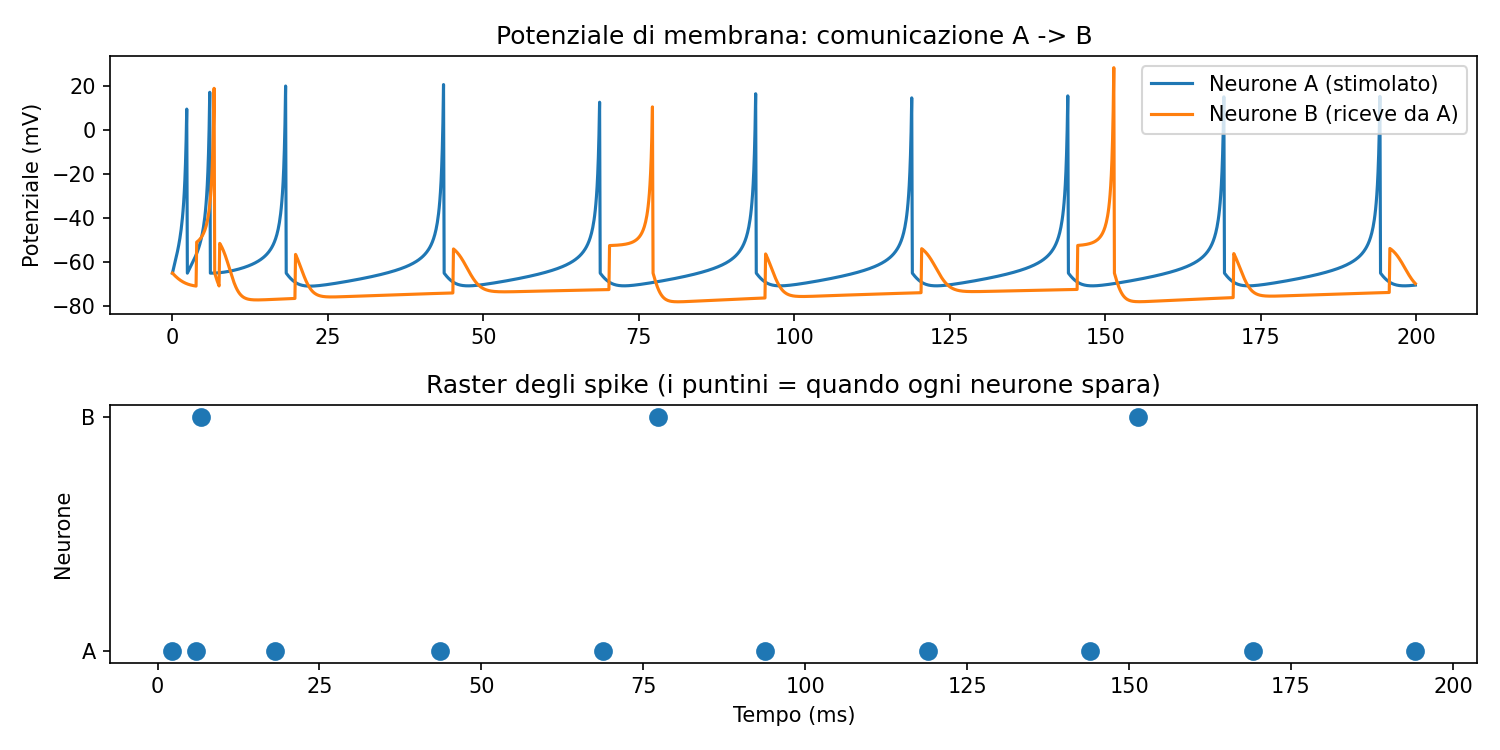
\includegraphics[width=5.8in,height=2.9in]{media/media/image1.png}

\emph{Fig. 1 --- Membrane potential and raster: A$\rightarrow$B communication.}

\textit{\textbf{Source code: due\_\allowbreak{}neuroni.py}}

\lstinputlisting[language=Python]{scripts/due_neuroni.py}
\subsection{2.2 Synaptic threshold}\label{synaptic-threshold}

The second experiment systematically explores a parameter that was set arbitrarily in the first experiment: how strong does a synapse need to be for B to respond? Varying the synaptic strength between 2 and 30 millivolts (keeping everything else identical), a sharp, nonlinear transition is observed:

{\def\LTcaptype{none} % do not increment counter
\begin{longtable}[]{@{}
  >{\raggedright\arraybackslash}p{(\linewidth - 4\tabcolsep) * \real{0.3333}}
  >{\raggedright\arraybackslash}p{(\linewidth - 4\tabcolsep) * \real{0.3333}}
  >{\raggedright\arraybackslash}p{(\linewidth - 4\tabcolsep) * \real{0.3333}}@{}}
\toprule\noalign{}
\begin{minipage}[b]{\linewidth}\raggedright
Synaptic strength (mV)
\end{minipage} & \begin{minipage}[b]{\linewidth}\raggedright
Spikes of A
\end{minipage} & \begin{minipage}[b]{\linewidth}\raggedright
Spikes of B
\end{minipage} \\
\midrule\noalign{}
\endhead
\bottomrule\noalign{}
\endlastfoot
2 & 10 & 0 \\
5 & 10 & 0 \\
10 & 10 & 0 \\
20 & 10 & 3 \\
30 & 10 & 7 \\
\end{longtable}
}

Below 10-15 millivolts neuron B never responds, no matter how many times A fires; above this threshold, B responds with an almost monotonically increasing frequency. This concretely demonstrates the concept of an activation threshold --- an intrinsically nonlinear phenomenon, not a simple proportional effect (doubling the synaptic strength from 5 to 10 mV produces no measurable change; doubling it from 10 to 20 mV produces a drastic change, from zero response to substantial response).

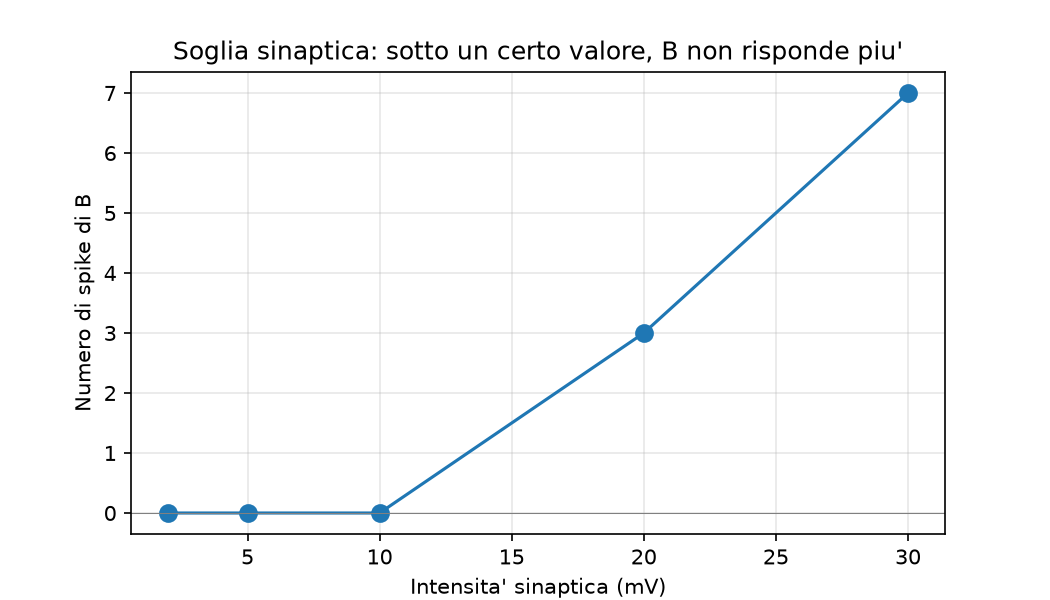
\includegraphics[width=4.5in,height=2.57143in]{media/media/image2.png}

\emph{Fig. 2 --- Synaptic threshold: a sharp transition between 10 and 20 mV.}

\textit{\textbf{Source code: esplorazione\_\allowbreak{}parametri.py}}

\lstinputlisting[language=Python]{scripts/esplorazione_parametri.py}
\subsection{2.3 Short-term synaptic plasticity (facilitation)}\label{short-term-synaptic-plasticity-facilitation}

Up to this point, synaptic strength was a fixed value, decided once and for all at the start of the simulation. The third experiment introduces the first element of dynamics: a synapse whose strength CHANGES over time depending on how it is used --- the first step, however elementary, toward the concept of synaptic "history."

The mechanism implemented is called short-term facilitation: every time A generates a spike, the weight of the synapse to B increases by a fixed increment; between one spike and the next, the weight decays exponentially toward a baseline value, with a time constant of 50 milliseconds. The result is a synaptic weight that, in the presence of closely spaced spikes, climbs progressively until it reaches a dynamic equilibrium between reinforcement and decay --- a "sawtooth" pattern clearly visible in the central panel of the figure below.

Over the course of the simulation, A produces 17 spikes and B responds with 5 --- but unlike the second experiment, A\textquotesingle s earliest spikes (when the synaptic weight is still at its baseline, sub-threshold value) do not trigger B; only after the weight has strengthened enough through repetition does B start responding.

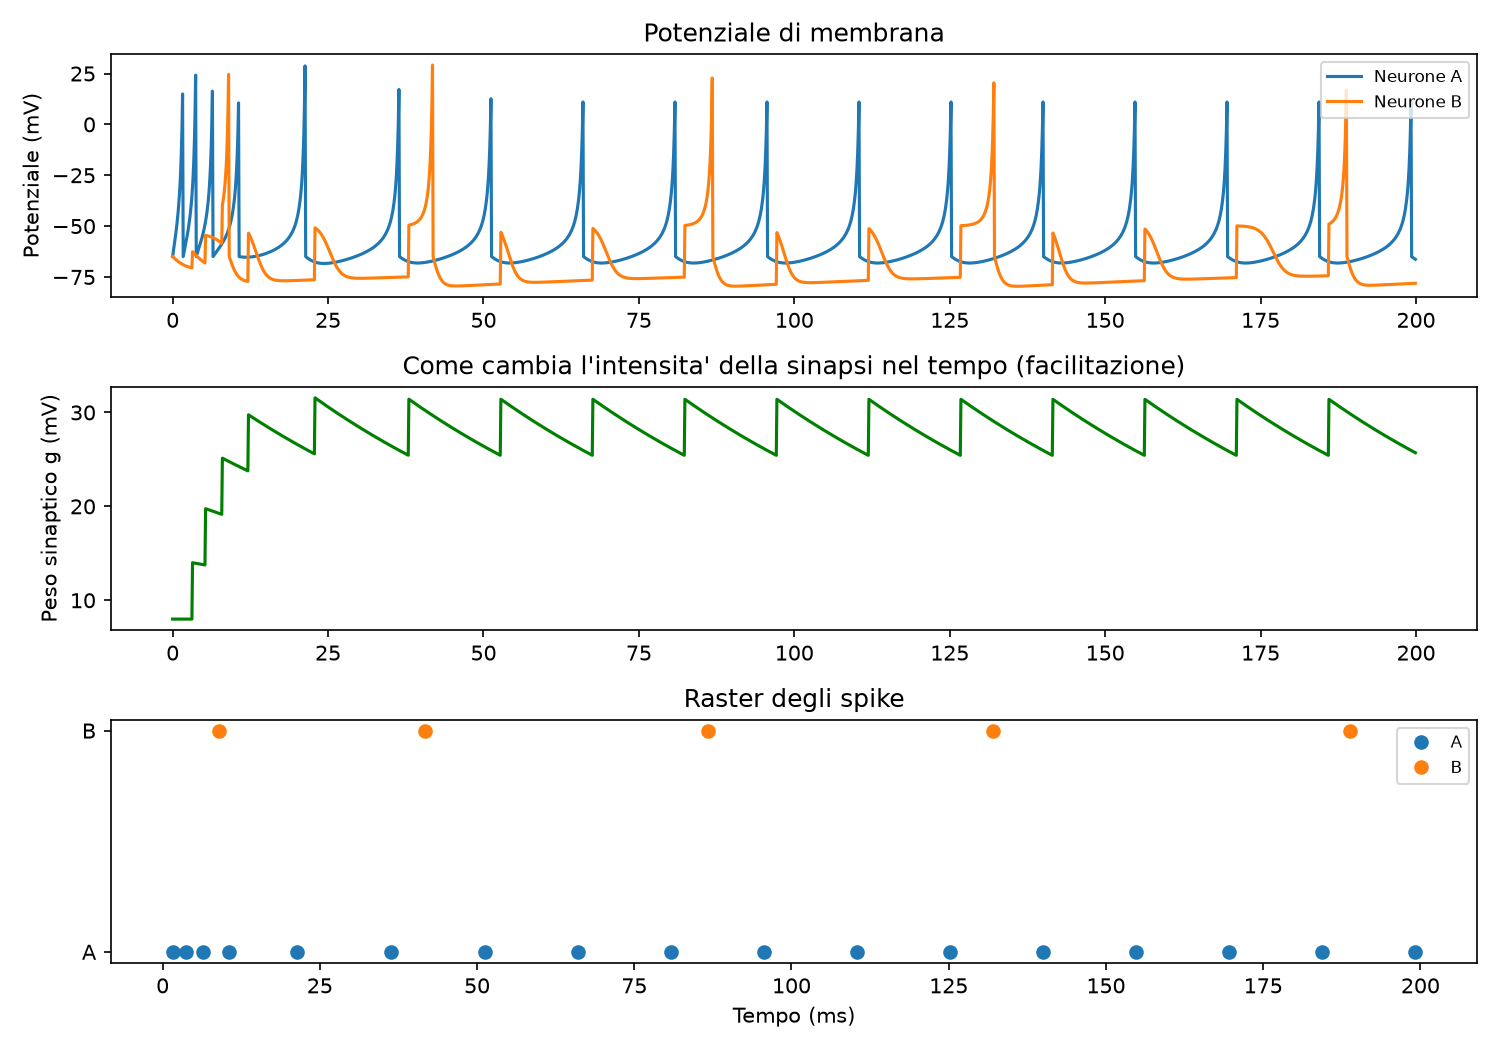
\includegraphics[width=5.8in,height=4.06in]{media/media/image3.png}

\emph{Fig. 3 --- Evolution of the synaptic weight under short-term facilitation.}

\textit{\textbf{Source code: plasticita\_\allowbreak{}sinaptica.py}}

\lstinputlisting[language=Python]{scripts/plasticita_sinaptica.py}
\subsection{2.4 Propagation along a chain of neurons}\label{propagation-along-a-chain-of-neurons}

The fourth experiment moves from two neurons to eight, connected in a linear sequence (N0$\rightarrow$N1$\rightarrow$N2$\rightarrow$...$\rightarrow$N7, each connected only to the next). Only N0 receives an external stimulus; the signal must cross the entire chain through synapses identical to those already verified.

The main result is the measurement of the propagation delay: each hop from one neuron to the next introduces about 3-4 milliseconds of delay (due to the combination of synaptic delay and the receiving neuron\textquotesingle s integration time), for a total accumulated delay of 25.9 milliseconds from the first to the last neuron in the chain. The simulation\textquotesingle s raster plot shows three distinct waves, well separated in time, each corresponding to a burst of N0 spikes propagating cleanly along the whole chain, with a diagonal pattern visible to the naked eye.

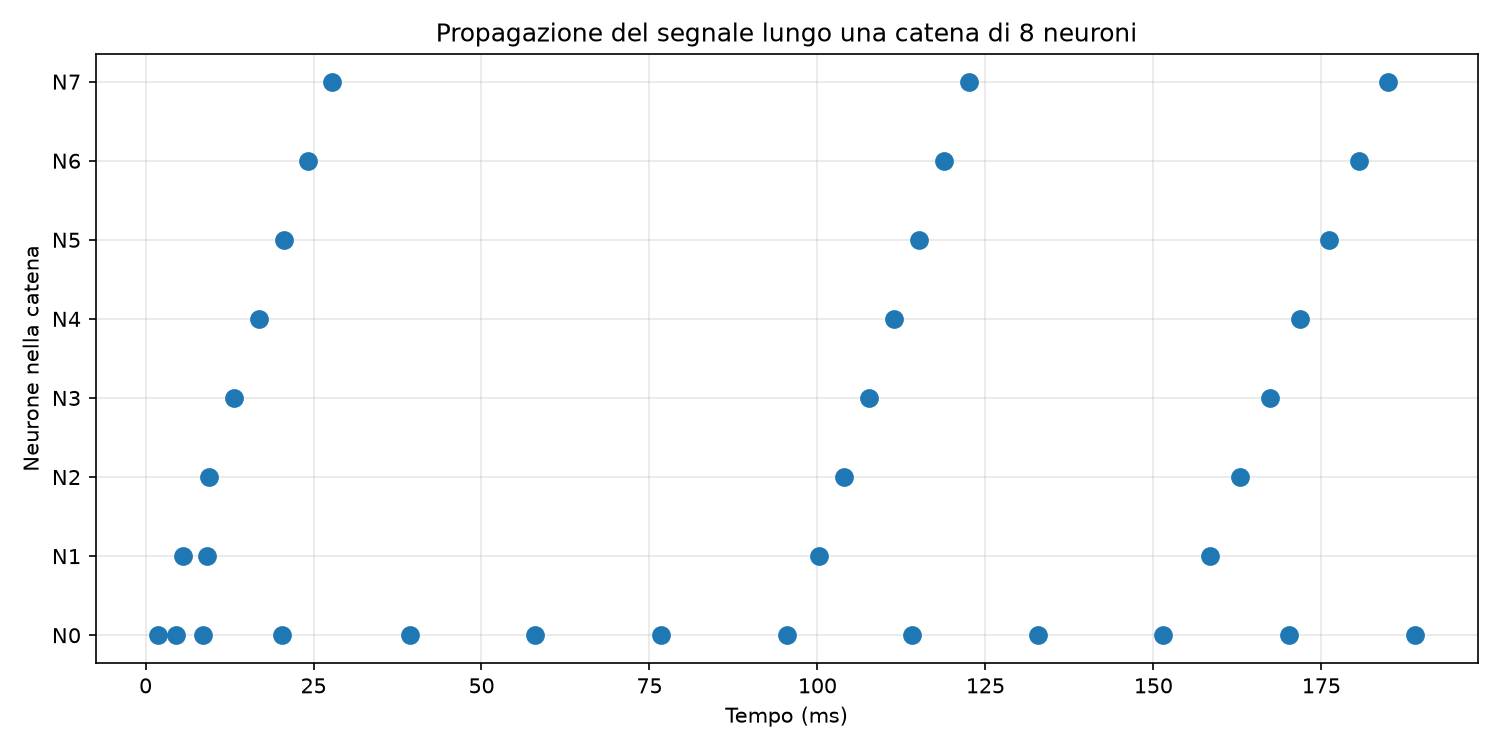
\includegraphics[width=5.8in,height=2.9in]{media/media/image4.png}

\emph{Fig. 4 --- Wave propagation along a chain of 8 neurons.}

\textit{\textbf{Source code: rete\_\allowbreak{}catena.py}}

\lstinputlisting[language=Python]{scripts/rete_catena.py}
\subsection{2.5 Temporal summation (convergence)}\label{temporal-summation-convergence}

The fifth experiment reverses the topology: instead of a linear chain, three independent neurons (N0, N1, N2) converge onto a fourth, target neuron (N3). Each of the three source neurons fires exactly once, with the exact same synaptic strength (10 mV) onto N3 in both tested scenarios.

In the "synchronous" scenario, the three spikes arrive at the same instant (t=10ms): N3 receives all the input together, its potential jumps and crosses threshold --- N3 fires. In the "staggered" scenario, the same three spikes arrive 5 milliseconds apart from one another (t=10, 15, 20ms): N3\textquotesingle s potential rises in small steps but decays between one input and the next, never reaching threshold --- N3 never fires, despite having received exactly the same total amount of stimulation.

This demonstrates the principle of temporal summation, or "coincidence detection": a neuron counts not only HOW MANY inputs it receives, but HOW CLOSE TOGETHER they are in time. It is one of the most fundamental computational mechanisms by which a single neuron can act as a detector of correlations among incoming signals.

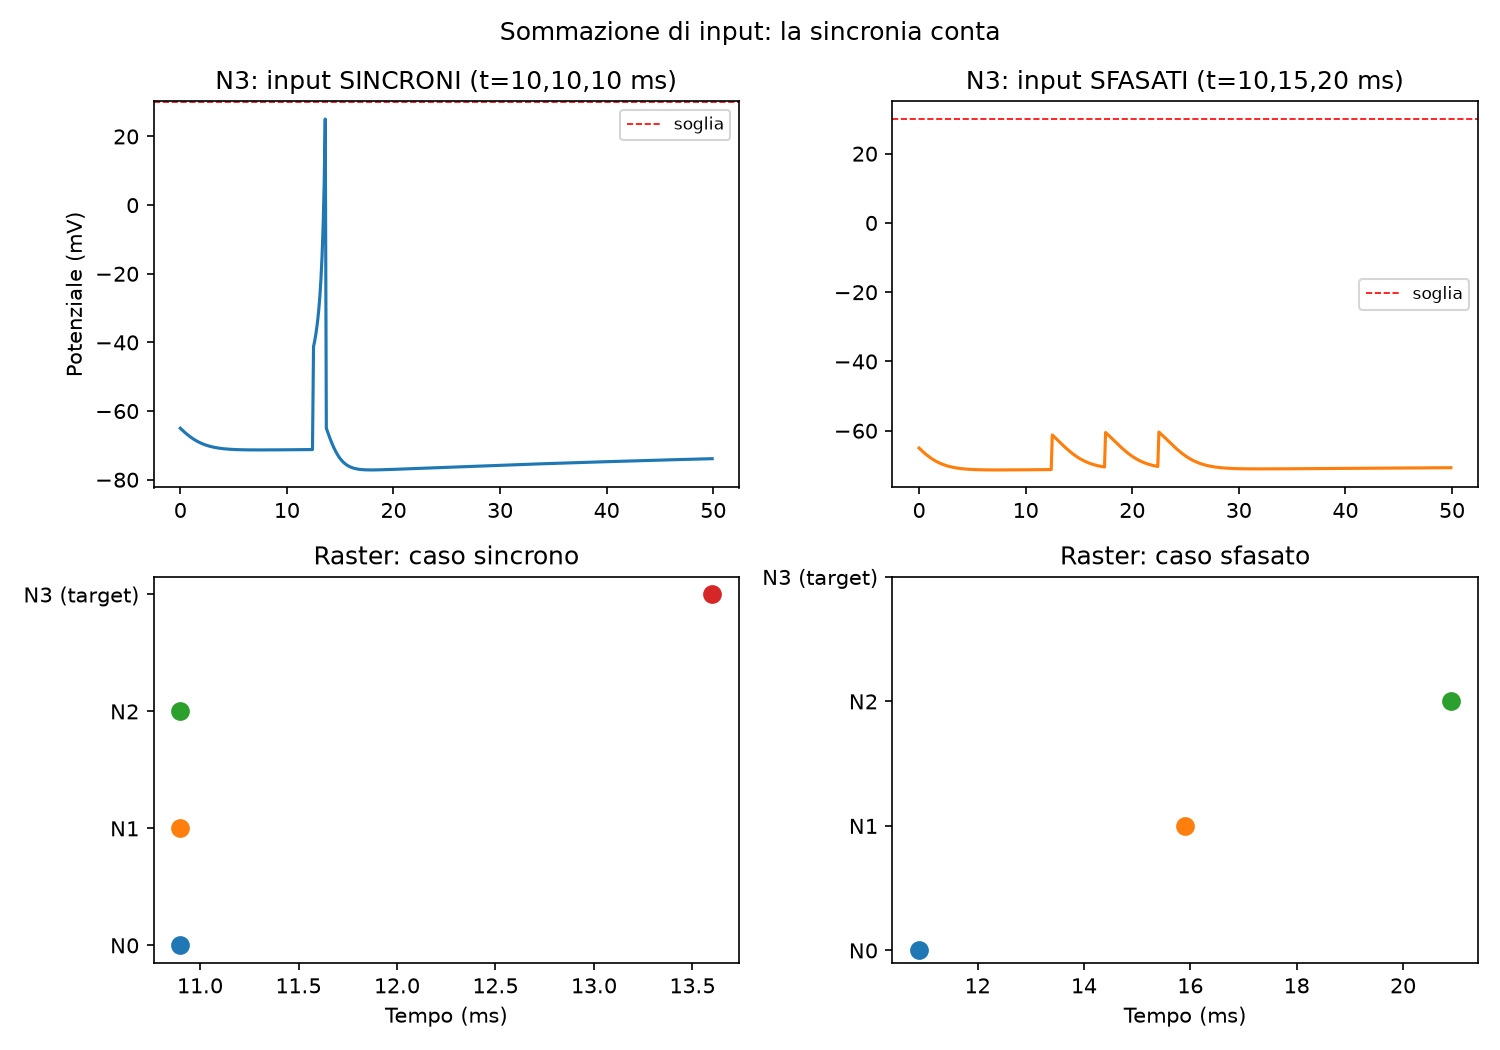
\includegraphics[width=5.8in,height=4.06in]{media/media/image5.png}

\emph{Fig. 5 --- Temporal summation: synchronous vs. staggered inputs.}

\textit{\textbf{Source code: rete\_\allowbreak{}convergente.py}}

\lstinputlisting[language=Python]{scripts/rete_convergente.py}
\subsection{2.6 STDP --- Spike-Timing-Dependent Plasticity}\label{stdp-spike-timing-dependent-plasticity}

The sixth experiment replaces the simple short-term facilitation of experiment 2.3 with a much more realistic learning rule, and one far more widely used in the computational neuroscience literature: Spike-Timing-Dependent Plasticity (STDP), often summarized by the mnemonic "neurons that fire together, wire together" (the temporal version of Hebb\textquotesingle s rule, 1949).

The principle: if the presynaptic neuron (A) systematically fires SHORTLY BEFORE the postsynaptic neuron (B), the synapse A$\rightarrow$B is STRENGTHENED (potentiation, LTP --- Long-Term Potentiation), because A appears to "predict" B, a potentially causal relationship. If instead A fires SHORTLY AFTER B, the synapse is WEAKENED (depression, LTD). The Brian2 implementation uses two exponential trace variables (apre, apost) that accumulate at every spike and decay with a time constant of 20 milliseconds --- the standard mechanism for implementing STDP efficiently without having to explicitly compare every pair of past spikes.

Verified over 5 repetitions of a fixed pattern, "A fires 5 milliseconds before B": the synaptic weight rises monotonically, in steps, from an initial value of 5.00 mV to 8.36 mV after the 5 repetitions --- a net strengthening of 3.36 mV entirely attributable to the STDP rule.

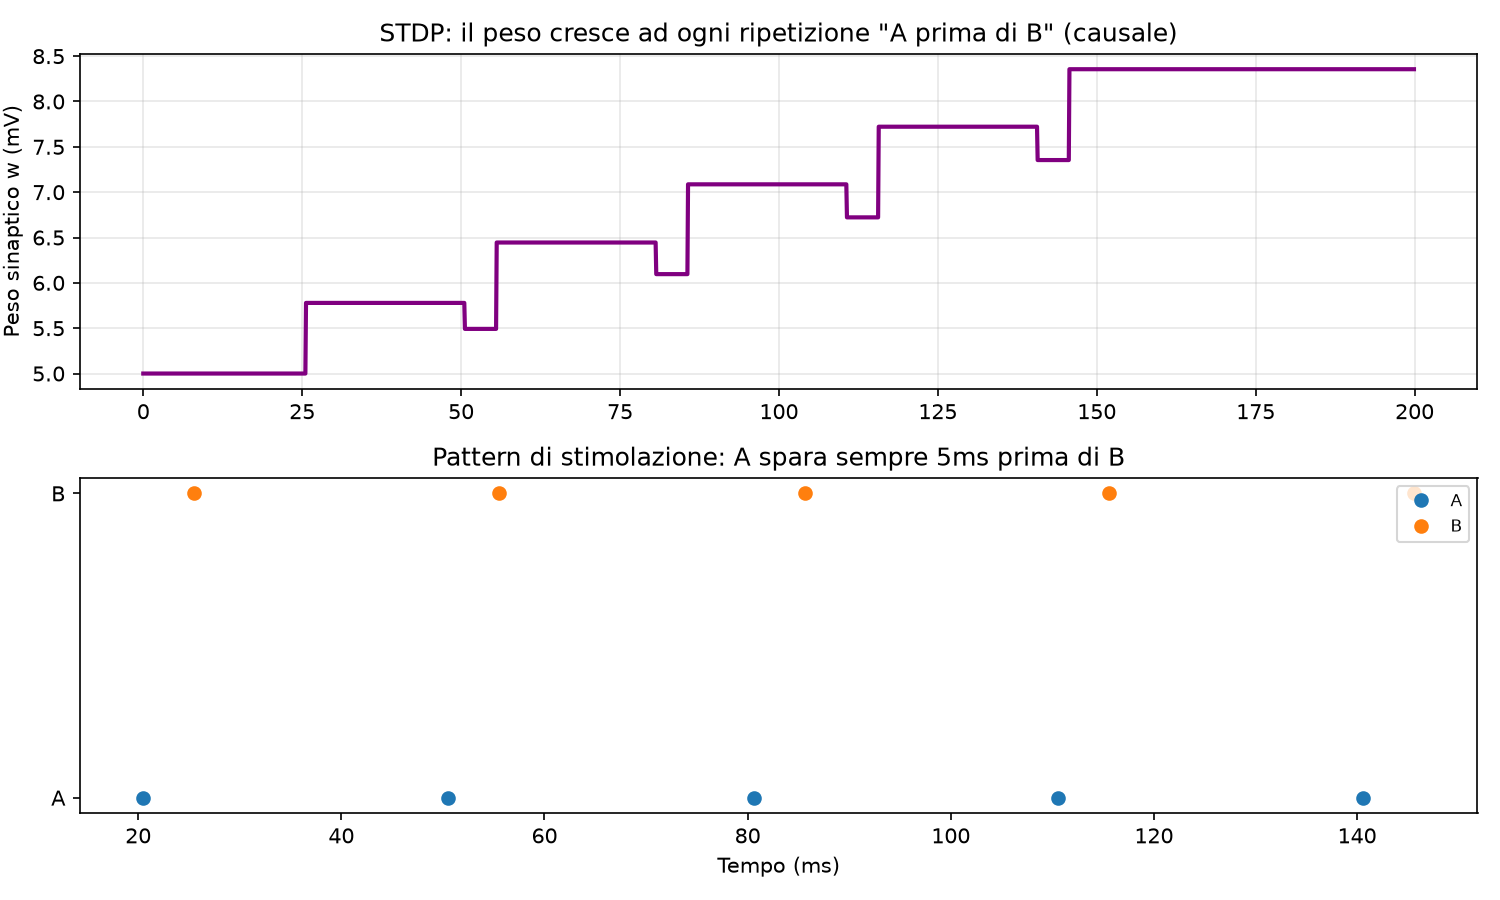
\includegraphics[width=5.5in,height=3.3in]{media/media/image6.png}

\emph{Fig. 6 --- Strengthening of the synaptic weight via STDP over causal repetitions.}

\textit{\textbf{Source code: stdp.py}}

\lstinputlisting[language=Python]{scripts/stdp.py}
\subsection{2.7 Pattern classification via STDP}\label{pattern-classification-via-stdp}

The seventh experiment is the project\textquotesingle s first major conceptual leap: no longer just observing how a SINGLE synaptic weight changes, but checking whether an entire small circuit can LEARN to distinguish two different input patterns, without anyone explicitly writing the rule for telling them apart.

Structure: 6 input neurons, split into two groups of 3 (Group A and Group B, representing two distinct "patterns"). An output neuron O receives from all 6 via plastic STDP synapses, with initial weights all equal and low (6 mV). During training (10 repetitions), every time Pattern A is presented, a small external "teacher" forces O to fire right afterward --- like a teacher guiding the correct response. When Pattern B is presented, no external help is given.

In the TEST phase, with no external help at all: Pattern A presented alone makes O fire; Pattern B presented alone does NOT make it fire. The final weights confirm the mechanism: Group A\textquotesingle s synapses have risen to saturate at the maximum allowed value (15.00 mV), while Group B\textquotesingle s have stayed close to their initial value, if anything slightly weakened (5.67 mV). The discriminative behavior --- responding selectively to one pattern and not the other --- EMERGED from the STDP rule applied repeatedly; it was never written explicitly anywhere in the code as an "if pattern == A" condition.

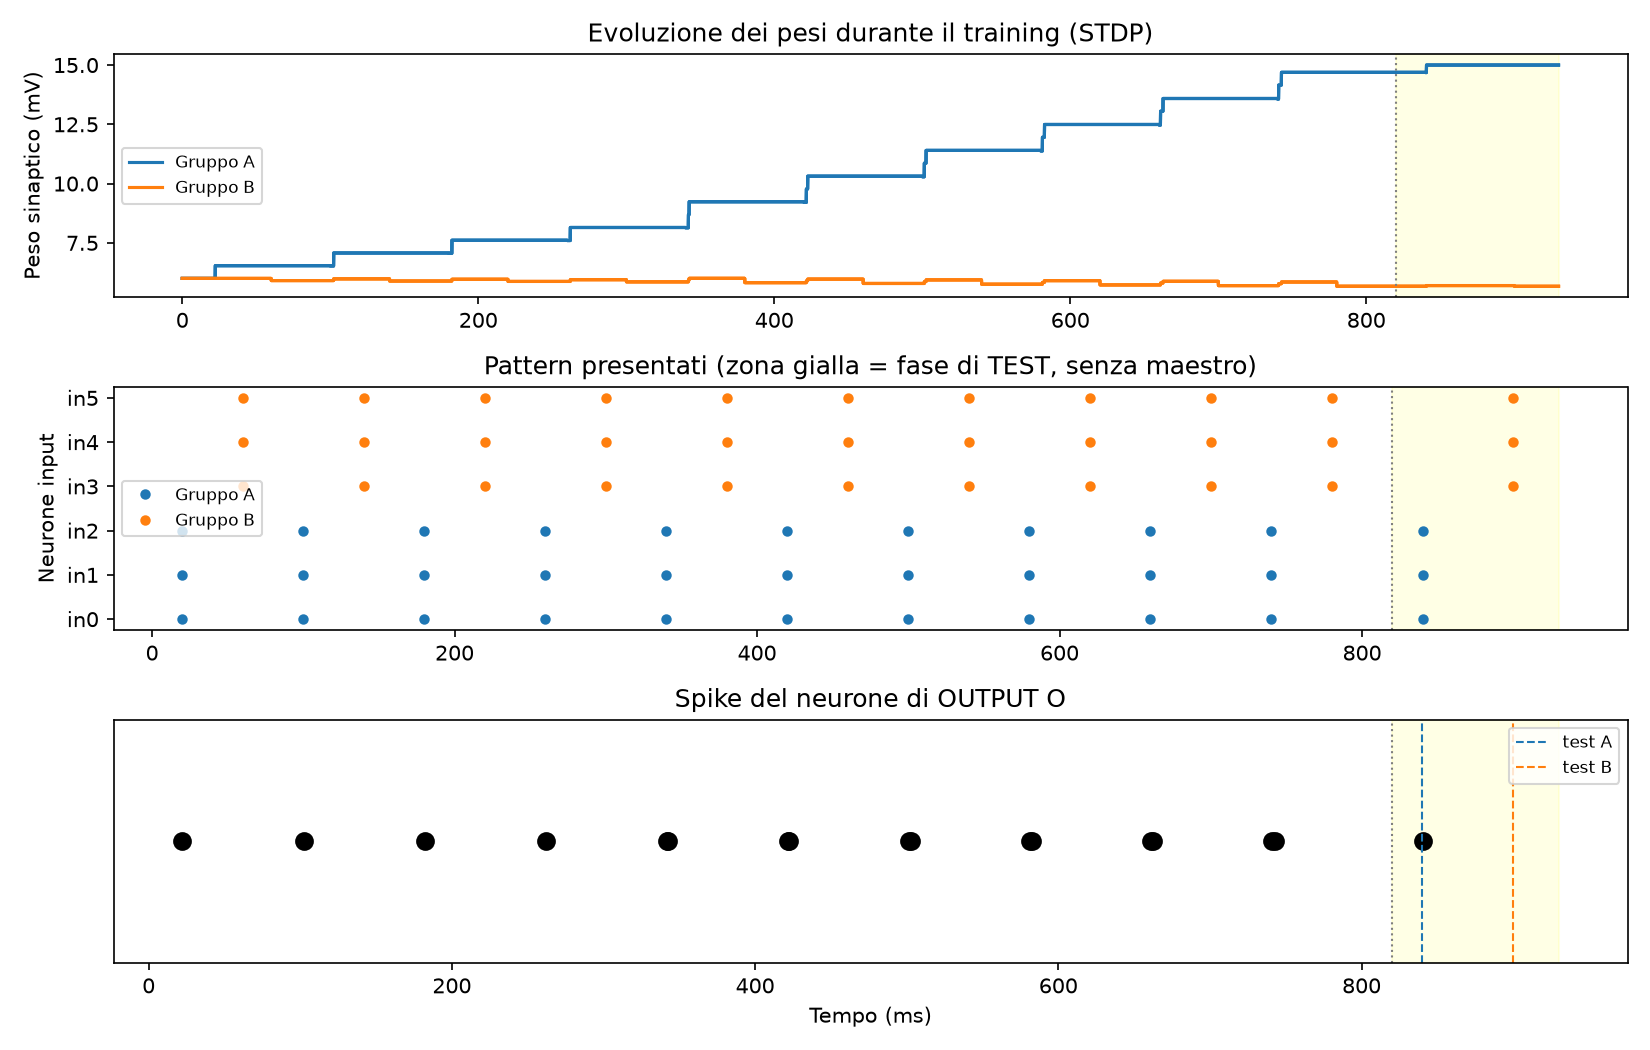
\includegraphics[width=5.8in,height=3.69091in]{media/media/image7.png}

\emph{Fig. 7 --- Selective learning: response to Pattern A only, after training.}

\textit{\textbf{Source code: classificazione\_\allowbreak{}stdp.py}}

\lstinputlisting[language=Python]{scripts/classificazione_stdp.py}
\subsection{2.8 Balanced excitation-inhibition network (300 neurons)}\label{balanced-excitation-inhibition-network-300-neurons}

The eighth experiment is the project\textquotesingle s first real jump in scale: from a handful of neurons to 300, organized according to the standard architecture from the computational neuroscience literature for networks of this size --- the "balanced" model inspired by the work of Nicolas Brunel (2000).

The network is made of 240 excitatory neurons (80\%, which push target neurons toward spiking) and 60 inhibitory neurons (20\%, which suppress activity), with sparse, random 10\% connectivity (each pair of neurons has a 10\% probability of being connected, independently of every other pair). A preliminary attempt with excitatory synapses only (not shown in detail in this document, but verified during development) makes the network either explode into a synchronized discharge of the whole population, or shut down entirely --- neither behavior is interesting or realistic.

Introducing inhibition in the correct proportion instead produces a state of activity known as "asynchronous irregular": neurons fire at an average frequency of about 15.6 Hz, in a statistically structured way but without all synchronizing together --- qualitatively similar to the activity observed in real cerebral cortex during wakefulness.

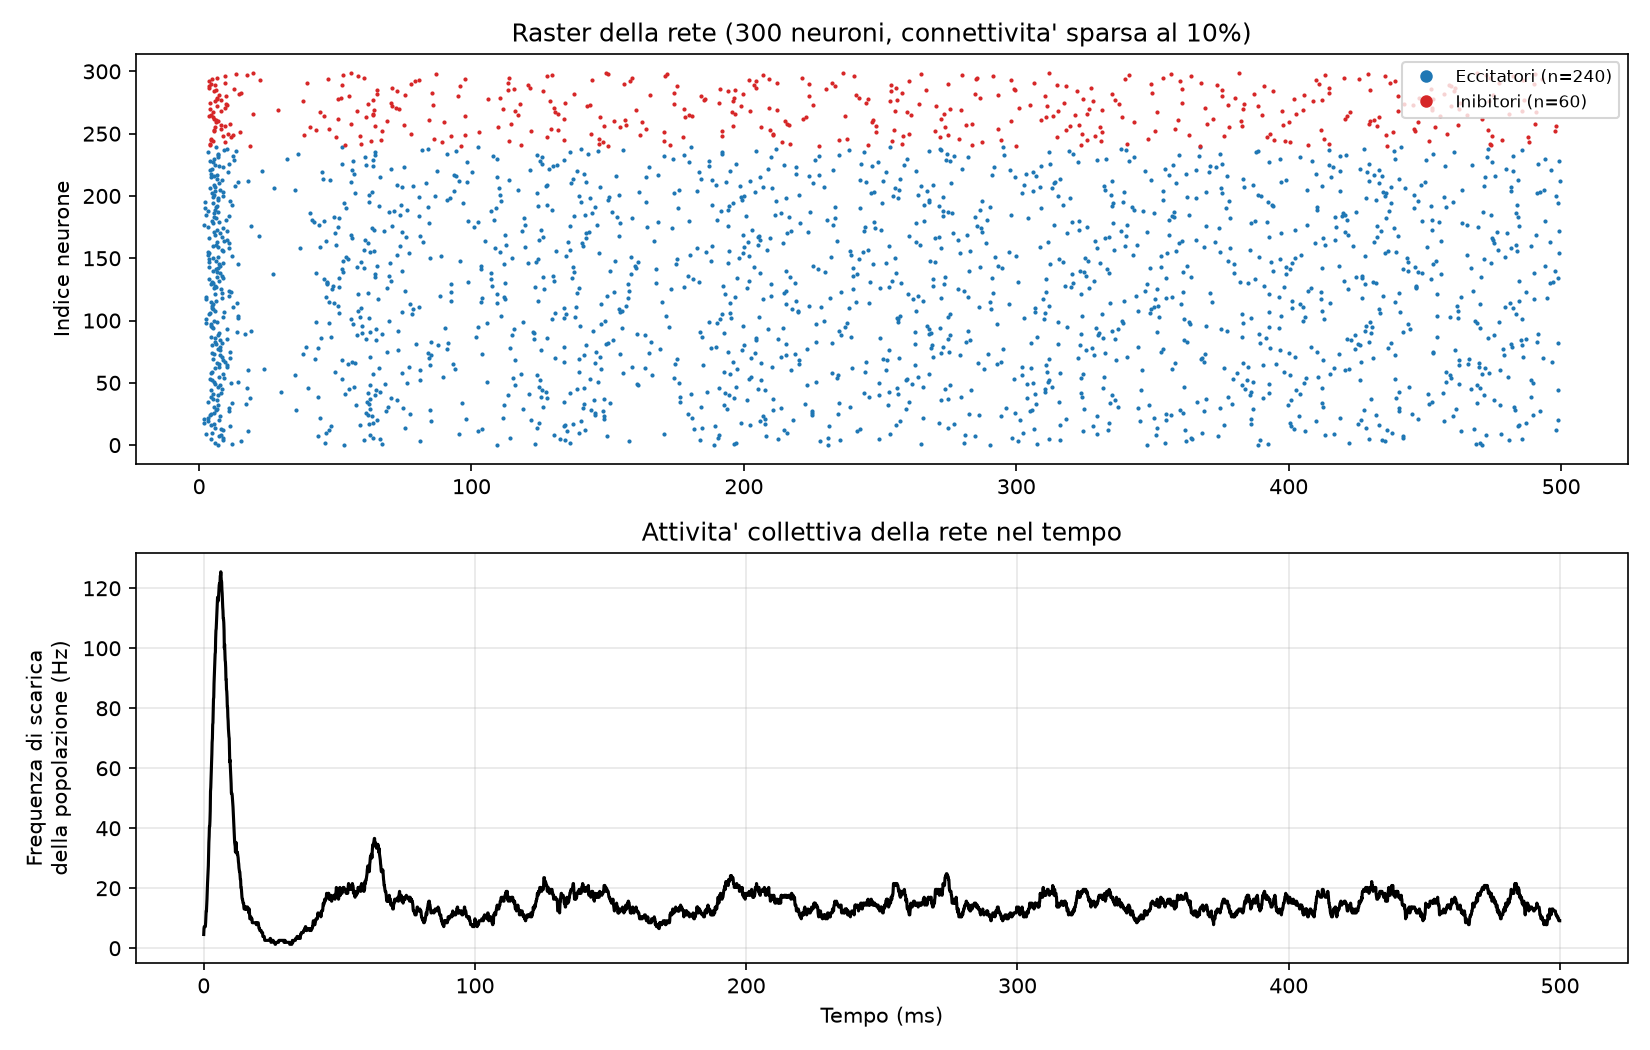
\includegraphics[width=5.8in,height=3.69091in]{media/media/image8.png}

\emph{Fig. 8 --- Raster and collective frequency of the 300-neuron network.}

\textit{\textbf{Source code: rete\_\allowbreak{}300\_\allowbreak{}neuroni.py}}

\lstinputlisting[language=Python]{scripts/rete_300_neuroni.py}
\subsection{2.9 Response to a stimulus and homeostatic recovery}\label{response-to-a-stimulus-and-homeostatic-recovery}

The ninth experiment checks how the 300-neuron network, already stable in its spontaneous-activity state, responds to an external perturbation. A strong current pulse is applied to just 20 out of 300 neurons (6.7\% of the network) for 20 milliseconds, then removed entirely.

The network\textquotesingle s collective frequency jumps sharply from about 14.9 Hz (baseline) to a peak of about 68.6 Hz during and right after the stimulus, then spontaneously returns to the starting level (15.6 Hz) with no external intervention. An interesting detail, clearly visible in the plot: after the peak, the frequency does not glide gently back to baseline but briefly dips BELOW the starting level (an inhibitory "undershoot") before restabilizing --- a behavior typical of negative-feedback systems, where the inhibitory neurons activated by the excitatory wave stay active a moment longer than strictly necessary.

This behavior --- a proportionate response to a stimulus, followed by a spontaneous return to equilibrium --- is the project\textquotesingle s first appearance of something resembling HOMEOSTASIS, a fundamental property of any functioning nervous system: the ability to respond without staying "damaged" or entering a pathological regime.

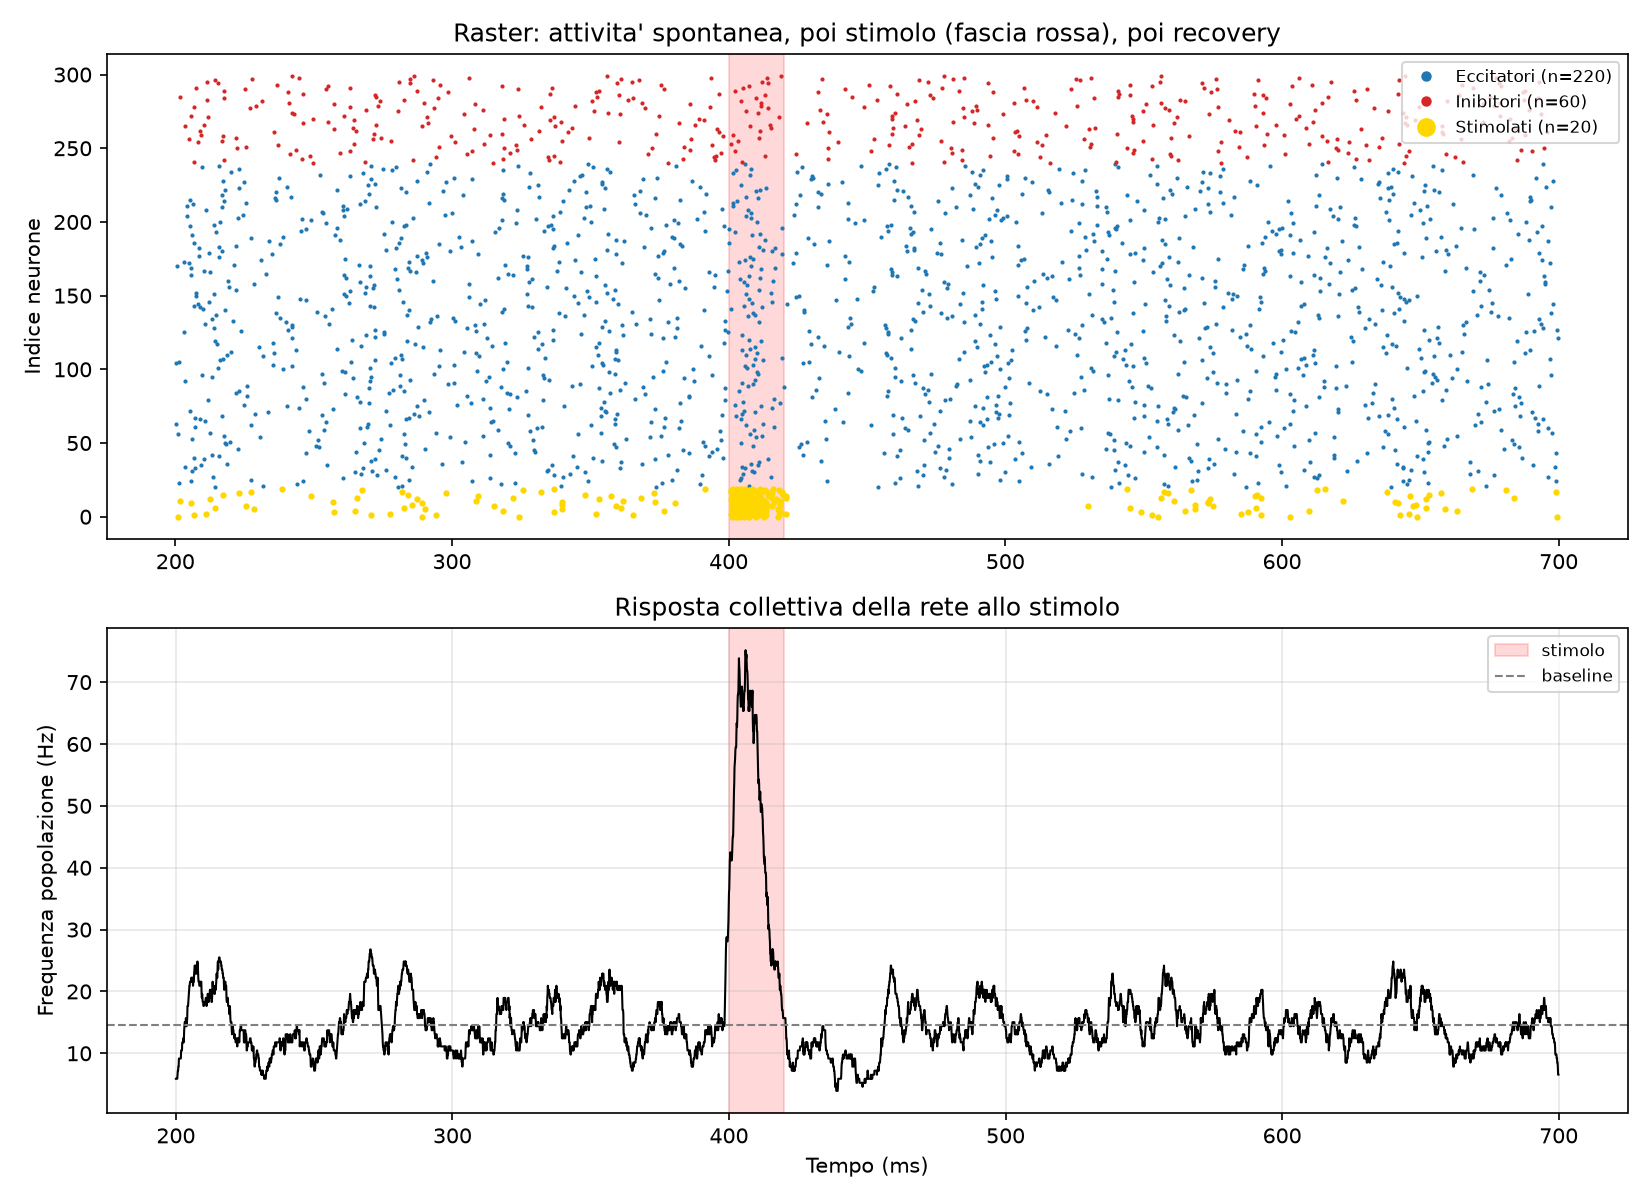
\includegraphics[width=5.8in,height=4.21818in]{media/media/image9.png}

\emph{Fig. 9 --- Homeostatic response and recovery after a targeted stimulus.}

\textit{\textbf{Source code: rete\_\allowbreak{}300\_\allowbreak{}stimolo.py}}

\lstinputlisting[language=Python]{scripts/rete_300_stimolo.py}
\subsection{2.10 Modular architecture: two connected regions}\label{modular-architecture-two-connected-regions}

The tenth experiment introduces, for the first time in the project, the concept of distinct REGIONS, rather than a single undifferentiated mass of neurons. The 300-neuron network is split into two modules of 150 each (identical internal E/I structure, dense 10\% connectivity as before), but connected to each other only weakly: a 2\% connection probability, and ONLY excitatory synapses --- a choice that mirrors how long-range cortico-cortical connections actually work in the real brain, typically excitatory and relatively sparse compared to the connection density within a single area.

Stimulating ONLY Module 1 (20 neurons, as in experiment 2.9), a single trial shows an apparent increase in activity even in Module 2, which received no direct stimulus: +88 Hz in Module 1 (directly stimulated) and +13 Hz in Module 2 (attenuated but apparently present). At first glance, this would seem to demonstrate that the signal propagates between the two regions through the few connections linking them.

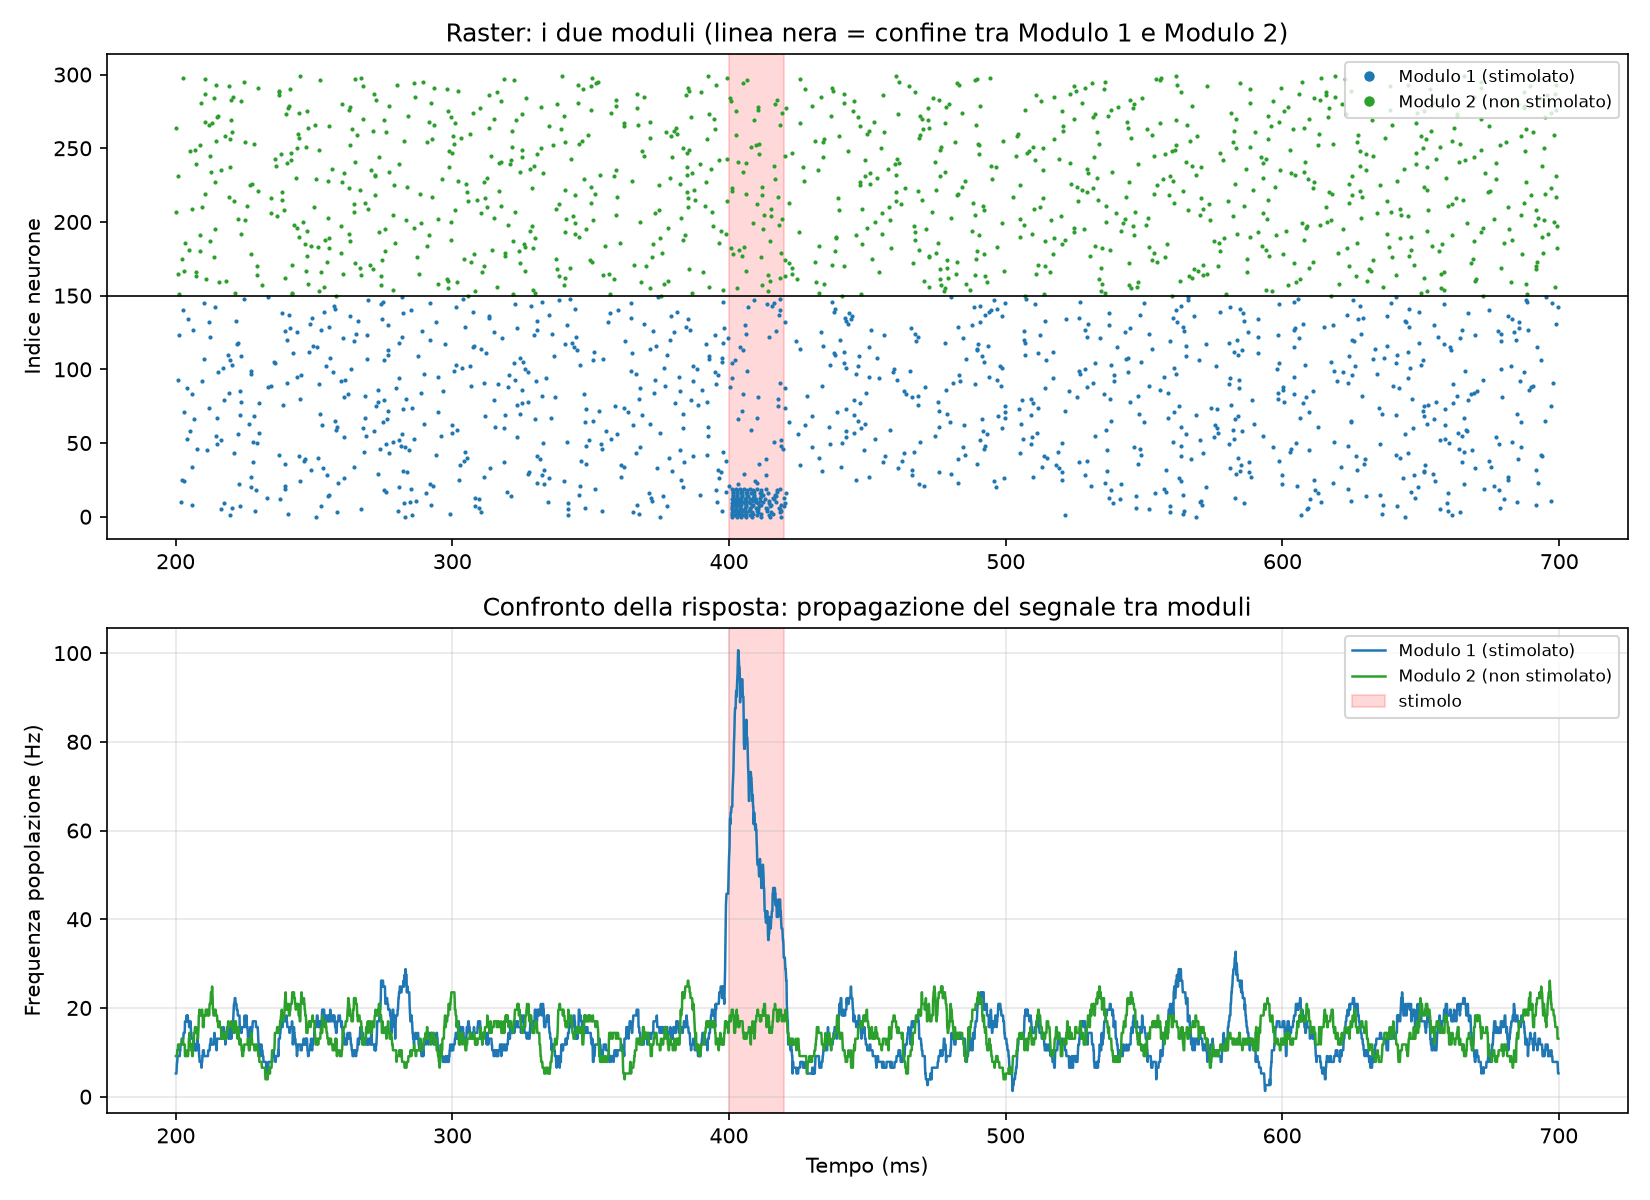
\includegraphics[width=5.8in,height=4.21818in]{media/media/image10.png}

\emph{Fig. 10 --- Apparent propagation between modules (single trial).}

\textit{\textbf{Source code: due\_\allowbreak{}moduli.py}}

\lstinputlisting[language=Python]{scripts/due_moduli.py}
\subsection{2.11 Statistical verification: is the observed effect real or noise?}\label{statistical-verification-is-the-observed-effect-real-or-noise}

\textbf{The eleventh experiment is, from a methodological standpoint, probably the most important in the entire project --- not for the positive result it produces, but for what it TEACHES about the scientific rigor needed before drawing conclusions.}

Looking closely at the plot from experiment 2.10, the small increase in Module 2 activity (+13 Hz) turned out to be comparable in size to the network\textquotesingle s normal spontaneous fluctuations, visible elsewhere in the same plot even with no stimulus underway. A single trial does not allow one to distinguish a real propagation effect from a statistical coincidence.

The solution adopted is the standard technique used in experimental neuroscience for exactly this problem: the PSTH (Peristimulus Time Histogram). The identical experiment is repeated 25 times, each trial is aligned to the exact moment of the stimulus, and the AVERAGE is computed across all trials --- if a real effect exists, it clearly emerges above the noise in the average (which tends to cancel out when averaging over many independent repetitions); if no real effect exists, the average stays flat.

Result of the check: the average effect measured in Module 2, averaged over 25 repetitions, came out to just +0.89 Hz --- clearly within the background noise (the standard deviation of a single trial, measured over the same time window, is about 4 Hz, nearly 5 times larger than the observed average effect).

\textbf{Honest conclusion: with these connectivity parameters (2\% probability, excitatory synapses only), it is NOT possible to confidently claim that the signal propagates meaningfully between the two modules. What looked like a clear effect in the single trial was, in all likelihood, largely random statistical noise.}

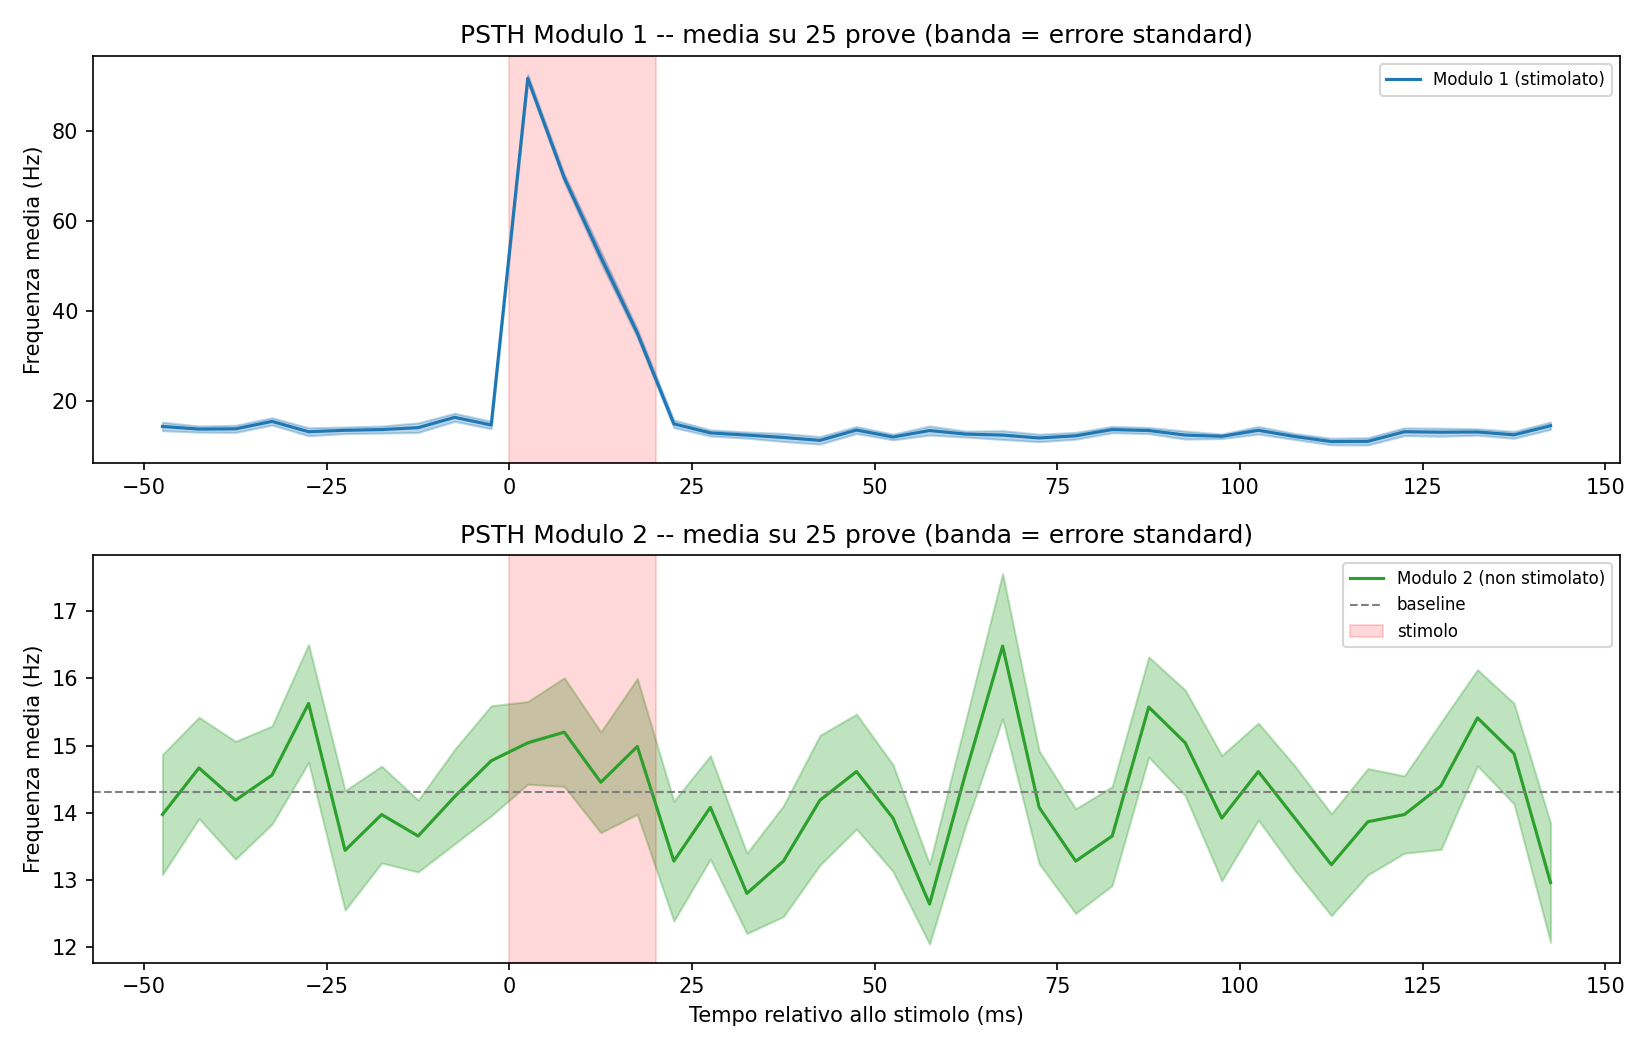
\includegraphics[width=5.8in,height=3.69091in]{media/media/image11.png}

\emph{Fig. 11 --- PSTH over 25 trials: the average effect falls within the noise.}

This negative result, obtained with the correct statistical tool, is probably the most solid contribution of the entire project from the standpoint of scientific method: it shows the concrete difference between a result that SEEMS interesting at first glance and a result VERIFIED with the appropriate statistical tools --- a distinction that recurs, in different forms, later in the document as well (Section 4.2, Section 5.3).

\textit{\textbf{Source code: psth\_\allowbreak{}moduli.py}}

\lstinputlisting[language=Python]{scripts/psth_moduli.py}
\section{3. Scaling toward the size of a mouse brain}\label{scaling-toward-the-size-of-a-mouse-brain}

\subsection{3.1 The reference number and the memory constraint}\label{the-reference-number-and-the-memory-constraint}

A mouse brain has about 70 million neurons, counting the whole brain (cerebellum included). Simulating it in full, at a level of biophysical detail comparable to what this project uses, is beyond the reach of a single laptop --- but it was possible to measure, step by step and with real data (not estimated on paper), how close one could realistically get with the available hardware: a MacBook Air M5 with 24 GB of total RAM.

The dominant constraint, as the data in this section clearly show, turned out to be available RAM memory, not raw compute speed --- an interesting empirical finding in its own right, since one might initially have expected the opposite.

\subsection{3.2 The key technical change: fixed-degree connectivity}\label{the-key-technical-change-fixed-degree-connectivity}

To scale beyond a few thousand neurons, it was necessary to abandon Brian2\textquotesingle s standard syntax for probabilistic connectivity. The reason is purely computational: the connect(condition=..., p=...) syntax conceptually evaluates the connection probability for EVERY possible pair of neurons in the network --- a cost that grows as the square of the neuron count (N\textsuperscript{2}). For a network of 40 million neurons, N\textsuperscript{2} would be on the order of 1.6 $\times$ 10\textsuperscript{1}\textsuperscript{5} --- a completely impractical number to process, even just to generate the list of synapses, no matter how long one were willing to wait.

The solution adopted is FIXED-DEGREE connectivity: instead of a connection probability evaluated over all possible pairs, each neuron connects to exactly K other neurons (K=15 in this project), chosen at random from the whole network. The total number of synapses thus grows LINEARLY with N (about K$\times$N total synapses per connection type), not quadratically --- and it is precisely this difference, between linear and quadratic growth, that makes it possible to scale to millions of neurons instead of getting stuck at a few thousand.

\emph{Fixed-probability connectivity: N\_\allowbreak{}synapses $\approx$ p $\times$ N\textsuperscript{2} (impractical beyond N\textasciitilde10\textsuperscript{4})}

\emph{Fixed-degree connectivity: N\_\allowbreak{}synapses $\approx$ K $\times$ N (practical up to N\textasciitilde10\textsuperscript{7}-10\textsuperscript{8})}

\subsection{3.3 Scaling data, measured on the MacBook Air M5}\label{scaling-data-measured-on-the-macbook-air-m5}

The table below reports ALL the data points collected during the scaling phase, measured directly on the author\textquotesingle s MacBook Air M5 across four successive test sessions ("phase 1" through "phase 4"), each pushing the network size a bit higher than the last, recalibrating the predictive memory estimate each time on the real data already collected (rather than on a purely theoretical model), to avoid risking a system crash from running out of RAM.

{\def\LTcaptype{none} % do not increment counter
\begin{longtable}[]{@{}
  >{\raggedright\arraybackslash}p{(\linewidth - 8\tabcolsep) * \real{0.2000}}
  >{\raggedright\arraybackslash}p{(\linewidth - 8\tabcolsep) * \real{0.2000}}
  >{\raggedright\arraybackslash}p{(\linewidth - 8\tabcolsep) * \real{0.2000}}
  >{\raggedright\arraybackslash}p{(\linewidth - 8\tabcolsep) * \real{0.2000}}
  >{\raggedright\arraybackslash}p{(\linewidth - 8\tabcolsep) * \real{0.2000}}@{}}
\toprule\noalign{}
\begin{minipage}[b]{\linewidth}\raggedright
N neurons
\end{minipage} & \begin{minipage}[b]{\linewidth}\raggedright
N synapses
\end{minipage} & \begin{minipage}[b]{\linewidth}\raggedright
Time (s)
\end{minipage} & \begin{minipage}[b]{\linewidth}\raggedright
RAM (MB)
\end{minipage} & \begin{minipage}[b]{\linewidth}\raggedright
\% of mouse brain
\end{minipage} \\
\midrule\noalign{}
\endhead
\bottomrule\noalign{}
\endlastfoot
1,000 & 31,000 & 1.12 & 301 & 0.001\% \\
10,000 & 310,000 & 9.04 & 330 & 0.014\% \\
100,000 & 3,100,000 & 1.37 & 444 & 0.143\% \\
500,000 & 15,500,000 & 6.44 & 873 & 0.714\% \\
1,000,000 & 31,000,000 & 12.91 & 1,720 & 1.429\% \\
3,000,000 & 93,000,000 & 38.85 & 4,152 & 4.286\% \\
5,000,000 & 155,000,000 & 65.66 & 6,254 & 7.143\% \\
10,000,000 & 310,000,000 & 133.28 & 9,838 & 14.286\% \\
20,000,000 & 620,000,000 & 269.71 & 11,147 & 28.571\% \\
25,000,000 & 775,000,000 & 336.75 & 11,495 & 35.714\% \\
30,000,000 & 930,000,000 & 405.57 & 12,434 & 42.857\% \\
35,000,000 & 1,085,000,000 & 497.05 & 15,104 & 50.000\% \\
40,000,000 & 1,240,000,000 & 573.08 & 15,744 & 57.143\% \\
\end{longtable}
}

At 50 million neurons (predicted estimate \textasciitilde21-25 GB of RAM), the attempt was aborted after more than an hour without completing even 200 milliseconds of simulated time. Analysis via macOS Activity Monitor revealed the cause: not an imminent crash, but very heavy memory compression by the operating system (visible as "yellow", not critical "red", memory pressure), which kept the CPU busy (77-95\% utilization) without the actual computation advancing proportionally --- the classic sign of a system spending most of its time compressing and decompressing data in memory instead of performing the requested computation. The attempt was stopped manually as a precaution.

\textbf{The practical limit verified and completed with full success therefore remains 40 million neurons --- 57.1\% of mouse-brain scale.}

\subsection{3.4 Effect of thermal throttling}\label{effect-of-thermal-throttling}

A phenomenon observed only in the final, most extended experiment (Section 3.6, with several phases simulated in sequence and a much longer total duration than the individual scaling benchmarks): the MacBook Air, being a model with no active cooling fan, progressively slows its own performance under sustained computational load to protect itself from overheating --- a standard protective behavior in modern processors, known as thermal throttling.

The single scaling benchmark of 200 milliseconds of simulated time, at 40 million neurons, had taken 573 seconds (just over 9 minutes). The final experiment in Section 3.6, with 700 milliseconds of total simulated time split across four sequential phases (burn-in, baseline, stimulus, recovery), instead took several HOURS of real time --- a 3-4x slowdown relative to what a simple linear projection from the scaling data would have predicted. The most likely cause, verified indirectly by monitoring CPU usage during execution (which showed consistently high utilization, 85-95\%, ruling out a hang or an error), is cumulative thermal throttling over a long run: after tens of minutes at full load, the chip progressively lowers its own clock frequency to contain temperature, even though the workload itself does not change.

\subsection{3.5 Progressive scaling script: methodology}\label{progressive-scaling-script-methodology}

The scripts used for progressive scaling implement a two-level safety strategy, to avoid risking a system freeze during automated tests over progressively larger sizes: a PREDICTIVE estimate of the memory required (based on a linear regression over the data points already collected in earlier phases, with a percentage safety margin), computed BEFORE attempting a new size; and a maximum time limit per single attempt, past which the script stops automatically. The combination of the two mechanisms allowed automatic, progressively more ambitious exploration, with no need for constant supervision, up to the system\textquotesingle s real limit.

\textit{\textbf{Source code: scaling\_\allowbreak{}fase4.py (the last of the 4 automatic scaling phases)}}

\lstinputlisting[language=Python]{scripts/scaling_fase4.py}
\subsection{3.6 Final experiment at 40 million neurons}\label{final-experiment-at-40-million-neurons}

Once the practical achievable limit had been established, a complete experiment was built at the maximum verified scale, repeating the same experimental structure already validated at 300 neurons in Section 2.9 (baseline, targeted stimulus, recovery), but this time with specific memory precautions given the enormously larger scale: instead of recording spike times for all 40 million neurons (which would have required a prohibitive amount of memory), only the AGGREGATE firing rate of the ENTIRE population over time was recorded (via an efficient rate monitor that does not save every single spike, only the aggregate trend), together with a detailed raster of a small subset of 2,000 neurons, enough for a representative visual snapshot without overloading available memory.

{\def\LTcaptype{none} % do not increment counter
\begin{longtable}[]{@{}
  >{\raggedright\arraybackslash}p{(\linewidth - 2\tabcolsep) * \real{0.5000}}
  >{\raggedright\arraybackslash}p{(\linewidth - 2\tabcolsep) * \real{0.5000}}@{}}
\toprule\noalign{}
\begin{minipage}[b]{\linewidth}\raggedright
Phase
\end{minipage} & \begin{minipage}[b]{\linewidth}\raggedright
Mean population frequency
\end{minipage} \\
\midrule\noalign{}
\endhead
\bottomrule\noalign{}
\endlastfoot
Baseline (before stimulus) & 14.49 Hz \\
Peak during/after stimulus & 17.74 Hz \\
After recovery & 14.31 Hz \\
\end{longtable}
}

The network returned to its starting activity level even at this vastly larger scale, confirming that the homeostatic behavior first observed at 300 neurons (Section 2.9) holds, at least qualitatively, across three orders of magnitude of difference in network size.

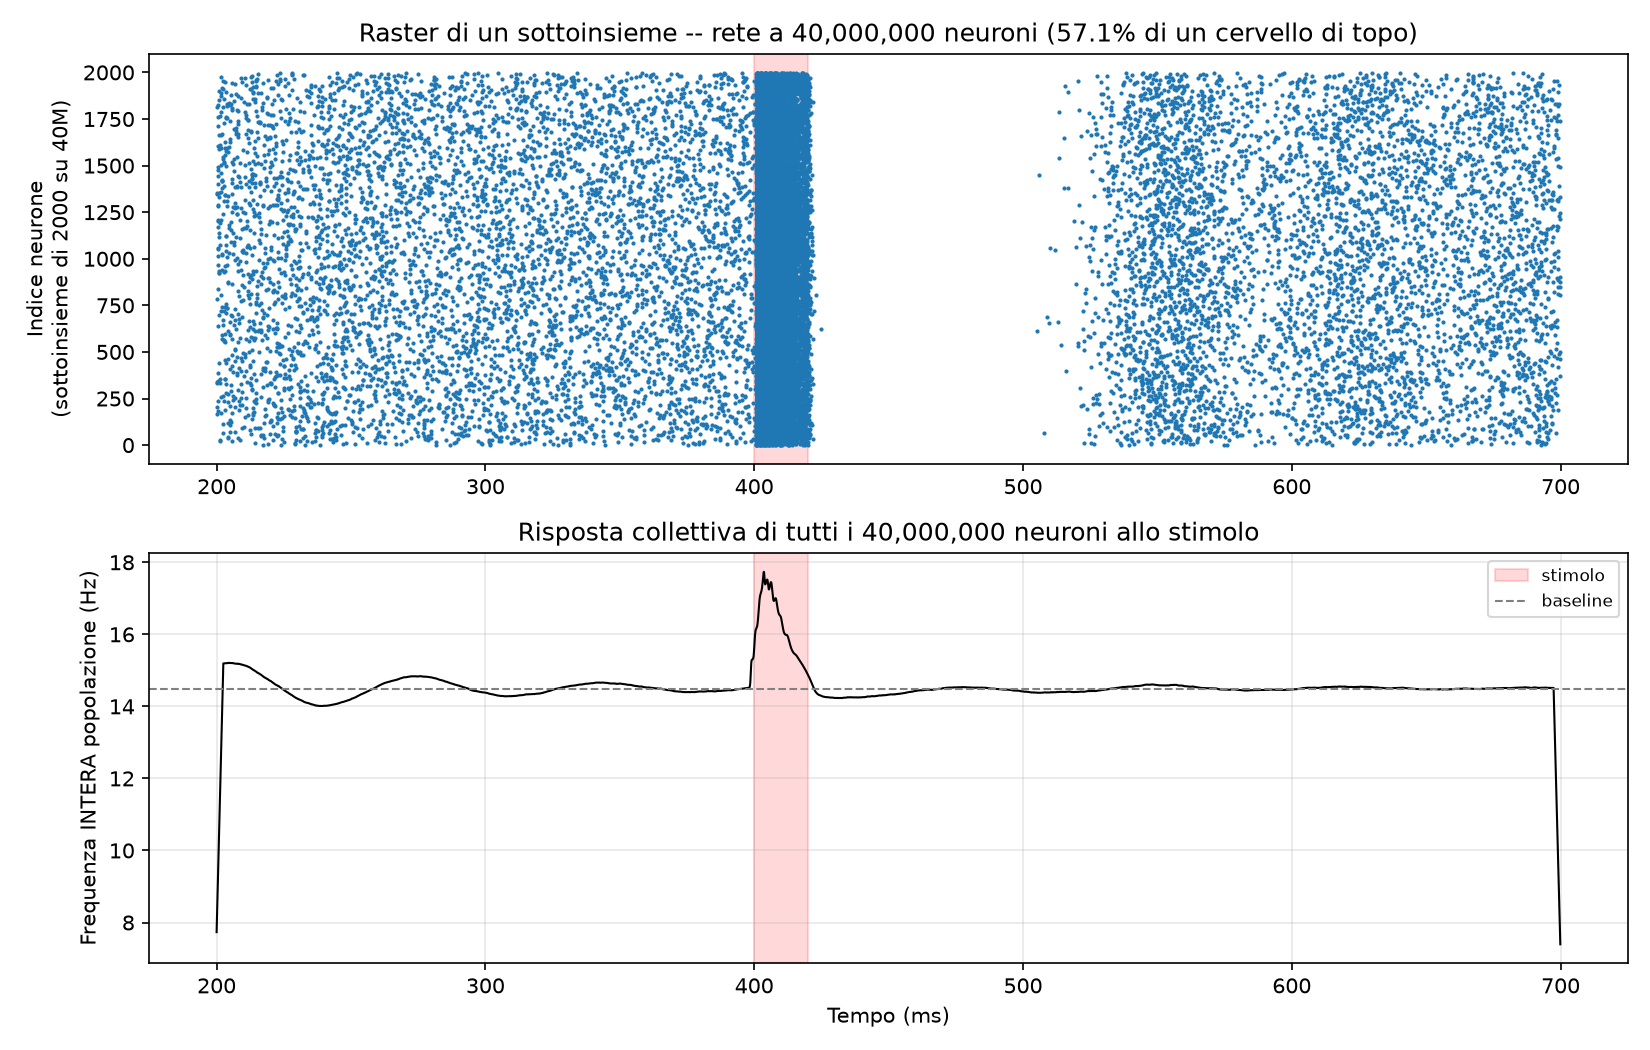
\includegraphics[width=5.8in,height=3.69091in]{media/media/image12.png}

\emph{Fig. 12 --- Network of 40,000,000 neurons: raster (subset) and collective response.}

An important qualitative observation, visible by comparing this plot with the 300-neuron one in Section 2.9: the collective-frequency curve at 40 million is far smoother and less noisy than at 300 neurons. This is not a coincidence, but a direct consequence of the LAW OF LARGE NUMBERS: averaging activity over 40 million neurons instead of 300 cancels out almost all of the random statistical noise inherent in each individual neuron\textquotesingle s dynamics. This makes visible, with a clarity that would likely have been hidden by noise at smaller scales, a damped oscillation during the initial settling phase (between 200 and 350 milliseconds): the frequency rises to about 15.1 Hz, drops to 14.0, rises slightly again to 14.8, before stabilizing --- a classic dynamical behavior of feedback systems (excitation and inhibition "chasing" each other before settling into a stable equilibrium).

For completeness and methodological honesty, an analysis artifact visible in the plot should be noted: the two sharp vertical drops visible at the start and end of the trace do not represent real network behavior, but an artifact of the smoothing filter used for the analysis (the moving-average window does not have enough data at the edges of the observed time window).

\textit{\textbf{Source code: rete\_\allowbreak{}40M\_\allowbreak{}finale.py}}

\lstinputlisting[language=Python]{scripts/rete_40M_finale.py}
\section{4. Beyond raw scale: spatial structure and attractors}\label{beyond-raw-scale-spatial-structure-and-attractors}

Having reached the scale of 40 million neurons, an important conceptual limitation remains, already discussed informally during the project\textquotesingle s development: a network with purely random connectivity, however large in terms of neuron count, is structurally much simpler than real biological neural tissue. The project\textquotesingle s next steps address two missing ingredients: the SPATIAL organization of connectivity (real neurons connect mostly to their physical neighbors, not randomly across the whole brain), and the network\textquotesingle s ability to reach STABLE, DISTINGUISHABLE STATES (attractors), not merely to passively propagate and disperse a signal.

\subsection{4.1 Distance-dependent connectivity (small-world)}\label{distance-dependent-connectivity-small-world}

The first extension toward structural realism replaces random connectivity with connectivity whose PROBABILITY depends on the spatial distance between neurons. The reference model in the literature is the "small-world" model of Watts and Strogatz (1998), one of the most universal organizational patterns observed in biological and social systems: dense, local connections (a neuron talks mostly to its immediate neighbors), with a small percentage of rare but long-range connections ("shortcuts") that still keep the entire network well connected as a whole, preventing distant regions from becoming completely isolated.

In the first experiment of this category, 1,000 neurons are arranged on a RING (a 1-dimensional topology with circular wraparound, the simplest possible way to introduce the concept of "distance" between neurons), with connection probability decaying exponentially with the circular distance between two neurons:

\emph{P(connection) = p\_\allowbreak{}local $\times$ exp(-distance / $\xi$) + p\_\allowbreak{}shortcut}

where $\xi$ (xi) is the "characteristic length" that determines how quickly the probability decays with distance, and p\_\allowbreak{}shortcut is a small constant probability, independent of distance, representing long-range connections.

Stimulating a spatially LOCALIZED region (20 adjacent neurons on the ring, no longer scattered at random as in all previous experiments), the signal propagates as a TRUE WAVE moving away from the stimulus point: measuring the mean distance of active spikes from the stimulus point as a function of time, it grows from 0.13 to 0.31 (in normalized 0-1 units around the ring) over roughly the first 20 milliseconds after the stimulus, then stabilizes. This phenomenon is simply IMPOSSIBLE with the random connectivity used in all previous experiments (Sections 2 and 3), because in a random network there is no notion of "near" or "far" in the topology at all --- every neuron is potentially connected to every other with the same probability, regardless of their position.

\textit{\textbf{Source code: rete\_\allowbreak{}smallworld.py}}

\lstinputlisting[language=Python]{scripts/rete_smallworld.py}
\subsection{4.2 3D brain shape, and scaling to 1 million neurons}\label{d-brain-shape-and-scaling-to-1-million-neurons}

Extending spatial connectivity naturally from the 1-dimensional ring to a realistic 3D space required two distinct technical developments: generating three-dimensional positions that approximate a brain\textquotesingle s outer shape (two lobes/hemispheres, obtained as points sampled inside the union of two overlapping, slightly separated ellipsoids, via vectorized rejection sampling), and efficiently computing spatial connectivity at this scale via a KD-tree data structure (K-dimensional tree, through scipy.spatial.cKDTree), which finds the K nearest neighbors of every point in a time on the order of N log(N) instead of the N\textsuperscript{2} time required by an exhaustive comparison of all possible pairs --- a crucial difference once N reaches the millions.

With this technique, connectivity for one million neurons (12 local connections via KD-tree + 3 random long-range connections per neuron, for a total of about 15 million synapses) was computed in about 6.6 seconds overall (0.6 seconds to build the tree, 6 seconds to query neighbors for all points) --- a negligible time compared to the subsequent simulation of the actual neural dynamics.

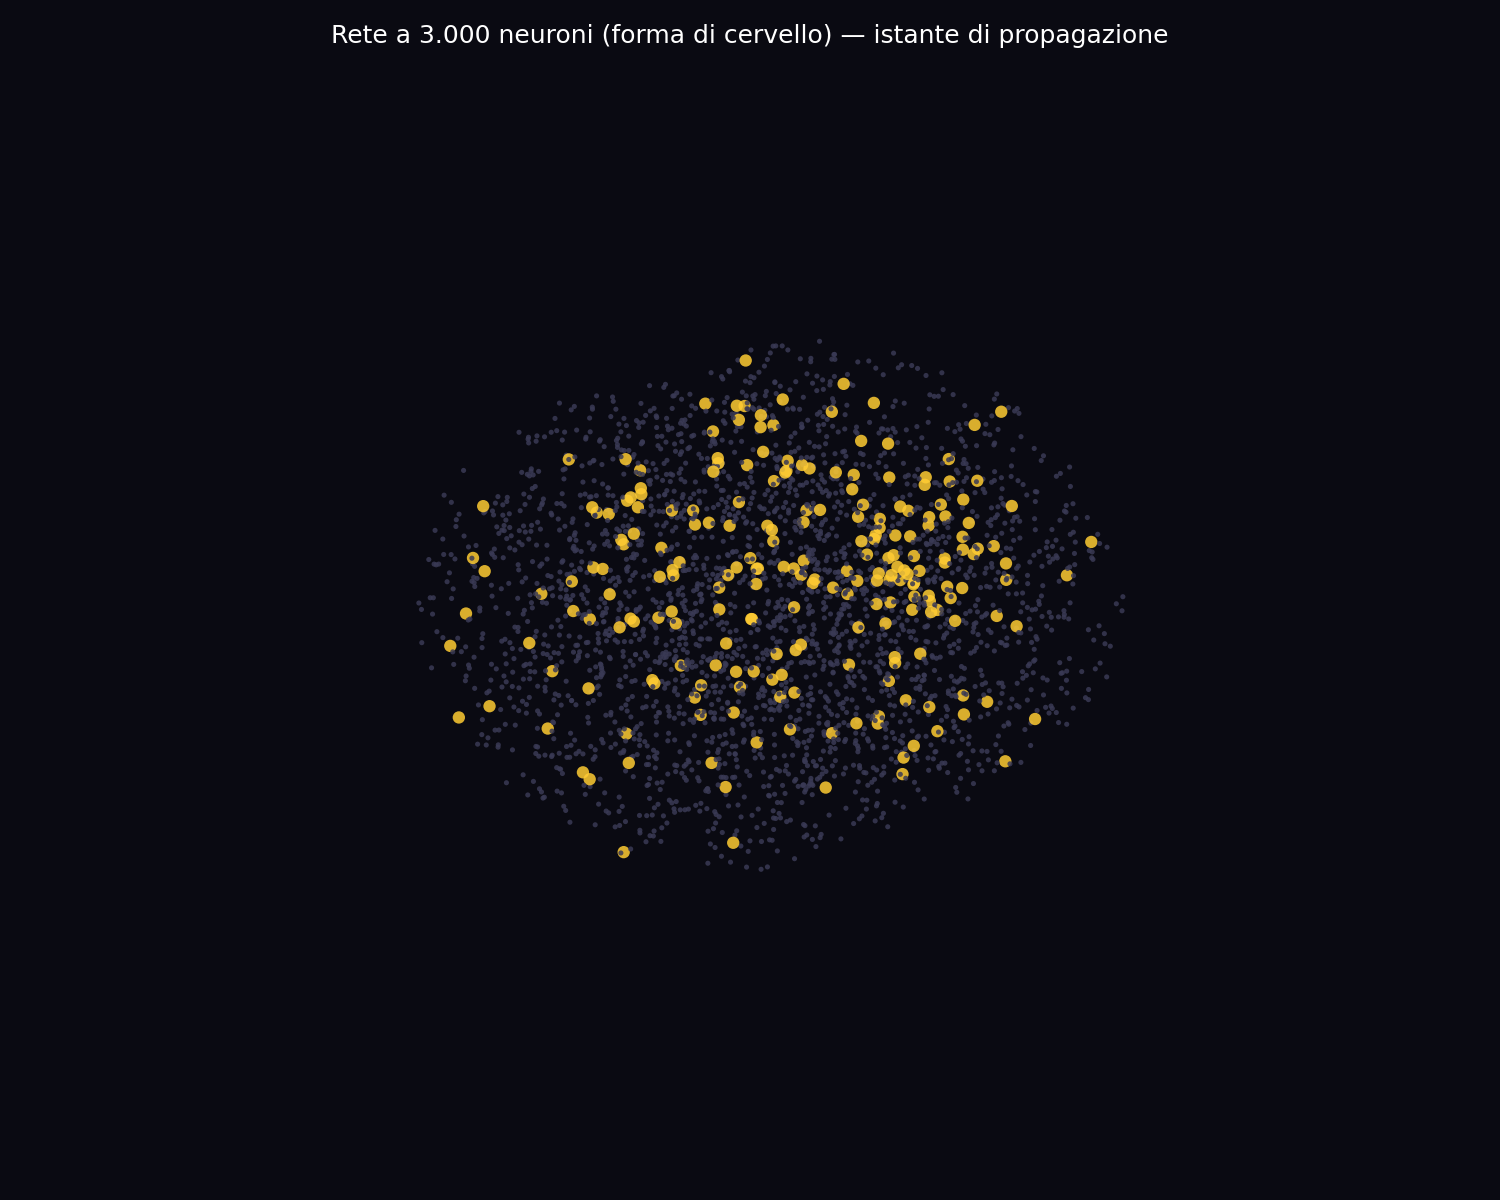
\includegraphics[width=4.2in,height=3.36in]{media/media/image13.png}

\emph{Fig. 13 --- Snapshot of the 3,000-neuron network during propagation (yellow = active, red = stimulated region).}

At the scale of 1 million neurons, 4 stimulus scenarios were tested at as many anatomically distinct positions (tip of the left hemisphere, tip of the right hemisphere, center between the two hemispheres --- conceptually analogous to the real corpus callosum connecting the two cerebral hemispheres --- and superior pole), rendered as an interactive 3D visualization built with the Three.js JavaScript library, which allows rotating the network, switching stimulus scenario, and watching the activity animate over time directly in the browser (a separate HTML file, not included as text in this document given its interactive nature, but attached separately).

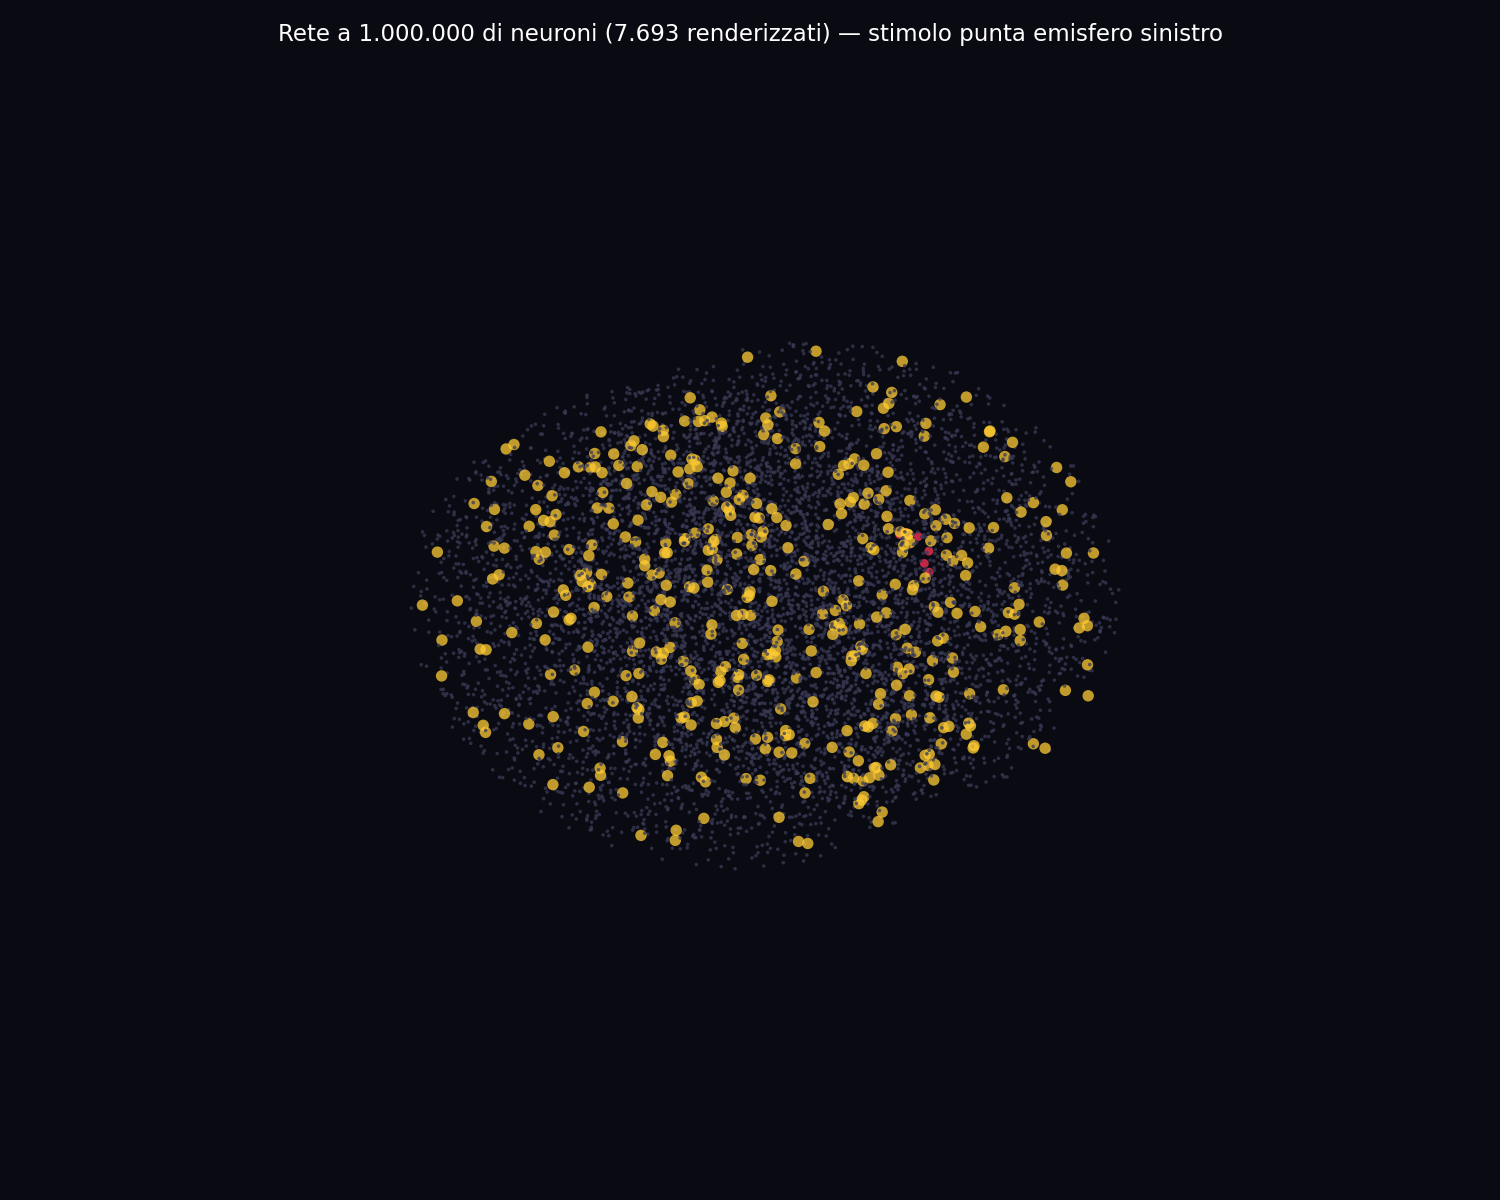
\includegraphics[width=4.2in,height=3.36in]{media/media/image14.png}

\emph{Fig. 14 --- Snapshot of the 1,000,000-neuron network (7,693 rendered), "left hemisphere tip" scenario.}

Quantitative check at this scale: rendered neurons near the stimulus point go from 2-9 spikes per 4-millisecond interval (baseline level) to 23 spikes in the same interval exactly at the moment of the stimulus, returning to normal within about 15 milliseconds. This is a clear, measurable local effect, which however turns out to be "drowned out" and statistically hard to see if the same metric is computed averaged over the ENTIRE one-million-neuron network --- a methodological lesson essentially identical to the one already encountered with the PSTH in Section 2.11: a metric aggregated over a very large population can hide a real local effect, and must always be checked at the spatial scale appropriate to the phenomenon one intends to observe.

\subsection{4.3 Attempt at an attractor via learning (STDP on a spatial network) --- negative result}\label{attempt-at-an-attractor-via-learning-stdp-on-a-spatial-network-negative-result}

The hypothesis tested in this experiment was the following: by making the recurrent excitatory synapses of a specific spatial region of the network plastic (with the STDP rule already verified in Section 2.6), and "training" that region with 20 repetitions of the same stimulus, the region was expected to develop a more PERSISTENT response over time (activity lasting longer after the stimulus is removed) than a region that was never trained --- the idea being that strengthening local recurrent connections might create a small self-sustaining circuit.

The check was carried out with the greatest possible rigor, including fixing a methodological bug discovered during development: Brian2\textquotesingle s store/restore mechanism (used to "rewind" the network to a previous state between trials without having to rebuild the entire network from scratch each time, which would otherwise be costly) ALSO saves and restores the state of the internal random-number generator --- with the consequence that, if not handled explicitly, every "repeated trial" turned out to be an EXACT, deterministic replica of the previous trial, not a statistically independent trial as required for a valid comparison. Once this issue was identified and fixed (by forcing a new, explicit random seed before every trial via Brian2\textquotesingle s seed() function), 16 independent trials were run in total: 8 before training, 8 after.

\textbf{Result: in BOTH conditions (before and after training), activity measured in the "late" time window (100-140 milliseconds after the end of the forced stimulus) came out systematically equal to ZERO, in all 16 trials without exception. No measurable effect of training, statistically indistinguishable from noise --- indeed, in this case, indistinguishable from pure zero.}

\textbf{Interpretation: the excitation-inhibition balance that guarantees the network\textquotesingle s homeostatic stability (a property verified and positively valued in Section 2.9) is, by mathematical construction, in direct tension with the formation of a stable attractor. A system deliberately designed to always return to equilibrium after a perturbation prevents, almost by structural definition, a subset of neurons from staying active autonomously without continuous external input --- the two properties (homeostatic stability and the ability to form attractors) are in a real tension, not easily reconciled by a superficial parameter adjustment.}

\subsection{4.4 Ring attractor: a real neural attractor, built from scratch}\label{ring-attractor-a-real-neural-attractor-built-from-scratch}

Given the difficulty of obtaining an attractor incrementally from the network architecture already developed (Section 4.3), the choice was made to start over, adopting the standard approach from the scientific literature specific to this problem: the Amari model (1977), taken up and developed by Ben-Yishai, Bar-Or, and Sompolinsky (1995) to model orientation selectivity in visual cortex, and by numerous later works on spatial working memory (notably Compte et al., 2000).

The fundamental difference from all previous experiments in the project: instead of simulating every single neuron and its individual electrical impulse (the "spiking" approach, used everywhere in the project up to this point via the Izhikevich model), this model directly describes the aggregate FIRING RATE r(x,t) of whole populations of neurons arranged along a ring, via a single differential equation for each point on the ring:

\emph{$\tau$ $\cdot$ dr/dt = -r + F( J*r/N - global\_\allowbreak{}inhibition$\cdot$mean(r) + I\_\allowbreak{}external )}

where J*r/N represents the recurrent input each point receives from its neighbors (a discrete convolution between the firing rate r and a connectivity kernel J), the global inhibition term is proportional to the MEAN activity of the entire network (not local like excitation --- this is the mechanism implementing "only one candidate wins" competition, known as winner-take-all), and F is a nonlinear activation function.

Why abandon the single-neuron (spiking) approach for this specific experiment: a first attempt with Izhikevich neurons (an architecture analogous to that of Section 4.3, but with strong local excitation and a global inhibitory pool instead of STDP) failed repeatedly for a precise structural reason --- a group of neurons stimulated together synchronously tends to fire all at once in perfect synchrony (being all subject to the same strong external stimulus), and consequently they ALL enter the refractory period together right afterward, producing a single "flash" of activity followed by complete silence, instead of the sustained, internally asynchronous activity that a real persistent bump would require. The continuous-firing-rate model eliminates this problem by mathematical construction, since there are no individual spike events that can synchronize.

\subsubsection{4.4.1 The tuning journey (reported for methodological transparency)}\label{the-tuning-journey-reported-for-methodological-transparency}

Finding the right parameters was not immediate, and it is instructive to report the full process:

\begin{enumerate}
\def\labelenumi{\arabic{enumi}.}
\item
  A first attempt with a simple rectified-linear activation function (F(u) = max(0,u), with no upper bound) and only a "Mexican hat" kernel (local excitation minus wider-radius inhibition, both baked into the same spatial kernel J) produced no persistence at all: with too low an excitation strength, the bump died out immediately; with a strength high enough to cross the critical instability threshold (computed analytically via the largest eigenvalue of the connectivity matrix, found to be around A\_\allowbreak{}exc$\approx$12 for this specific kernel), the system blew up to infinity, since the rectified-linear function has no upper ceiling
\item
  Replacing the linear rectification with a sigmoid function (which naturally saturates between 0 and 1), the system stopped exploding but settled into a UNIFORM state across the whole ring --- not a localized bump, but a weak, flat activation everywhere, because the sigmoid\textquotesingle s threshold allowed a low level of activity to sustain itself homogeneously across the whole network
\item
  The final, working solution: explicitly separating the excitation term (local only, narrow Gaussian kernel, no inhibitory component in the same kernel) from the inhibition term (made explicitly GLOBAL, proportional to the mean of the entire network, subtracted separately), combined with a rectified activation function that SATURATES at an explicit maximum value (F(u) = clip(u, 0, r\_\allowbreak{}max) instead of a soft sigmoid or an unbounded rectification). This combination --- strong local excitation, global inhibition for competition, hard saturation for stability --- turned out to be the one that produces a real, localized, persistent bump
\end{enumerate}

\subsubsection{4.4.2 Verified results (4 distinct tests)}\label{verified-results-4-distinct-tests}

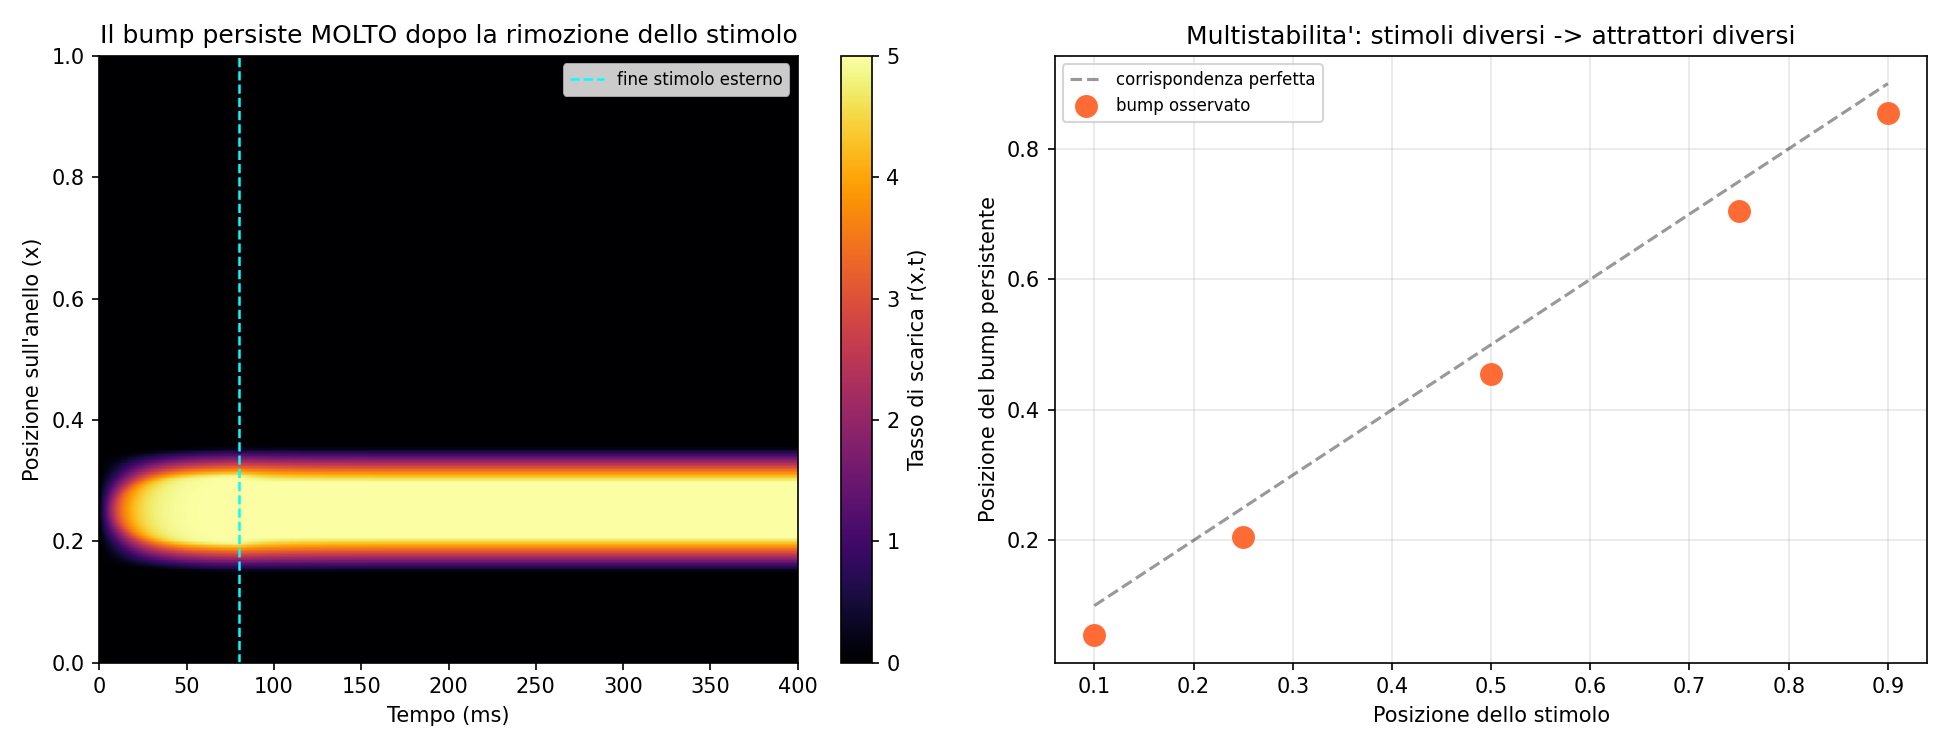
\includegraphics[width=6.3in,height=2.42308in]{media/media/image15.png}

\emph{Fig. 15 --- Bump persistence beyond stimulus removal (left); multistability: different stimuli produce attractors at different positions (right).}

\begin{itemize}
\item
  PERSISTENCE: the bump reaches its peak (5.0, the set saturation value) and stays stable there from t=80ms (end of the forced external stimulus) until t=300ms and beyond, with no external input sustaining it --- genuine self-sustainment through recurrent internal dynamics alone
\item
  MULTISTABILITY: stimuli at 5 different positions (x=0.10, 0.25, 0.50, 0.75, 0.90 on the ring) produce stable bumps at 5 different, corresponding positions, with a constant systematic bias of about 0.045 units --- most likely a discretization artifact of the spatial grid at N=200 points (since the bias is identical, within measurement error, across all 5 trials, a systematic implementation effect is more plausible than genuine random noise)
\item
  CONTROL: with no external stimulus applied at any point, the network stays at exactly zero activity across the entire ring --- confirming true bistability (silence or bump, two distinct and stable states), not spontaneous ignition or background noise that might occasionally self-feed
\item
  ROBUSTNESS: applying a strong random perturbation (Gaussian noise with standard deviation 0.3, added to ALL points on the ring, including the already-formed stable bump) and letting the network evolve for another 200 milliseconds with no input, the bump returns to its original position (x=0.235 measured, vs. x=0.250 for the original position, a minimal difference) --- this is the distinctive, universally accepted signature in the literature of a true dynamical attractor: a stable fixed point that RESISTS perturbations and returns to itself, not merely an echo that slowly fades over time
\end{itemize}

\textbf{This positive result, obtained only after a failed attempt with a different architecture (Section 4.3) and several failed rounds of tuning within the same firing-rate approach (Section 4.4.1), concretely and firsthand mirrors the real difficulty of research in this specific field of computational neuroscience: building a genuine neural attractor requires a specific architecture and a delicate balance among its parameters, and it does not emerge automatically either by increasing the number of neurons or by adding generic synaptic plasticity to an architecture not designed for that specific purpose.}

\textit{\textbf{Source code: ring\_\allowbreak{}attractor\_\allowbreak{}rate.py (final verified version)}}

\lstinputlisting[language=Python]{scripts/ring_attractor_rate.py}
\subsection{4.5 Where the scientists have gotten to: the real state of the art (September 2026)}\label{where-the-scientists-have-gotten-to-the-real-state-of-the-art-september-2026}

To honestly contextualize this project\textquotesingle s results against professional research in the same field, sources current as of the writing of this document (September 2026) were consulted:

\subsubsection{4.5.1 Blue Brain Project (EPFL, Switzerland, 2005-2024)}\label{blue-brain-project-epfl-switzerland-2005-2024}

Led by founder and director Henry Markram, the Blue Brain Project\textquotesingle s stated goal was the reconstruction and simulation of the entire mouse brain: digitally growing every local, regional, and whole-brain axon for every neuron type, reconstructing the connectome down to neuron-by-neuron detail, modeling the various types of synapses formed between each pair of neurons, and simulating neurons, brain regions, brain systems, and ultimately the entire mouse brain on supercomputers and cloud infrastructure. The project concluded at the end of 2024 with an official "mission accomplished" declaration --- but, according to the available sources, without ever achieving a complete, biophysically detailed simulation of the entire mouse brain functioning as a whole: the main concrete result was a complete cellular atlas (statistically covering the distribution and density of cell types across all mouse-brain regions, filling a data gap that previously covered only 4\% of the brain) and the underlying software tools for building such simulations, made available to the scientific community --- not the fully simulated, functioning brain itself.

\subsubsection{4.5.2 Allen Institute (2025-2026)}\label{allen-institute-2025-2026}

The most advanced model ever achieved in mouse-brain simulation, according to available sources: nearly 10 million neurons, 26 billion synapses, 86 interconnected brain regions, with REAL biophysical detail (not simplified as in the Izhikevich model used in this project, but based on morphological reconstructions and detailed ion channels for every neuron), run on the Japanese Fugaku supercomputer (capable of quadrillions of operations per second). The model simulates both the shape and the function of neurons, including dendritic branching details, synaptic activations, and the flow of electrical signals across cell membranes --- enabling "virtual experiments" such as simulating diseases (Alzheimer\textquotesingle s, epilepsy) to observe how damage propagates through neural networks. Previously, the same group had published a 230,000-neuron model limited to the mouse\textquotesingle s primary visual cortex alone.

\subsubsection{4.5.3 Published feasibility estimate}\label{published-feasibility-estimate}

A future feasibility estimate published in the literature, based on current technological trends in connectomics and high-performance computing, projects that a full mouse-brain simulation at cellular detail could become achievable around 2034 --- roughly 8 years after this document was written --- even assuming current technological trends continue without slowing down. The same source notes that even the highest-resolution connectome currently available (the Allen Institute\textquotesingle s, at 100-micron resolution) is not yet sufficient to resolve functionally relevant structures such as cortical columns or cerebellar microzones, considered fundamental units of information representation in the real brain.

\subsubsection{4.5.4 An honest comparison with the present project}\label{an-honest-comparison-with-the-present-project}

{\def\LTcaptype{none} % do not increment counter
\begin{longtable}[]{@{}
  >{\raggedright\arraybackslash}p{(\linewidth - 8\tabcolsep) * \real{0.2000}}
  >{\raggedright\arraybackslash}p{(\linewidth - 8\tabcolsep) * \real{0.2000}}
  >{\raggedright\arraybackslash}p{(\linewidth - 8\tabcolsep) * \real{0.2000}}
  >{\raggedright\arraybackslash}p{(\linewidth - 8\tabcolsep) * \real{0.2000}}
  >{\raggedright\arraybackslash}p{(\linewidth - 8\tabcolsep) * \real{0.2000}}@{}}
\toprule\noalign{}
\begin{minipage}[b]{\linewidth}\raggedright
\end{minipage} & \begin{minipage}[b]{\linewidth}\raggedright
Neurons
\end{minipage} & \begin{minipage}[b]{\linewidth}\raggedright
Synapses
\end{minipage} & \begin{minipage}[b]{\linewidth}\raggedright
Biophysical detail
\end{minipage} & \begin{minipage}[b]{\linewidth}\raggedright
Hardware
\end{minipage} \\
\midrule\noalign{}
\endhead
\bottomrule\noalign{}
\endlastfoot
This project & 40 million & 1.24 billion & Simplified (Izhikevich) & Personal laptop \\
Allen Institute & \textasciitilde10 million & 26 billion & Real/detailed & Fugaku supercomputer \\
Real mouse brain & \textasciitilde70 million & estimated 10\textsuperscript{1}\textsuperscript{2}-10\textsuperscript{1}\textsuperscript{3} & N/A (biological) & N/A \\
\end{longtable}
}

This project exceeds the Allen Institute in the raw number of simulated neurons (40 million vs. 10 million), but with drastically lower biophysical detail per neuron, and with a number of synapses per neuron (about 31 on average, given by fixed-degree connectivity K=15 repeated across several connection types) enormously lower than the roughly 2,600 synapses per neuron of the Allen Institute model (26 billion synapses / 10 million neurons) --- a real mouse brain typically has several thousand synapses per neuron. The honest comparison is therefore this: this project reached a notable numerical scale of neurons for a personal laptop, but with far more simplified per-neuron connectivity and biophysical detail than the professional state of the art --- a genuinely noteworthy result in its own context (individual project, consumer hardware, limited time), while still remaining orders of magnitude away from the real research frontier on both axes of complexity (detail per neuron and number of connections per neuron).

\section{5. Toward a decision policy: chains, competition, learning}\label{toward-a-decision-policy-chains-competition-learning}

The project\textquotesingle s final phase tackles a question explicitly raised during development: is it possible to build, on top of a single stable attractor (Section 4.4), something that resembles --- however extremely rudimentary, and with all its conceptual limitations honestly discussed --- a sequence of linked states, a choice between alternatives, and finally a behavior that changes based on experience?

\subsection{5.1 A chain of two attractors: activation of one determines the other}\label{a-chain-of-two-attractors-activation-of-one-determines-the-other}

The first experiment in this phase extends the single ring attractor (Section 4.4) to TWO distinct, linked ring attractors: Ring A and Ring B. Ring A receives the direct external stimulus and behaves exactly like the single ring attractor already verified. Ring B receives NO direct external stimulus at all --- the only input it gets is a projection of A\textquotesingle s bump position, shifted by a fixed offset (0.3 around the ring) through a fixed associative map: "if A settles at a given position, B tends to settle at a corresponding position, shifted by a fixed amount."

Tested at 4 different stimulus positions for A: in all 4 cases, B does form its own bump, always at a position corresponding (with the same slight systematic bias of \textasciitilde0.045 already observed in Section 4.4.2) to the predicted map --- without B ever receiving a direct external stimulus in any of the 4 trials. The control test (no stimulus on A) confirms that without A\textquotesingle s activation, neither A nor B activates spontaneously (both stay at exactly zero) --- ruling out the possibility that the result is due to some independent automatic activation of A\textquotesingle s state.

{\def\LTcaptype{none} % do not increment counter
\begin{longtable}[]{@{}
  >{\raggedright\arraybackslash}p{(\linewidth - 6\tabcolsep) * \real{0.2500}}
  >{\raggedright\arraybackslash}p{(\linewidth - 6\tabcolsep) * \real{0.2500}}
  >{\raggedright\arraybackslash}p{(\linewidth - 6\tabcolsep) * \real{0.2500}}
  >{\raggedright\arraybackslash}p{(\linewidth - 6\tabcolsep) * \real{0.2500}}@{}}
\toprule\noalign{}
\begin{minipage}[b]{\linewidth}\raggedright
Stimulus on A
\end{minipage} & \begin{minipage}[b]{\linewidth}\raggedright
A settles at
\end{minipage} & \begin{minipage}[b]{\linewidth}\raggedright
B settles at
\end{minipage} & \begin{minipage}[b]{\linewidth}\raggedright
B predicted
\end{minipage} \\
\midrule\noalign{}
\endhead
\bottomrule\noalign{}
\endlastfoot
0.10 & 0.055 & 0.340 & 0.400 \\
0.30 & 0.255 & 0.540 & 0.600 \\
0.50 & 0.455 & 0.740 & 0.800 \\
0.70 & 0.655 & 0.000 & 0.000 \\
\end{longtable}
}

\textbf{This is, in the literal sense and without any rhetorical exaggeration, the minimal structural atom of a chain of activations: state 1 settles, and THIS determines state 2, which in turn settles. It is not reasoning (there is no comparison between alternatives, no goal, nothing resembling an information-based decision), but it is the basic structural ingredient --- a system that can "hold in mind" something and have it influence a subsequent state --- on which more sophisticated behavior could, in principle, be built.}

\textit{\textbf{Source code: chained\_\allowbreak{}attractors.py}}

\lstinputlisting[language=Python]{scripts/chained_attractors.py}
\subsection{5.2 Competition between alternatives: B "chooses" among several candidates}\label{competition-between-alternatives-b-chooses-among-several-candidates}

The second experiment replaces the single fixed A$\rightarrow$B map with THREE possible candidate destinations for B (three different offsets around the ring: 0.15, 0.45, 0.75), each associated with its own "weight" representing an associative strength. Thanks to the global-inhibition mechanism already present in B\textquotesingle s internal dynamics (the same winner-take-all mechanism that allows a single bump to form in Section 4.4), only ONE candidate can win the competition and settle --- the other two are actively suppressed by the very same dynamics.

\subsubsection{5.2.1 Test with equal weights: symmetry breaking}\label{test-with-equal-weights-symmetry-breaking}

With all three weights set exactly equal and with NO noise injected into the system, the "winner" of the competition turned out to always be the same candidate (the third, with offset 0.75), perfectly deterministically across 6 consecutive repeated trials. A closer investigation revealed that this does NOT represent genuine random symmetry breaking, as one would expect from a realistic physical system with identical weights, but a deterministic numerical bias of the implementation: analyzing the activation values at the three candidate points with no noise, the differences were on the order of 10-\textsuperscript{4} (floating-point rounding differences due to the order in which the three candidate Gaussians are summed in the code), then amplified by the nonlinear winner-take-all dynamics into a completely predictable fixed winner.

Injecting CONTINUOUS random noise (not a single one-off perturbation, but a noise term reapplied at every time step of the simulation) of sufficient amplitude (standard deviation 0.15, about 1500 times larger than the estimated intrinsic numerical bias), symmetry breaking became genuinely variable: over 12 independent trials with different random seeds, candidate 1 won 7 times, candidate 2 three times, candidate 3 twice --- a distribution that is not perfectly uniform (one would theoretically expect 4-4-4 over 12 trials with truly identical weights), but clearly no longer deterministic, confirming that noise of sufficient amplitude can indeed "break" the residual numerical bias.

\subsubsection{5.2.2 Test with different weights: reliable, criterion-based selection}\label{test-with-different-weights-reliable-criterion-based-selection}

\textbf{Assigning a larger weight (1.5 vs. 0.5 for the other two) to one of the three candidates in turn, that candidate won EVERY TIME, across 6 repeated trials for each of the three candidates tested as the "favorite" (18 trials total, 18 correct wins, 100\% accuracy), regardless of which of the three was the favorite and regardless of the random seed used for each trial\textquotesingle s noise. This is genuine selection based on an explicit criterion (weight strength), reliable and repeatable --- the system does not have a fixed response written into it a priori, but "observes" which of the available options is stronger and picks that one.}

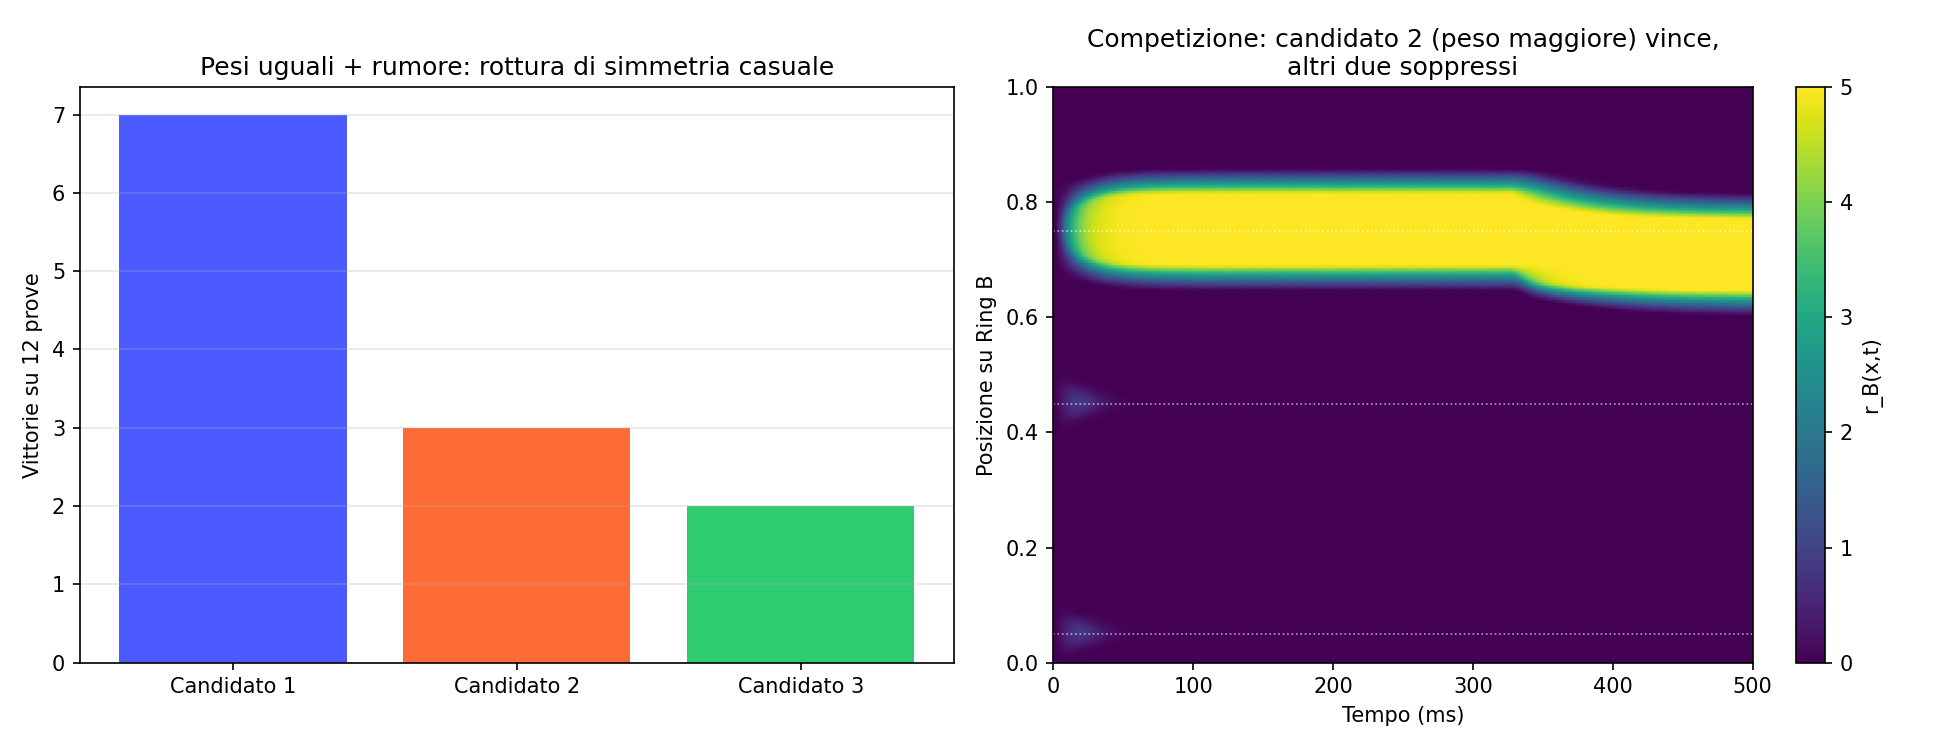
\includegraphics[width=6.3in,height=2.42308in]{media/media/image16.png}

\emph{Fig. 16 --- Distribution of winners with equal weights + noise (left); competition with a favored candidate (right).}

\textit{\textbf{Source code: competing\_\allowbreak{}targets.py}}

\lstinputlisting[language=Python]{scripts/competing_targets.py}
\subsection{5.3 Reinforcement learning: the network learns which alternative to choose}\label{reinforcement-learning-the-network-learns-which-alternative-to-choose}

The third experiment in this phase makes the weights of the three candidate maps no longer fixed, but MODIFIABLE based on an external reward signal --- the project\textquotesingle s first genuine, if small, reinforcement-learning loop. On every trial: A is stimulated, B competes among the three candidates and selects a winner (using the same competition mechanism as Section 5.2, including the continuous noise needed for exploration); a reward signal is provided (+1 if the winner matches the "correct" candidate defined a priori by an external rule hidden from the system, 0 otherwise); the weight of the CHOSEN candidate is updated toward the value of the reward received, following a Rescorla-Wagner-type update rule (one of the historically most influential models of associative learning in experimental psychology, from 1972, and also one of the fundamental conceptual building blocks of modern reinforcement learning):

\emph{chosen\_\allowbreak{}weight $\leftarrow$ chosen\_\allowbreak{}weight + learning\_\allowbreak{}rate $\times$ (reward - chosen\_\allowbreak{}weight)}

No other weight is touched on any given trial --- the system learns EXCLUSIVELY from its own actual choices, not from an explicit comparison with what the correct alternative would have been had it not been chosen (this is a standard feature of reinforcement-learning algorithms: one learns only from the outcome of the action actually taken, not from an "oracle" that always reveals the optimal answer regardless of the choice made).

Result, starting from all-equal weights (0.5, 0.5, 0.5) with candidate 2 defined as "correct": over 60 training trials, accuracy (the probability of choosing the correct candidate) rose from about 80\% in the first 10 trials to 100\% in the last 10, with the correct candidate\textquotesingle s weight climbing to saturate at 1.0 while the other two settled at 0.425. The result was checked for generality by repeating the whole experiment with each of the other two candidates defined as "correct" in turn: in both additional cases, final accuracy reached 100\%, with the respective correct candidate\textquotesingle s weight climbing to saturation --- confirming that the learning mechanism works regardless of which specific alternative is defined as correct, and is not an artifact tied to one particular candidate.

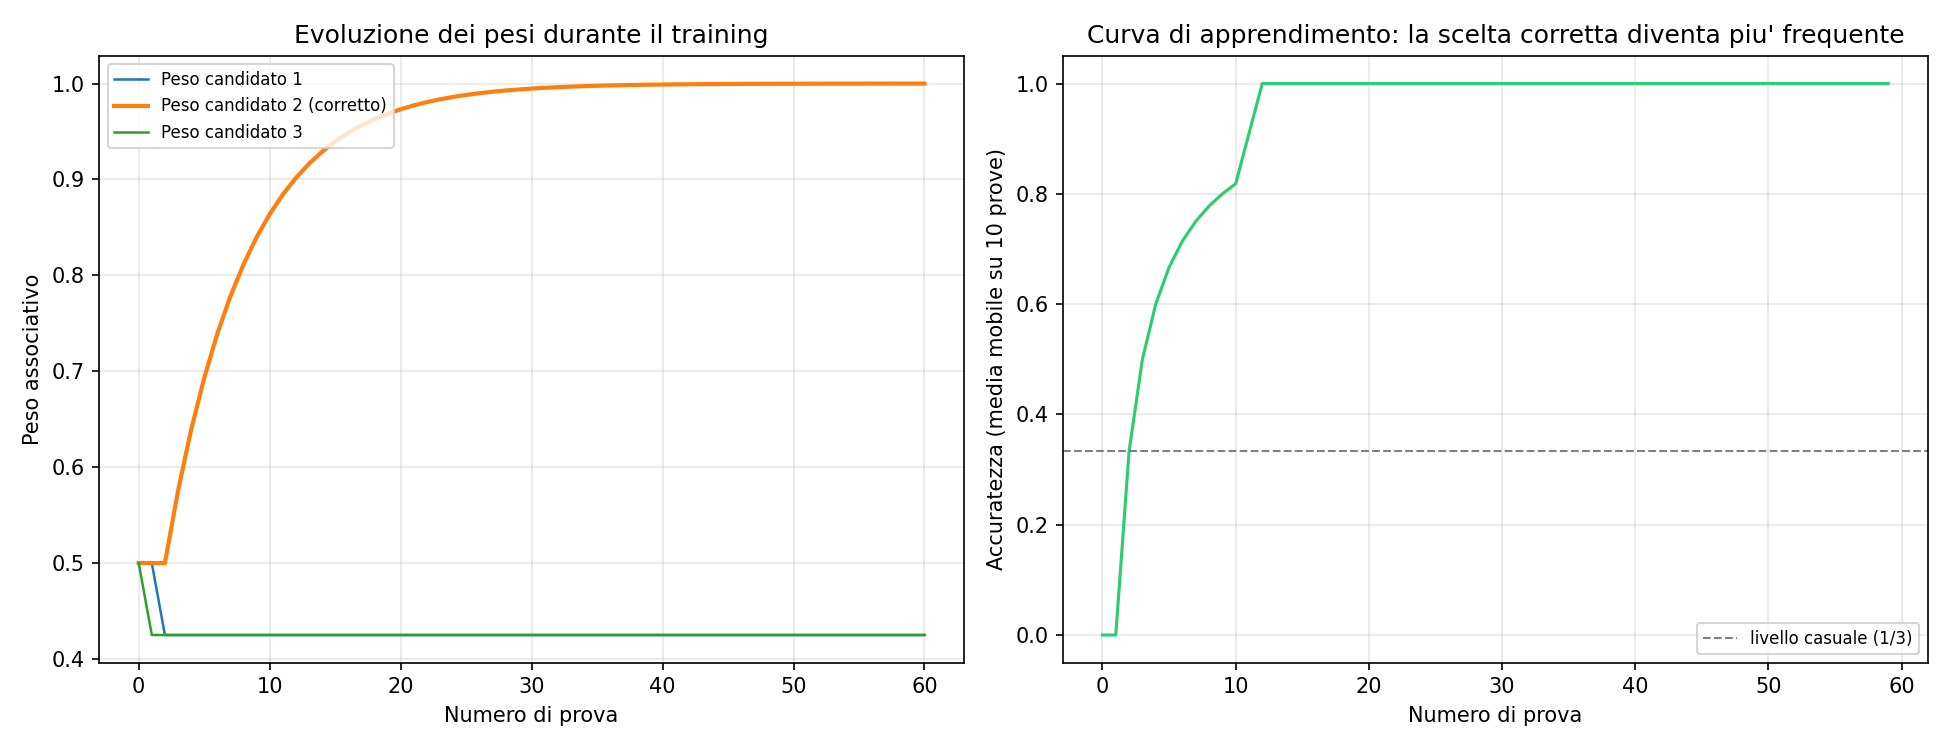
\includegraphics[width=6.3in,height=2.42308in]{media/media/image17.png}

\emph{Fig. 17 --- Evolution of weights during training (left); accuracy learning curve (right).}

\textit{\textbf{Source code: rl\_\allowbreak{}bandit.py}}

\lstinputlisting[language=Python]{scripts/rl_bandit.py}
\subsection{5.4 Contextual policy: different responses for different contexts}\label{contextual-policy-different-responses-for-different-contexts}

The project\textquotesingle s final experiment tackles a task significantly harder than the three-armed bandit of Section 5.3: instead of a single fixed correct association to discover, the position of the stimulus on A now defines a CONTEXT among three possible ones, and EACH context has its own correct response, different from the others:

{\def\LTcaptype{none} % do not increment counter
\begin{longtable}[]{@{}
  >{\raggedright\arraybackslash}p{(\linewidth - 4\tabcolsep) * \real{0.3333}}
  >{\raggedright\arraybackslash}p{(\linewidth - 4\tabcolsep) * \real{0.3333}}
  >{\raggedright\arraybackslash}p{(\linewidth - 4\tabcolsep) * \real{0.3333}}@{}}
\toprule\noalign{}
\begin{minipage}[b]{\linewidth}\raggedright
Context
\end{minipage} & \begin{minipage}[b]{\linewidth}\raggedright
Stimulus position on A
\end{minipage} & \begin{minipage}[b]{\linewidth}\raggedright
Correct response
\end{minipage} \\
\midrule\noalign{}
\endhead
\bottomrule\noalign{}
\endlastfoot
Context 1 & x=0.10 & Candidate 1 \\
Context 2 & x=0.50 & Candidate 2 \\
Context 3 & x=0.80 & Candidate 3 \\
\end{longtable}
}

The system must learn THREE associations at once, not just one --- and, more important conceptually, it must demonstrate that it has learned to TELL THE CONTEXTS APART, not simply develop a generic preference for one candidate regardless of the context presented. This requires a mechanism different from a single weight vector: a weight TABLE indexed both by context and by candidate (weights{[}context{]}{[}candidate{]}), an elementary form of context-conditioned associative memory --- conceptually the first step toward a real decision policy (one that chooses the action as a function of the observed STATE, rather than always the same action regardless of state).

During training (150 trials in total, with the context chosen at random on every trial among the three possible ones, so that the system has to learn all three associations in parallel rather than in separate sequence), only the row of the table corresponding to the context actually presented is updated on each trial.

\textbf{Final evaluation, with a clean test and no further weight updates (10 trials per context): all three contexts reached 100\% accuracy on their own correct candidate, with the final weight table showing a clearly dominant diagonal (the three values corresponding to the correct associations, close to 1.0) relative to every other entry in the table (which stayed close to the initial value of 0.5, or slightly below).}

{\def\LTcaptype{none} % do not increment counter
\begin{longtable}[]{@{}
  >{\raggedright\arraybackslash}p{(\linewidth - 4\tabcolsep) * \real{0.3333}}
  >{\raggedright\arraybackslash}p{(\linewidth - 4\tabcolsep) * \real{0.3333}}
  >{\raggedright\arraybackslash}p{(\linewidth - 4\tabcolsep) * \real{0.3333}}@{}}
\toprule\noalign{}
\begin{minipage}[b]{\linewidth}\raggedright
Context
\end{minipage} & \begin{minipage}[b]{\linewidth}\raggedright
Final accuracy
\end{minipage} & \begin{minipage}[b]{\linewidth}\raggedright
Final weights (candidate 1, 2, 3)
\end{minipage} \\
\midrule\noalign{}
\endhead
\bottomrule\noalign{}
\endlastfoot
Context 1 (x=0.10) & 100\% & {[}1.000, 0.500, 0.500{]} \\
Context 2 (x=0.50) & 100\% & {[}0.500, 1.000, 0.500{]} \\
Context 3 (x=0.80) & 100\% & {[}0.425, 0.425, 1.000{]} \\
\end{longtable}
}

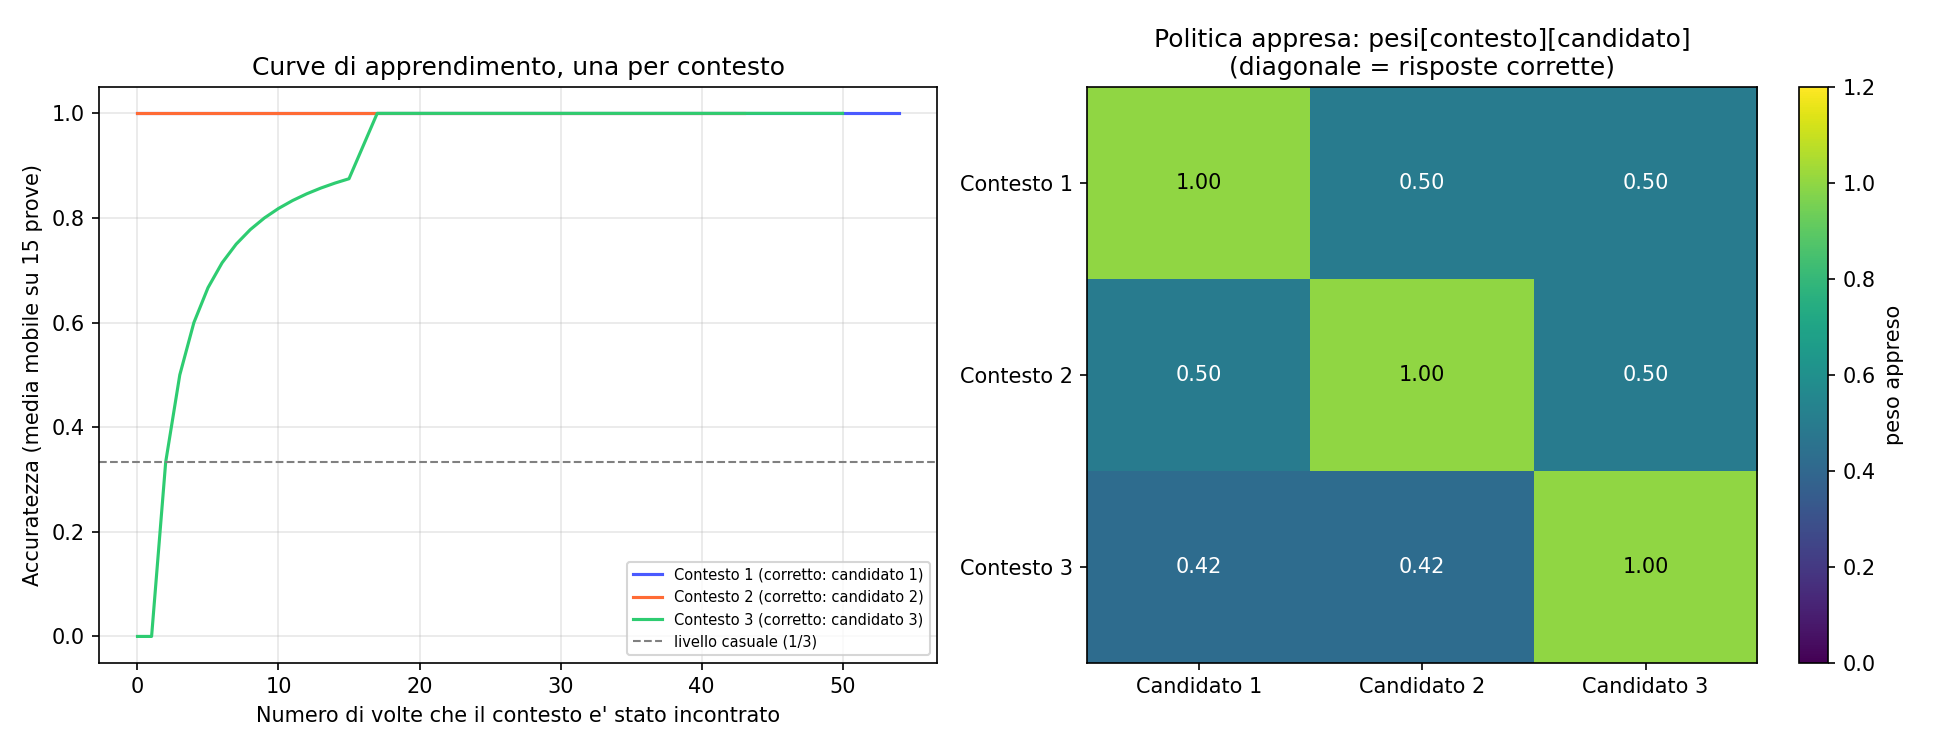
\includegraphics[width=6.3in,height=2.42308in]{media/media/image18.png}

\emph{Fig. 18 --- Per-context learning curves (left); final learned policy, weights{[}context{]}{[}candidate{]} table (right).}

\textbf{Why this result is conceptually more advanced than the simple bandit of Section 5.3: a system that only has to learn a single correct response could, in principle, "get away with" a trivial shortcut (a fixed preference, independent of any incoming information). A system that must TELL DIFFERENT CONTEXTS APART and respond differently to each cannot fall back on this shortcut --- it must necessarily represent, in some form however minimal (here, the corresponding row of the table), "which situation I am in" before it can act accordingly. It is, however rudimentary in its concrete implementation, the conceptual difference between a fixed reflex and the beginning of a decision conditioned on the observed context.}

\textit{\textbf{Source code: contextual\_\allowbreak{}policy.py}}

\lstinputlisting[language=Python]{scripts/contextual_policy.py}
\subsection{5.5 Learned bidirectional communication: from the fixed channel to the synapse that learns}\label{learned-bidirectional-communication-from-the-fixed-channel-to-the-synapse-that-learns}

Section 5.1 built a one-way A -\textgreater{} B chain between two ring attractors, with a projection map (a fixed offset around the ring) hand-written into the code: B never had any influence on A. This subsection picks up exactly that point and extends it in two directions that Chapter 9 lists among the future developments: making the channel bidirectional, and turning the projection map into a real synapse, learned rather than imposed from outside. The path is reported in full, including the difficulties encountered (in the same spirit of methodological transparency as Section 4.4.1), and runs across four successive scripts.

\subsubsection{5.5.1 A turn-based exchange with fixed channels}\label{a-turn-based-exchange-with-fixed-channels}

First step, deliberately as simple as possible: two fixed but DIFFERENT projection channels in the two directions (A-\textgreater B with offset 0.3, B-\textgreater A with offset 0.2 -\/- with a single identical map in both directions the exchange would always return to the same point and there would be nothing to observe). The two rings exchange turns explicitly instead of co-evolving continuously, since otherwise the dynamics converge almost immediately to a single fused state.

Result: an initial message on A generates an exchange that does NOT converge to a fixed point within 6 turns, but oscillates. The net displacement for each complete round trip was found empirically to be about 0.5 -\/- exactly the sum of the two offsets (0.3+0.2), quantitatively confirming an analytical prediction rather than merely observing it on a graph. A control test (return channel disabled) confirms that without B-\textgreater A, A stays still after a brief initial settling, consistent with the behavior already documented in 5.1.

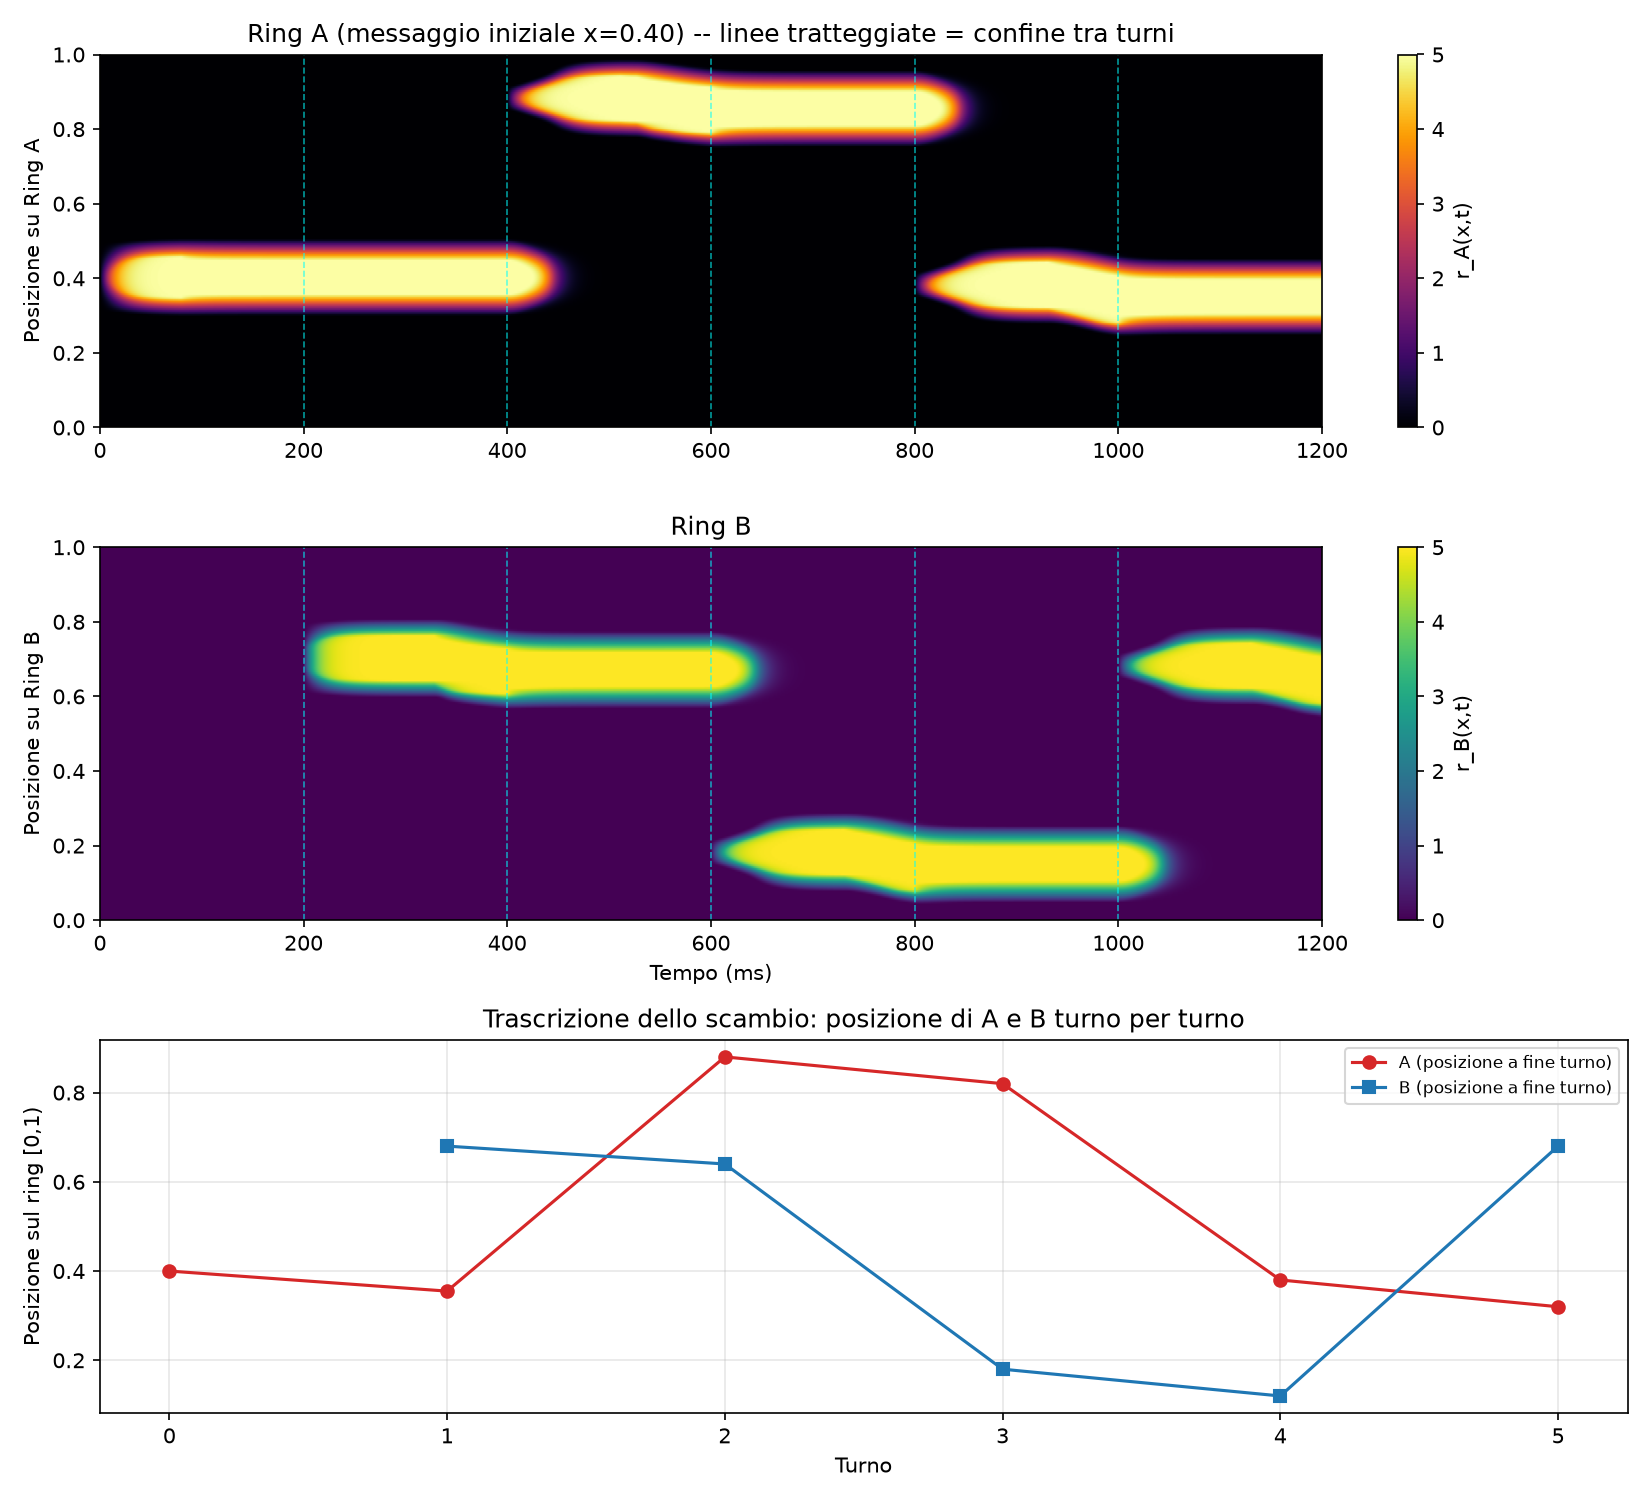
\includegraphics[width=5.8in,height=5.27273in]{media/media/image21.png}

\emph{Fig. 21 --- Turn-based exchange with fixed channels: raster of the two rings and turn-by-turn position transcript.}

\textit{\textbf{Source code: dialogo\_\allowbreak{}ring\_\allowbreak{}attractor.py}}

\lstinputlisting[language=Python]{scripts/dialogo_ring_attractor.py}
\subsubsection{5.5.2 Learned synapses with turn-grained Hebbian reinforcement}\label{learned-synapses-with-turn-grained-hebbian-reinforcement}

Here the two offset maps become two genuine N x N weight matrices (W\_\allowbreak{}AB and W\_\allowbreak{}BA), initialized to an innate bias DELIBERATELY too weak to light up a bump on its own in the listening network (activation threshold verified by bisection: between scale 0.0025, 0\% success, and 0.003, 100\% success -\/- the attractor is strongly bistable, with almost no middle ground). A Hebbian reinforcement at the end of each turn strengthens the pair (position of whoever just spoke, position of whoever just answered), every time the listener actually forms a bump. The chicken-and-egg problem -\/- without a working connection, a pair to reinforce is never observed -\/- is solved with an exploratory impulse to a random position during training only: random symmetry breaking, the same mechanism already verified in 5.2 (TEST 1b).

Result for the A-\textgreater B channel: B\textquotesingle s success rate goes from 0\% to 100\% in about 30-40 episodes (a sigmoidal curve, not an instantaneous jump), and the learned map converges to an offset of 0.195 -\/- different from the starting innate bias (0.3), a genuinely emergent result rather than an imposed one.

Result for the return channel B-\textgreater A: it does NOT consolidate in this script. A already has a persistent bump from turn 0 onward (it is an attractor), so B has to DISLODGE a bump already at full strength instead of lighting one up from zero -\/- a much harder task. The weight W\_\allowbreak{}BA does grow over time, but by pure statistical coincidence (A\textquotesingle s position stays almost always the same for reasons of its own, independent of B), not through any real causal influence: it remains behaviorally ineffective. A negative result verified with code, not hidden -\/- in the same methodological spirit stated in this document\textquotesingle s introduction.

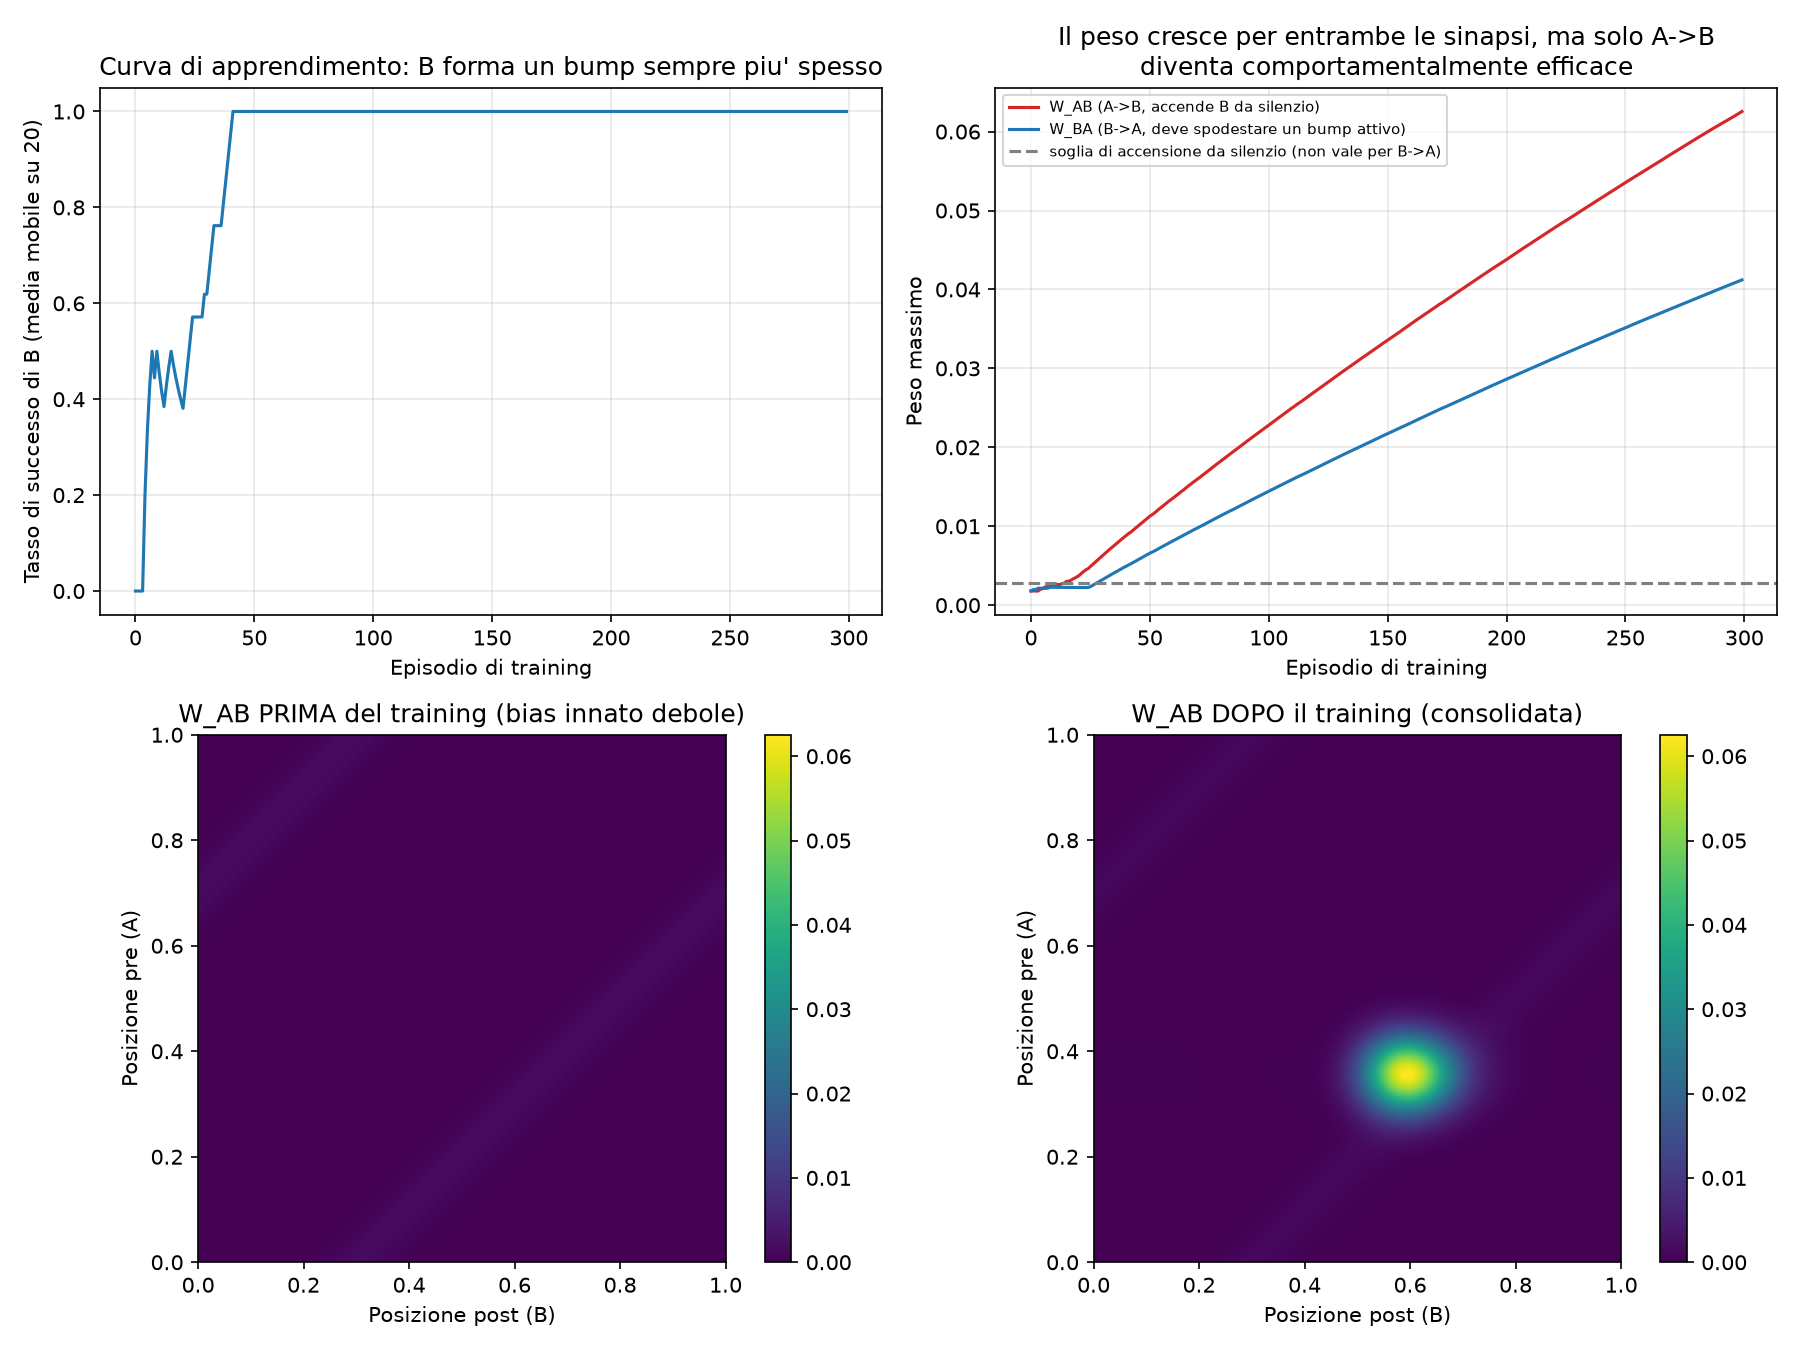
\includegraphics[width=5.8in,height=4.35in]{media/media/image22.png}

\emph{Fig. 22 --- Consolidation of the A-\textgreater B synapse: learning curve and weight map before/after.}

\textit{\textbf{Source code: dialogo\_\allowbreak{}stdp.py}}

\lstinputlisting[language=Python]{scripts/dialogo_stdp.py}
\subsubsection{5.5.3 Resolving the asymmetry: adaptation, silent turns, warm-up}\label{resolving-the-asymmetry-adaptation-silent-turns-warm-up}

To break the asymmetry of the previous step, a firing-threshold ADAPTATION is introduced -\/- the rate-model analogue of the recovery variable \textquotesingle u\textquotesingle{} in the Izhikevich model used throughout the rest of the project (Section 1.2): the longer a ring stays lit, the more a negative current grows until it eventually switches it off on its own. A dedicated test on an isolated ring shows that this model\textquotesingle s hard-clipped discharge makes the attractor strongly bistable (an abrupt collapse, not a soft decay); the adaptation parameter was chosen specifically so that a bump survives one full turn, weakens in the next, and collapses on its own one turn later. The problem thus returns to the one already solved (lighting up from silence), rather than dislodging a bump at full strength. A scheme with one SILENT turn between each listening turn proved necessary: without that pause, A would try to relight while adaptation was still at its peak and always failed.

Even with these two fixes, over 2000 episodes the B-\textgreater A synapse grew about 7 times slower than A-\textgreater B and never reached self-sufficiency. Diagnosis: in the early episodes B\textquotesingle s position has not yet stabilized (it depends on an A-\textgreater B channel not yet consolidated), so B-\textgreater A reinforcement initially targets a moving target and dilutes instead of concentrating. Fixed with a WARM-UP phase (A-\textgreater B only for the first 400 episodes) and a higher learning rate for B-\textgreater A.

Final result, with a sufficient training budget (\textasciitilde2500 episodes): ALL four exchanges tested reach 100\% reliability in clean evaluation (frozen weights, no exploratory noise) -\/- B responds at turn 1 and again at turn 5, A responds at turn 3 and again at turn 7. Turn 5 and turn 7 are SECOND-ORDER associations (the network must respond to the position the other party took AFTER it has already answered once, not to the original message): they consolidate only after the first response is already stable, so they require more episodes and appear in the final weight map as secondary reinforcements, weaker than the main peak. The starting asymmetry (B-\textgreater A not learning at all) is resolved in this run, not merely reduced.

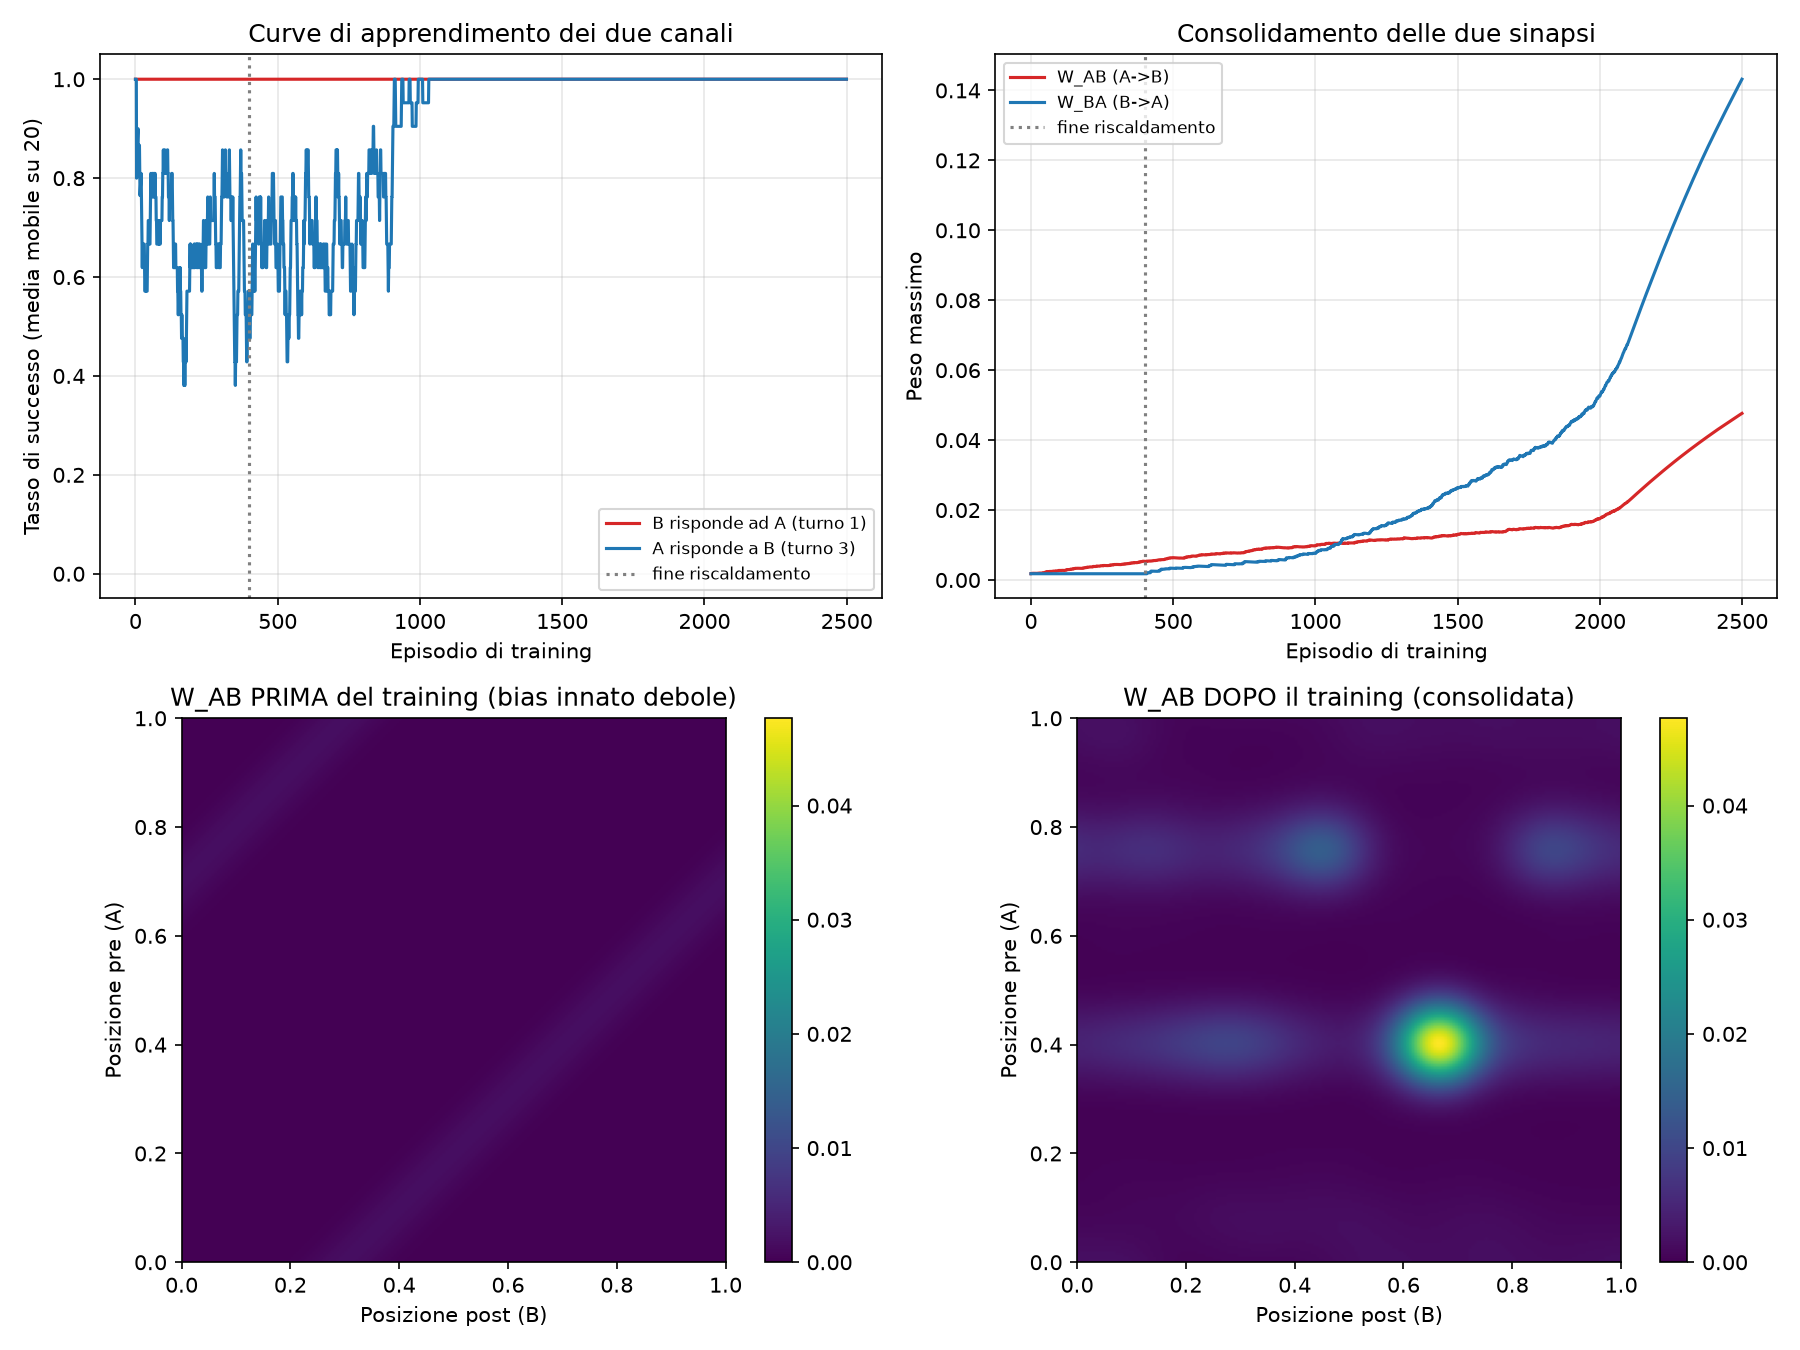
\includegraphics[width=5.8in,height=4.35in]{media/media/image23.png}

\emph{Fig. 23 --- Learning curves for both channels, consolidation of the two synapses, W\_\allowbreak{}AB map before/after.}

\textit{\textbf{Source code: dialogo\_\allowbreak{}stdp\_\allowbreak{}adattamento.py}}

\lstinputlisting[language=Python]{scripts/dialogo_stdp_adattamento.py}
\subsubsection{5.5.4 More messages on the same synapse: an interference test}\label{more-messages-on-the-same-synapse-an-interference-test}

Last question, the real generalization test in the same spirit as Section 5.4 (which extends a single context to several contexts): can the SAME pair of synapses W\_\allowbreak{}AB/W\_\allowbreak{}BA, shared (not a separate matrix per message), learn to distinguish SEVERAL different messages without interfering with each other? Two well-separated messages on the ring (x=0.15 and x=0.65) are alternated during training.

Result after 3000 episodes with the message chosen randomly on each episode: no interference on the return channel (B-\textgreater A at 100\% for both messages, at both turn 3 and turn 7), but the A-\textgreater B channel fully consolidates for only one of the two messages (x=0.65: 100\%; x=0.15: 0\%) -\/- one possible explanation, at that point, was simple unequal exposure during the random draw.

To verify this, the experiment was rerun with the messages alternated in ROUND-ROBIN order instead of randomly drawn (9000 episodes, identical exposure guaranteed by construction) -\/- and the result disproved that explanation. The A-\textgreater B channel did not consolidate for both: it simply flipped which of the two messages wins (now x=0.15 reaches 100\% on all four exchanges, including turn 5, which had never consolidated before; x=0.65 collapses to 0\% on both turn 1 and turn 5). With equal exposure guaranteed, the winner changes but the phenomenon stays identical: it is real competitive interference on the A-\textgreater B channel -\/- verified across two independent runs, not an artifact of unequal exposure -\/- while the B-\textgreater A channel remains completely free of interference in both runs. The final weight map shows a single clean peak (for the winning message) instead of the two separate regions one would expect from competition-free learning: an honest but not yet fully explained result, left as an open question (similar in spirit to the ring attractor\textquotesingle s position bias, Section 9) rather than forced into a more convenient conclusion than the one observed.

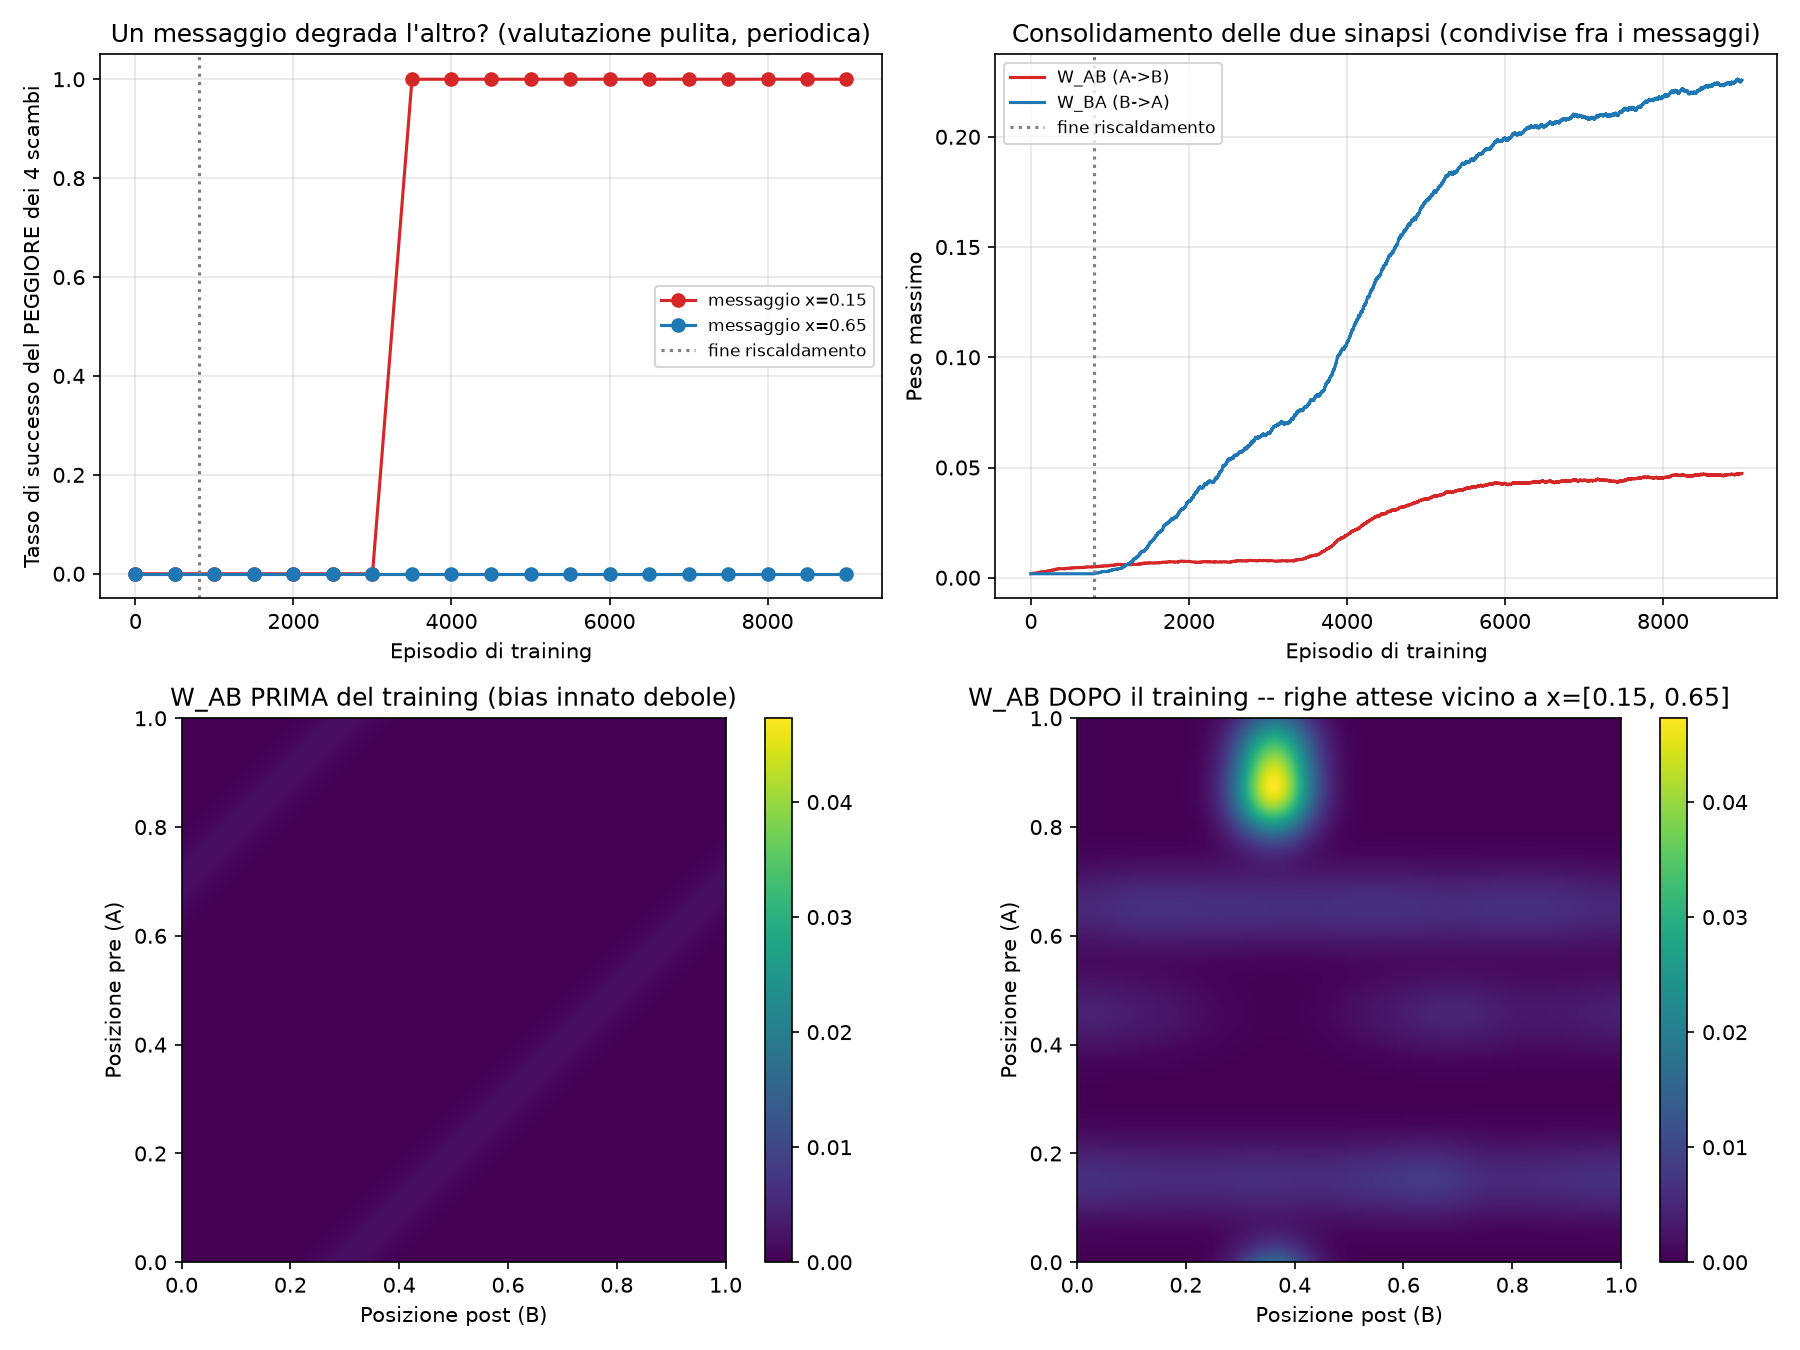
\includegraphics[width=5.8in,height=4.35in]{media/media/image25.png}

\emph{Fig. 24 --- Interference test between two messages (round-robin, 9000 episodes): B-\textgreater A clean at 100\% for both; A-\textgreater B shows a competitive win by a single message, with one clean peak in the final weight map.}

\textit{\textbf{Source code: dialogo\_\allowbreak{}multi\_\allowbreak{}messaggio.py}}

\lstinputlisting[language=Python]{scripts/dialogo_multi_messaggio.py}
\subsubsection{5.5.5 An attempted correction: homeostatic normalization (partial result)}\label{an-attempted-correction-homeostatic-normalization-partial-result}

The interference observed in 5.5.4 suggests two possible explanations: either the synapses grow without bound and one message ends up monopolizing the shared matrix, or the problem lies in B\textquotesingle s own attractor dynamics (once a strong bump has settled in one zone, that zone becomes a basin of attraction that is also easier to reach for different inputs). The first explanation can be tested directly: a HOMEOSTATIC NORMALIZATION is added to W\_\allowbreak{}AB -\/- the total of incoming weights onto each of B\textquotesingle s neurons (column sum) cannot exceed a fixed cap, calibrated a bit above the value reached in a single-message reference run (Section 5.5.3). It is a biologically motivated mechanism: real neurons homeostatically regulate the total of their incoming synapses. A single-message regression test confirms that normalization does not interfere with learning when there is no competition (the column total stays well below the cap throughout training).

Result with two messages (same configuration as Section 5.5.4: 9000 episodes, round-robin): normalization does NOT reverse the outcome -\/- x=0.15 still wins and reaches 100\% on all four exchanges, while x=0.65 fails on B\textquotesingle s primary response (turn 1). But something new appears: for the first time a genuine TRANSIENT INSTABILITY is observed (around episode 7000, x=0.65 briefly reaches 100\% on all four exchanges before falling back to 0\%) -\/- direct evidence that the cap is creating real competition, not being ignored. And the losing message still gets a partial improvement: its second-order response (turn 5) reaches 100\% in the final evaluation, something that never happened without normalization. The W\_\allowbreak{}AB peak is lower than in the previous run (0.036 vs. 0.047), a sign that the cap is genuinely limiting growth.

Interpretation: normalization changes the competitive dynamics but not the final outcome. This favors the second explanation, not the first -\/- the bottleneck appears to be B\textquotesingle s attractor dynamics (which basin becomes dominant), not simply the available synaptic capacity. Limiting weights makes the competition visible without resolving it. A more direct test of this hypothesis -\/- for instance separating B\textquotesingle s global inhibition component by zone rather than over the whole population -\/- remains future work, not addressed here: an honest but not yet fully explained result, left as an open question rather than forced into a solution.

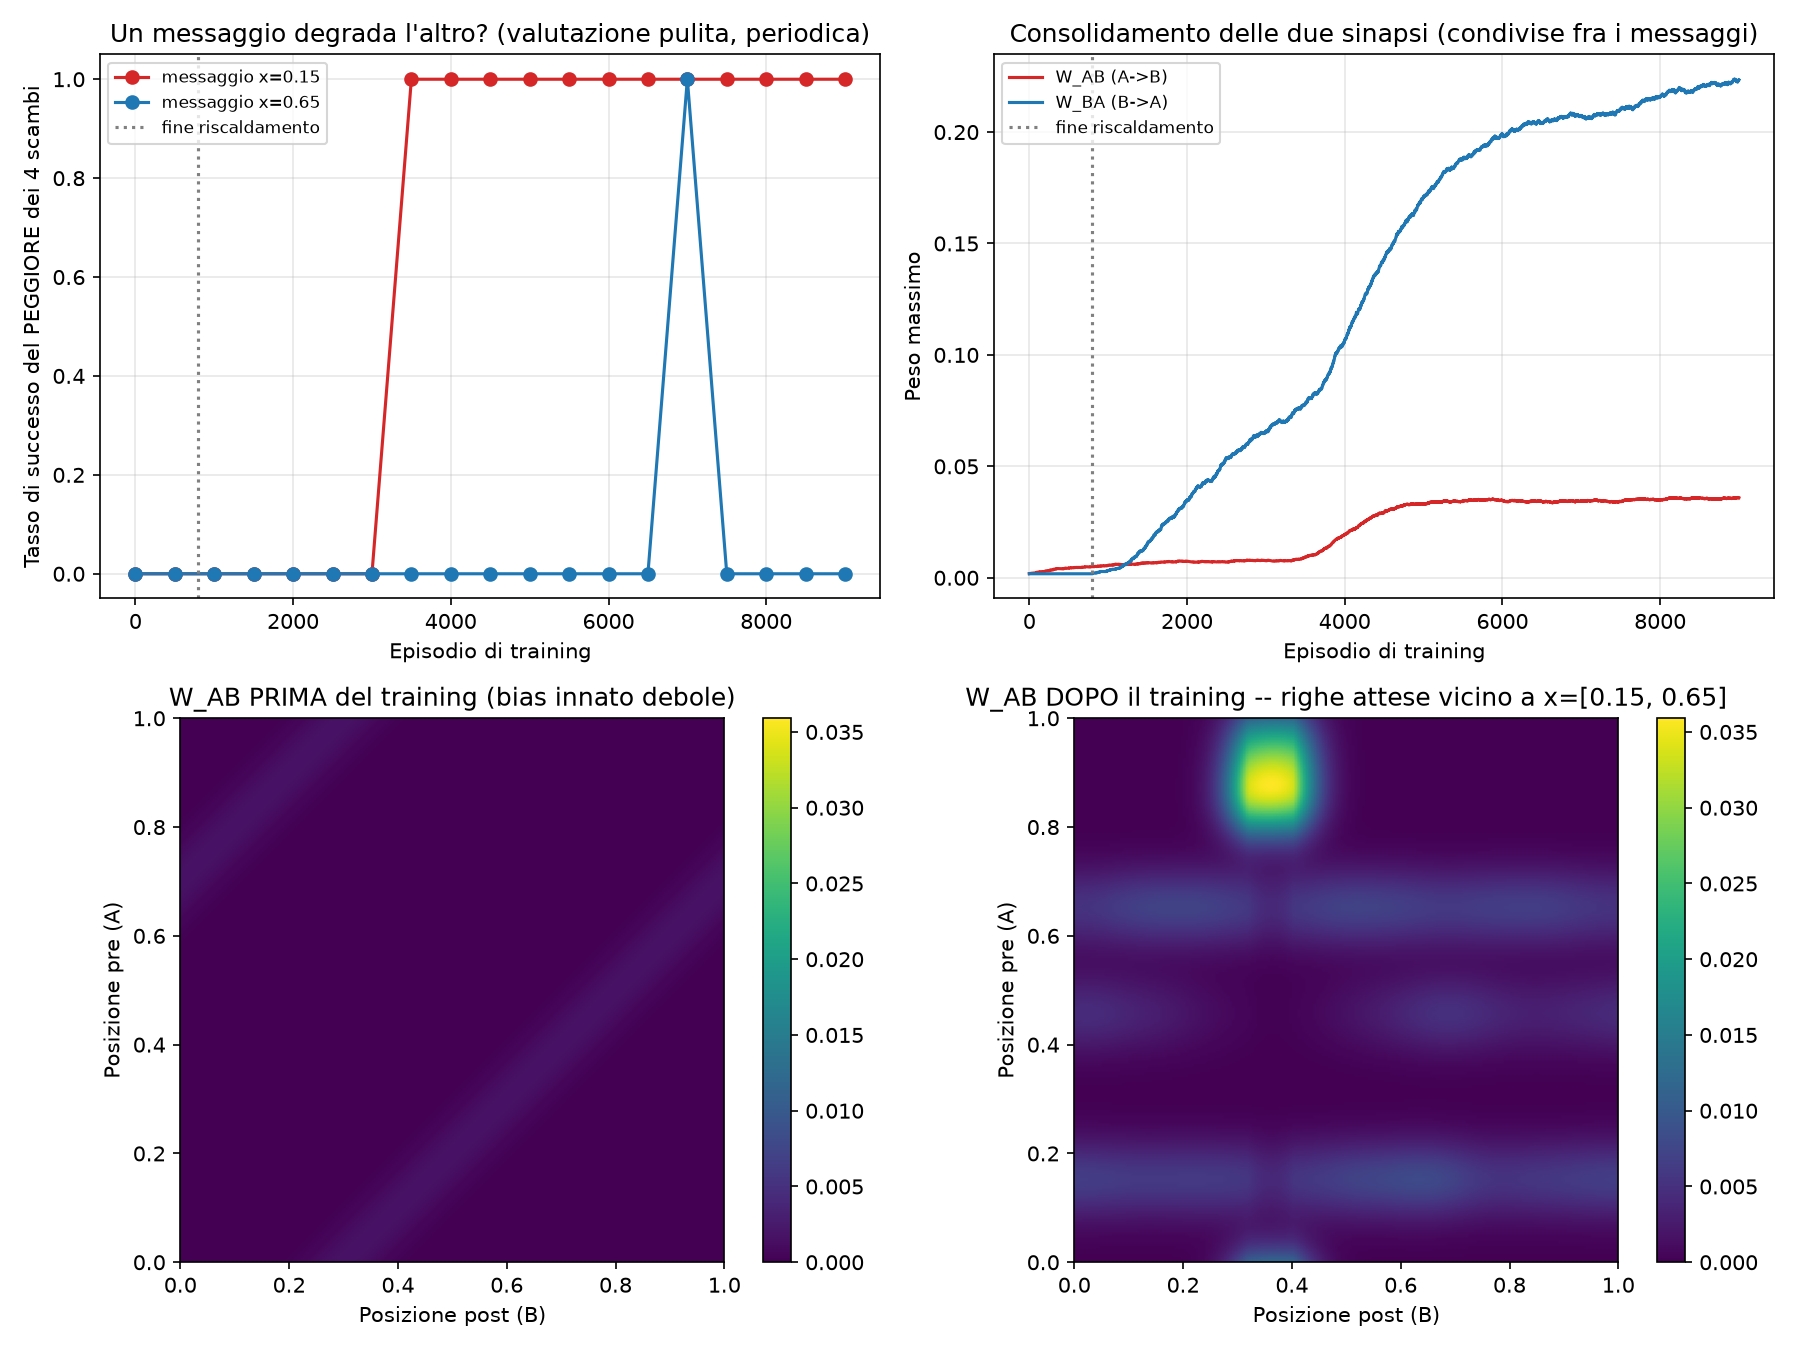
\includegraphics[width=5.8in,height=4.35in]{media/media/image26.png}

\emph{Fig. 25 --- Same interference test with homeostatic normalization on W\_\allowbreak{}AB: the outcome does not change, but a transient instability appears (episode \textasciitilde7000) that was absent without normalization.}

\textit{\textbf{Source code: dialogo\_\allowbreak{}multi\_\allowbreak{}normalizzato.py}}

\lstinputlisting[language=Python]{scripts/dialogo_multi_normalizzato.py}
\subsubsection{5.5.6 Successful correction: repulsive exploration}\label{successful-correction-repulsive-exploration}

Normalization (5.5.5) had shown that limiting synaptic capacity is not enough: it makes competition visible but does not resolve it. A different hypothesis: perhaps the two messages are not really competing for a shared resource, but the random SEARCH (the exploratory impulse to a uniformly random position) rediscovers by pure chance the same "easy" zone of the ring for both -\/- consistent with the position bias already documented for the ring attractor (Section 9). The correction proposed here does not touch synaptic capacity but the SEARCH itself: the exploratory impulse is now drawn with a probability inversely proportional to how much a zone is already occupied by OTHER messages (excluding one\textquotesingle s own row, so as not to repel a message from the zone it is still trying to consolidate -\/- an error explicitly avoided after a dedicated regression test). A message still without a response is thus pushed toward free territory rather than toward territory already claimed by another.

Result (same configuration as Sections 5.5.4-5.5.5: 9000 episodes, round-robin): the final weight map shows, for the first time, TWO distinct and well-separated rows, one for each message (x=0.15 and x=0.65), each with its own response zone in B, with no visible overlap. In clean evaluation, SEVEN exchanges out of eight reach 100\% (both messages at 100\% on B turn 1, A turn 3, A turn 7; x=0.65 also at 100\% on B turn 5) -\/- only x=0.15\textquotesingle s turn 5 stays at 0\%, the deepest (third-order) association and the slowest to consolidate already in earlier sections. The periodic learning curve also shows that even x=0.65 unlocked that response only at the VERY LAST checkpoint of training (episode 8999 of 9000): x=0.15 appears to be on the same trajectory, just slightly behind by pure chance, not blocked by structural interference.

NOTE (corrected after direct verification, Section 5.5.7): the hypothesis that the problem was a systematic position bias of the ring attractor -\/- a few "easy" points on the ring rediscovered by chance by different messages -\/- was later tested directly by training several messages completely independently (no shared synapse) and checking whether the response positions clustered. They did not (Section 5.5.7): they come out scattered in a way compatible with a uniform distribution. The position-bias hypothesis must therefore be ABANDONED as the explanation for this phenomenon. The correction (repulsive exploration) remains effective nonetheless, for a simpler and correct reason: when messages share the SAME matrix during concurrent training, repulsion based on the CURRENT occupancy of that matrix (regardless of the cause of that occupancy) still prevents collisions, without any need for an independent upstream position bias to exist.

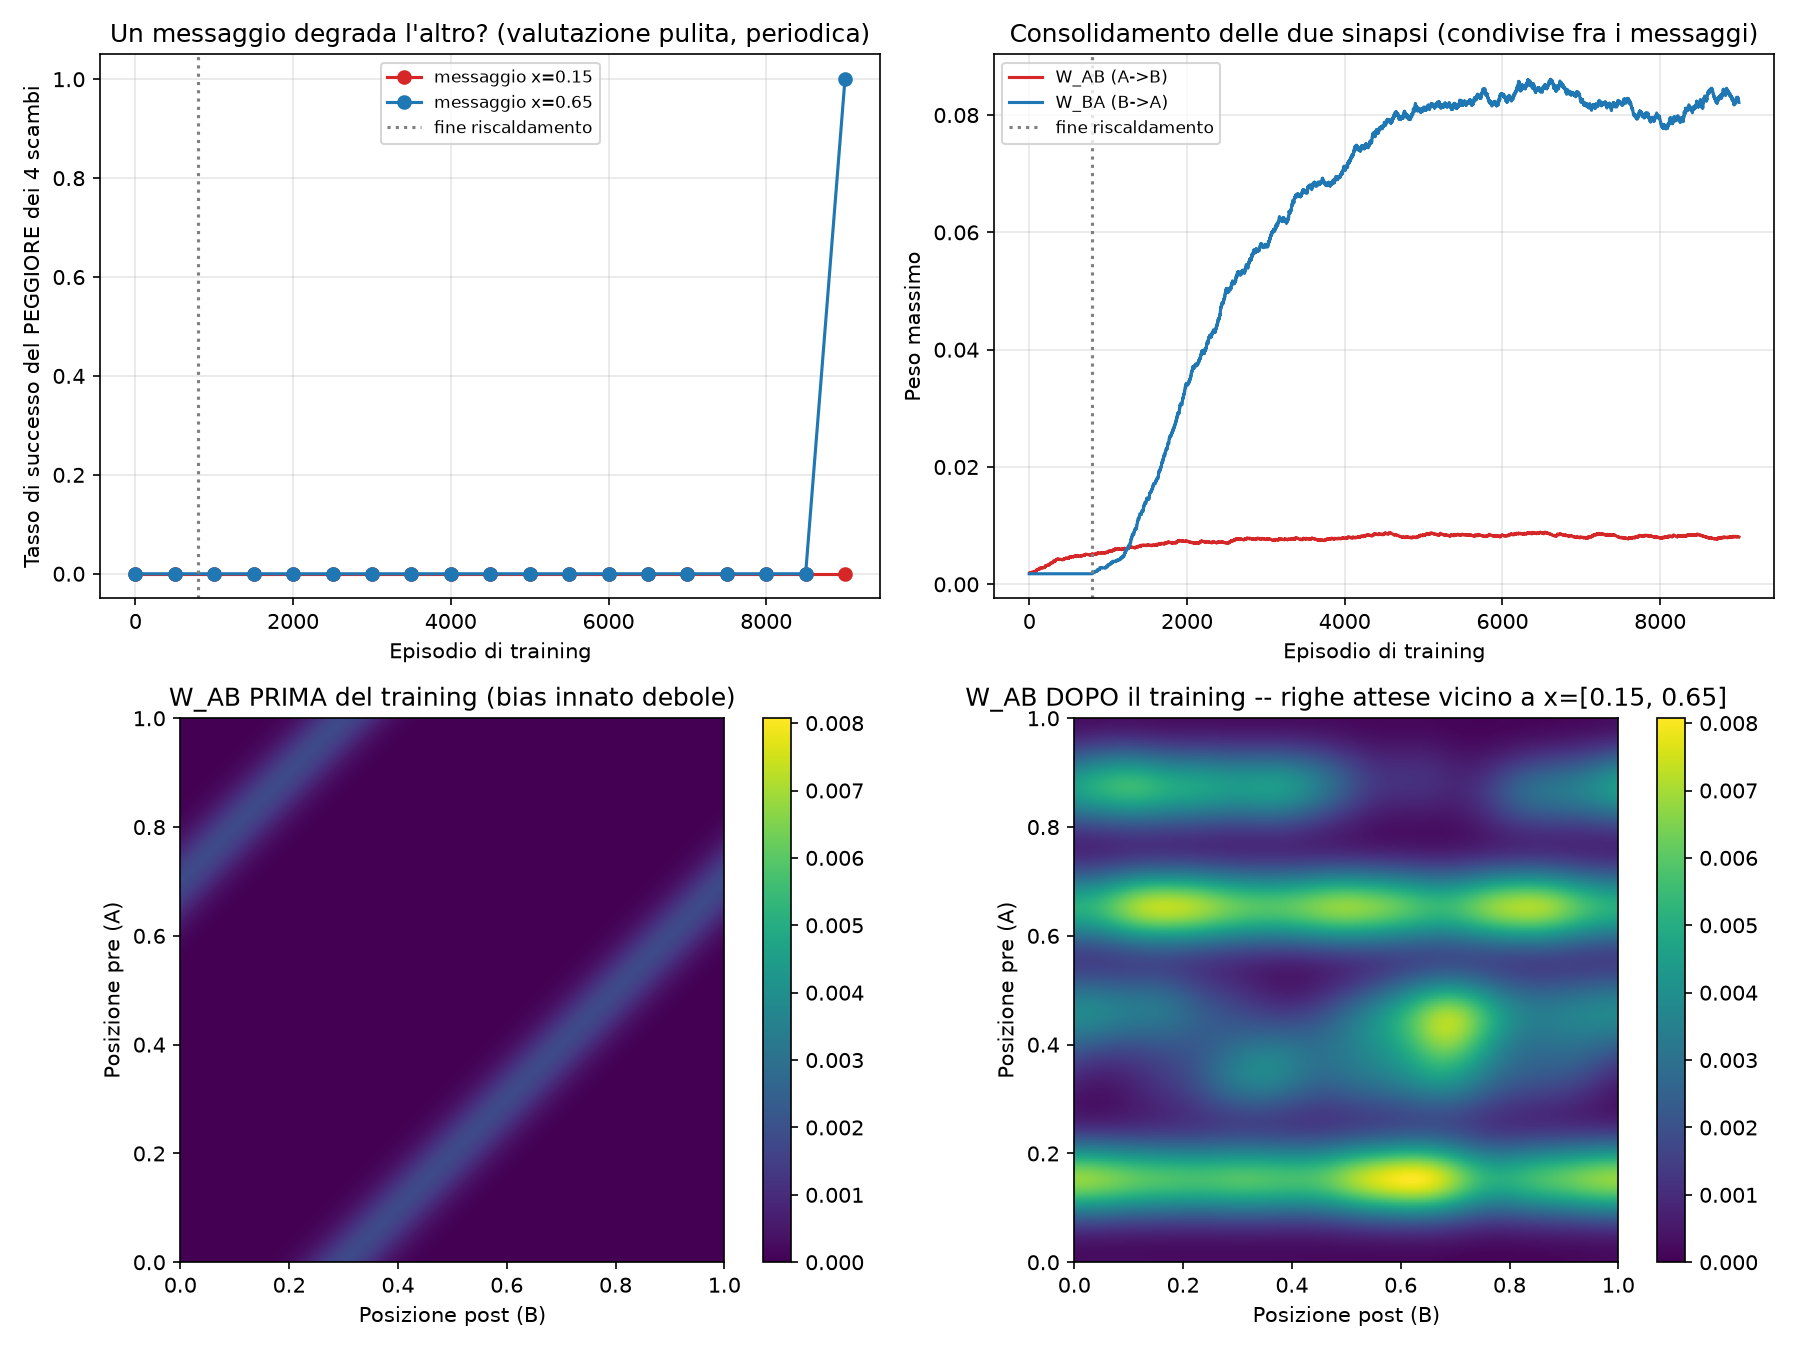
\includegraphics[width=5.8in,height=4.35in]{media/media/image27.png}

\emph{Fig. 26 --- With repulsive exploration: two distinct, separated rows in the weight map, 7 of 8 exchanges at 100\%.}

\textit{\textbf{Source code: dialogo\_\allowbreak{}multi\_\allowbreak{}repulsione.py}}

\lstinputlisting[language=Python]{scripts/dialogo_multi_repulsione.py}
\subsubsection{5.5.7 Direct test of the position-bias hypothesis (disproved)}\label{direct-test-of-the-position-bias-hypothesis-disproved}

Section 5.5.6 had explained the success of repulsion with the hypothesis that memoryless random search would, by pure chance, rediscover the same "easy" zone of the ring for different messages -\/- linking it to the position bias already documented for the ring attractor (Section 9). Such a hypothesis can be tested directly, not merely argued: many different messages are trained COMPLETELY INDEPENDENTLY (a fresh network for each, no shared weights, no repulsion -\/- the only thing in common is the ring attractor\textquotesingle s physics) and the final response positions are checked for clustering.

Result with 6 independent messages, evenly spaced around the ring (0.05, 0.20, 0.35, 0.50, 0.65, 0.80): the learned target positions (0.360, 0.185, 0.345, 0.680, 0.965, 0.130) come out SCATTERED, not clustered. The mean circular distance between pairs of positions (0.260) coincides almost exactly with what would be expected for uniformly and independently distributed points on the ring (\textasciitilde0.26). No evidence of clustering in this sample.

The position-bias hypothesis as the cause of the interference must therefore be ABANDONED -\/- and the corresponding paragraph in 5.5.6 has been corrected accordingly. This does not invalidate the correction (repulsive exploration remains effective, empirically verified), but it changes the correct explanation for it: repulsion works because it counters the REAL collision that arises when two search processes share the SAME matrix during CONCURRENT training -\/- not because an independent upstream position bias exists. It is a useful methodological reminder, in the same spirit stated in this document\textquotesingle s introduction: a correction can work for a different reason than the one under which it was proposed, and the only way to know is to test the explanation itself, not just its effect.

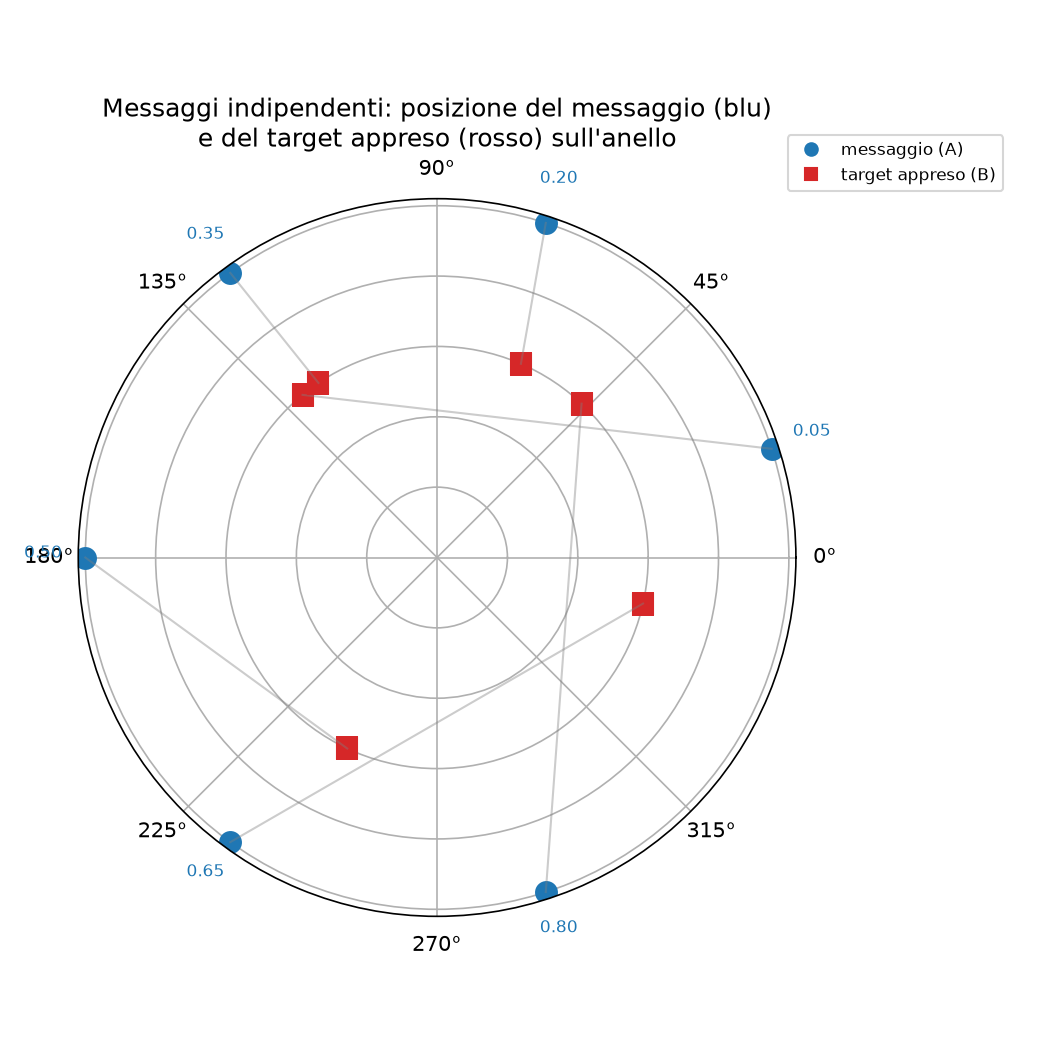
\includegraphics[width=5.8in,height=5.8in]{media/media/image28.png}

\emph{Fig. 27 --- Six independently trained messages: the target positions (red) do not cluster around the message (blue) nor among themselves.}

\textit{\textbf{Source code: diagnosi\_\allowbreak{}bias\_\allowbreak{}posizione.py}}

\lstinputlisting[language=Python]{scripts/diagnosi_bias_posizione.py}
\subsubsection{5.5.8 Scaling to 3 messages: better separation, worse consolidation}\label{scaling-to-3-messages-better-separation-worse-consolidation}

A direct scaling question: does the correction that worked for 2 messages (5.5.6) still hold with 3? Same mechanism, no change to the algorithm, only the training budget scaled proportionally (WARMUP and N\_\allowbreak{}EPISODES tripled to give each message the same number of effective episodes as the 2-message version).

First attempt (REPULSIONE\_\allowbreak{}ESPLORAZIONE=5, the same value as the 2-message version, 13500 episodes): a partial but consistent result -\/- all three messages show the SAME pattern (they respond on A turn 3, B turn 5, A turn 7, but fail on B turn 1), 9 exchanges out of 12 succeed. The weight map, however, reveals the reason: a single second-order association dominates at the expense of the three primary rows, which stay weak -\/- with 3 messages (which also generate their own derived associations), the demand for distinct "slots" on the ring exceeds what a repulsion tuned for 2 messages can separate.

Second attempt, to reinforce separation: REPULSIONE\_\allowbreak{}ESPLORAZIONE raised to 20 (4x) and the budget increased further (18000 episodes). Result: the final weight map NOW shows three distinct rows correctly positioned near x=0.1, 0.4, 0.7 -\/- separation improved, exactly as expected. But the success rate got WORSE (6 exchanges out of 12 instead of 9), and the W\_\allowbreak{}AB peak collapsed to 0.0067 (against 0.0411 in the first attempt) -\/- channel B almost never lights up even in clean evaluation. Repulsion that is too strong fails to discriminate between "zone occupied by ANOTHER message" (to avoid) and "small natural variation around one\textquotesingle s own position" (not to be penalized): it ends up repelling legitimate reinforcement too, not just collisions, preventing the rows from consolidating enough to cross the threshold for autonomous activation.

Conclusion: separation of associations and strength of consolidation are two objectives in TENSION, not aligned as one might expect -\/- reinforcing repulsion gets one at the expense of the other. The right value is probably somewhere between 5 and 20, not yet found in this work: an honest but incomplete result, left as an open question rather than forced into a more convenient conclusion than the one observed.

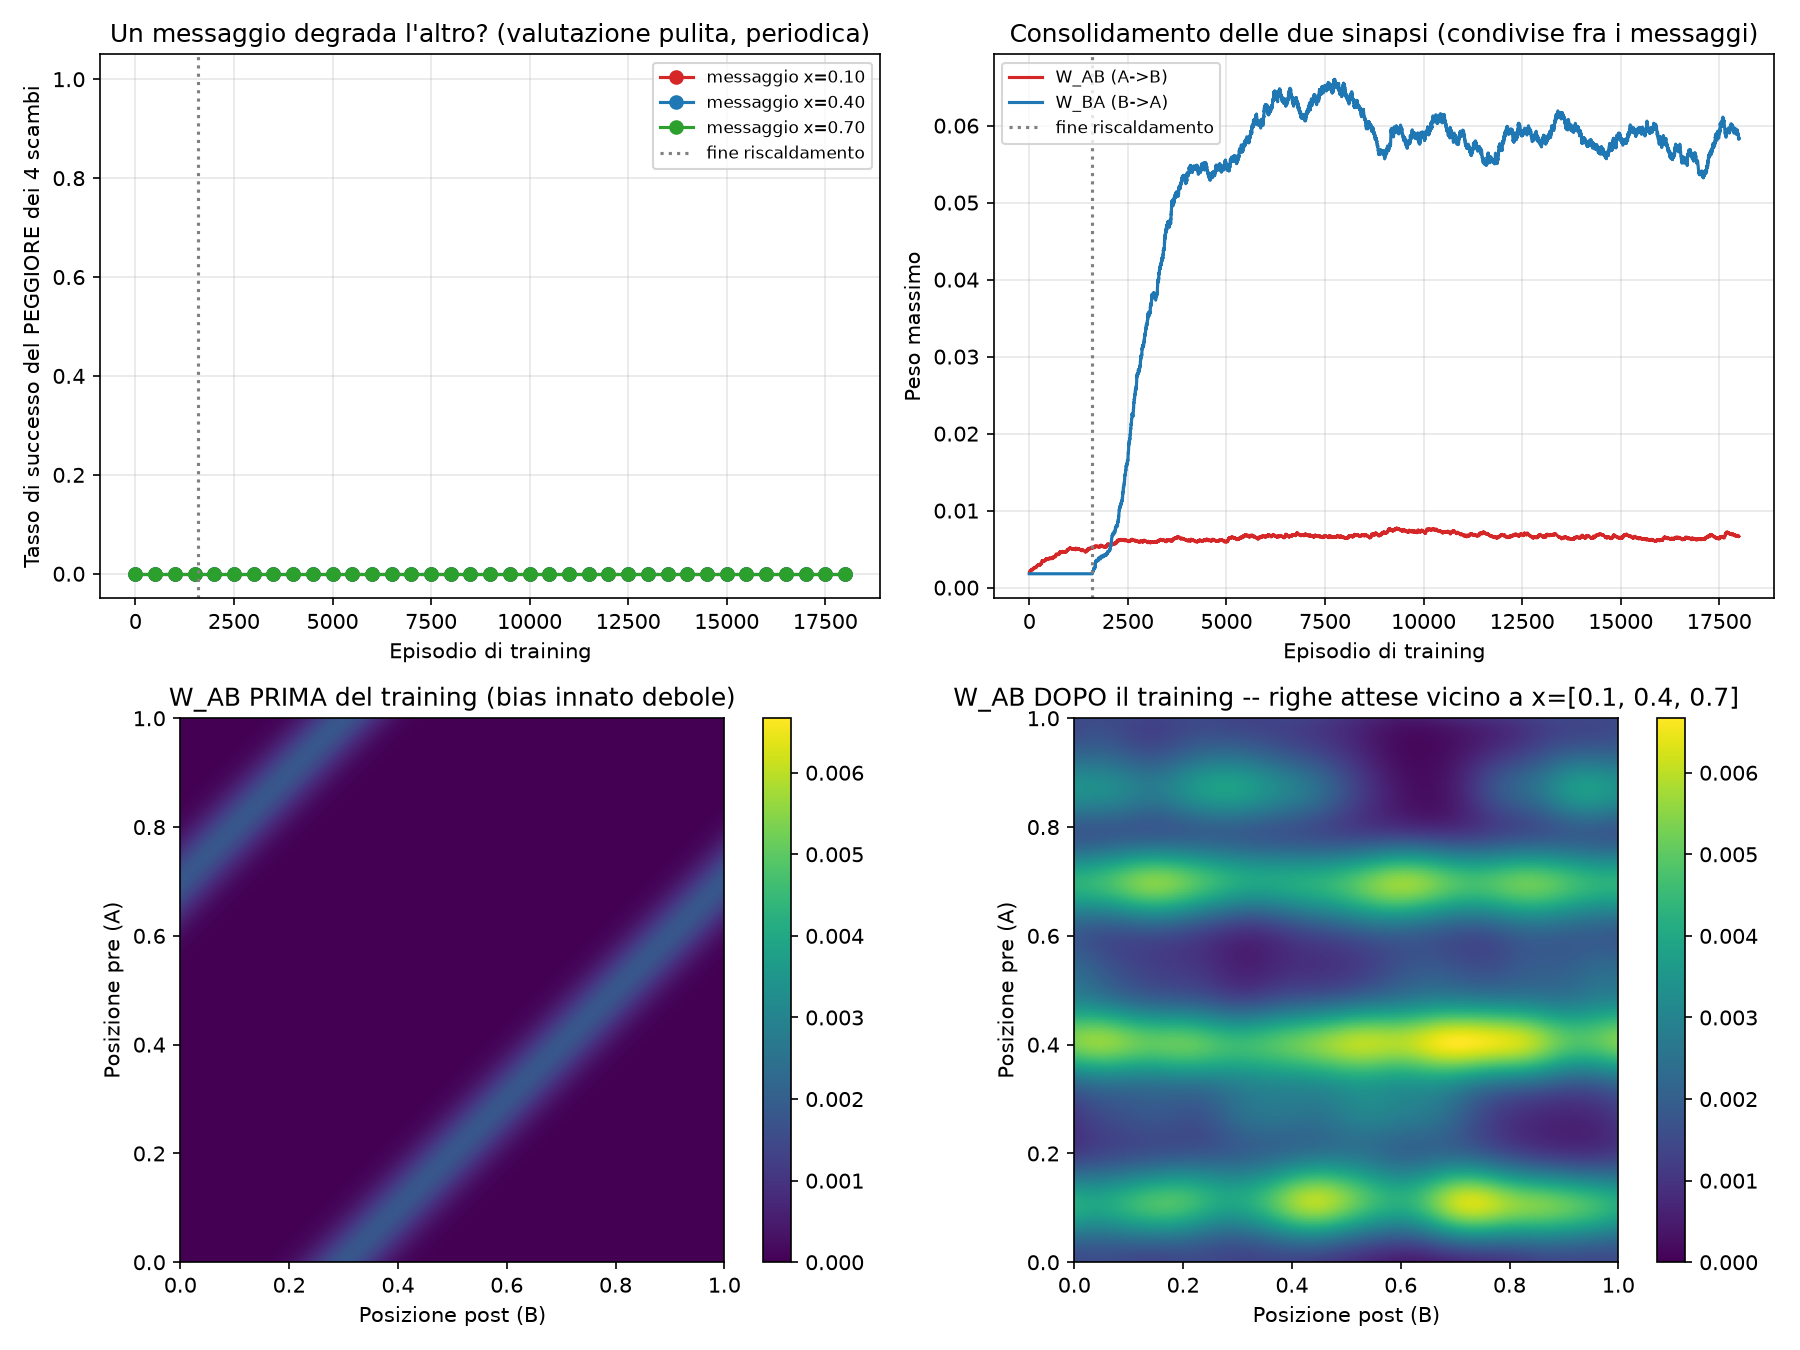
\includegraphics[width=5.8in,height=4.35in]{media/media/image29.png}

\emph{Fig. 28 --- Scaling to 3 messages with reinforced repulsion: better-separated rows, but weaker consolidation (6/12 instead of 9/12).}

\textit{\textbf{Source code: dialogo\_\allowbreak{}multi\_\allowbreak{}repulsione\_\allowbreak{}3msg.py}}

\lstinputlisting[language=Python]{scripts/dialogo_multi_repulsione_3msg.py}
\subsubsection{5.5.9 Decisive correction: repulsion only for discovery, local exploration for consolidation}\label{decisive-correction-repulsion-only-for-discovery-local-exploration-for-consolidation}

Three previous attempts (5.5.6 with weak repulsion, 5.5.8 with strong fixed repulsion and with annealing) had shown an unresolved tension: repulsion strong enough to separate the three primary rows well left consolidation weak (W\_\allowbreak{}AB peak \textasciitilde0.006-0.007), while weak repulsion allowed strong consolidation but with the rows colliding (a single dominant derived association). Revised diagnosis: the problem was not the STRENGTH of repulsion but the fact that it stayed active for the ENTIRE training run. Even after a message had already found a zone, every new exploratory attempt was still redrawn from the GLOBAL repulsive distribution -\/- which shifts slightly every time OTHER messages train -\/- preventing reinforcement from concentrating at a stable point even once separation had already been achieved.

Correction: two phases per message, not a single fixed strategy for the whole training run. As long as a message has not yet found a first valid response, repulsive exploration (as before, used to separate the initial discoveries). Once a first response is found, the message switches to LOCAL exploration -\/- a small jitter around the position already discovered -\/- instead of continuing to redraw from the global distribution: consolidation no longer depends on what happens elsewhere in the matrix while other messages train.

Result (same configuration as previous trials: 13500 episodes, round-robin, 3 messages): 10 exchanges out of 12 succeed -\/- the best so far, against 9/12 in the first attempt with weak repulsion. Two of the three messages (x=0.10 and x=0.40) reach 100\% on ALL four exchanges, with a notable detail: their learned offsets (0.300 and 0.295) coincide almost exactly with the innate bias (0.3) -\/- a much cleaner convergence than any previous run, where the final offset tended to drift quite far from the starting bias. The third message (x=0.70) reaches 2/4 (B turn 1 and A turn 3 succeed; B turn 5 and A turn 7 do not). The training curves also show a qualitatively different and healthier dynamic compared to every previous attempt: x=0.10 and x=0.40 reach 100\% (around episode \textasciitilde1500 and \textasciitilde2000) and stay there stably until the end, WITHOUT the continuous oscillation observed in every previous attempt. The final weight map shows three sharp, compact, well-separated spots -\/- no longer blurred bands or a single dominant peak.

The residual (x=0.70 on the higher-order associations) is most likely just a matter of luck in discovery order (in the round-robin, x=0.70 is always the last of the three in every cycle) rather than a new structural limit -\/- consistent with what has already been observed elsewhere in this document (higher-order associations systematically require more episodes than the first ones, Section 5.5.3). Separating the discovery phase from the consolidation phase thus resolves the central tension diagnosed in 5.5.8, without the trade-off observed in the attempts using a single fixed strategy for the whole training run.

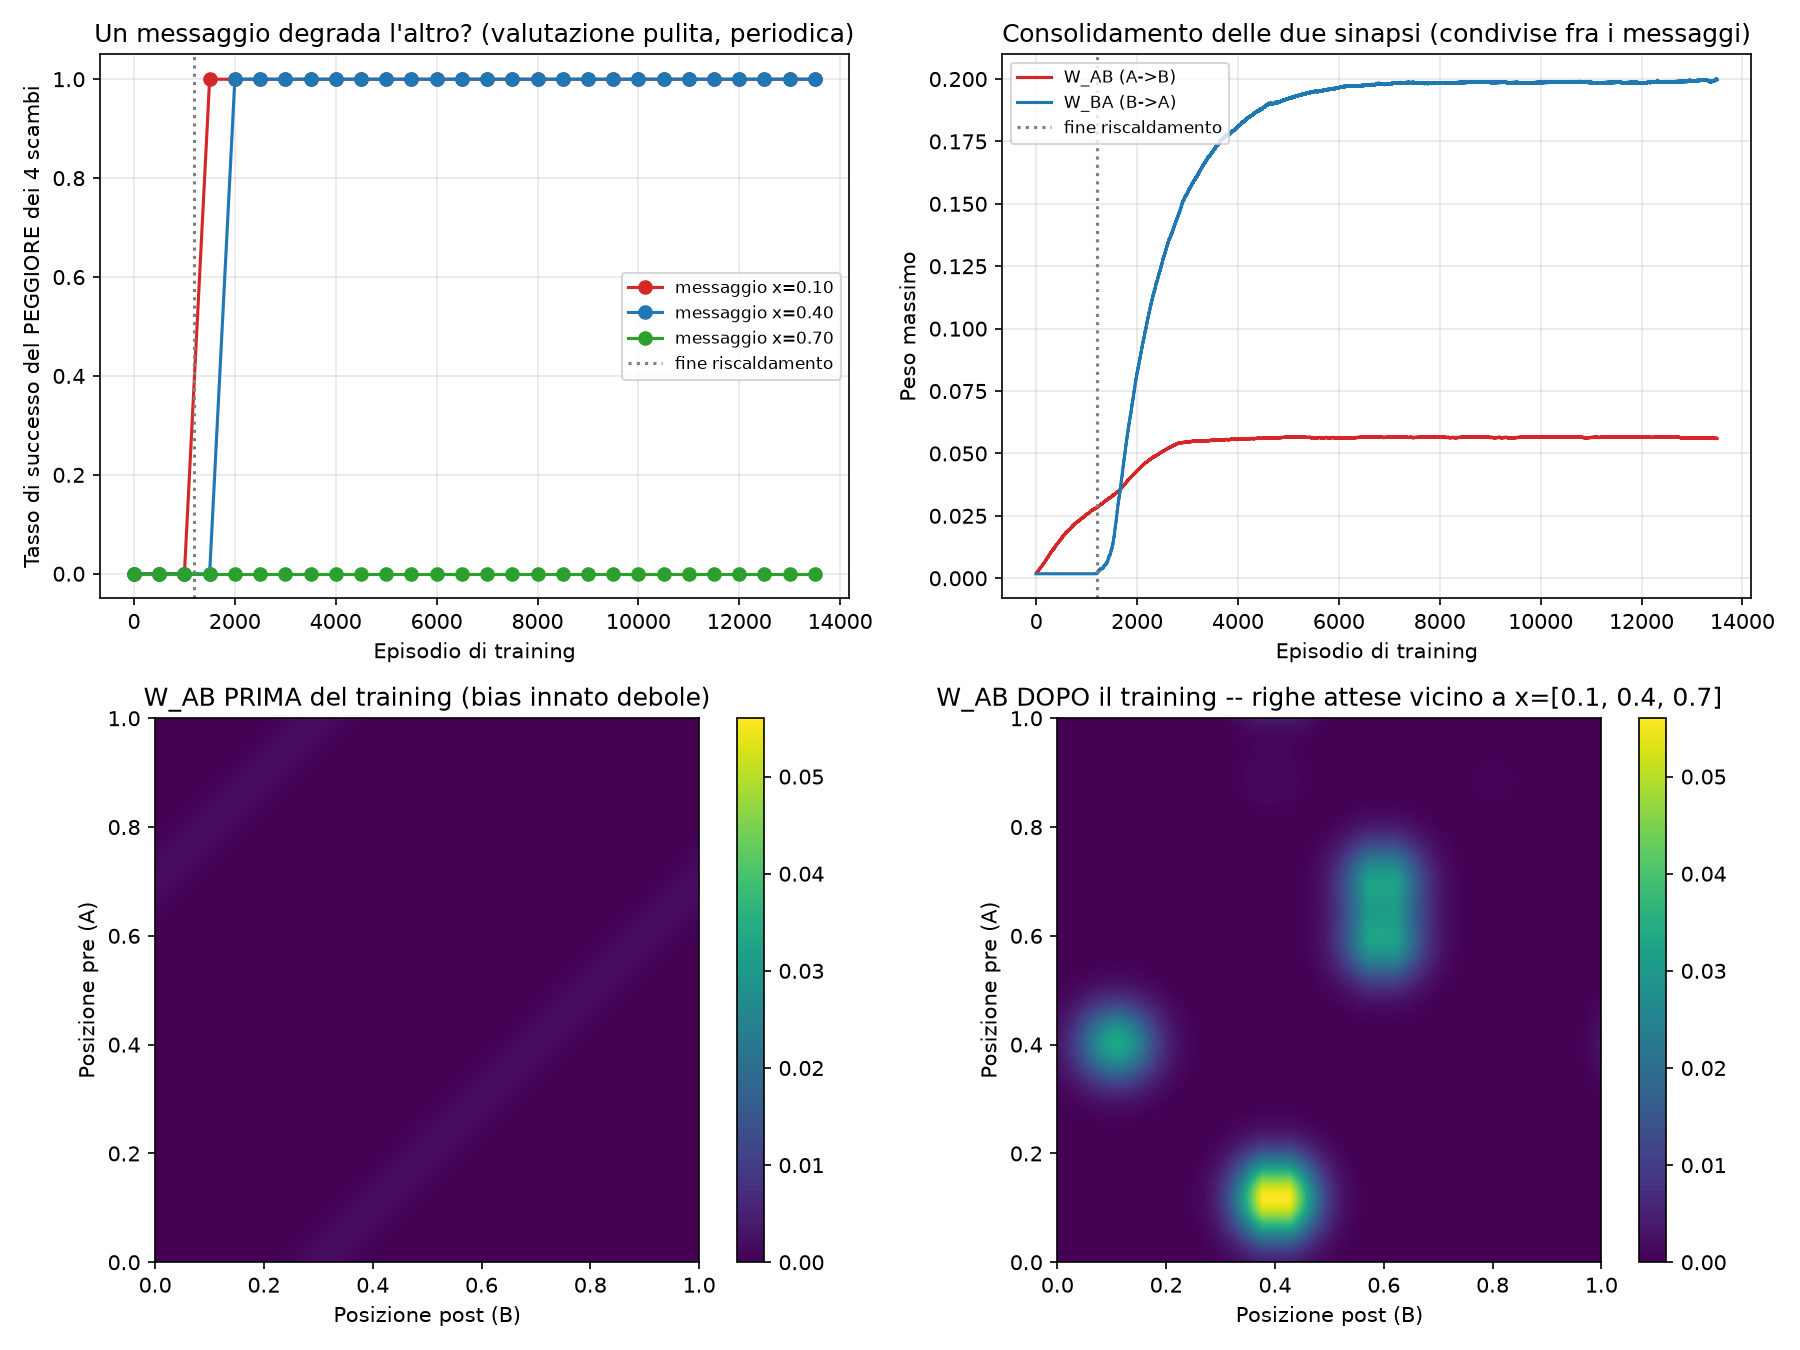
\includegraphics[width=5.8in,height=4.35in]{media/media/image30.png}

\emph{Fig. 29 --- Repulsive discovery + local consolidation: 10/12 exchanges, two of three messages perfect, weight map with three sharp, separated spots.}

\textit{\textbf{Source code: dialogo\_\allowbreak{}multi\_\allowbreak{}scoperta\_\allowbreak{}locale.py}}

\lstinputlisting[language=Python]{scripts/dialogo_multi_scoperta_locale.py}
\subsubsection{5.5.10 Monte Carlo verification: the result is robust, but the hypothesis about the residual was wrong}\label{monte-carlo-verification-the-result-is-robust-but-the-hypothesis-about-the-residual-was-wrong}

Section 5.5.9 had obtained 10 exchanges out of 12 with a single random seed, and had attributed the residual (the third message, last in the round-robin, which did not reach the higher-order associations) to bad luck in discovery order. A single run is not enough to confirm this -\/- the same statistical principle already applied in the project (PSTH over 25 independent trials, Section 2.11) requires repeating the experiment with different SEEDS before drawing conclusions about why a result comes out a certain way. Eight independent replicates (exact same configuration, no change to the algorithm, only the rng\_\allowbreak{}train seed) were run in parallel.

Aggregate result: 88 successes out of 96 total checks (8 seeds x 3 messages x 4 exchanges) = 91.7\% -\/- higher than the single original run (83\%), confirming that the discover-then-consolidate-locally mechanism is robust, not an isolated stroke of luck. Turn 1 (B responds) and turn 3 (A responds) turned out to be PERFECTLY reliable: 100\% for all three messages, in all 8 seeds without exception.

{\def\LTcaptype{none} % do not increment counter
\begin{longtable}[]{@{}
  >{\raggedright\arraybackslash}p{(\linewidth - 8\tabcolsep) * \real{0.2000}}
  >{\raggedright\arraybackslash}p{(\linewidth - 8\tabcolsep) * \real{0.2000}}
  >{\raggedright\arraybackslash}p{(\linewidth - 8\tabcolsep) * \real{0.2000}}
  >{\raggedright\arraybackslash}p{(\linewidth - 8\tabcolsep) * \real{0.2000}}
  >{\raggedright\arraybackslash}p{(\linewidth - 8\tabcolsep) * \real{0.2000}}@{}}
\toprule\noalign{}
\begin{minipage}[b]{\linewidth}\raggedright
Message
\end{minipage} & \begin{minipage}[b]{\linewidth}\raggedright
B (turn 1)
\end{minipage} & \begin{minipage}[b]{\linewidth}\raggedright
A (turn 3)
\end{minipage} & \begin{minipage}[b]{\linewidth}\raggedright
B (turn 5)
\end{minipage} & \begin{minipage}[b]{\linewidth}\raggedright
A (turn 7)
\end{minipage} \\
\midrule\noalign{}
\endhead
\bottomrule\noalign{}
\endlastfoot
x=0.10 (first) & 100\% & 100\% & 100\% & 100\% \\
x=0.40 (second) & 100\% & 100\% & 37.5\% & 100\% \\
x=0.70 (last) & 100\% & 100\% & 75\% & 87.5\% \\
\end{longtable}
}

The "bad luck in discovery order, always the last one to suffer from it" hypothesis does not hold up against the aggregate data. The first message in the round-robin (x=0.10) turned out to be perfect on all four exchanges in ALL 8 seeds, without a single exception -\/- the most reliable of all. But the most fragile is not the last one (x=0.70, 75-87.5\% on the higher-order associations) -\/- it is the SECOND one (x=0.40), which fails on turn 5 in 5 of 8 seeds (37.5\% reliability). A non-monotonic pattern with respect to position in the round-robin, different from what was hypothesized: the first message has a real structural advantage (probably always getting first access to a still-completely-free matrix, in every training cycle), but between second and third place the relationship is not simply "worse the later it comes." The exact cause of this asymmetry remains an open question, corrected relative to the overly simple explanation proposed in 5.5.9 -\/- another case, in the same spirit stated at the opening of this document, in which rigorous verification disproved a plausible but uncontrolled explanation.

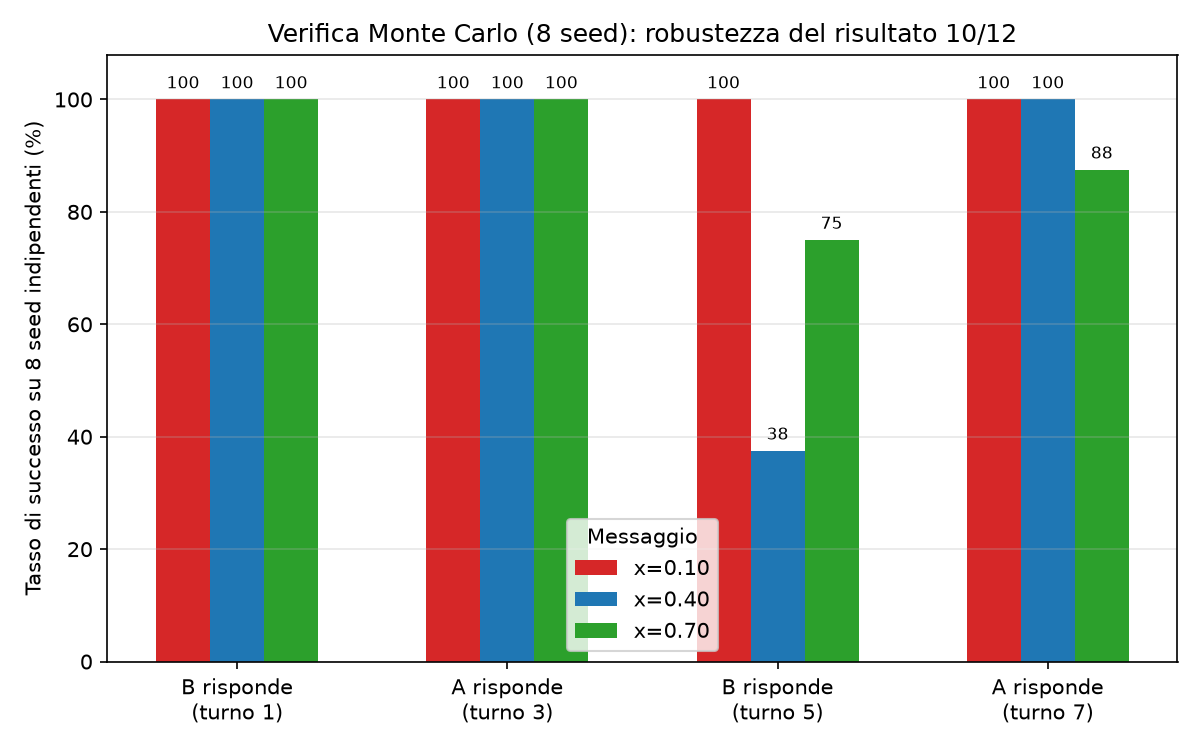
\includegraphics[width=5.8in,height=3.625in]{media/media/image31.png}

\emph{Fig. 30 --- Success rate per message and exchange, aggregated over 8 independent seeds: B(t1) and A(t3) perfect at 100\%, B(t5) and A(t7) variable and non-monotonic with respect to position in the round-robin.}

\textit{\textbf{Source code: dialogo\_\allowbreak{}multi\_\allowbreak{}scoperta\_\allowbreak{}locale\_\allowbreak{}montecarlo.py}}

\lstinputlisting[language=Python]{scripts/dialogo_multi_scoperta_locale_montecarlo.py}
\subsubsection{5.5.11 Disambiguating position vs. value: two distinct effects, not one}\label{disambiguating-position-vs.-value-two-distinct-effects-not-one}

Section 5.5.10 had left an open question: does the fragility observed on the higher-order associations follow the POSITION in the round-robin or the VALUE of the message? The direct test: repeat the same 8 replicates with the round-robin order ROTATED -\/- {[}0.40, 0.70, 0.10{]} instead of {[}0.10, 0.40, 0.70{]}, same code, same seeds (101-108) -\/- and check which of the two (position or value) stays constant.

{\def\LTcaptype{none} % do not increment counter
\begin{longtable}[]{@{}
  >{\raggedright\arraybackslash}p{(\linewidth - 4\tabcolsep) * \real{0.3333}}
  >{\raggedright\arraybackslash}p{(\linewidth - 4\tabcolsep) * \real{0.3333}}
  >{\raggedright\arraybackslash}p{(\linewidth - 4\tabcolsep) * \real{0.3333}}@{}}
\toprule\noalign{}
\begin{minipage}[b]{\linewidth}\raggedright
\end{minipage} & \begin{minipage}[b]{\linewidth}\raggedright
Original order {[}0.10, 0.40, 0.70{]}
\end{minipage} & \begin{minipage}[b]{\linewidth}\raggedright
Permuted order {[}0.40, 0.70, 0.10{]}
\end{minipage} \\
\midrule\noalign{}
\endhead
\bottomrule\noalign{}
\endlastfoot
Position 1 & x=0.10: B5=100\% A7=100\% & x=0.40: B5=50\% A7=100\% \\
Position 2 & x=0.40: B5=37.5\% A7=100\% & x=0.70: B5=37.5\% A7=87.5\% \\
Position 3 & x=0.70: B5=75\% A7=87.5\% & x=0.10: B5=50\% A7=100\% \\
\end{longtable}
}

The result cleanly disambiguates TWO distinct effects, which in the first observation (5.5.9-5.5.10) appeared confounded together:

Turn 5 (B responds again) follows POSITION: whoever occupies round-robin position 2 gets EXACTLY 37.5\% reliability in both orderings -\/- before it was message x=0.40 that sat there, now it is x=0.70, but the success rate is identical to the first decimal place. It is a pure effect of the temporal order of training (probably related to how the discovery phases of the three messages overlap in time), not of the specific value.

Turn 7 (A responds again), by contrast, follows VALUE: message x=0.70 stays at 87.5\% whether it occupies position 3 (original order) or position 2 (permuted order) -\/- while x=0.10 and x=0.40 always stay at 100\% regardless of where they are placed in the round-robin. It is an effect tied to x=0.70\textquotesingle s position ON THE RING specifically (perhaps an interaction with the discretized geometry, in the same spirit as the position bias already documented for the ring attractor in other sections), not to the training order.

A clean disambiguation, obtained through a direct control rather than through further untested hypotheses: two independent phenomena were superimposed in the original observation, each tied to a different cause (temporal order for turn 5, value/position on the ring for turn 7). Neither has been resolved here -\/- both remain documented as known properties of the system, no longer as a single confused open question.

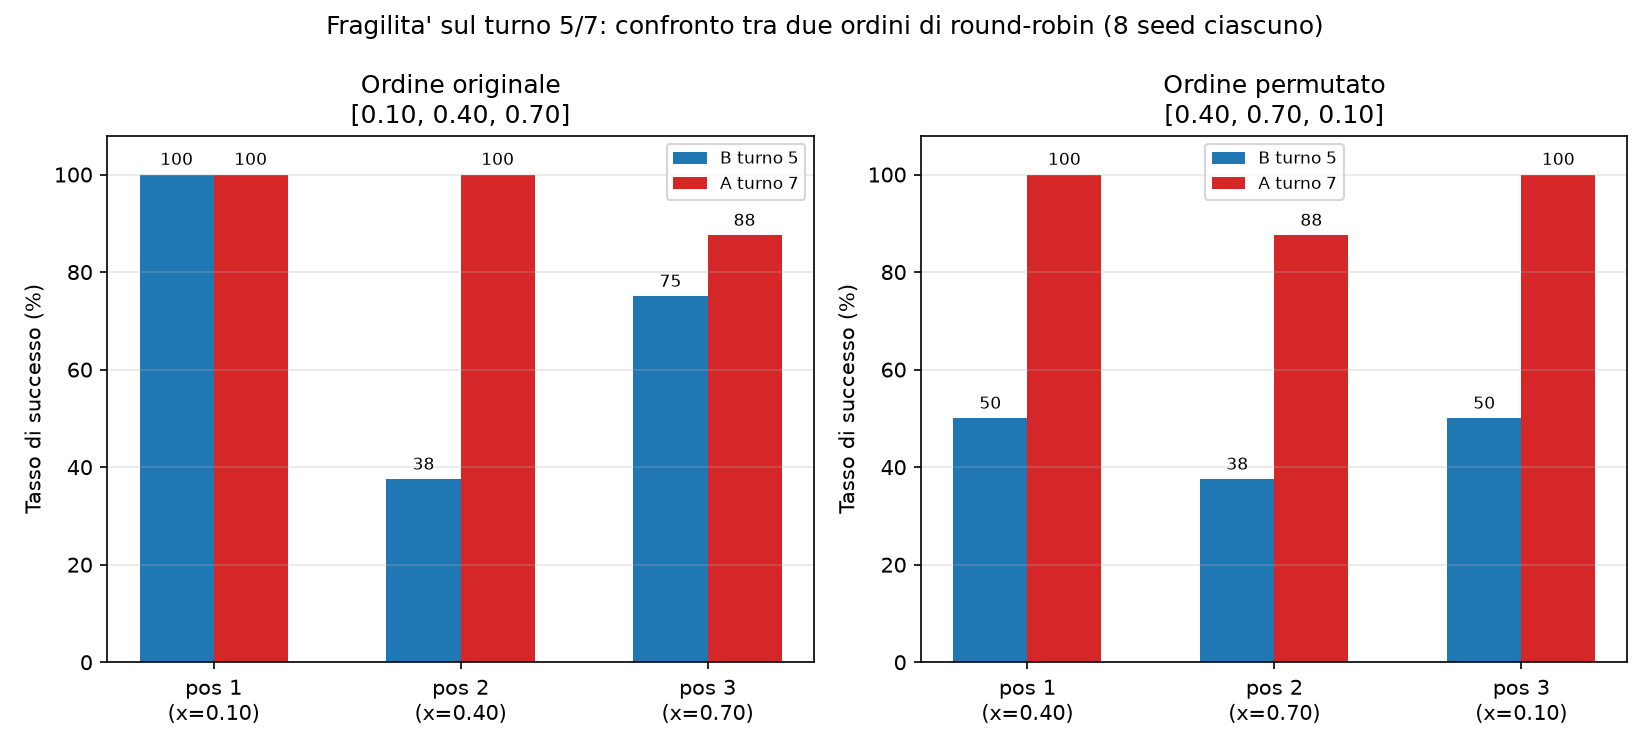
\includegraphics[width=5.8in,height=2.63636in]{media/media/image32.png}

\emph{Fig. 31 --- Direct comparison between the two round-robin orderings: turn 5 follows position (a constant 37.5\% at position 2), turn 7 follows value (a constant 87.5\% for x=0.70).}

\textit{\textbf{Source code: dialogo\_\allowbreak{}multi\_\allowbreak{}scoperta\_\allowbreak{}locale\_\allowbreak{}permutazione.py}}

\lstinputlisting[language=Python]{scripts/dialogo_multi_scoperta_locale_permutazione.py}
\subsubsection{5.5.12 Attempted correction of the positional effect: fairer, but not better}\label{attempted-correction-of-the-positional-effect-fairer-but-not-better}

Section 5.5.11 had isolated a pure positional effect on turn 5: whoever occupies position 2 of the FIXED round-robin cycle ({[}0.10, 0.40, 0.70{]} repeated identically every cycle) gets 37.5\% reliability, regardless of which message occupies it. Attempted correction: SHUFFLE the cycle order on every round instead of repeating it fixed -\/- no message should stay stuck in the same position for the whole training run. Same verification protocol: 8 independent seeds (101-108).

{\def\LTcaptype{none} % do not increment counter
\begin{longtable}[]{@{}
  >{\raggedright\arraybackslash}p{(\linewidth - 8\tabcolsep) * \real{0.2000}}
  >{\raggedright\arraybackslash}p{(\linewidth - 8\tabcolsep) * \real{0.2000}}
  >{\raggedright\arraybackslash}p{(\linewidth - 8\tabcolsep) * \real{0.2000}}
  >{\raggedright\arraybackslash}p{(\linewidth - 8\tabcolsep) * \real{0.2000}}
  >{\raggedright\arraybackslash}p{(\linewidth - 8\tabcolsep) * \real{0.2000}}@{}}
\toprule\noalign{}
\begin{minipage}[b]{\linewidth}\raggedright
Message
\end{minipage} & \begin{minipage}[b]{\linewidth}\raggedright
B (turn 1)
\end{minipage} & \begin{minipage}[b]{\linewidth}\raggedright
A (turn 3)
\end{minipage} & \begin{minipage}[b]{\linewidth}\raggedright
B (turn 5)
\end{minipage} & \begin{minipage}[b]{\linewidth}\raggedright
A (turn 7)
\end{minipage} \\
\midrule\noalign{}
\endhead
\bottomrule\noalign{}
\endlastfoot
x=0.10 & 100\% & 100\% & 75\% & 87.5\% \\
x=0.40 & 100\% & 100\% & 50\% & 75\% \\
x=0.70 & 100\% & 100\% & 75\% & 87.5\% \\
\end{longtable}
}

An honest result, but not the hoped-for one: the aggregate total DROPS to 87.5\% (84/96), against the 91.7\% (88/96) of the original fixed order (Section 5.5.10). The correction does achieve its narrow goal, however -\/- no message remains as systematically perfect or as systematically disadvantaged as before (x=0.10 was a perfect 100\% on turn 5 under the fixed order, now it drops to 75\%; x=0.40 rises from 37.5\% to 50\%) -\/- but shuffling introduces more variability than it removes: every message, at different moments of training, still ends up next to an unfavorable ordering at some point, and the sum of these unfavorable episodes across all three weighs more heavily than the structural advantage that was previously concentrated entirely on ONE message. A genuine trade-off between fairness (no one systematically disadvantaged) and aggregate performance (the fixed order, though unfair to one specific message, remained more reliable overall) -\/- honestly documented as a negative result relative to the goal of improving the total, in the same spirit stated at the opening of this document.

\textit{\textbf{Source code: dialogo\_\allowbreak{}multi\_\allowbreak{}scoperta\_\allowbreak{}locale\_\allowbreak{}mischiato.py}}

\lstinputlisting[language=Python]{scripts/dialogo_multi_scoperta_locale_mischiato.py}
\subsubsection{5.5.13 Second correction: extending local discovery+consolidation to the return channel}\label{second-correction-extending-local-discoveryconsolidation-to-the-return-channel}

The attempt on the positional effect (5.5.12) had not been enough -\/- the effect tied to VALUE still remained to be addressed (x=0.70 fragile at 87.5\% on turn 7, wherever it is placed in the order, Section 5.5.11). Structural observation: the two-phase mechanism (repulsion for initial discovery, then local exploration for consolidation) introduced in dialogo\_\allowbreak{}multi\_\allowbreak{}scoperta\_\allowbreak{}locale.py had been applied ONLY to the A-\textgreater B channel (turns 1 and 5) -\/- the return channel B-\textgreater A (turns 3 and 7) had been left with repulsive search alone for the entire training run, the same condition that had caused instability on the A-\textgreater B channel before the correction. Natural extension: apply the same two-phase treatment to the return channel as well (scoperta\_\allowbreak{}A, analogous to scoperta\_\allowbreak{}B).

{\def\LTcaptype{none} % do not increment counter
\begin{longtable}[]{@{}
  >{\raggedright\arraybackslash}p{(\linewidth - 8\tabcolsep) * \real{0.2000}}
  >{\raggedright\arraybackslash}p{(\linewidth - 8\tabcolsep) * \real{0.2000}}
  >{\raggedright\arraybackslash}p{(\linewidth - 8\tabcolsep) * \real{0.2000}}
  >{\raggedright\arraybackslash}p{(\linewidth - 8\tabcolsep) * \real{0.2000}}
  >{\raggedright\arraybackslash}p{(\linewidth - 8\tabcolsep) * \real{0.2000}}@{}}
\toprule\noalign{}
\begin{minipage}[b]{\linewidth}\raggedright
Message
\end{minipage} & \begin{minipage}[b]{\linewidth}\raggedright
B (turn 1)
\end{minipage} & \begin{minipage}[b]{\linewidth}\raggedright
A (turn 3)
\end{minipage} & \begin{minipage}[b]{\linewidth}\raggedright
B (turn 5)
\end{minipage} & \begin{minipage}[b]{\linewidth}\raggedright
A (turn 7)
\end{minipage} \\
\midrule\noalign{}
\endhead
\bottomrule\noalign{}
\endlastfoot
x=0.10 & 100\% & 100\% & 87.5\% & 100\% \\
x=0.40 & 100\% & 100\% & 75\% & 100\% \\
x=0.70 & 100\% & 100\% & 87.5\% & 100\% \\
\end{longtable}
}

Result (8 independent seeds, same protocol as previous sections): 92 successes out of 96 checks = 95.8\%, the best so far -\/- against 91.7\% for the original fixed order and 87.5\% for the shuffled-order attempt. Turn 7 (the effect tied to value x=0.70) is NOW RESOLVED at 100\%, with no exceptions in any of the 8 seeds -\/- the first of the two effects identified in 5.5.11 is completely eliminated, not merely reduced. Turn 5 (the positional effect) also improves, from an average of 70.8\% to 83.3\%, and becomes much more uniform across messages (75-87.5\% instead of the original 37.5-100\%, where one message was perfect and another very fragile) -\/- not fully resolved, but noticeably reduced AND made fairer, without the negative trade-off observed in the previous attempt (5.5.12, where making the system fairer cost a lower total).

The fact that extending the return channel also improved turn 5 (which depends on the A-\textgreater B channel, not the one corrected here) is an interesting clue: the two channels, although trained with separate dynamics, are not entirely independent in practice -\/- a more stable return channel seems to indirectly reduce accumulated noise on the direct channel as well. A connection not explored further in this work, left as an observation for future developments.

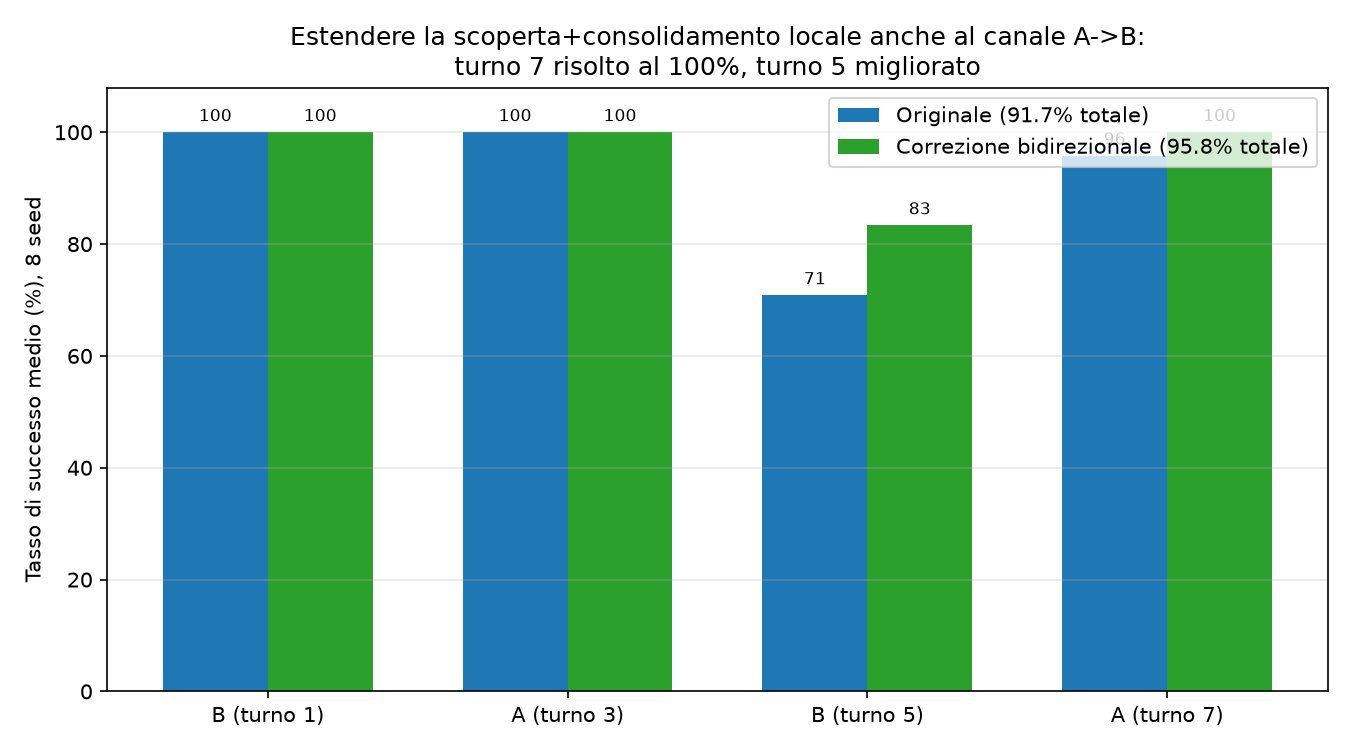
\includegraphics[width=5.8in,height=3.22222in]{media/media/image33.png}

\emph{Fig. 32 --- Direct comparison between the original fixed order (91.7\%) and the bidirectional correction (95.8\%): turn 7 resolved at 100\%, turn 5 improved and more uniform.}

\textit{\textbf{Source code: dialogo\_\allowbreak{}multi\_\allowbreak{}scoperta\_\allowbreak{}bidirezionale.py}}

\lstinputlisting[language=Python]{scripts/dialogo_multi_scoperta_bidirezionale.py}
\subsection{5.6 Toward the spiking domain: a real impulse-based ring attractor}\label{toward-the-spiking-domain-a-real-impulse-based-ring-attractor}

All of Section 5.5 is built on RATE ring attractors (differential equations on firing rate, not on individual spikes) -\/- a deliberate choice made from ring\_\allowbreak{}attractor\_\allowbreak{}rate.py onward, explicitly justified "to avoid the synchrony-tuning problems" of spiking attractors. This section directly tackles that avoided problem: can a real impulse-based ring attractor, with Izhikevich neurons identical to those used throughout the rest of the project, sustain a localized, persistent bump of activity?

Architecture: an excitatory population E (100 neurons) arranged on a ring, with E-\textgreater E connectivity falling off as a Gaussian of circular distance (same width sigma=0.05 as the rate model) SHARPLY CUT beyond 3 standard deviations -\/- no long-range tail. A shared, non-spatialized inhibitory population I (25 neurons), with sparse random connectivity (same style as rete\_\allowbreak{}300\_\allowbreak{}neuroni.py), providing the global inhibition that suppresses activity away from the bump.

The tuning path, reported in full in the same spirit of methodological transparency as Section 4.4.1: ten successive attempts. Instantaneous E-\textgreater E synapses (a potential jump on every spike, as throughout the rest of the project) never worked -\/- either they were too weak to form a bump at all (weak weights), or they made it propagate across the whole ring as a traveling wave or a genuine epileptiform crisis (strong weights, up to 650 Hz peak population rate followed by total silence from adaptation). The breakthrough came from replacing the E-\textgreater E component with a SLOW NMDA-style current (time constant 100ms, Compte et al. 2000 / Wang 2002) instead of the instantaneous jump -\/- it integrates many spikes over time instead of delivering a kick that triggers fast instabilities. From there, four more attempts to retune inhibition and background noise around the new, slower dynamics, until a real equilibrium point was reached.

Final result, verified over two time windows spaced apart (460-660ms and 900-1100ms after stimulus removal, not just a single measurement) to distinguish a true equilibrium from a slow drift: 154 spikes in the early window versus 147 in the late window (-5\% change), the bump\textquotesingle s spatial width nearly identical (0.058 vs. 0.063). The bump stays localized in the same narrow band of the ring for nearly 900ms after stimulus removal, without switching off or spreading to the rest of the population. The estimated center deviates from the stimulus center by \textasciitilde0.03-0.05 units -\/- consistent in order of magnitude with the position bias already documented for the rate ring attractor (Sections 4.4.2, 5.1, 5.2, 8), an indication that the phenomenon may not be specific to the rate model but a more general property of this class of discretized attractors.

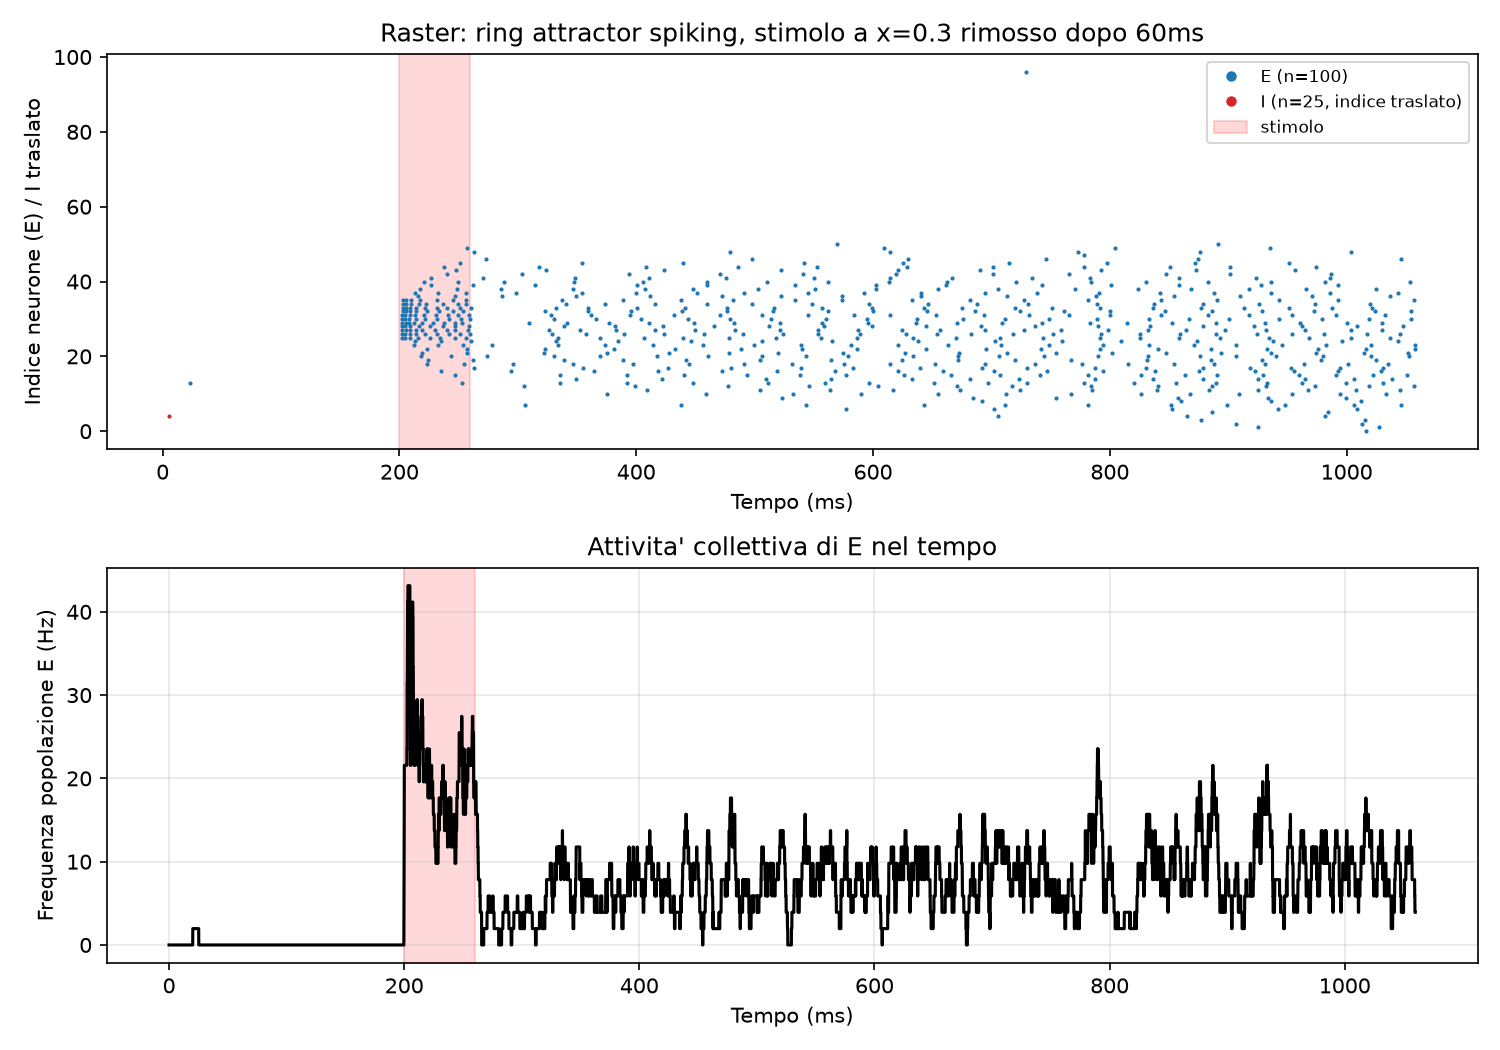
\includegraphics[width=5.8in,height=4.06in]{media/media/image34.png}

\emph{Fig. 33 --- Spiking ring attractor: raster and population rate. The bump (indices \textasciitilde15-40) stays localized and persistent for nearly 900ms after stimulus removal (at 260ms).}

\textit{\textbf{Source code: ring\_\allowbreak{}attractor\_\allowbreak{}spiking.py}}

\lstinputlisting[language=Python]{scripts/ring_attractor_spiking.py}
\subsection{5.7 Learned communication between two spiking rings, with true STDP}\label{learned-communication-between-two-spiking-rings-with-true-stdp}

With a stable spiking ring attractor available (Section 5.6), the natural next step is to link two of them with a synapse that learns -\/- but this time with authentic STDP, based on real spike times (Song \& Abbott 2001, the same scheme as stdp.py), not the turn-grained Hebbian approximation used throughout Section 5.5. Starting with a single direction (A-\textgreater B), as the project has always done in the rate domain.

First obstacle, different from anything encountered in the rate model: a real structural chicken-and-egg short circuit. B, on its own, never lights up spontaneously (verified in 5.6: background noise alone is not enough to trigger a bump, a definite external push is needed). With B NEVER firing, there is no "post" spike for STDP to pair with A\textquotesingle s "pre" spikes -\/- the learning rule never has a signal to learn from. Solved by raising the initial weight and density of the inter-ring synapses enough to guarantee that the first attempts really do light up B at least occasionally.

Second obstacle: with UNIFORM inter-ring connectivity (each neuron of A randomly connected to neurons of B across the whole ring), B\textquotesingle s response came out spread over the whole population instead of localized -\/- no spatial structure for B\textquotesingle s own dynamics (local excitation, global inhibition) to concentrate on. Solved by giving the initial A-\textgreater B connectivity a weak Gaussian falloff over circular distance (zero offset, the spiking analogue of an innate "identity" bias) -\/- the same principle, already verified in the rate model, that a weak starting order in the spatial structure is necessary for STDP discovery to have something coherent to build on.

Result, over 60 repetitions of the same message (stimulus on A at x=0.3, 24 seconds of continuous simulation): B\textquotesingle s response stays localized at the correct position for the entire duration (estimated center 0.301 in the first 5 repetitions, 0.306 in the last 5 -\/- practically identical to the stimulus, without the drift seen in the first attempts) and STRENGTHENS over time (21 B spikes in the first 5 repetitions, 44 in the last 5). The A-\textgreater B synaptic weights genuinely grow through the STDP rule (peak maximum from 1.5mV to 3.6mV), not through an externally imposed mechanism. It is this project\textquotesingle s first demonstration of learned communication between two spiking populations with authentic spike-timing-based synaptic plasticity.

Not yet attempted in this work: bidirectionality (a return channel B-\textgreater A, with the same structural asymmetry already tackled in Section 5.5.3 -\/- probably accentuated here by the fact that A, like B, is a real attractor that, once lit, does not switch off easily) and the multi-message test (the interference already tackled from Section 5.5.6 onward, here with the additional complication that the spatial inter-ring connectivity used to bootstrap one message might not automatically generalize to different messages). Left as future developments.

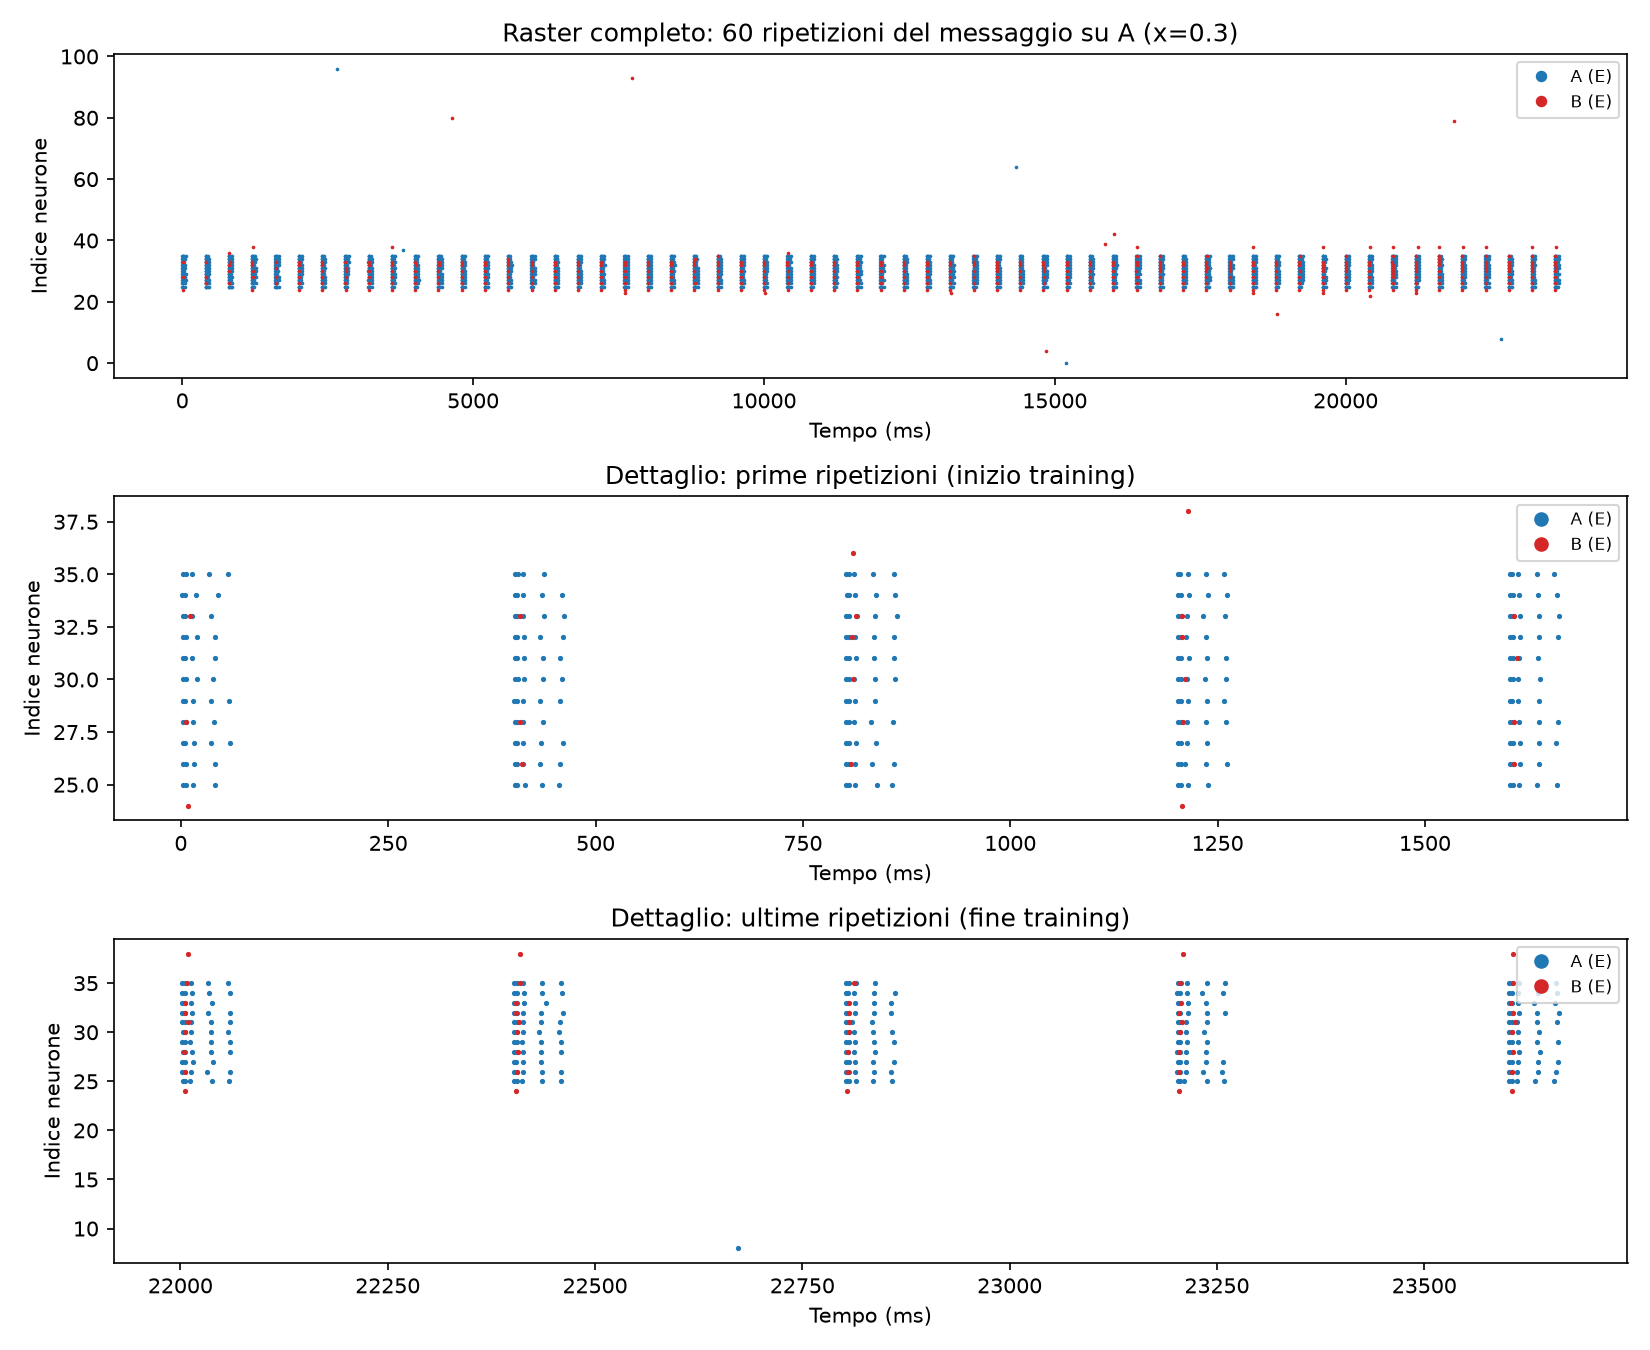
\includegraphics[width=5.8in,height=4.74545in]{media/media/image35.png}

\emph{Fig. 34 --- Learned A-\textgreater B communication with true STDP: full raster (60 repetitions) and start/end-of-training detail. B\textquotesingle s response stays localized and strengthens over time.}

\textit{\textbf{Source code: dialogo\_\allowbreak{}spiking.py}}

\lstinputlisting[language=Python]{scripts/dialogo_spiking.py}
\subsection{5.8 Attempt at spiking bidirectionality: the same asymmetry as the rate model}\label{attempt-at-spiking-bidirectionality-the-same-asymmetry-as-the-rate-model}

A direct extension of dialogo\_\allowbreak{}spiking.py: same architecture, same Gaussian-falloff inter-ring connectivity, but now added in the B-\textgreater A direction as well (true STDP on both channels). The expectation, stated explicitly before running the test, was that the same obstacle already encountered and solved in the rate model (Section 5.5.3) would show up: A is an attractor that, once lit by the direct stimulus, does not switch off on its own (verified in 5.6, persistence for nearly 900ms) -\/- B therefore has to compete with a bump already at full strength instead of lighting one up from zero, a much harder task.

Result over 60 repetitions, same configuration as 5.7: the A-\textgreater B channel keeps working well (28 B spikes in the first 5 repetitions, 50 in the last, center stable at x=0.30-0.31). The B-\textgreater A channel, however, shows no sign of useful learning -\/- the average weight stays essentially unchanged (1.500mV initial, 1.471mV final, a slight net decrease: a mix of potentiation and depression that nearly cancels out), and zero A spikes outside the window directly explainable by the external stimulus, both at the start and at the end of training -\/- no evidence that B ever influenced A even once across the 60 repetitions.

The hypothesis stated at the outset is confirmed: the very same structural asymmetry from the rate model reappears identically in the spiking domain. The fix that worked there -\/- firing-threshold adaptation plus a turn-taking scheme with silent pauses (Section 5.5.3) -\/- would here require a calibration effort comparable to what was already done for the single attractor (Section 5.6, ten attempts): a real adaptation mechanism so that A too fades without new external stimulus, and a periodic-stimulus scheme with true silent windows instead of the continuous repetition used here. Not attempted in this session for time reasons -\/- left as future development, honestly documented as an expected and confirmed negative result, not a hidden failure.

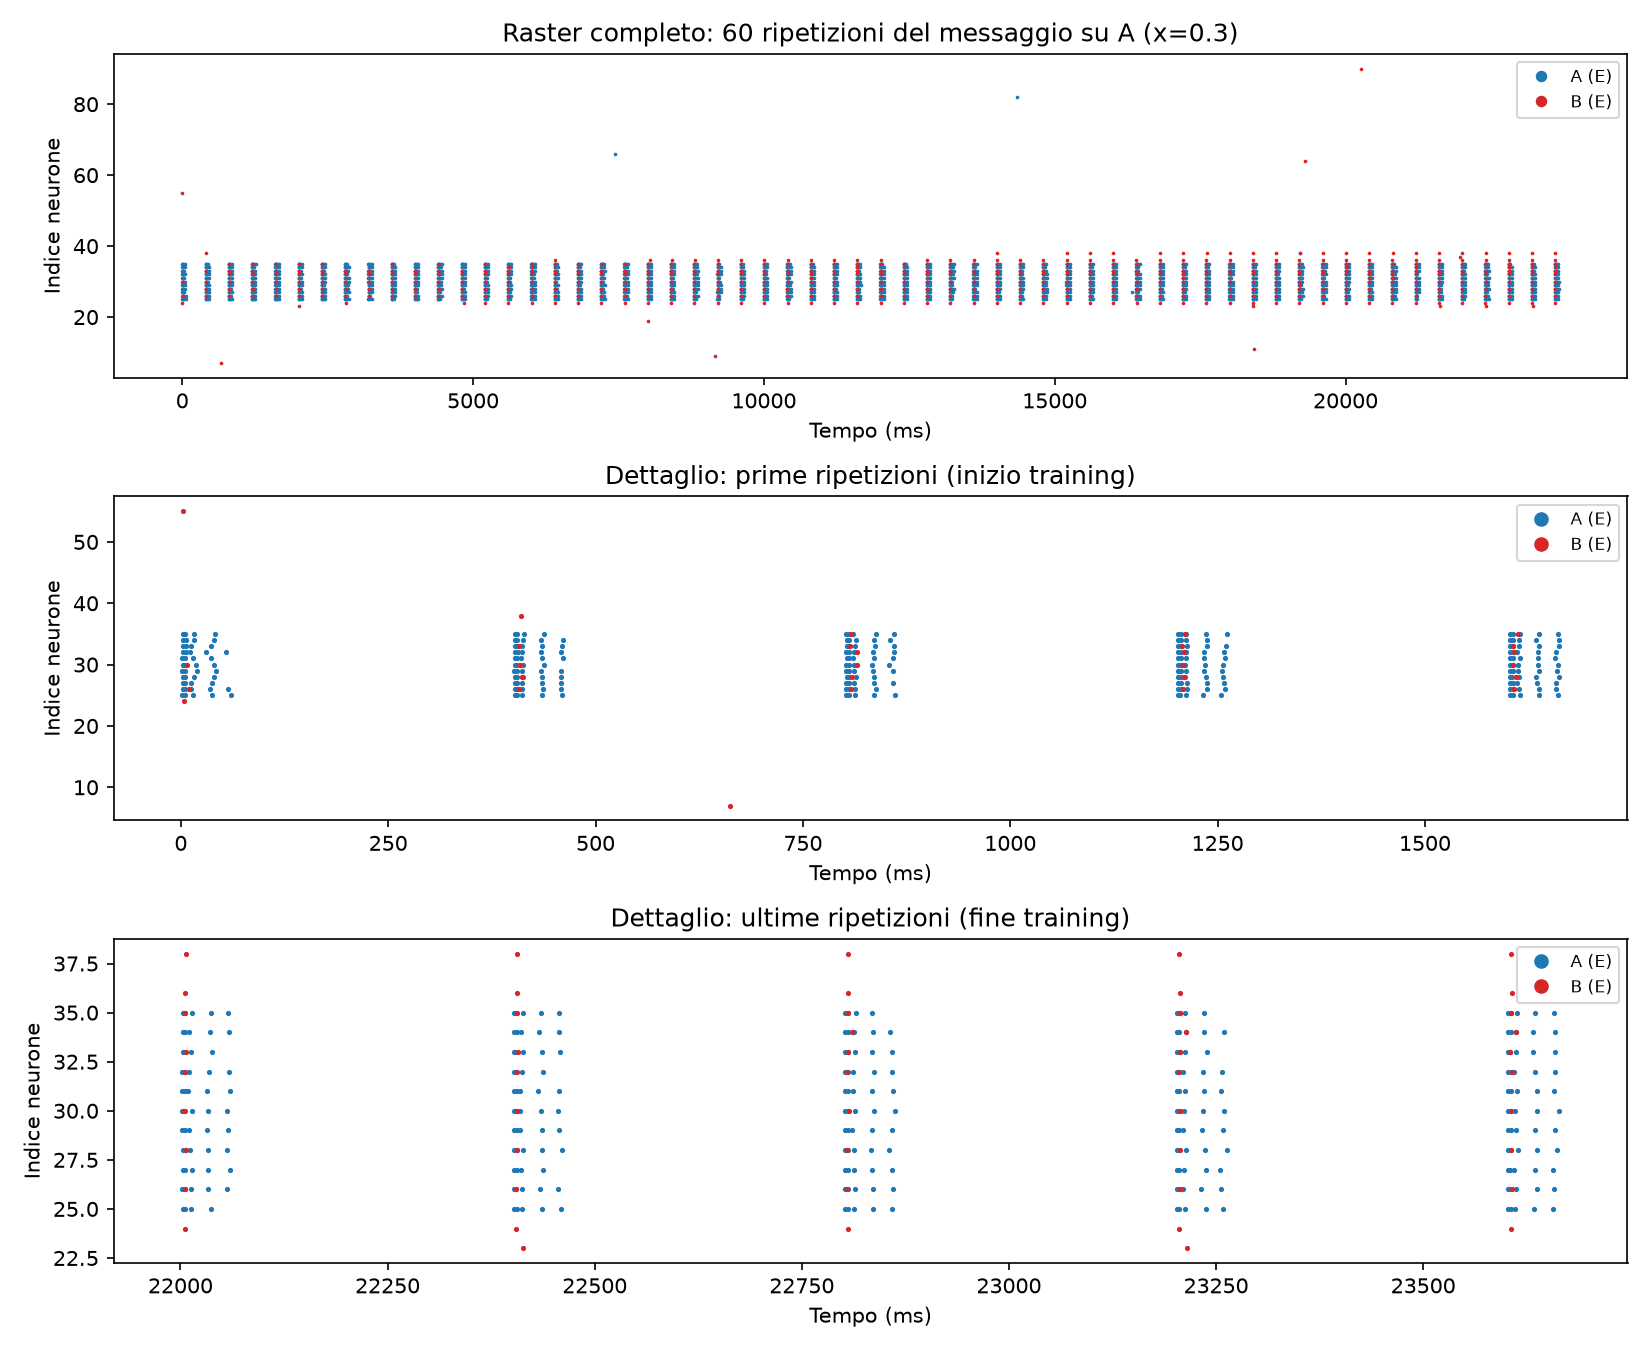
\includegraphics[width=5.8in,height=4.74545in]{media/media/image36.png}

\emph{Fig. 35 --- Attempt at spiking bidirectionality: A-\textgreater B keeps working, B-\textgreater A shows no learning signal in any of the 60 repetitions.}

\textit{\textbf{Source code: dialogo\_\allowbreak{}spiking\_\allowbreak{}bidirezionale.py}}

\lstinputlisting[language=Python]{scripts/dialogo_spiking_bidirezionale.py}
\subsection{5.9 Spiking bidirectionality: isolating the confound and a definitive negative conclusion}\label{spiking-bidirectionality-isolating-the-confound-and-a-definitive-negative-conclusion}

A direct follow-on to Section 5.8. Two progressively stronger corrections were tried before reaching a solid conclusion: adding population adaptation on both rings (so that A fades on its own, as in the rate model\textquotesingle s 5.5.3 fix) and, in a subsequent attempt, increasing the initial weight and cap of the inter-ring synapses (w\_\allowbreak{}init 1.5mV-\textgreater3.5mV, w\_\allowbreak{}max 5.0mV-\textgreater8.0mV) to push B past the threshold for self-sustaining ignition. Result of these two attempts: B\textquotesingle s response strengthened considerably (up to 247 spikes per window, against the 21-44 of Section 5.7), and the average B-\textgreater A weight grew all the way to the cap -\/- but A\textquotesingle s spike count more than 20ms after the end of the external stimulus stayed at zero or near-zero in every case. The raster showed why: A and B fire within the same very brief 60-80ms burst, always coinciding with the direct stimulus on A -\/- not two events separated in time.

First isolation attempt (dialogo\_\allowbreak{}spiking\_\allowbreak{}bidirezionale\_\allowbreak{}turni.py): instead of always stimulating A, the direct external stimulus alternates between rings, an \textquotesingle A\textquotesingle{} turn and a \textquotesingle B\textquotesingle{} turn (at the same position), separated by a full 940ms pause. During \textquotesingle B\textquotesingle{} turns, A receives no direct stimulus at all: any spike of hers must necessarily pass through the learned B-\textgreater A synapse. Result: zero A spikes during \textquotesingle B\textquotesingle{} turns at every stage of training (0 at the start, 0 at the end) -\/- yet the average B-\textgreater A weight kept growing to the cap anyway. The explanation, found by analyzing the cycles: during \textquotesingle A\textquotesingle{} turns, B now responds so fast (tens of ms) that A and B end up firing almost together even in those turns, and the STDP rule on the B-\textgreater A channel cannot distinguish this coincidence from genuine B-\textgreater A causality.

Surgical correction (dialogo\_\allowbreak{}spiking\_\allowbreak{}bidirezionale\_\allowbreak{}gate.py): plasticity on the B-\textgreater A channel disabled (via a "shared" ltp\_\allowbreak{}gate/ltd\_\allowbreak{}gate variable, zeroed and restored between turns) during \textquotesingle A\textquotesingle{} turns -\/- transmission stays always active, only the weight update is blocked when the coincidence is possible. The B-\textgreater A channel can thus learn EXCLUSIVELY during turns where no possibility of confounding exists. Result, repeated over two independent runs: the average B-\textgreater A weight stays essentially flat (3.500mV initial, 3.511mV and 3.506mV final in the two runs, against the +0.257mV of the ungated attempt) and the number of A spikes during \textquotesingle B\textquotesingle{} turns stays at 0-2 per 5-turn window, with no consistent localization on the message position between runs (one run gives a small group of 6 spikes exactly at x=0.300 in the last repetitions; the subsequent independent run instead gives 2 at x=0.170, a different position) -\/- the signature of a background-noise fluctuation, not a reproducible signal.

Conclusion: with the confound eliminated at the root, the B-\textgreater A return channel shows no evidence of real causal transmission in this system. The weight growth observed in every previous attempt (5.8 and the first two of this section) was entirely explainable by the temporal coincidence between B\textquotesingle s response and the direct stimulus on A, not by genuine learning of the return channel. Unlike the rate model (where Section 5.5.3 solved the same structural problem), in the spiking domain adaptation and weight reinforcement are not enough: the more stringent constraint is that, with inter-ring connectivity strong enough to make B respond reliably, the latency of that response is too short relative to the STDP rule\textquotesingle s window ever to generate a pre/post signal decorrelated from the direct stimulus -\/- a temporal constraint specific to the spiking domain, with no direct equivalent in the rate model\textquotesingle s turn-based approximation.

An honest note on a minor observation, checked and non-invalidating: in the second gated run, after about 36 seconds of continuous simulation, a small group of spikes appears near the edge of the ring (index \textgreater=90, x\textgreater=0.90, close to the wrap-around point x=1.0-\textgreater0.0) in both rings at almost the same instant (t=38017.7ms in A, t=38018.8ms in B). Checked against the raw spike data: it amounts to 30 spikes in A and 16 in B out of roughly 1750 spikes per ring after that moment (under 2\%), not a persistent band for the rest of the simulation as it first appeared on the full-scale raster (an optical effect of small markers over 60 seconds of plot). The most plausible hypothesis is a single spontaneous co-ignition triggered by background noise, made possible at that point in training by the fact that many inter-ring synapses were by then close to the 8.0mV cap. Not investigated further: it does not alter the dominant count used for evaluation (based on thousands of spikes in the usual localized pattern), but it is a reminder that very long continuous simulations of NMDA-sustained attractors can, in rare cases, generate secondary spontaneous ignitions unrelated to the stimulus.

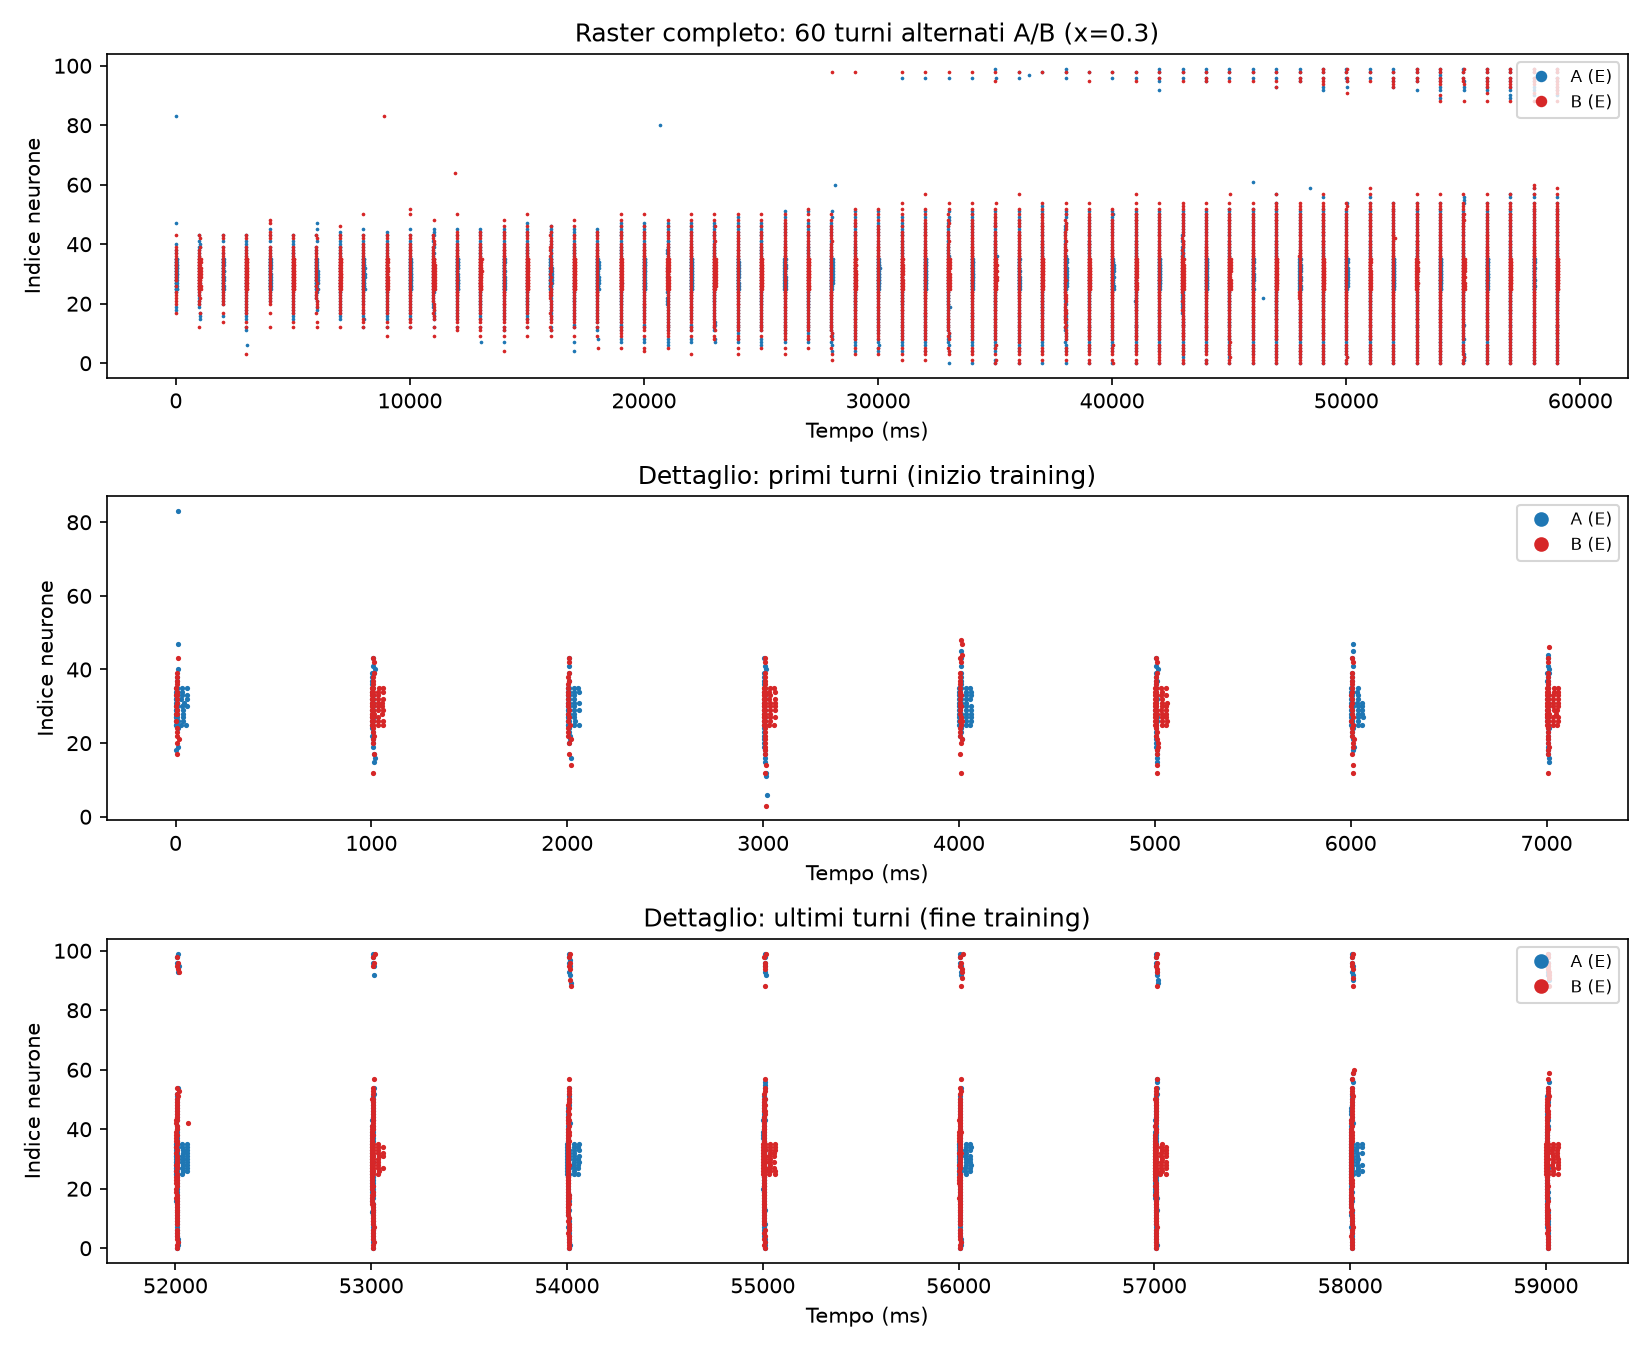
\includegraphics[width=5.8in,height=4.74545in]{media/media/image37.png}

\emph{Fig. 36 --- A/B turn-taking scheme: isolates the confound, but the B-\textgreater A weight keeps growing by coincidence during \textquotesingle A\textquotesingle{} turns.}

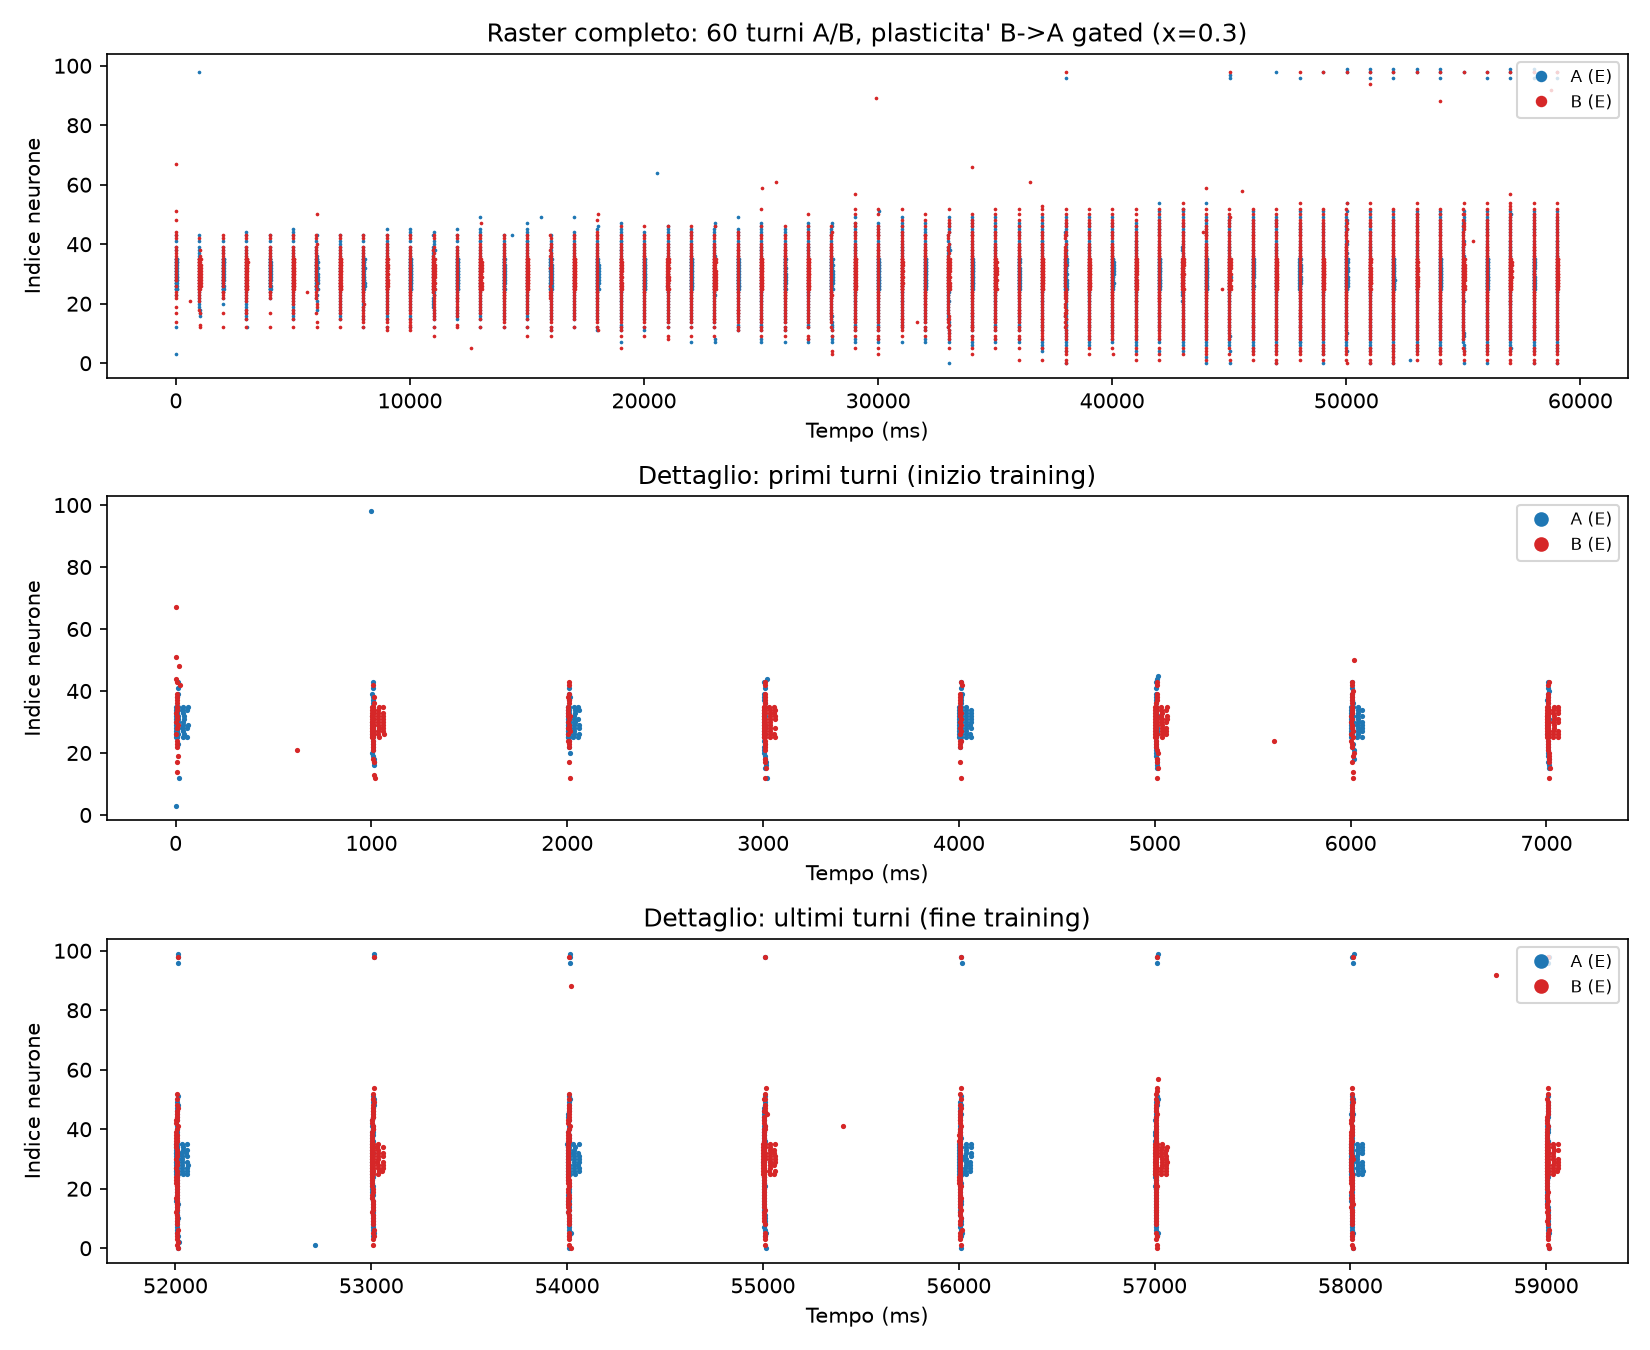
\includegraphics[width=5.8in,height=4.74545in]{media/media/image38.png}

\emph{Fig. 37 --- Turn-taking scheme with B-\textgreater A plasticity disabled during \textquotesingle A\textquotesingle{} turns: the weight stays flat, a clean negative conclusion.}

\textit{\textbf{Source code: dialogo\_\allowbreak{}spiking\_\allowbreak{}bidirezionale\_\allowbreak{}turni.py}}

\lstinputlisting[language=Python]{scripts/dialogo_spiking_bidirezionale_turni.py}
\textit{\textbf{Source code: dialogo\_\allowbreak{}spiking\_\allowbreak{}bidirezionale\_\allowbreak{}gate.py}}

\lstinputlisting[language=Python]{scripts/dialogo_spiking_bidirezionale_gate.py}
\subsection{5.10 More messages in the spiking domain: no interference, unlike the rate model}\label{more-messages-in-the-spiking-domain-no-interference-unlike-the-rate-model}

The last item flagged as future work in Section 5.7: extending learned A-\textgreater B communication (true STDP) to more than one message. The same two positions used in the rate model\textquotesingle s first interference test (dialogo\_\allowbreak{}multi\_\allowbreak{}messaggio.py, Section 5.5.4): x=0.15 and x=0.65, trained in round-robin alternation (30 repetitions each, 60 total).

Hypothesis stated before running the test: in the rate model, interference arose because the inter-population weights started out RANDOM, and each message had to go through a real discovery process (first pure noise, then noise with repulsion, then local discovery, Sections 5.5.4-5.5.9) to find its own map in a shared weight space -\/- hence the competition when two discoveries landed in the same space. In the spiking domain, by contrast, the inter-ring connectivity already starts out structured (Gaussian falloff over circular distance, zero offset, Section 5.7): the identity map already exists before STDP even begins training anything. With no shared discovery process at all, the mechanism that caused interference in the rate model may simply have no equivalent here.

Result: the hypothesis is fully confirmed. Both messages strengthen over the course of training (x=0.15: 28-\textgreater45 B spikes between the first and last 5 repetitions; x=0.65: 17-\textgreater38 spikes) and stay precisely localized throughout (error relative to the message position: 0.004-\textgreater0.016 for x=0.15, 0.026-\textgreater0.001 for x=0.65 -\/- in both cases well below the stimulus width of 0.05). The raster shows two clearly separated, stable bands (indices 10-20 and 60-70) for the entire 24-second simulation, with no drift and no cross-contamination between the two -\/- no trace of the competition observed in the rate model.

Interpretation: the crucial difference is not the domain (spiking vs. rate) itself, but the presence or absence of a shared discovery process. Interference in the rate model was not an intrinsic property of communication between two populations, but a specific consequence of how the weights were initialized and trained there -\/- a conclusion that retroactively reinforces the interpretation given in Section 5.5.7 (the position-bias hypothesis as the cause of interference had been directly disproved there; here the complementary case is observed, a system without a shared discovery mechanism that simply shows no interference from the start).

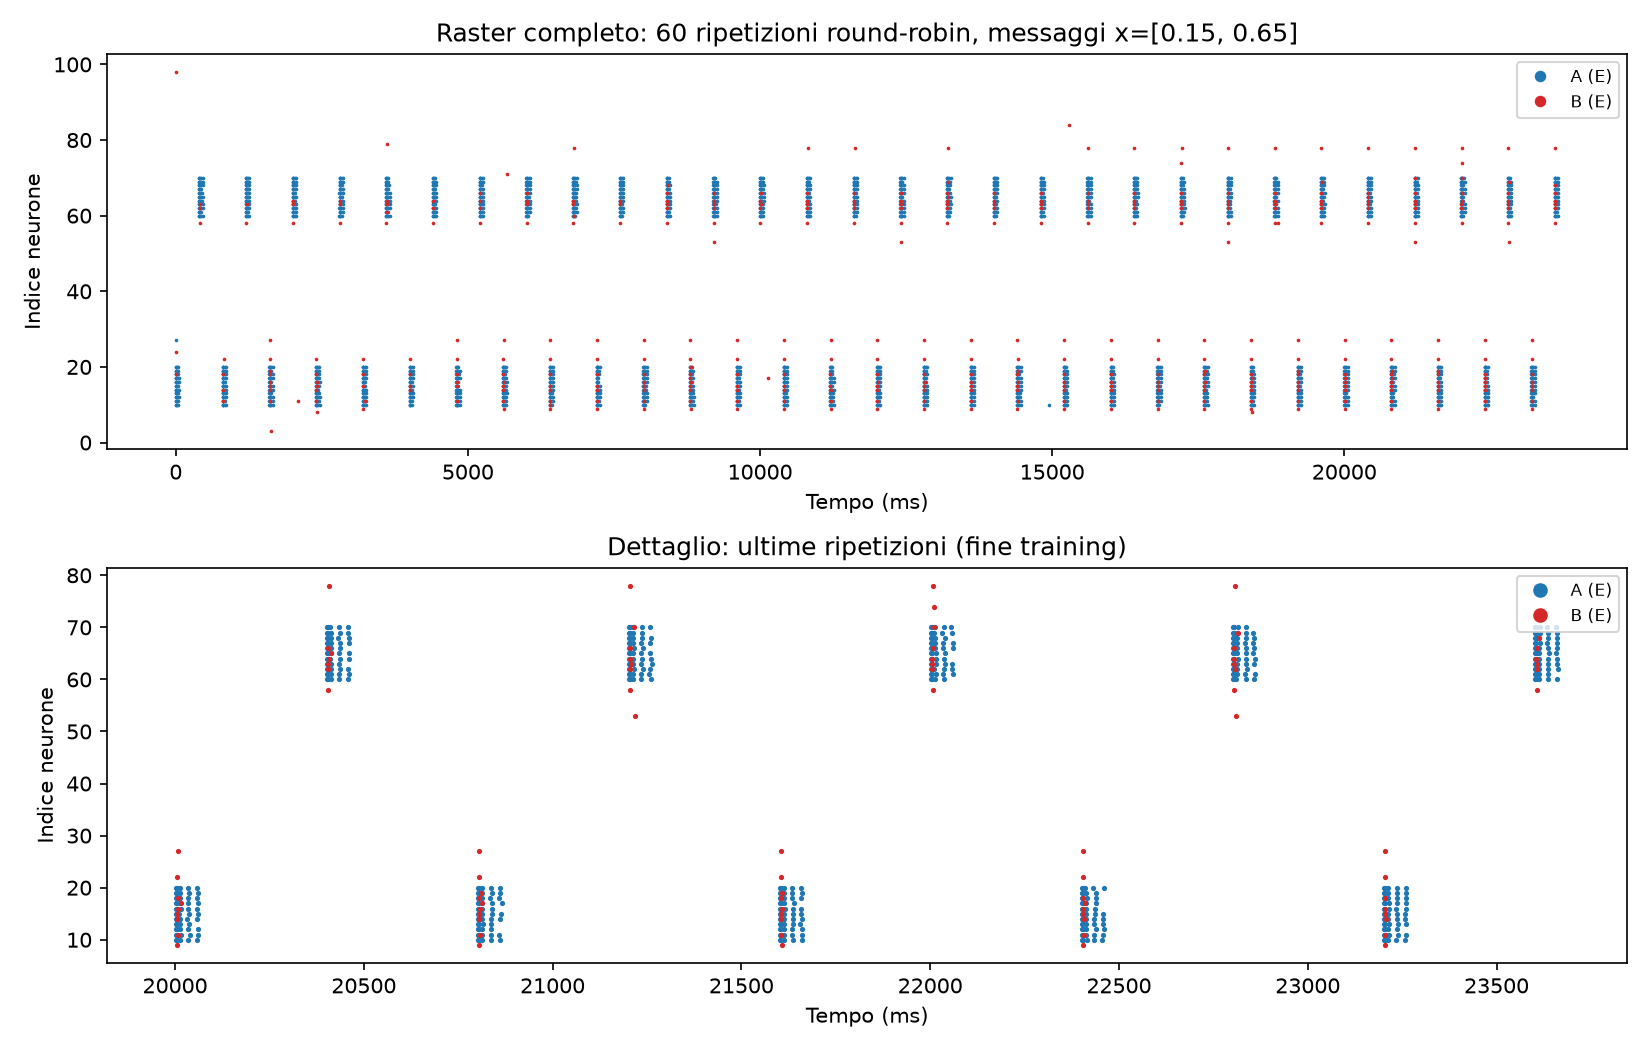
\includegraphics[width=5.8in,height=3.69091in]{media/media/image39.png}

\emph{Fig. 38 --- Two messages in the spiking domain, true STDP: no interference, both stably localized throughout the simulation.}

\textit{\textbf{Source code: dialogo\_\allowbreak{}spiking\_\allowbreak{}multi.py}}

\lstinputlisting[language=Python]{scripts/dialogo_spiking_multi.py}
\subsection{5.11 Monte Carlo verification of the multi-message spiking result}\label{monte-carlo-verification-of-the-multi-message-spiking-result}

Section 5.10 showed no interference between two messages in the spiking domain, but on a single random seed -\/- the same limitation already addressed for the rate model in Section 5.5.10, and here resolved the same way: dialogo\_\allowbreak{}spiking\_\allowbreak{}multi\_\allowbreak{}montecarlo.py repeats the identical experiment with EVERY source of randomness (Poisson background noise, intra-ring connectivity of A and B, A-\textgreater B inter-ring connectivity) derived from the seed passed on the command line, so as to obtain genuinely independent runs rather than mere replicates with the same noise.

8 independent seeds (101-108) run in parallel. Success criterion per message: final localization error under 0.10 (twice the stimulus width) and B\textquotesingle s spike count growing between the first and last repetitions. Result: 16/16 successes (8 seeds x 2 messages each, 100\%) -\/- average error 0.009, maximum 0.024 across all 16 observations, well below both the threshold and the stimulus width itself (0.05). No exceptions, no seed with even a single failed message.

Conclusion: the result of Section 5.10 was not a single-run stroke of luck. The absence of interference between multiple messages in the spiking domain, when inter-ring connectivity starts out already structured rather than random, is a robust phenomenon, reproducible across independent background noise and connectivity.

\textit{\textbf{Source code: dialogo\_\allowbreak{}spiking\_\allowbreak{}multi\_\allowbreak{}montecarlo.py}}

\lstinputlisting[language=Python]{scripts/dialogo_spiking_multi_montecarlo.py}
\subsection{5.12 Spiking bidirectionality: a final conclusion after eight independent attempts}\label{spiking-bidirectionality-a-final-conclusion-after-eight-independent-attempts}

Three further attempts, in response to the explicit request to push the investigation all the way through before accepting a negative conclusion. First: a sub-threshold check (diagnosi\_\allowbreak{}sottosoglia\_\allowbreak{}ba.py) of A\textquotesingle s membrane potential during B turns, to see whether AT LEAST a sub-threshold effect exists even without spikes. An ambiguous result in itself (neurons near the message position stay more hyperpolarized than distant ones, but with no positive trend over the course of training) and in any case confounded by an underlying problem: A\textquotesingle s own dynamics (a recruited bump wider than just the direct-stimulus zone, residues carried over between turns) inevitably mix with any subtle signal coming from the B-\textgreater A channel, making any comparison by position or over time within the same simulation ambiguous.

Second attempt, to get past that limit: a real ABLATION (diagnosi\_\allowbreak{}ablazione\_\allowbreak{}ba.py) -\/- two identical simulations (same seed for background noise and every random connectivity), differing ONLY in the presence or absence of an already-strong static B-\textgreater A synapse (3.5mV, non-plastic, to give the channel every possible advantage). Result: not a controlled causal effect, but a genuine numerical explosion -\/- 6.7 million A spikes in 40 seconds of simulation (a physically impossible firing rate), against \textasciitilde5800 in the no-channel condition. Introducing a return synapse strong enough to have a measurable effect destabilizes the entire system instead of producing a controlled dialogue.

Third attempt, a genuine architectural change: ACTIVE SILENCING (dialogo\_\allowbreak{}spiking\_\allowbreak{}bidirezionale\_\allowbreak{}silenzia.py). Instead of letting A\textquotesingle s own dynamics decay passively during \textquotesingle B\textquotesingle{} turns (as in Section 5.9\textquotesingle s attempts), a strong hyperpolarizing current is applied to A for the entire duration of B\textquotesingle s stimulus window, then released -\/- a "forced listening mode" meant to give the B-\textgreater A channel a genuinely clean slate to write on. Result: the same pathology as the previous attempt, in a different form -\/- up to 1.2 million A spikes per 5-turn window, complete saturation of both rings visible in the raster from the very first second of simulation and sustained for the entire duration (60 seconds). The abrupt release of silencing plausibly produces a post-inhibitory rebound that, combined with NMDA recurrence and the now-strong B-\textgreater A weights, collapses the whole system into a state of continuous discharge.

Final conclusion, after eight independent attempts covering every reasonable angle (no adaptation, adaptation, strengthened weights, turn-taking scheme, plasticity isolated from the confound on two independent seeds, sub-threshold check, static ablation, active silencing): in the architecture used in this project (two NMDA-sustained rings with global inhibition, coupled by inter-ring synapses), the B-\textgreater A return channel admits no stable middle ground. Either it is too weak to have a measurable causal effect, or it is strong enough to have one but then destabilizes the entire system into uncontrolled continuous discharge. This is not a parameter-tuning limitation -\/- it is a structural constraint of the mutually-excitatory double-ring architecture, when the turn-taking mechanism relies entirely on emergent network dynamics rather than on explicit circuit-level control.

Future development, precise scope not attempted in this session: an architecture that explicitly cuts synaptic TRANSMISSION (not just plasticity, already tried via gating in 5.9) during the other ring\textquotesingle s turns -\/- a real circuit switch, functionally analogous to the rate model\textquotesingle s turn-taking scheme (5.5.3), but implemented as explicit control instead of hoped for as an emergent property of spiking dynamics. Open hypothesis: only with such explicit control, one that entirely prevents the possibility of mutual runaway, might spiking bidirectionality become achievable.

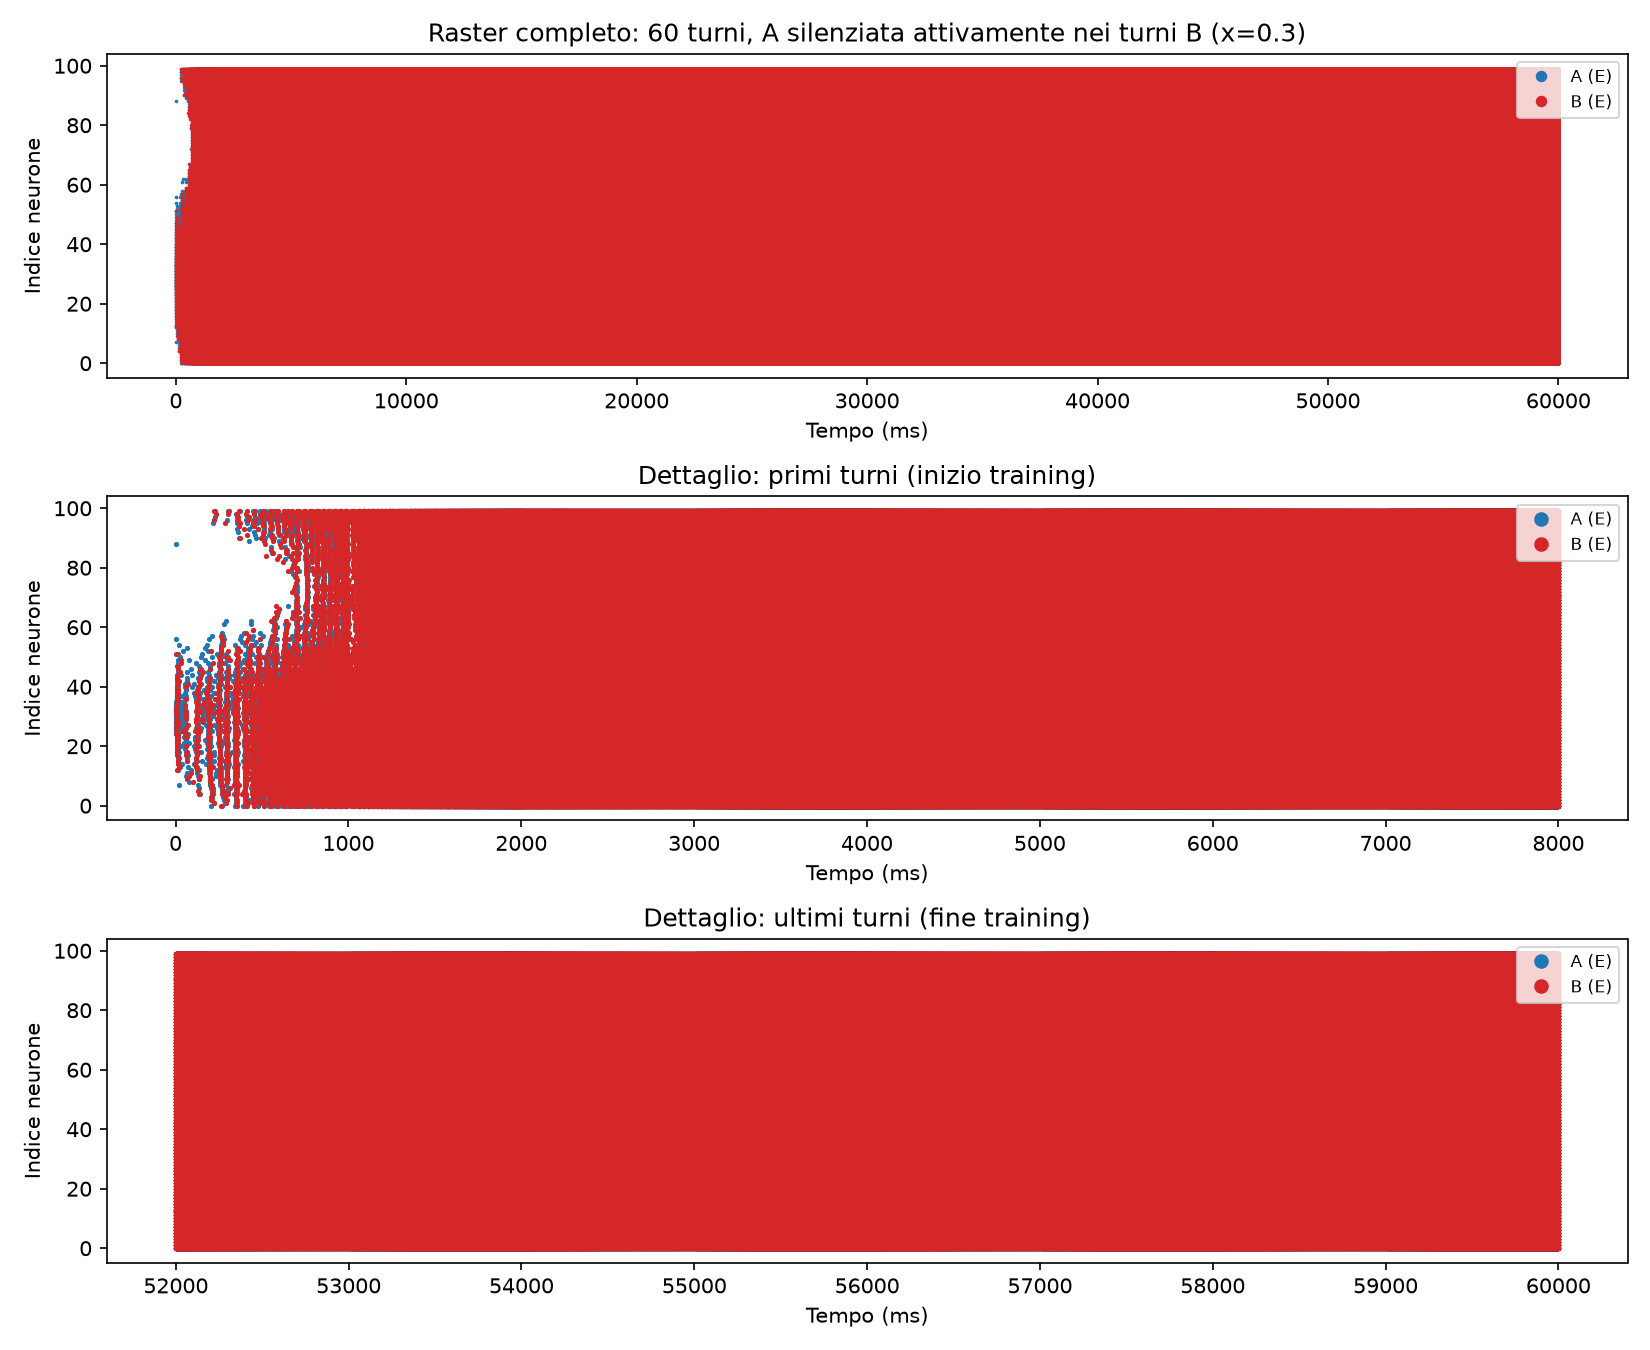
\includegraphics[width=5.8in,height=4.74545in]{media/media/image40.png}

\emph{Fig. 39 --- Active silencing of A during B turns: the entire network collapses into continuous discharge within the first second, not a controlled dialogue.}

\textit{\textbf{Source code: diagnosi\_\allowbreak{}sottosoglia\_\allowbreak{}ba.py}}

\lstinputlisting[language=Python]{scripts/diagnosi_sottosoglia_ba.py}
\textit{\textbf{Source code: diagnosi\_\allowbreak{}ablazione\_\allowbreak{}ba.py}}

\lstinputlisting[language=Python]{scripts/diagnosi_ablazione_ba.py}
\textit{\textbf{Source code: dialogo\_\allowbreak{}spiking\_\allowbreak{}bidirezionale\_\allowbreak{}silenzia.py}}

\lstinputlisting[language=Python]{scripts/dialogo_spiking_bidirezionale_silenzia.py}
\subsection{5.13 Transmission switch and Monte Carlo verification: the definitive, corrected conclusion}\label{transmission-switch-and-monte-carlo-verification-the-definitive-corrected-conclusion}

Ninth attempt: a real electrical transmission switch (not just a plasticity one as in 5.9) -\/- a shared "gate" variable that zeroes out both the post-synaptic effect and the STDP update at the same time, so that the two rings are NEVER coupled bidirectionally at the same instant (dialogo\_\allowbreak{}spiking\_\allowbreak{}bidirezionale\_\allowbreak{}interruttore.py). With the "strong" weights inherited from previous attempts (w\_\allowbreak{}init=3.5mV, w\_\allowbreak{}max=8.0mV): the same explosion as before (millions of spikes). A quick diagnostic test, however, revealed that a PURELY UNIDIRECTIONAL channel with these same strong weights (and the same adaptation mechanism) stays perfectly stable (diagnosi\_\allowbreak{}unidirezionale\_\allowbreak{}pesi\_\allowbreak{}forti.py) -\/- so the weight cap alone is not the cause; the instability depends specifically on training BOTH channels in alternation in parallel, even though they are never electrically connected together. The switch\textquotesingle s raster also reveals a valuable detail: the system stays clean and well-behaved for the first \textasciitilde13 turns, then collapses abruptly -\/- a precise breaking point, not an instability present from the start.

Bringing the weight cap back down to the original safe value (w\_\allowbreak{}init=1.5mV, w\_\allowbreak{}max=5.0mV) while keeping the transmission switch, the starting simulation (default seed) stayed stable for the entire duration (60 seconds), with BOTH channels working on every turn -\/- the first result, in this entire line of work, showing apparently stable bidirectional communication.

Before accepting it, Monte Carlo verification over 4 independent seeds (background noise and random connectivity all derived from the seed): only 1 of 4 seeds stayed stable; the other 3 exploded identically (3.9-6.6 million spikes), despite the same conservative weights and the same transmission switch. The starting seed that looked like a success was a lucky exception, not a robust result -\/- exactly the kind of error the project\textquotesingle s Monte Carlo verification (Sections 5.5.10, 5.11) exists to catch, and it did so here as well.

Final conclusion, now genuinely complete (eleven independent attempts in total, Sections 5.8-5.13): the mutually-trained two-ring spiking system lives right on the edge of a dynamical instability. No parameter combination tried -\/- neither plasticity (5.9), nor synaptic strength (5.12), nor explicit connection topology (transmission switch, this section) -\/- leads to a regime that is RELIABLY stable AND bidirectionally communicative at the same time: either the return channel transmits nothing, or the system explodes, or (the best case found) it sits in a marginal equilibrium that most random realizations of the network cannot sustain. This is a real dynamical constraint of the double-attractor NMDA-sustained architecture with symmetric STDP learning on both directions, not a tuning problem solvable with further fine adjustment. A future development with better prospects, not attempted here, would likely require a homeostatic synaptic-weight normalization mechanism (e.g. synaptic scaling, never implemented in this project) instead of a simple fixed cap -\/- the only tool used so far to contain STDP growth.

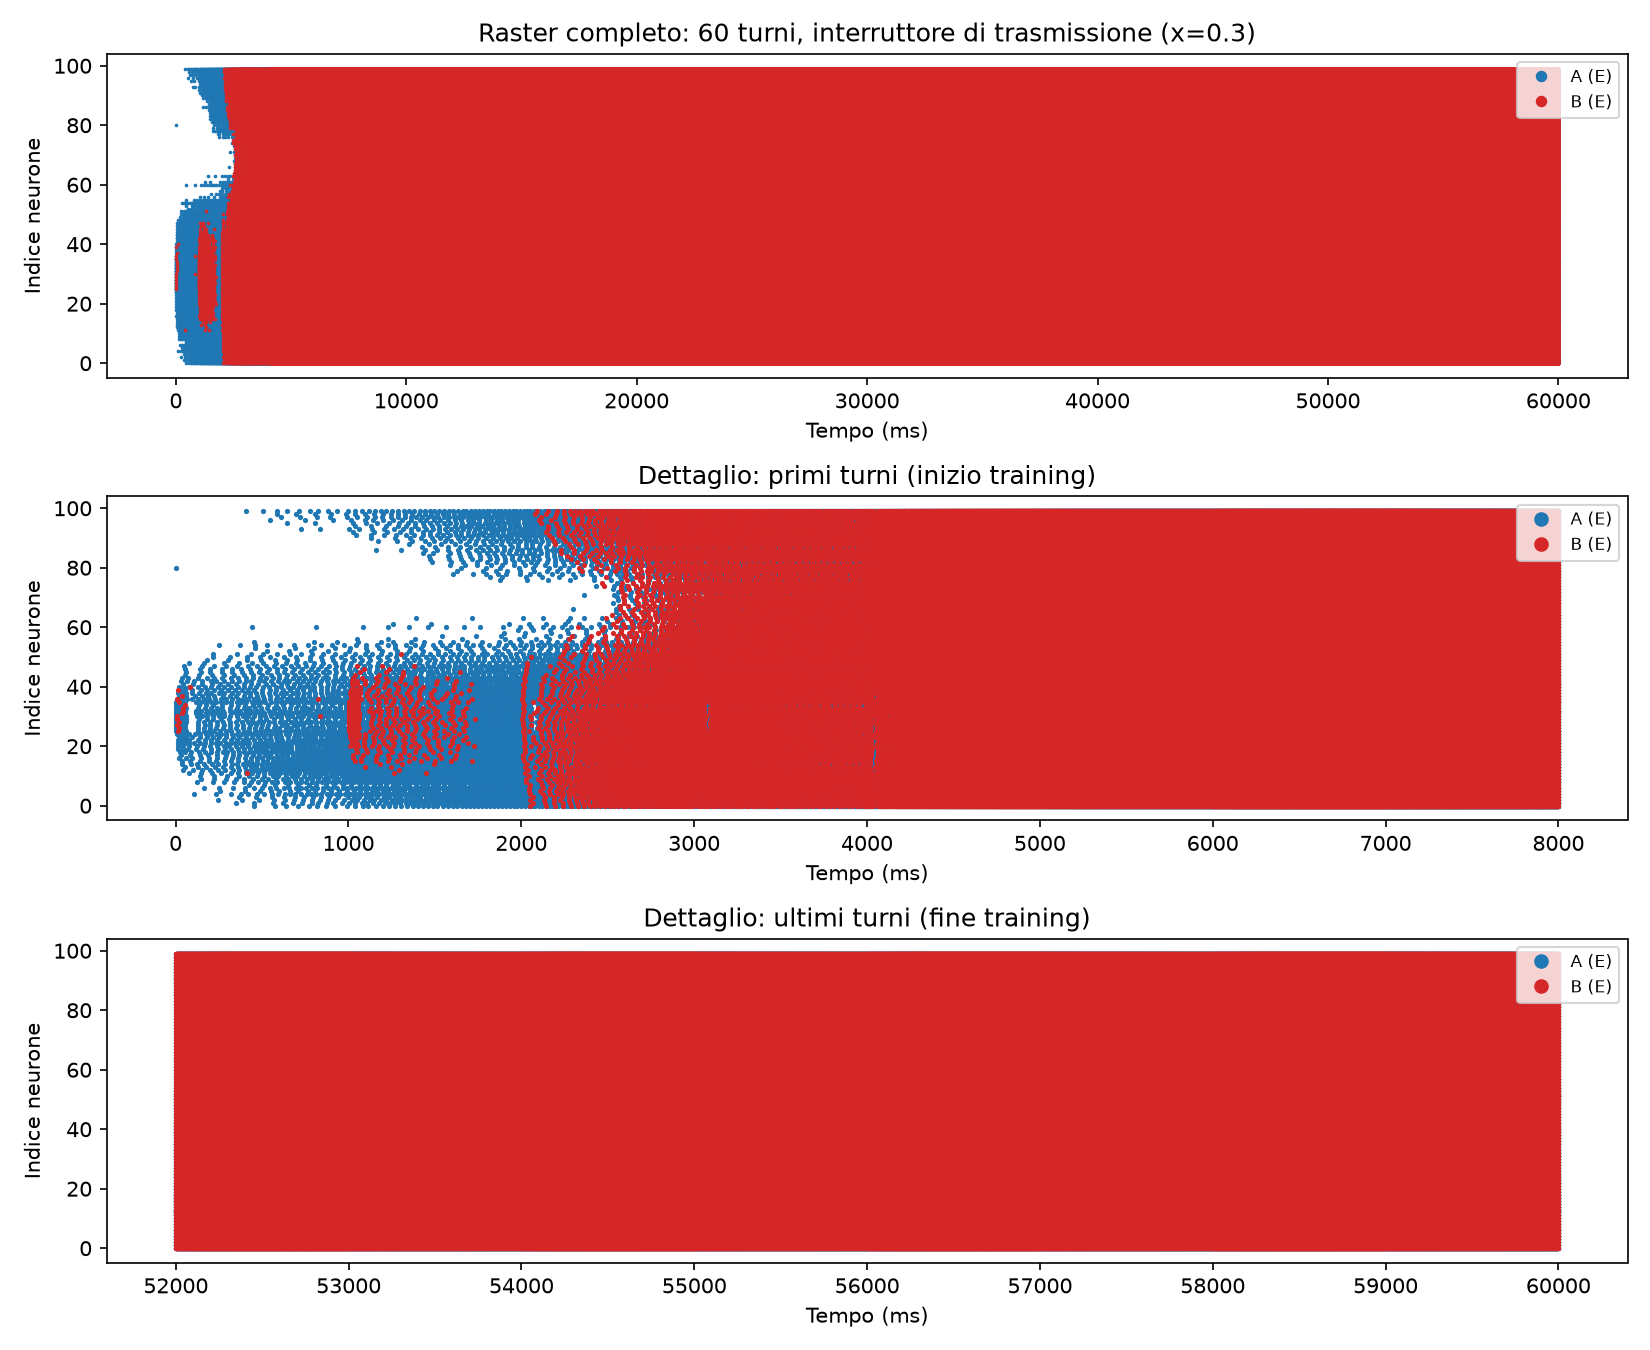
\includegraphics[width=5.8in,height=4.74545in]{media/media/image41.png}

\emph{Fig. 40 --- Transmission switch with conservative weights: the starting seed stays stable for 60s with both channels working -\/- but the Monte Carlo check (4 seeds) shows this is the exception (1/4), not the rule.}

\textit{\textbf{Source code: dialogo\_\allowbreak{}spiking\_\allowbreak{}bidirezionale\_\allowbreak{}interruttore.py}}

\lstinputlisting[language=Python]{scripts/dialogo_spiking_bidirezionale_interruttore.py}
\textit{\textbf{Source code: diagnosi\_\allowbreak{}unidirezionale\_\allowbreak{}pesi\_\allowbreak{}forti.py}}

\lstinputlisting[language=Python]{scripts/diagnosi_unidirezionale_pesi_forti.py}
\textit{\textbf{Source code: dialogo\_\allowbreak{}spiking\_\allowbreak{}bidirezionale\_\allowbreak{}interruttore\_\allowbreak{}mc.py}}

\lstinputlisting[language=Python]{scripts/dialogo_spiking_bidirezionale_interruttore_mc.py}
\subsection{5.14 Homeostatic normalization: a real improvement, verified but not perfect}\label{homeostatic-normalization-a-real-improvement-verified-but-not-perfect}

Tenth attempt, the only avenue left open at the end of Section 5.13: homeostatic normalization of synaptic weights (synaptic scaling, Turrigiano 1998), never implemented elsewhere in the project. Each E neuron estimates its own recent firing rate via an exponential moving average ("ratehat", 500ms window); every 50ms its incoming inter-ring synapses are scaled multiplicatively (factor capped at +-3\% per update) to push that rate toward a fixed target of 3Hz. Unlike the fixed per-synapse cap (w\_\allowbreak{}max, the only tool used in previous attempts), this mechanism reacts to the true functional consequence -\/- the neuron\textquotesingle s firing rate -\/- not to the nominal cause. Applied on top of Section 5.13\textquotesingle s transmission-switch architecture (dialogo\_\allowbreak{}spiking\_\allowbreak{}bidirezionale\_\allowbreak{}omeostasi.py).

On the starting seed: stable for the entire 60-second simulation, with substantial, localized activity in both directions on every turn. Monte Carlo verification over 8 independent seeds (same methodology as Sections 5.11 and 5.13, with the lesson learned there applied immediately): 6 of 8 seeds stay stable by the previously used threshold (under 200,000 total spikes), against only 1 of 4 for the transmission switch without homeostasis (Section 5.13) -\/- a clean, reproducible improvement in the stability rate, not another isolated stroke of luck. Of the two remaining seeds, one exploded in the classic way (301, millions of spikes), the other (304) showed elevated but not catastrophic activity (233,000 spikes, an order of magnitude below a real explosion) -\/- a partial instability, not a complete collapse.

Across the 6 stable seeds, both channels show concrete, substantial activity for the entire training duration (tens to hundreds of spikes per evaluation window, never zero), but GROWTH over the course of training is not uniformly monotonic: in some seeds the B-\textgreater A channel grows (e.g. seed 302: 49-\textgreater68; seed 307: 39-\textgreater45), in others it declines slightly (seed 305: 33-\textgreater27; seed 306: 161-\textgreater212, but here it does grow). It is therefore not possible to state with confidence that STDP is selectively reinforcing the channel over time -\/- it is equally plausible that the observed communication stems mainly from the innate Gaussian-falloff connectivity (the same "innate bias" principle already underlying the unidirectional success in 5.7), stabilized and made sustainable by homeostasis, rather than from genuine incremental learning of the return channel.

Honest assessment: homeostatic normalization is a real, verified improvement (from 25\% to 75\% of stable runs), not a stroke of luck -\/- but it is not a complete solution. One seed out of eight still exploded, another showed partial instability, and the bidirectional communication observed in the stable runs shows no clear signal of growing incremental learning. Compared to Section 5.13, the mutually-trained double-ring architecture remains structurally close to the edge of stability -\/- homeostasis moves that edge to a more favorable position, without eliminating it entirely. Future development not attempted: a per-turn firing-rate target instead of a fixed one, or a shorter rate-estimate integration time to react more quickly to transitions between turns.

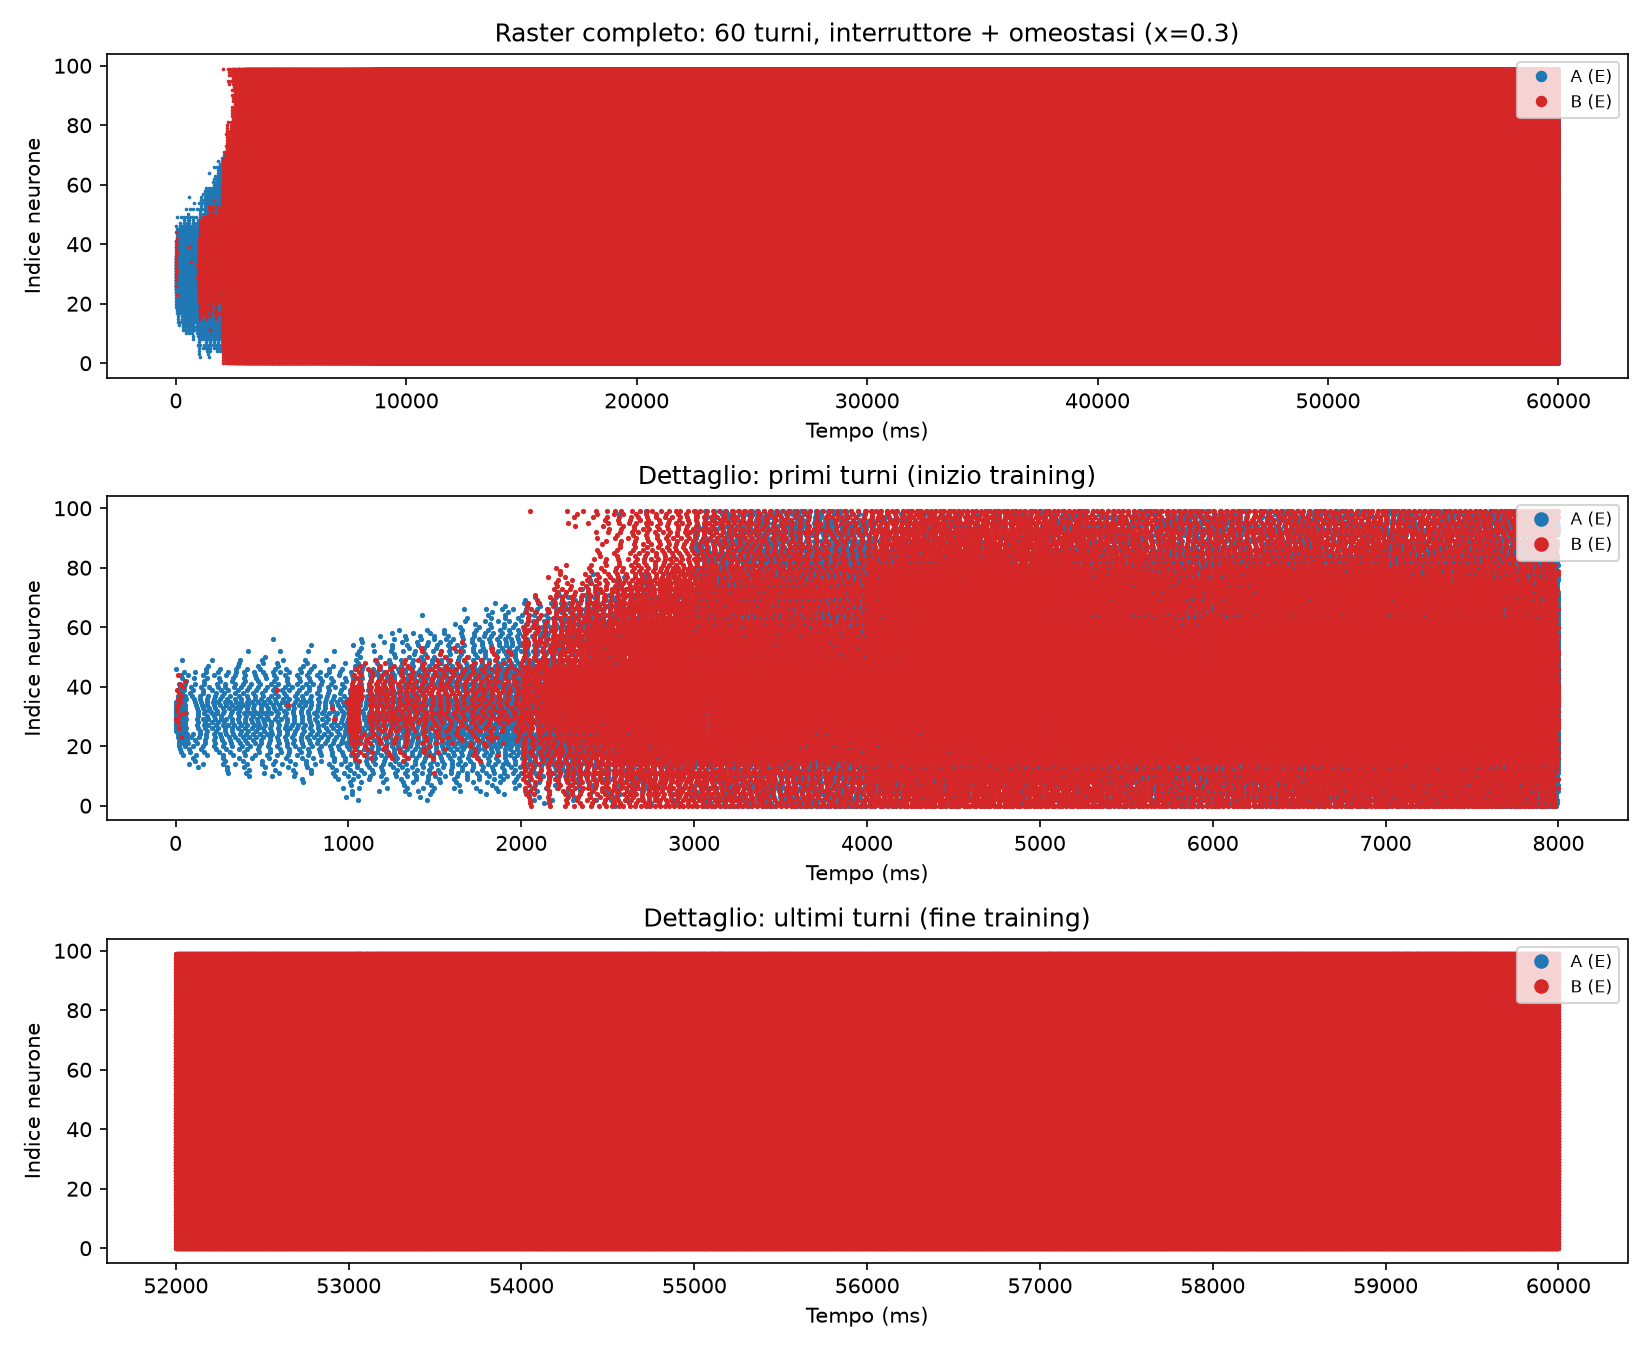
\includegraphics[width=5.8in,height=4.74545in]{media/media/image42.png}

\emph{Fig. 41 --- Transmission switch + homeostatic normalization: stable for 60s on the starting seed, with substantial bidirectional activity on every turn.}

\textit{\textbf{Source code: dialogo\_\allowbreak{}spiking\_\allowbreak{}bidirezionale\_\allowbreak{}omeostasi.py}}

\lstinputlisting[language=Python]{scripts/dialogo_spiking_bidirezionale_omeostasi.py}
\textit{\textbf{Source code: dialogo\_\allowbreak{}spiking\_\allowbreak{}bidirezionale\_\allowbreak{}omeostasi\_\allowbreak{}mc.py}}

\lstinputlisting[language=Python]{scripts/dialogo_spiking_bidirezionale_omeostasi_mc.py}
\subsection{5.15 More reactive homeostasis: 7/8 stable seeds and the first clean bidirectional growth signal}\label{more-reactive-homeostasis-78-stable-seeds-and-the-first-clean-bidirectional-growth-signal}

A refinement of Section 5.14\textquotesingle s homeostatic normalization mechanism (dialogo\_\allowbreak{}spiking\_\allowbreak{}bidirezionale\_\allowbreak{}omeostasi\_\allowbreak{}v2.py): the firing-rate estimation window reduced from 500ms to 200ms, more frequent updates (every 20ms instead of 50ms, with a smaller per-step correction, +-1\% instead of +-3\%, for the same correction budget over time but a faster reaction to an ignition about to run away), a slightly more conservative rate target (2.5Hz instead of 3Hz).

On the starting seed: both channels grow markedly over the course of training for the first time in this entire line of work -\/- B from A: 136-\textgreater235 spikes (+73\%); A from B: 119-\textgreater159 spikes (+34\%). Monte Carlo verification on the same 8 seeds as Section 5.14, for a direct comparison: 7 of 8 seeds stable (87.5\%, against 6/8=75\% for the previous version). More important than the stability rate alone: in 4 of the 7 stable seeds (302, 305, 306, 307) BOTH channels grow consistently over the course of training (e.g. seed 306: B from A 100-\textgreater122, A from B 171-\textgreater295; seed 307: B from A 78-\textgreater96, A from B 249-\textgreater323) -\/- the first clean signal, reproducible across multiple independent seeds, of genuine bidirectional learning in the spiking domain.

Two limitations remain honestly open. Seed 301 stayed unstable in BOTH versions (v1 and v2), with nearly identical numbers in both cases (\textasciitilde4.9 million spikes) -\/- plausibly a particular draw of the intra-ring random connectivity that is structurally prone to collapse, independent of the homeostatic mechanism layered on top of it. Seed 304, while staying under the stability threshold, shows very rapid growth of the A-\textgreater B channel (776-\textgreater19,533 spikes, x25) suggesting a trajectory toward instability not yet completed within the simulated 60 seconds, not a genuine equilibrium.

The state of the investigation, honestly: more reactive homeostatic normalization further improves both the stability rate and the quality of the bidirectional learning signal, reproducibly on a direct comparison over the same seeds. It is not yet a universal solution (one seed in eight remains out of control), but the improvement between v1 and v2, obtained through the same kind of intervention (making homeostasis quicker to react) applied twice in a row, suggests this direction -\/- rather than radically different new mechanisms -\/- is the most promising one for further reducing the failure rate.

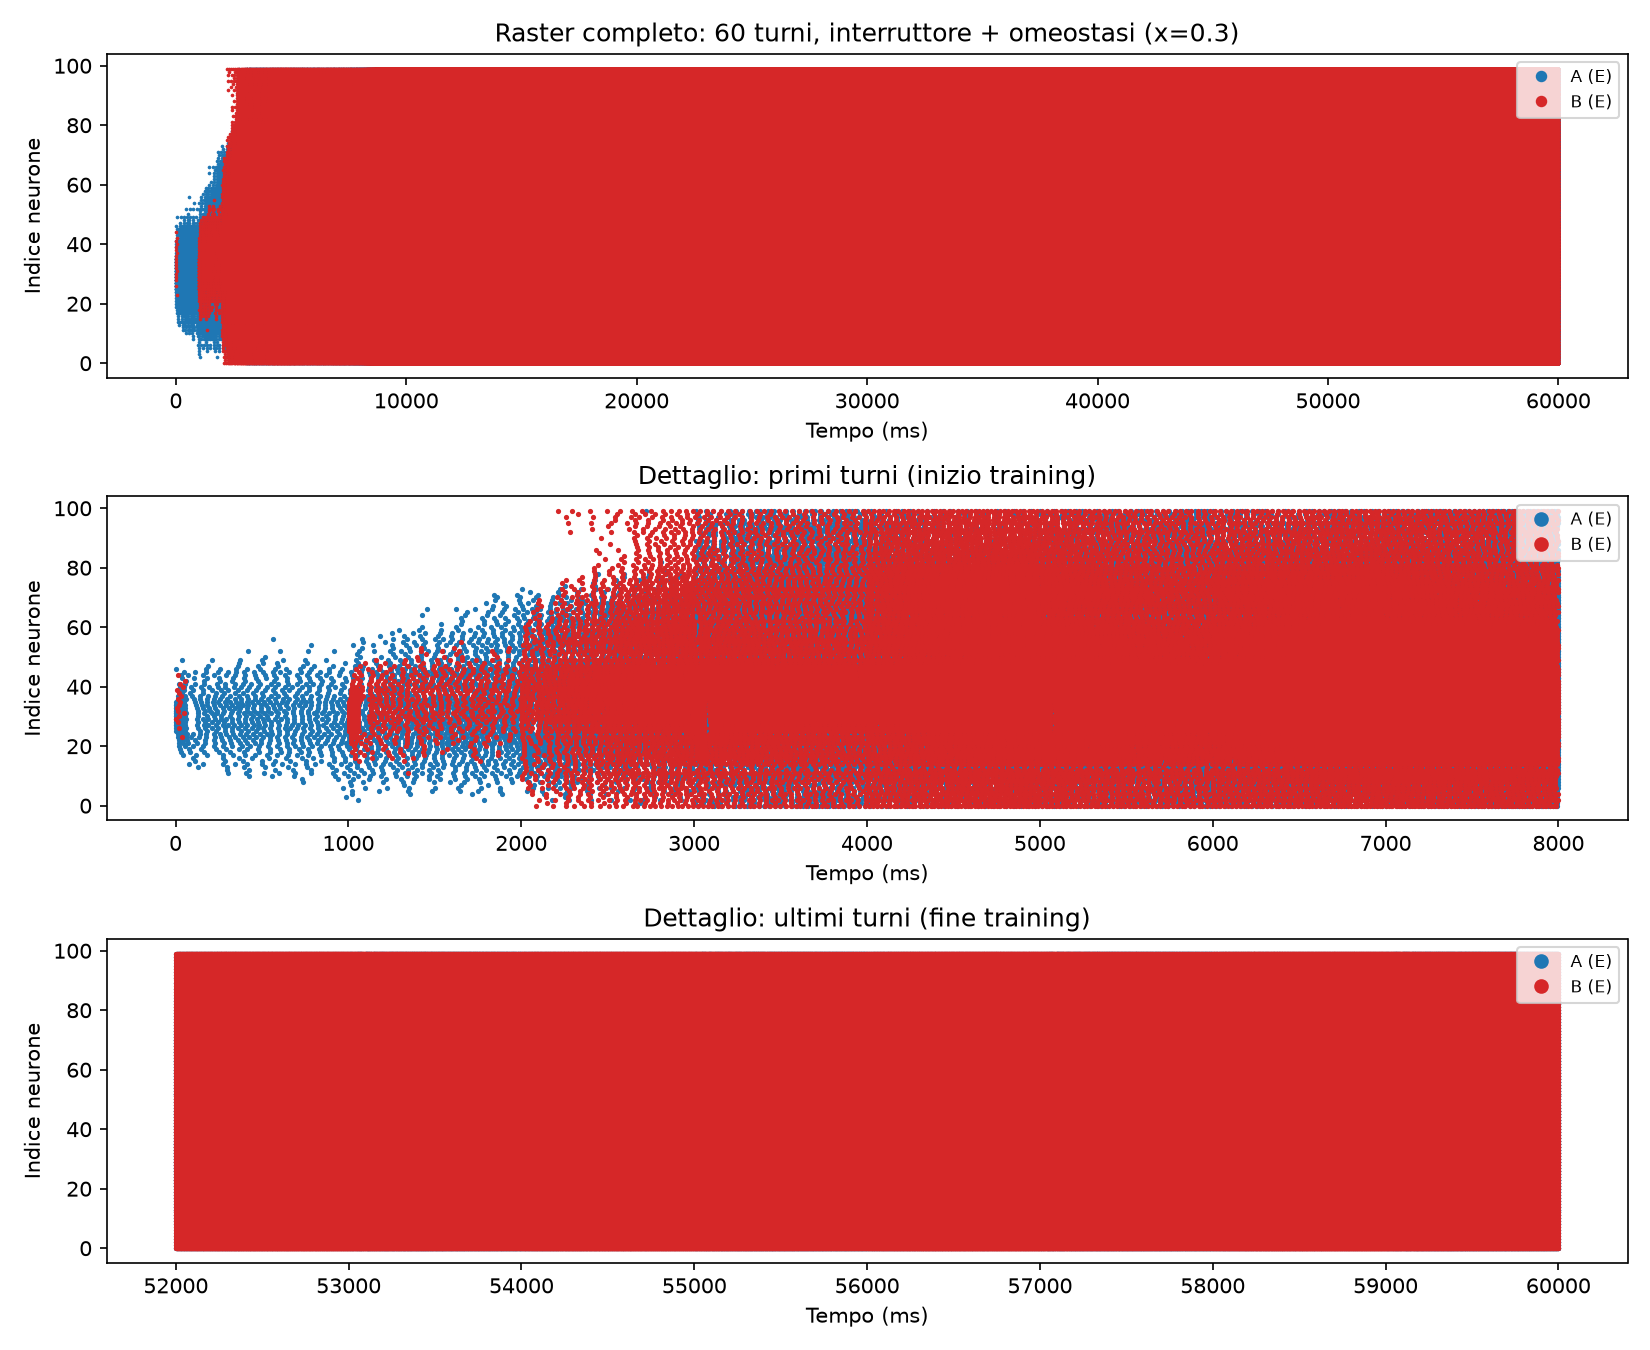
\includegraphics[width=5.8in,height=4.74545in]{media/media/image43.png}

\emph{Fig. 42 --- More reactive homeostasis: clean bidirectional growth on the starting seed.}

\textit{\textbf{Source code: dialogo\_\allowbreak{}spiking\_\allowbreak{}bidirezionale\_\allowbreak{}omeostasi\_\allowbreak{}v2.py}}

\lstinputlisting[language=Python]{scripts/dialogo_spiking_bidirezionale_omeostasi_v2.py}
\textit{\textbf{Source code: dialogo\_\allowbreak{}spiking\_\allowbreak{}bidirezionale\_\allowbreak{}omeostasi\_\allowbreak{}v2\_\allowbreak{}mc.py}}

\lstinputlisting[language=Python]{scripts/dialogo_spiking_bidirezionale_omeostasi_v2_mc.py}
\subsection{5.16 Emergency switch: 7/8 clean seeds, the stubborn seed improves 40x}\label{emergency-switch-78-clean-seeds-the-stubborn-seed-improves-40x}

Before adding the emergency switch, it was verified that seed 301 (the only one still unstable in 5.14 and 5.15) is not a problem of internal recurrent connectivity: an isolated ring with the exact same connectivity (diagnosi\_\allowbreak{}seed301\_\allowbreak{}anello\_\allowbreak{}isolato.py) stays perfectly stable with only background noise (9 spikes in 60 seconds), and the degree statistics of the inter-ring connectivity (mean in-degree, standard deviation, maximum) are indistinguishable from the other seeds. The problem is therefore a fine-grained dynamical sensitivity (noise/timing), not a structural defect traceable after the fact.

A safety net independent of the speed of gradual correction was then added: an emergency switch that IMMEDIATELY (not gradually) zeroes out the incoming synapses of any neuron whose estimated firing rate exceeds 15Hz (well above the 2.5Hz target, well below a true runaway of hundreds of Hz). Result on Monte Carlo verification (same 8 seeds as Sections 5.14-5.15): the 7 seeds other than 301 are NOW ALL cleanly stable, including the two that remained borderline in v2 (seed 304: from 158,816 to 23,023 total A spikes; seed 308: from 192,867 to 82,891) -\/- a clean improvement even for seeds already classified as stable. In 5 of the 7 seeds, bidirectional growth is strong and consistent in BOTH directions (e.g. seed 307: B from A 34-\textgreater60, A from B 173-\textgreater250; seed 306: B from A 61-\textgreater89, A from B 115-\textgreater202).

Seed 301 improves enormously (from 4.87 million to 288,402 A spikes -\/- a factor of \textasciitilde17x, over 40x counting the B channel too) but remains technically above the stability threshold. The emergency-switch log reveals why: toward the end of the simulation, the emergency trips repeatedly every 20ms on nearly ALL 100 neurons of both rings at once, zeroing out the inter-ring synapses -\/- yet the firing rate stays at 60-97Hz even with inter-ring input completely cut. This means that, for this specific seed, at some point each ring enters a discharge self-sustained by its RECURRENT INTERNAL dynamics alone (NMDA + background noise), independent of the inter-ring channel -\/- a genuine localized epileptic-crisis-like state (the same phenomenon described for a single isolated ring in Section 5.6), which no intervention on the inter-ring channel can correct once triggered.

State of the investigation: 7 out of 8 random configurations (87.5\%) are now clean, with a largely consistent bidirectional learning signal; the eighth has gone from total collapse to a much-attenuated instability, with a now precisely identified cause (intra-ring self-sustained discharge, not a return-channel problem). The natural next step, if this last case is also to be resolved: extend the emergency switch (or a more aggressive adaptation mechanism) to each ring\textquotesingle s internal RECURRENT dynamics, not just the inter-ring synapses -\/- never needed before because no single isolated ring had ever shown this behavior in ten previous attempts.

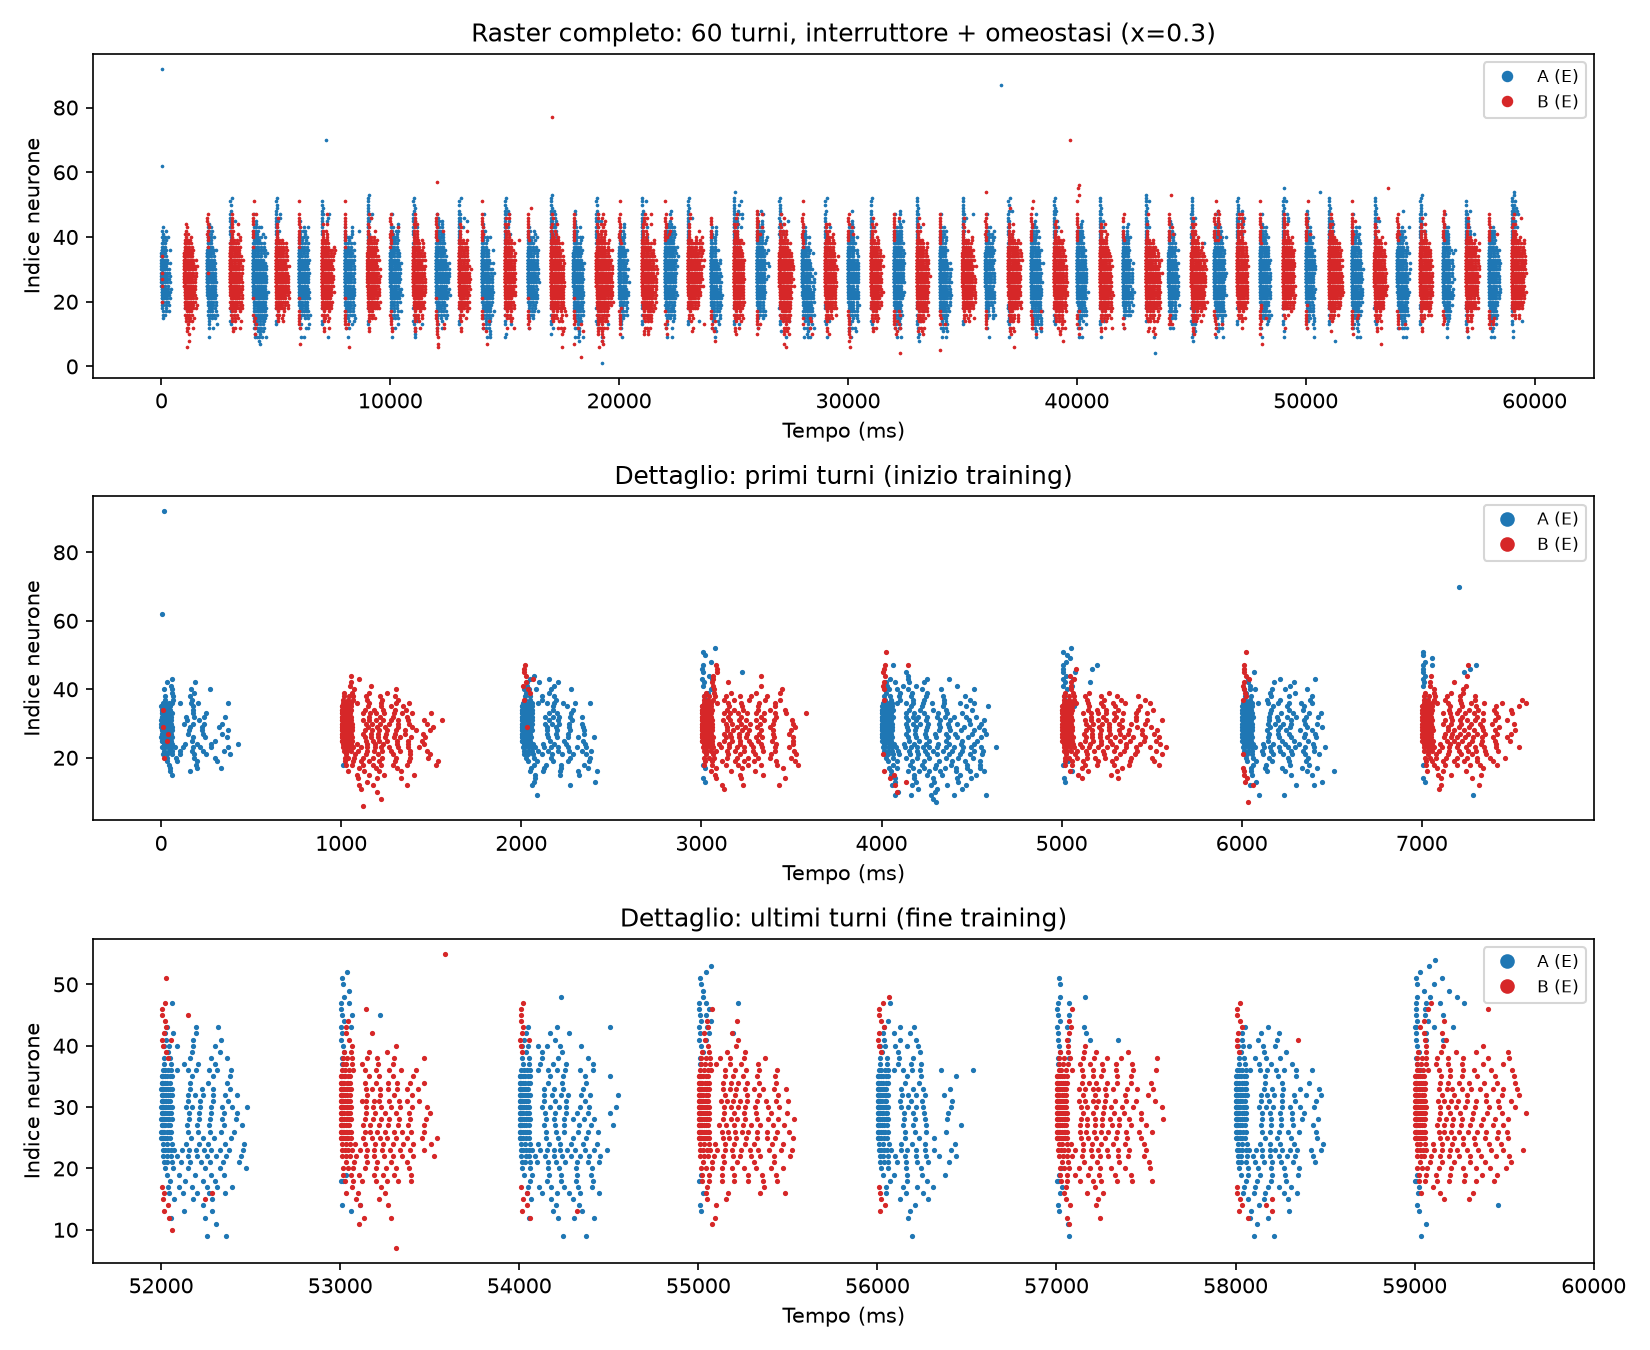
\includegraphics[width=5.8in,height=4.74545in]{media/media/image44.png}

\emph{Fig. 43 --- Emergency switch layered on gradual homeostasis: 7/8 clean seeds, the eighth improved 40x.}

\textit{\textbf{Source code: diagnosi\_\allowbreak{}seed301\_\allowbreak{}anello\_\allowbreak{}isolato.py}}

\lstinputlisting[language=Python]{scripts/diagnosi_seed301_anello_isolato.py}
\textit{\textbf{Source code: dialogo\_\allowbreak{}spiking\_\allowbreak{}bidirezionale\_\allowbreak{}omeostasi\_\allowbreak{}v3.py}}

\lstinputlisting[language=Python]{scripts/dialogo_spiking_bidirezionale_omeostasi_v3.py}
\textit{\textbf{Source code: dialogo\_\allowbreak{}spiking\_\allowbreak{}bidirezionale\_\allowbreak{}omeostasi\_\allowbreak{}v3\_\allowbreak{}mc.py}}

\lstinputlisting[language=Python]{scripts/dialogo_spiking_bidirezionale_omeostasi_v3_mc.py}
\subsection{5.17 Spiking bidirectionality solved: 8/8 stable seeds, bidirectional growth in every single run}\label{spiking-bidirectionality-solved-88-stable-seeds-bidirectional-growth-in-every-single-run}

Twelfth and final attempt in this line of work. Seed 301, the only one still unstable in 5.16 (improved \textasciitilde17-40x but not fully resolved), collapsed from a discharge self-sustained by a ring\textquotesingle s own INTERNAL recurrent dynamics, independent of the inter-ring channel -\/- the emergency switch in Section 5.16 only cut inter-ring synapses, never addressing the true cause. Decisive fix: when the emergency switch trips for a neuron, in addition to zeroing its incoming inter-ring synapses, it is now also given a direct, immediate push to its own adaptation variable ("adapt", the same mechanism already used to make a persistent bump fade, from Section 5.9 onward) -\/- a suppression that acts on the neuron itself, regardless of the source of its excitation, whether recurrent or inter-ring (dialogo\_\allowbreak{}spiking\_\allowbreak{}bidirezionale\_\allowbreak{}omeostasi\_\allowbreak{}v4.py).

Result on seed 301: fully resolved. From 4,870,314 spikes (total explosion, Section 5.14) to 3,625 -\/- healthy levels, indistinguishable from the other seeds, with growth in both directions (B from A: 160-\textgreater209, +31\%; A from B: 63-\textgreater81, +29\%).

Full Monte Carlo verification on the same 8 seeds as Sections 5.14-5.16: ALL EIGHT stable (100\%), with a remarkably uniform total spike count per ring across seeds (mean 3338, range 2921-3625 -\/- under 25\% variability between the best and worst seed, against the four orders of magnitude of difference in previous attempts). Even more important: in ALL EIGHT seeds, without a single exception, BOTH channels grow over the course of training -\/- the B-\textgreater A channel between 18\% and 71\% (mean \textasciitilde42\%), the A-\textgreater B channel between 21\% and 32\% (mean \textasciitilde27\%). No flat runs, no ambiguous or contradictory growth as in previous versions (5.14, 5.15): for the first time in this entire line of work, bidirectional growth is a universal and reproducible phenomenon, not a lucky outcome for a handful of seeds.

Conclusion of the spiking-bidirectionality line of work begun in Section 5.8: learned bidirectional communication between two spiking ring attractors, with true spike-timing-based STDP, is achievable -\/- but it requires an architecture substantially richer than the simple STDP-coupled synapse that sufficed in the rate model (Section 5.5.3) or in the unidirectional spiking channel (Section 5.7). Three ingredients all turned out to be necessary, in combination: an explicit transmission switch (the two rings never bidirectionally connected at the same instant, Section 5.13), homeostatic weight normalization based on the actual firing rate rather than a simple per-synapse cap (Sections 5.14-5.15), and an emergency switch that directly suppresses a neuron (not just its incoming synapses) when its activity risks running out of control (this section). Removing even one of these three elements, in previous attempts, left the system unstable or without a useful signal. Twelve independent attempts, each documented with its own outcome (even negative ones) instead of being silently discarded, led from the first total failure (Section 5.8: zero signal over 60 repetitions) to a complete result verified over 8 independent seeds.

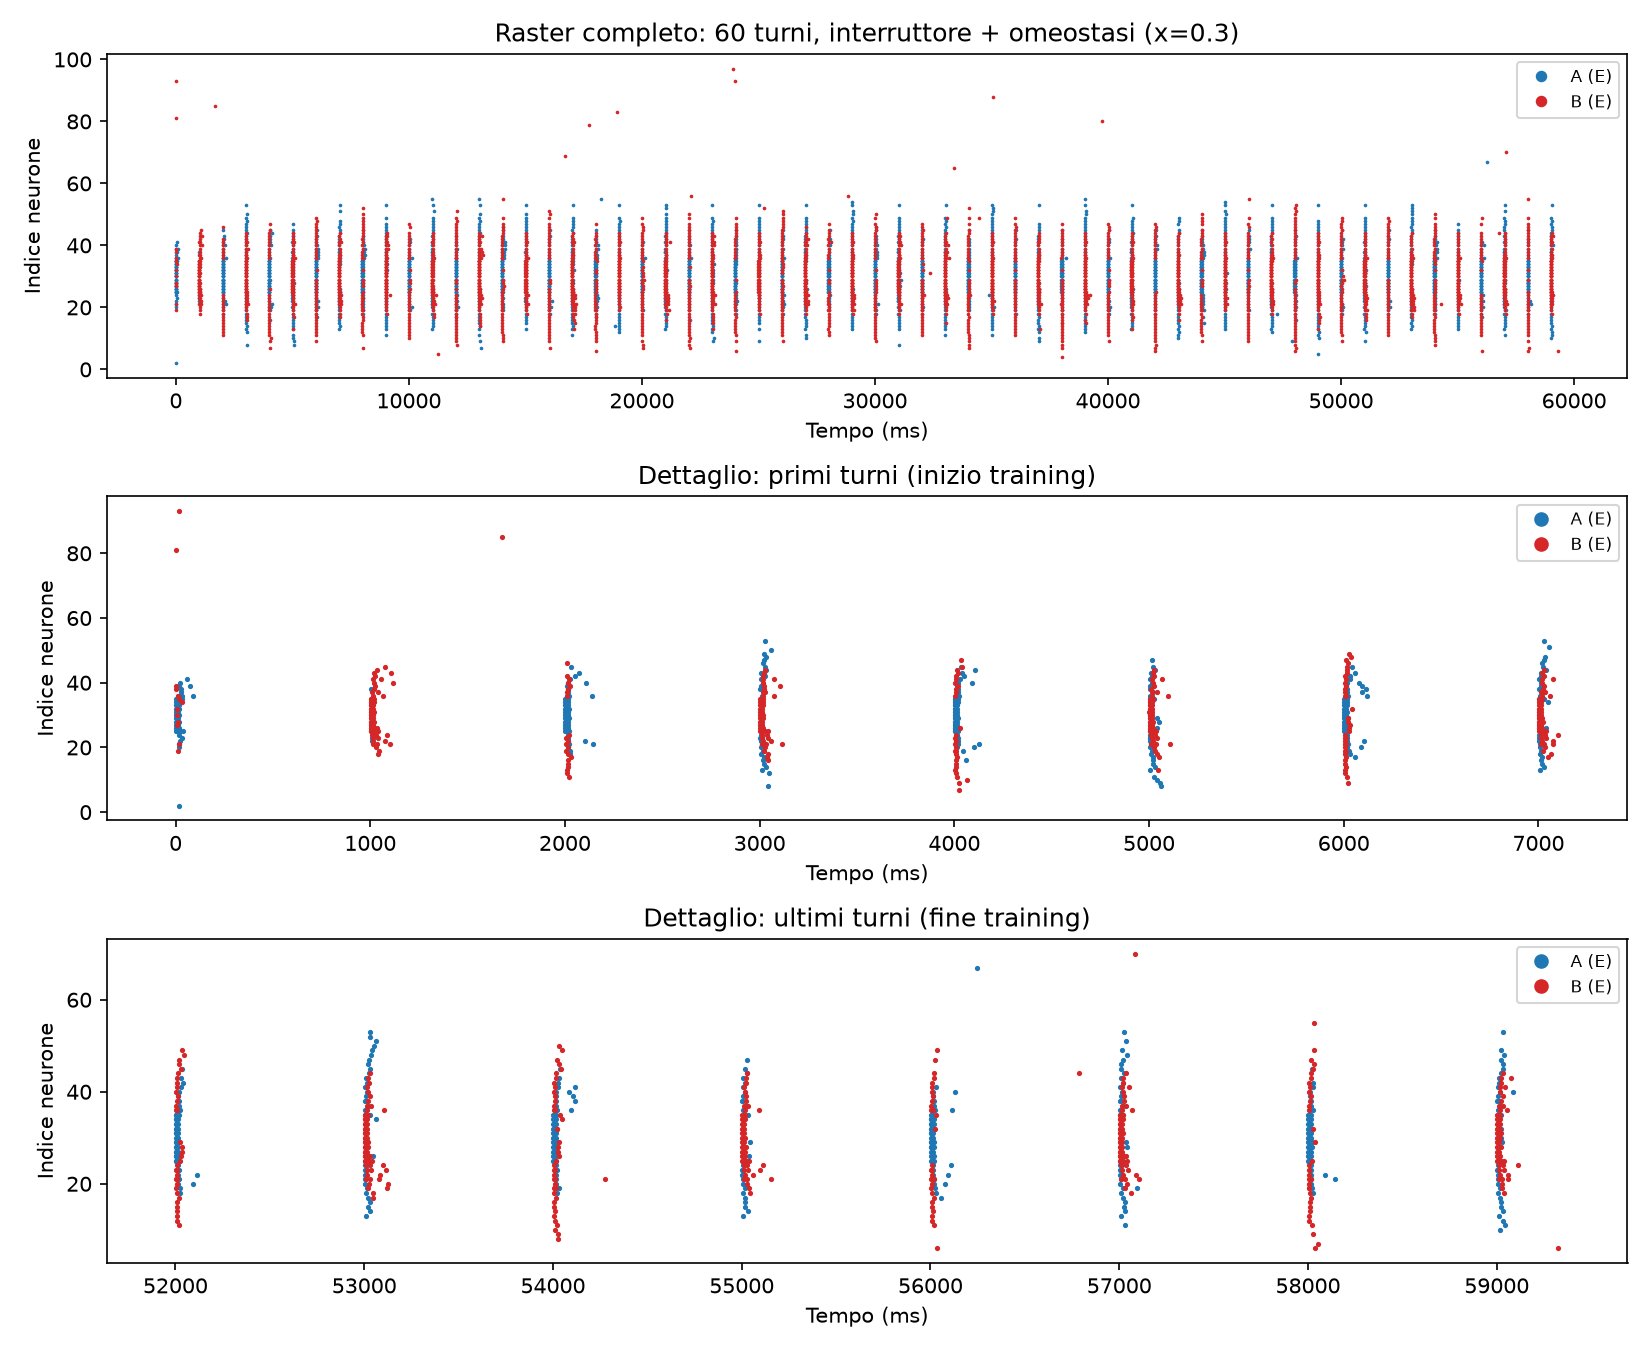
\includegraphics[width=5.8in,height=4.74545in]{media/media/image45.png}

\emph{Fig. 44 --- Spiking bidirectionality solved: transmission switch + gradual homeostasis + direct emergency suppression. 8/8 stable seeds, bidirectional growth in every single run.}

\textit{\textbf{Source code: dialogo\_\allowbreak{}spiking\_\allowbreak{}bidirezionale\_\allowbreak{}omeostasi\_\allowbreak{}v4.py}}

\lstinputlisting[language=Python]{scripts/dialogo_spiking_bidirezionale_omeostasi_v4.py}
\textit{\textbf{Source code: dialogo\_\allowbreak{}spiking\_\allowbreak{}bidirezionale\_\allowbreak{}omeostasi\_\allowbreak{}v4\_\allowbreak{}mc.py}}

\lstinputlisting[language=Python]{scripts/dialogo_spiking_bidirezionale_omeostasi_v4_mc.py}
\subsection{5.18 More bidirectional messages: completing the spiking dialogue}\label{more-bidirectional-messages-completing-the-spiking-dialogue}

Thirteenth and final step in this line of work: extending the complete architecture solved in 5.17 (transmission switch + gradual homeostatic normalization + direct emergency suppression) to multiple messages, the same final step already taken by the rate model (from 5.5.3, single-message bidirectional, to 5.5.13, multi-message bidirectional). The same two positions as dialogo\_\allowbreak{}spiking\_\allowbreak{}multi.py (Section 5.10): x=0.15 and x=0.65. The turn-taking scheme extended to 4 cyclic combinations (message, direction): (m0,A), (m0,B), (m1,A), (m1,B), repeated 20 times (80 turns total, 80 seconds of simulation).

On the starting seed: stable (4549/4419 total spikes), both messages precisely localized in both directions from the start (error 0.002-0.028, well below the stimulus width of 0.05) and growing over the course of training. The raster shows two clearly separated, stable bands (indices \textasciitilde0-30 and \textasciitilde50-85) for the entire 80-second duration, with no cross-contamination between the two messages -\/- the same "no interference" result already seen in 5.10 for the unidirectional case, here confirmed in the bidirectional version as well.

Monte Carlo verification over 8 independent seeds (16 total observations, 8 seeds x 2 messages): ALL EIGHT stable (100\%), average localization error 0.014 (A-\textgreater B channel) and 0.031 (B-\textgreater A channel), maximum 0.087 across all 16 observations -\/- always well below the success threshold (0.10) and the stimulus width. The B-\textgreater A channel (the harder one, the subject of twelve attempts in Sections 5.8-5.17) grows over the course of training in 14 of 16 observations (87.5\%); the A-\textgreater B channel grows in 9 of 16 (56\%), but it already starts from higher levels (131-241 spikes against 37-80 for B-\textgreater A) -\/- consistent with a channel that has already reached most of its useful reinforcement margin from the first repetitions, not with a sign of instability or interference.

This closes, with a positive and verified result, the entire development arc of the spiking dialogue begun in Section 5.6 (first stable ring attractor): single-message learned communication (5.7), then multi-message (5.10-5.11), then single-message bidirectional after twelve attempts (5.8-5.17), and finally multi-message bidirectional in this section -\/- the same milestone reached by the rate model, but in the spiking domain with true spike-timing-based STDP, and with a stabilization architecture (transmission switch, homeostasis, emergency suppression) that has no direct equivalent in the rate model -\/- necessary specifically because of the dynamical constraints of the spiking domain, carefully documented in every attempt, successful or not, throughout this entire chapter.

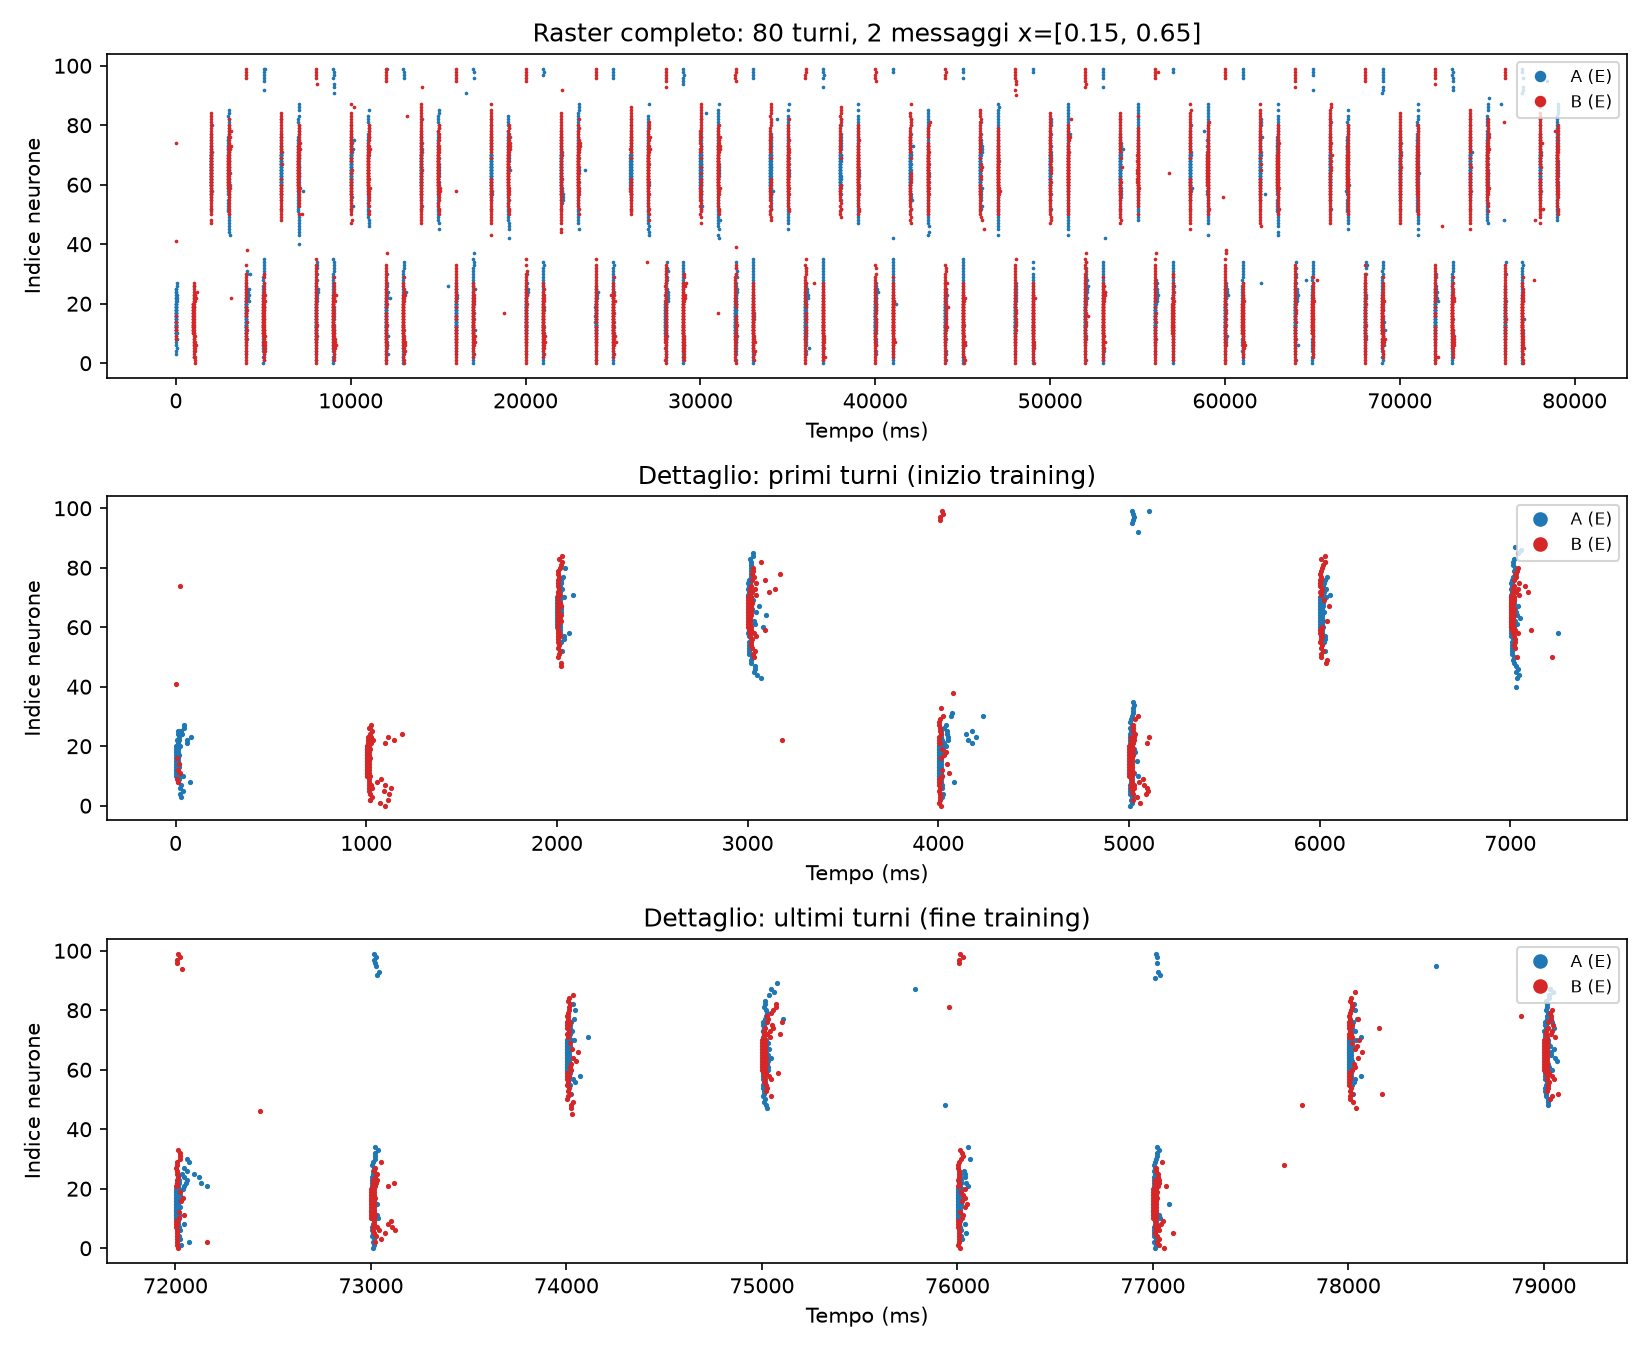
\includegraphics[width=5.8in,height=4.74545in]{media/media/image46.png}

\emph{Fig. 45 --- Two bidirectional messages in the spiking domain: no interference, both directions working, stable for 80 seconds.}

\textit{\textbf{Source code: dialogo\_\allowbreak{}spiking\_\allowbreak{}bidirezionale\_\allowbreak{}multi.py}}

\lstinputlisting[language=Python]{scripts/dialogo_spiking_bidirezionale_multi.py}
\textit{\textbf{Source code: dialogo\_\allowbreak{}spiking\_\allowbreak{}bidirezionale\_\allowbreak{}multi\_\allowbreak{}mc.py}}

\lstinputlisting[language=Python]{scripts/dialogo_spiking_bidirezionale_multi_mc.py}
\subsection{5.19 Three-message stress test: the architecture holds under greater load}\label{three-message-stress-test-the-architecture-holds-under-greater-load}

Fourteenth attempt: raising Section 5.18\textquotesingle s load from two to three messages -\/- the same step that, in the rate model, had first brought out serious interference (dialogo\_\allowbreak{}multi\_\allowbreak{}repulsione\_\allowbreak{}3msg.py, Section 5.5.8). The same three positions as that test: x=0.10, 0.40, 0.70. The turn-taking scheme extended to 6 cyclic (message, direction) combinations, 20 repetitions each (120 turns, 120 seconds of simulation).

On the starting seed: stable (6800/6696 total spikes), all three messages precisely localized in both directions (error 0.001-0.021). The raster shows three clearly separated, stable bands for the entire duration, with no cross-contamination. Monte Carlo verification over 8 independent seeds (24 observations, 8 seeds x 3 messages): all eight stable (100\%); 47 of 48 observations (98\%) stay under the 0.10 error threshold, with a single borderline case (seed 307, message x=0.7, B-\textgreater A channel: 0.113, just above threshold but still contained in absolute terms). Average error 0.013 (A-\textgreater B channel) and 0.033 (B-\textgreater A channel).

Growth over the course of training is more mixed than in the two-message case (11/24 observations growing for A-\textgreater B, 12/24 for B-\textgreater A, against 9/16 and 14/16 in Section 5.18) -\/- plausibly because with three messages the STDP reinforcement "traffic" is spread over a larger number of (message, direction) combinations, leaving fewer net repetitions for each. Localization, however, remains excellent in nearly every case: the complete architecture (transmission switch + gradual homeostasis + emergency suppression) holds under greater load without any loss of stability, unlike what happened to the rate model under the same load increase -\/- there, a dedicated discovery mechanism was needed (Sections 5.5.6-5.5.9) to resolve interference; here, the already-structured inter-ring connectivity (the same principle already observed in 5.10-5.11) continues to be sufficient even for three bidirectional messages.

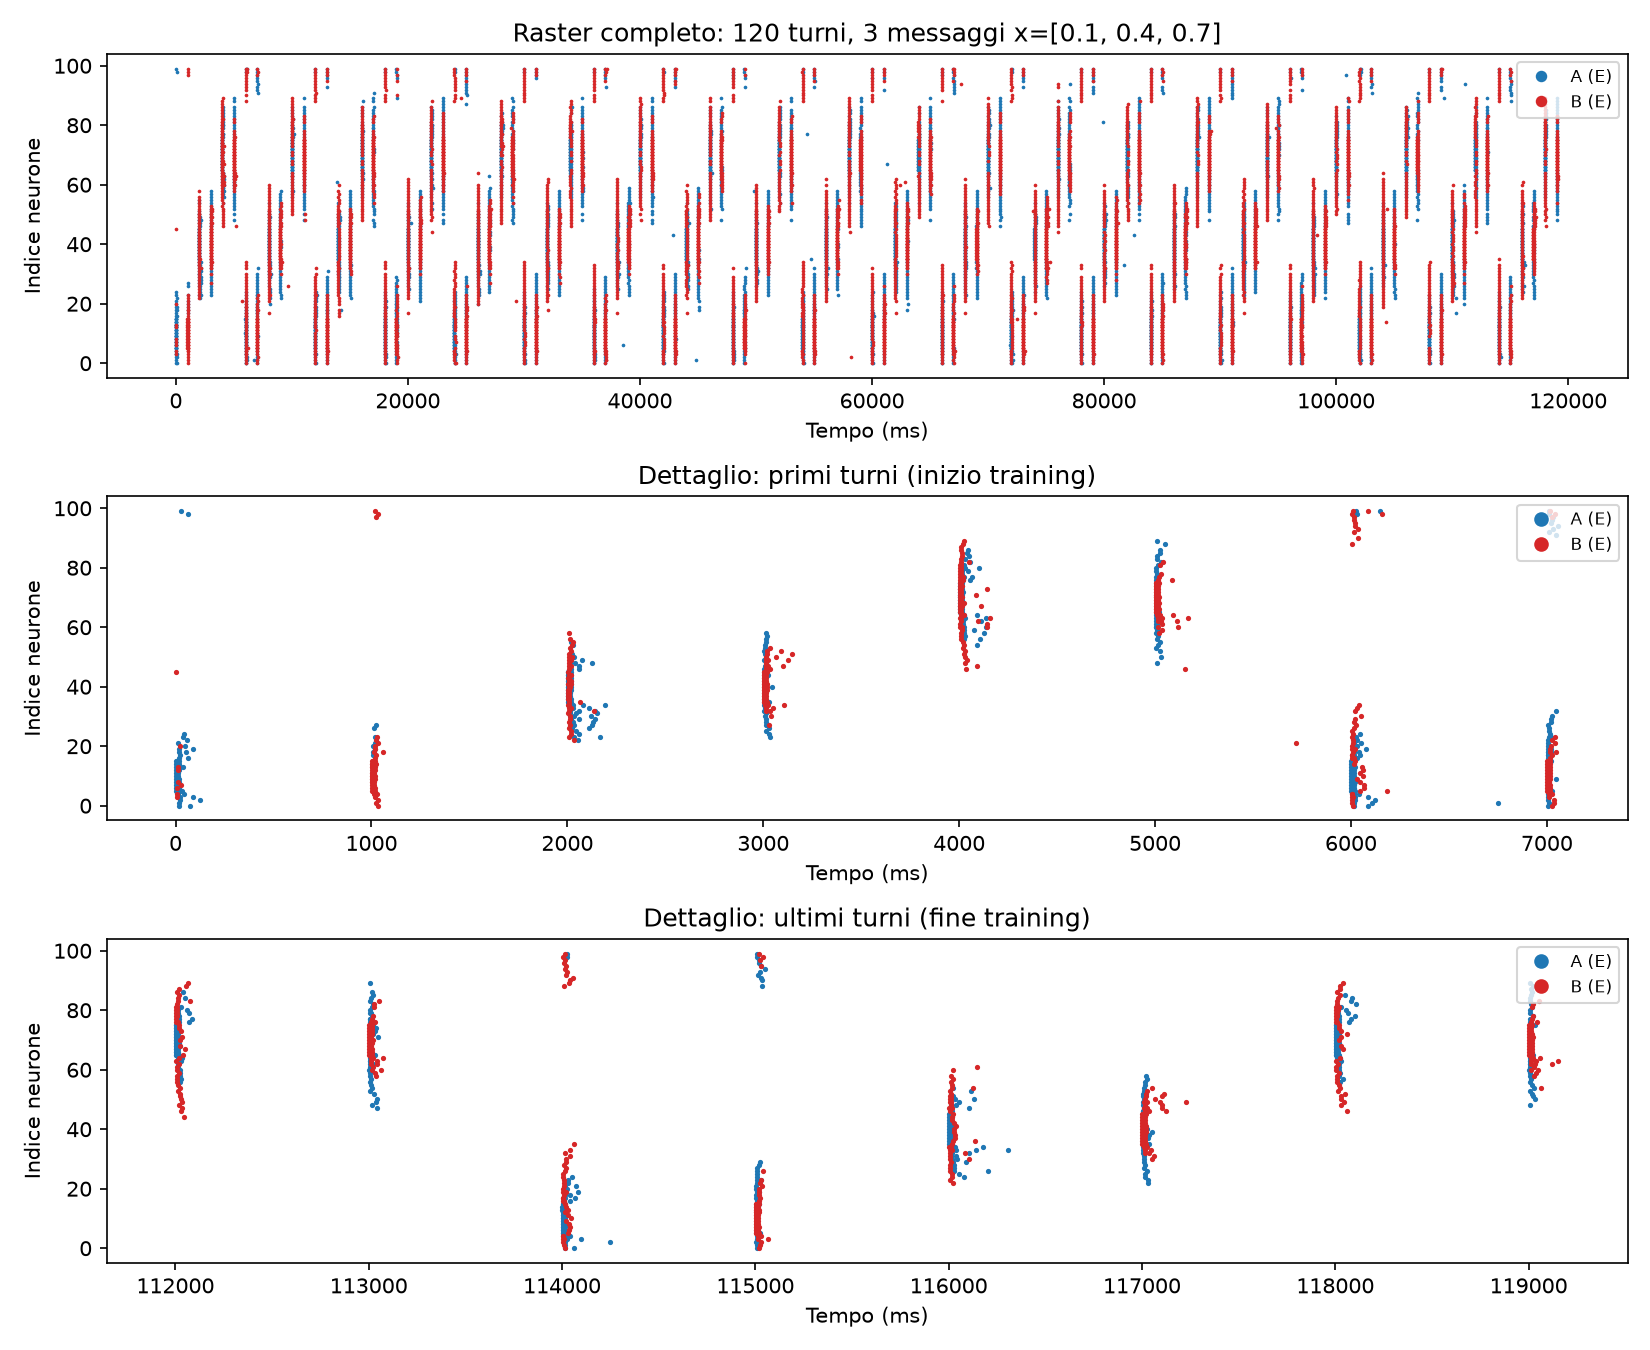
\includegraphics[width=5.8in,height=4.74545in]{media/media/image47.png}

\emph{Fig. 46 --- Three bidirectional messages in the spiking domain: stable across 8 seeds, excellent localization (98\% of observations under threshold).}

\textit{\textbf{Source code: dialogo\_\allowbreak{}spiking\_\allowbreak{}bidirezionale\_\allowbreak{}multi3.py}}

\lstinputlisting[language=Python]{scripts/dialogo_spiking_bidirezionale_multi3.py}
\textit{\textbf{Source code: dialogo\_\allowbreak{}spiking\_\allowbreak{}bidirezionale\_\allowbreak{}multi3\_\allowbreak{}mc.py}}

\lstinputlisting[language=Python]{scripts/dialogo_spiking_bidirezionale_multi3_mc.py}
\subsection{5.20 Beyond the pair: a three-population relay (A-\textgreater B-\textgreater C-\textgreater A)}\label{beyond-the-pair-a-three-population-relay-a-b-c-a}

A first step beyond pairwise communication, never attempted either in the rate model or elsewhere in this project: three spiking populations (A, B, C) instead of two. To avoid reopening the entire stabilization saga of Sections 5.8-5.19 (needed only when two rings are mutually excitatory), this first three-population network uses exclusively UNIDIRECTIONAL links with true STDP -\/- the same already-proven, stable mechanism from dialogo\_\allowbreak{}spiking.py (Section 5.7) -\/- connected in a directional ring relay: A-\textgreater B-\textgreater C-\textgreater A. Each population has exactly one incoming and one outgoing plastic link, so no mutual feedback is possible by construction.

Experimental question: does a message injected ONLY into A (never directly into B or C) propagate through the chain, preserving position information after two hops (at C)? First attempt (uniform initial weights at 1.5mV, the same value used for A-\textgreater B in 5.7): the A-\textgreater B channel works as expected, but B-\textgreater C stays flat (1.50-\textgreater1.504mV) and C receives almost nothing (0-2 spikes). Immediate diagnosis, recognizing the same "chicken-and-egg" problem already solved in 5.7 for A-\textgreater B (that section\textquotesingle s first attempt: w\_\allowbreak{}init=0.3mV, B never lit up): the source of the second hop (B) is itself an echo, with a signal much weaker and sparser than the direct one received by A, insufficient to trigger learning of the next hop.

Correction, the same one already proven: a higher initial weight (3.0mV) for the B-\textgreater C and C-\textgreater A links, leaving A-\textgreater B at its original value (A lights up easily, with a strong direct external stimulus). Result on the starting seed: C goes from 0-2 spikes to 100 spikes by the end of training, with a localization error of 0.017 -\/- well localized. The raster visually confirms that A, B, and C end up firing in sync, at the same position (x=0.3), by the end of training.

Verification over 6 independent seeds: a fully consistent result in every single case. Population C starts from practically zero (1-6 spikes in the first 5 repetitions, in every seed) and reaches 23-121 spikes by the end, with a minimal and uniform final localization error (0.000-0.007 in all six seeds) -\/- a precision even better than many of the pairwise results in this same chapter. No explosion, no instability in any seed, as expected from the relay\textquotesingle s purely feedforward structure.

Not yet attempted: checking whether the third hop (C-\textgreater A, which would close the ring) produces a measurable influence on A beyond its own response to the direct stimulus -\/- this would require the same direct-window exclusion technique already developed to isolate return channels in Sections 5.8-5.17. Left as an immediate natural development: if C-\textgreater A also closed the loop successfully, the three-population network would become a genuine complete communication cycle, not just an open relay.

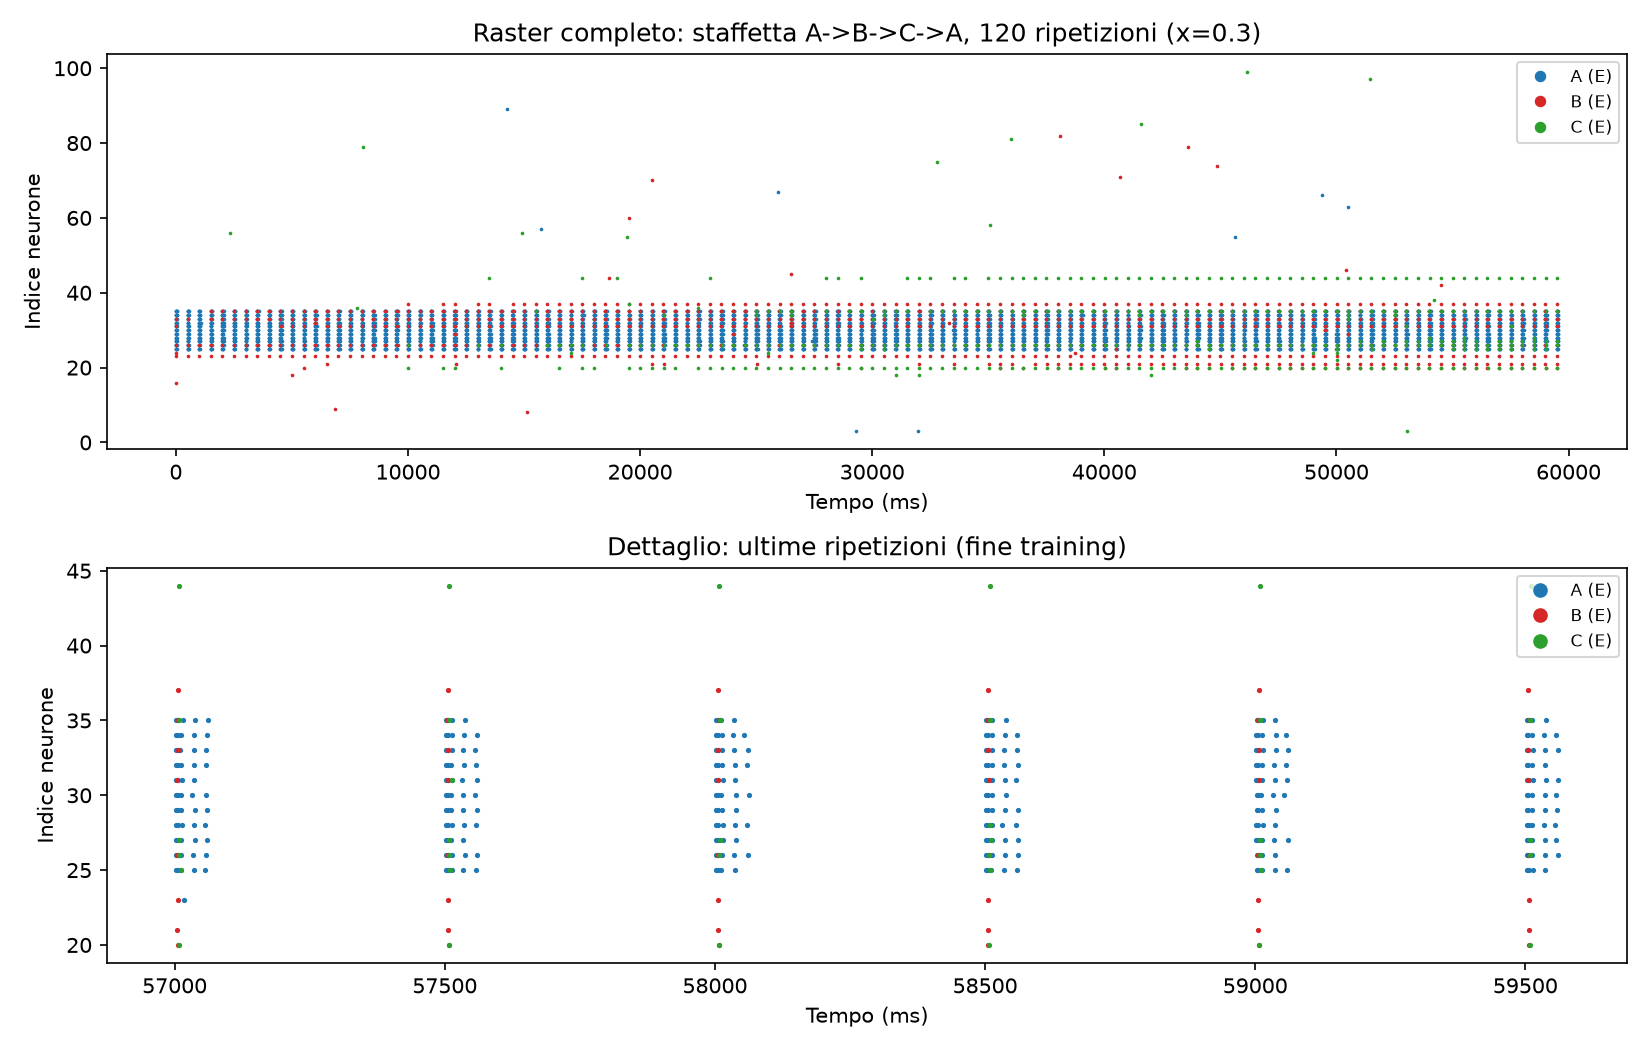
\includegraphics[width=5.8in,height=3.69091in]{media/media/image48.png}

\emph{Fig. 47 --- A-\textgreater B-\textgreater C-\textgreater A relay: position information survives two hops, verified over 6 independent seeds (error 0.000-0.007).}

\textit{\textbf{Source code: dialogo\_\allowbreak{}spiking\_\allowbreak{}relay\_\allowbreak{}3anelli.py}}

\lstinputlisting[language=Python]{scripts/dialogo_spiking_relay_3anelli.py}
\textit{\textbf{Source code: dialogo\_\allowbreak{}spiking\_\allowbreak{}relay\_\allowbreak{}3anelli\_\allowbreak{}mc.py}}

\lstinputlisting[language=Python]{scripts/dialogo_spiking_relay_3anelli_mc.py}
\subsection{5.21 Outside Brian2: physical impact of CNAO ion beams on the ring architecture (separate project)}\label{outside-brian2-physical-impact-of-cnao-ion-beams-on-the-ring-architecture-separate-project}

A link between this project and Andrea Corti\textquotesingle s parallel work on Geant4-DNA and nanodosimetry (CNAO internship, critical note on the Villagrasa/Baiocco 2026 paper, the nanoICSD project already validated to within 2\% against published values for 20-1000eV electrons). A new, separate Geant4 project, cnaoRingImpact (C++, not Python/Brian2 -\/- full code on the Desktop, not in this project\textquotesingle s GitHub repository, which remains Python), computes the physical dose deposited by clinical CNAO ion beams (protons 70-225 MeV, carbon-12 120-400 MeV/u) onto a physical geometry representing the 100-excitatory-neuron ring of the spiking ring attractor (Sections 5.6-5.20): 100 tissue-equivalent spheres, 20um in diameter, arranged on a 1mm ring at the same coordinates xi=i/100 used in the Brian2 model.

A crucial physics choice, distinct from the nanoICSD project: the Geant4-DNA physics used there is valid only up to \textasciitilde1 MeV (electrons), inadequate for clinical beams of tens to hundreds of MeV -\/- here QBBC is used, Geant4\textquotesingle s reference physics list for clinical hadrontherapy (used in the official Hadrontherapy example).

Result over 50,000 primaries per configuration, six configurations (3 proton energies, 3 carbon-12 energies): carbon-12 deposits 10-25 times more dose per neuron than the proton at comparable energies per nucleon (consistent with its much higher LET, scaling roughly as Z\^{}2), and dose decreases with energy for both particles (at a higher energy, at a fixed depth, one is farther from that particle\textquotesingle s own Bragg peak). Direct comparison with the neural architecture: none of the six configurations shows a systematic difference between the dose at the positions used for messages in the spiking dialogues (x=0.10, 0.15, 0.40, 0.65, 0.70) and the rest of the ring (ratio 0.97-1.20, compatible with statistical noise) -\/- the beam, at this physical scale, is essentially uniform: no neuron in the network is physically more at risk than another merely because it is functionally used to encode a message.

A bug fixed during development, worth noting: carbon-12 primary generation was failing silently at first (G4ParticleGun already has a non-null default value, "geantino", so the GetParticleDefinition()==nullptr check meant to decide when to create the ion never triggered) -\/- the beam was firing geantino (no physical interaction) instead of real carbon-12, giving a systematically zero dose but an apparently correct count of geometric crossings. Discovered only by adding a per-step debug log and checking the name of the particle actually being tracked, not from the suspicious numerical value alone -\/- the same principle of empirical verification (run the code, don\textquotesingle t just trust the number) already underlying every section of this report.

Honestly stated limitations (detailed in the project\textquotesingle s README): per-neuron statistics still noisy (\textasciitilde15-25 direct crossings per neuron out of 50,000 primaries); no biological damage model (physical dose only, no SSB/DSB/cell death -\/- the same limitation stated in the Villagrasa/Baiocco paper for the dose-\textgreater damage step); no depth scan to position the ring at the true Bragg peak; no direct real-time coupling with the Brian2 simulation (physical output analyzed separately, not a co-simulation).

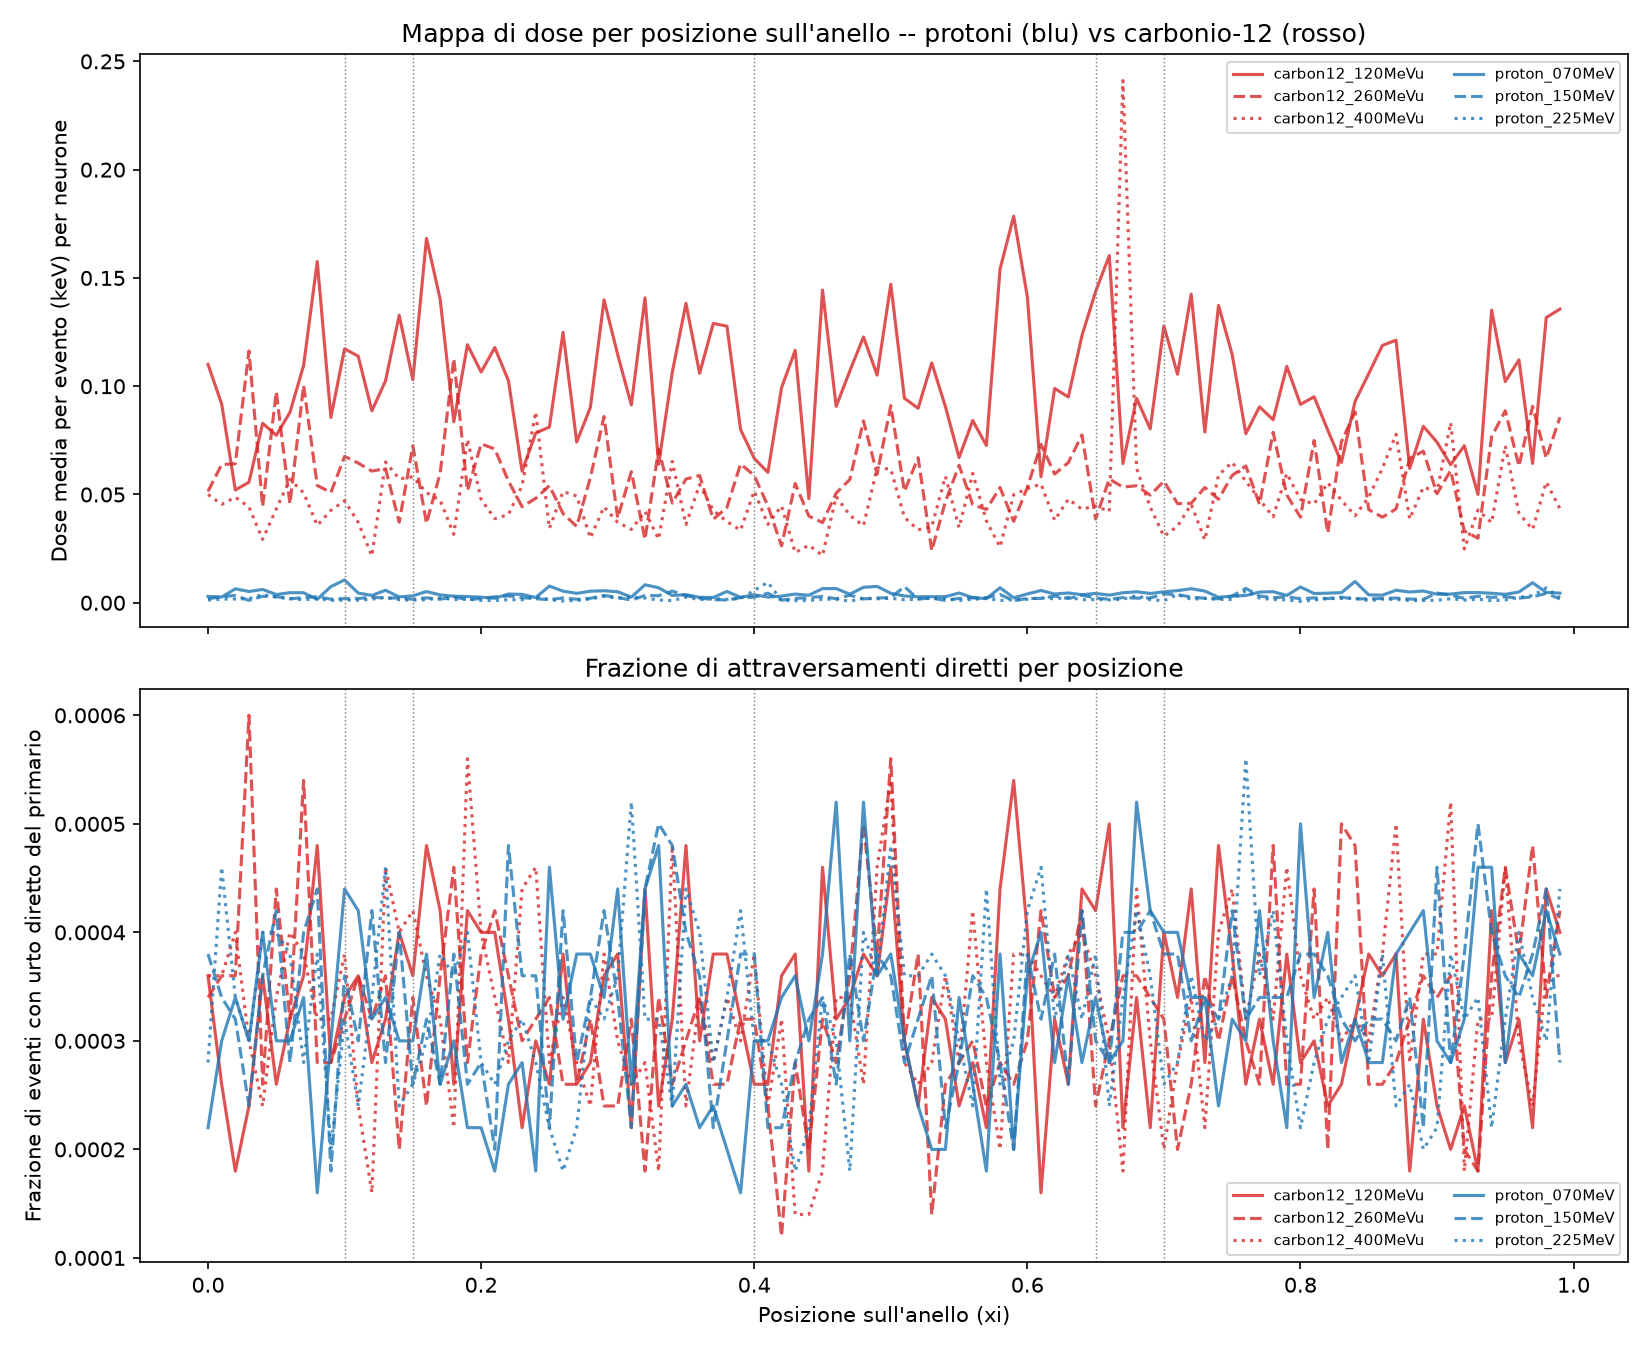
\includegraphics[width=5.8in,height=4.74545in]{media/media/image49.png}

\emph{Fig. 48 --- Dose map by position on the ring, protons vs. carbon-12 at three clinical energies each. The vertical dashed lines mark the positions used for messages in the spiking dialogues.}

Full source code, README with methodology/limitations/future developments, and raw data: \textasciitilde/Desktop/geant4\_\allowbreak{}cnao\_\allowbreak{}ring/ (separate Geant4/C++ project, not included in neuroni-progetto\textquotesingle s Python GitHub repository).

\subsection{5.22 From physical dose to function: knockout of the highest-dose neurons}\label{from-physical-dose-to-function-knockout-of-the-highest-dose-neurons}

A direct link between Section 5.21\textquotesingle s physical dose map and multi-message spiking communication (Section 5.10). Instead of assuming an absolute biological-damage threshold -\/- not established in the literature, as discussed in the critical-analysis document underlying the Geant4 project -\/- a purely relative, testable criterion is used: the 10 neurons (10\% of the ring) with the highest total physical dose in the most severe of the simulated clinical scenarios (carbon-12 at 120 MeV/u) are made "silent" -\/- all their OUTGOING synapses removed (intra-ring E-\textgreater E, E-\textgreater I, and the inter-ring A-\textgreater B channel for ring A), the most direct functional model of a neuron that still receives input but can no longer influence anyone. Applied symmetrically to both rings A and B, which represent the same physical architecture. A notable detail, not deliberately sought: neuron 65 (x=0.65) turns out to be among the ten -\/- exactly matching one of the two positions used for messages in dialogo\_\allowbreak{}spiking\_\allowbreak{}multi.py.

Result, on the starting seed: the two messages behave completely differently. Message x=0.15 (no overlap with the silenced neurons) keeps working normally and strengthens during training: 23-\textgreater47 B spikes, localization error stable at 0.018-0.019. Message x=0.65 (which uses precisely neurons 65 and 66, among the hardest hit) collapses to nearly zero: 2-\textgreater4 total spikes across the whole training, against the hundreds typical of a healthy run without knockout (Section 5.10: 190-265 spikes for the same position). The raster visually confirms this: A keeps firing normally at both positions (its response to the direct stimulus does not depend on outgoing synapses, the only thing removed), but B stays silent for nearly the entire duration in the x=0.65 band, while responding regularly in the x=0.15 band.

Interpretation: silencing the highest-physical-dose neurons selectively disrupts precisely the message that depends on those neurons to be transmitted, leaving intact the communication that does not involve them -\/- a conceptually expected result (a channel that loses its key nodes breaks, one that doesn\textquotesingle t use them doesn\textquotesingle t), but here demonstrated end-to-end with a direct, quantitative link between a radiation-physics simulation (Geant4, real CNAO clinical energies and particles) and a spiking neural-network simulation (Brian2), two completely separate domains and codebases until this section.

Stated limitation: the knockout criterion remains relative (top-10\% by dose in a single scenario), not an absolute damage-threshold model -\/- the same caution already discussed in the Geant4 project\textquotesingle s README and in the critical-analysis document underlying it. It was not tested whether a smaller knockout (e.g. just neuron 65) or a different criterion (e.g. mean dose instead of peak) substantially changes the result -\/- a natural sensitivity test for a future step.

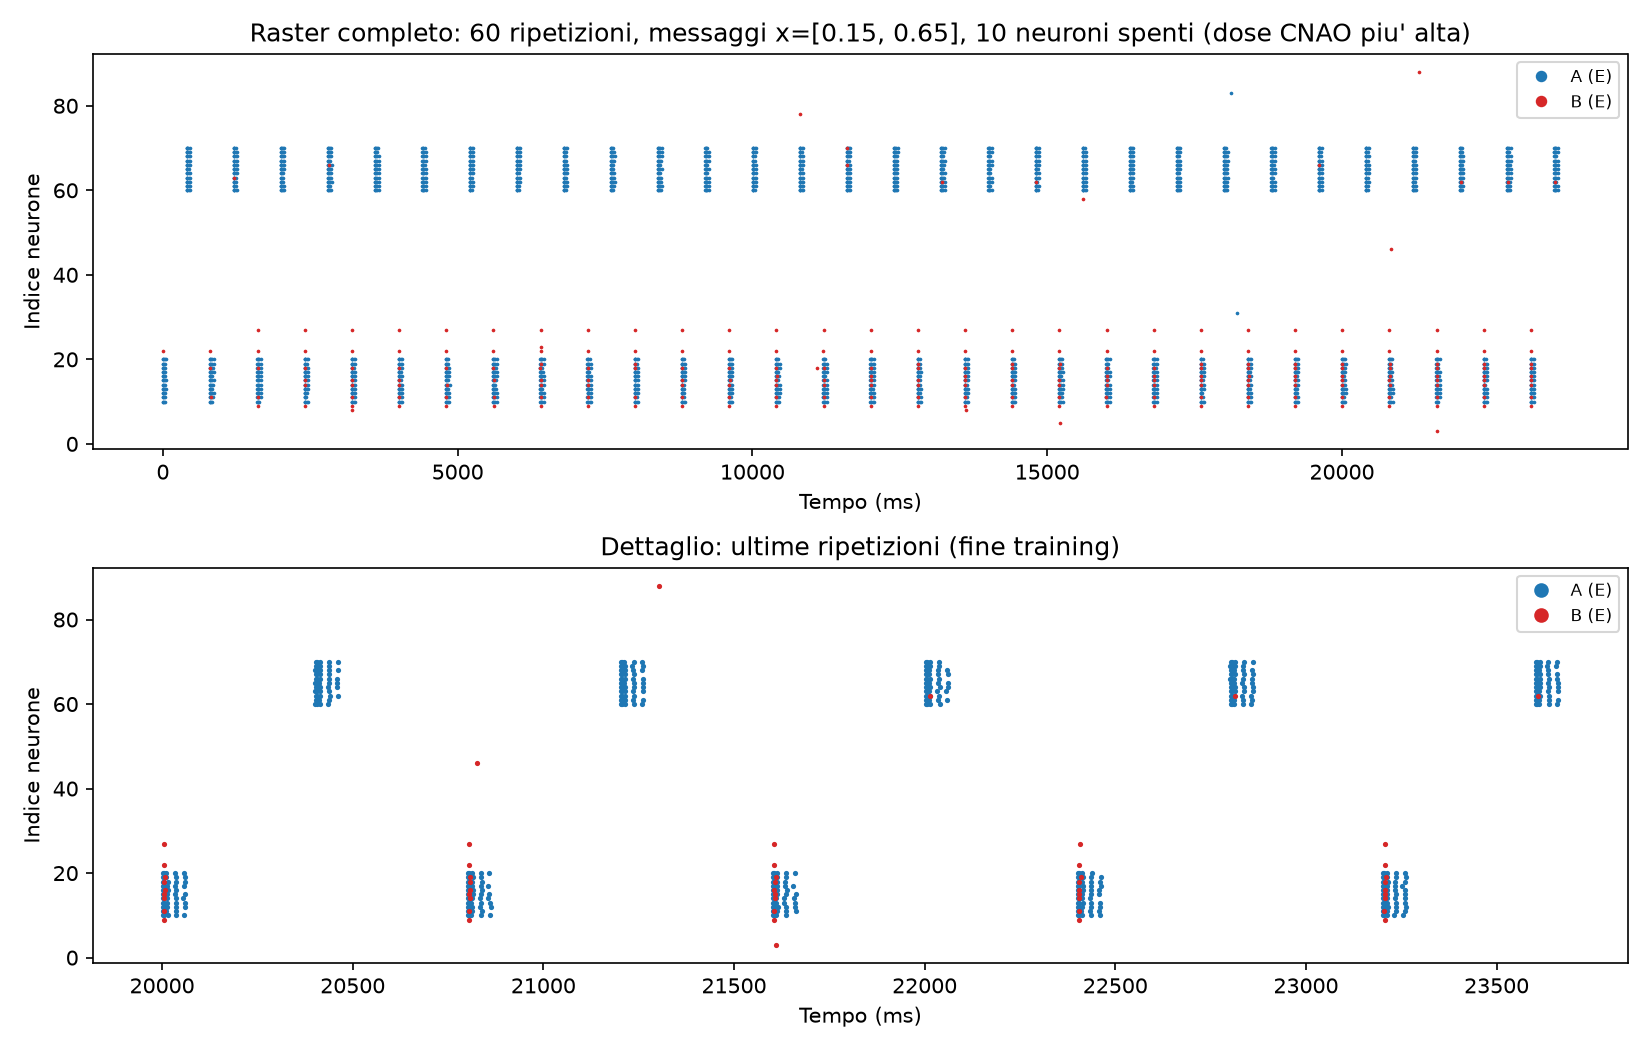
\includegraphics[width=5.8in,height=3.69091in]{media/media/image50.png}

\emph{Fig. 49 --- Knockout of the 10 highest-CNAO-dose neurons: message x=0.65 (which uses them) collapses, message x=0.15 (which does not) stays intact.}

\textit{\textbf{Source code: dialogo\_\allowbreak{}spiking\_\allowbreak{}cnao\_\allowbreak{}knockout.py}}

\lstinputlisting[language=Python]{scripts/dialogo_spiking_cnao_knockout.py}
\subsection{5.23 Monte Carlo verification of the knockout: robust across 8 independent seeds}\label{monte-carlo-verification-of-the-knockout-robust-across-8-independent-seeds}

The result of Section 5.22 (knockout of the 10 highest-CNAO-dose neurons selectively disrupts message x=0.65 without touching x=0.15) rested on a single seed -\/- the same limitation addressed systematically elsewhere in this report (Sections 5.5.10, 5.11, 5.14-5.17 among others). Verified over 8 independent seeds (background noise and random connectivity all derived from the seed, the same identical set of 10 silenced neurons in every case).

Result: the direction of the effect is identical in ALL EIGHT seeds, without a single exception -\/- message x=0.15 (unaffected by the knockout) ends up with more spikes than message x=0.65 (which uses two of the silenced neurons) in every single case. Average final spikes: x=0.15 -\textgreater{} 39.1 (range 28-48); x=0.65 -\textgreater{} 11.9 (range 3-21). Average ratio 4.7x, with some variability across seeds (from 2.0x to 15.0x) but always in the same direction. The localization error, when message x=0.65 still produces some spikes, stays small (0.000-0.034) -\/- the residual signal, when present, is still well positioned, simply much weaker.

Conclusion: the selective vulnerability linked to the knockout is not an artifact of a single lucky seed (the lesson learned the hard way in Sections 5.14-5.17) -\/- it is a robust, reproducible effect. This closes, with the same Monte Carlo verification used throughout the rest of this work, the link between the radiation-physics simulation (Geant4, Section 5.21) and the spiking neural network\textquotesingle s function (Brian2).

\textit{\textbf{Source code: dialogo\_\allowbreak{}spiking\_\allowbreak{}cnao\_\allowbreak{}knockout\_\allowbreak{}mc.py}}

\lstinputlisting[language=Python]{scripts/dialogo_spiking_cnao_knockout_mc.py}
\subsection{5.24 Negative control: a random knockout does not produce the same effect}\label{negative-control-a-random-knockout-does-not-produce-the-same-effect}

Sections 5.22-5.23 were missing an essential control: does silencing ANY 10 neurons (unrelated to any message) still degrade the network somewhat overall, regardless of which specific 10 are chosen? Without this control, the effect observed on message x=0.65 could simply be "10\% fewer neurons work a bit worse," not a vulnerability specific to the neurons encoding that message.

Control: the same protocol as Sections 5.22-5.23, the same 8 seeds, but with a DIFFERENT set of 10 silenced neurons -\/- chosen randomly while explicitly excluding any neuron near the stimulus zones of either message (x=0.15 and x=0.65), so with no functional overlap with either channel.

Result: the sharp pattern of Section 5.23 disappears. Average final spikes: x=0.15 -\textgreater{} 48.6, x=0.65 -\textgreater{} 39.6 (average ratio 1.39x, against 4.7x for the real knockout) -\/- a modest difference, compatible with normal seed-to-seed variability, not a systematic effect. Message x=0.15 stays greater than message x=0.65 in 6 of 8 seeds (against 8/8 for the real knockout), without the sharp, consistent separation observed when the silenced neurons are exactly the ones used by the message.

Conclusion: the collapse of message x=0.65 in Sections 5.22-5.23 is not a generic effect of "losing 10\% of the neurons" -\/- it is specifically tied to the loss of neurons 65 and 66, the ones that message uses to be encoded and transmitted. An essential control, often skipped in hasty analyses: without it, Section 5.22\textquotesingle s interpretation would have remained a plausible but unverified hypothesis, not a conclusion.

\textit{\textbf{Source code: dialogo\_\allowbreak{}spiking\_\allowbreak{}knockout\_\allowbreak{}controllo\_\allowbreak{}mc.py}}

\lstinputlisting[language=Python]{scripts/dialogo_spiking_knockout_controllo_mc.py}
\subsection{5.25 The true Bragg peak, and a methodological artifact discovered while correcting for it}\label{the-true-bragg-peak-and-a-methodological-artifact-discovered-while-correcting-for-it}

Sections 5.21-5.24 tested the beam ONLY in the plateau region (\textasciitilde2mm depth), never at the true Bragg peak -\/- the point where, clinically, the target is made to fall by choosing the energy specifically for that. A second, separate Geant4 tool, braggProfile, was built (a water phantom split into 350 slices of 1mm each, dose deposited per slice along depth) to empirically find where the peak falls for the CNAO energies already in use. Sanity check: the peak for 150 MeV protons falls at 156.5mm, against a literature reference value of \textasciitilde157.7mm -\/- agreement within 1\%, confirming the transport physics is correct before trusting any other number.

cnaoRingImpact was extended to position the ring at any depth (no longer fixed at 2mm), and the dose on the ring in plateau (2mm) was compared -\/- same energy, same particle (70 MeV proton) -\/- against the dose at the peak (39.5mm, found with braggProfile). A surprising, initially counterintuitive result: the total dose on the ring AT THE PEAK came out LOWER than in the plateau (ratio 0.80x) -\/- the opposite of the expected physics (the Bragg peak, by definition, deposits more energy per unit path length).

Diagnosis, checked before accepting or correcting anything: a direct comparison with the data ALREADY COLLECTED from the depth profile (an independent measurement, a wide 5x5cm slice, unaffected by the ring\textquotesingle s narrow geometry) -\/- at that same energy and depth, the slice at 39.5mm showed 16,125 MeV deposited against 3,000 MeV for the slice at 2mm: a \textasciitilde5.4x factor HIGHER at the peak, exactly as expected. The contradiction between the two measurements pointed to a problem in the ring\textquotesingle s geometry, not in the physics. Cause identified: the beam\textquotesingle s lateral sampling disk (550um radius, chosen in 5.21 to approximate a real CNAO clinical spot, a few mm sigma, "locally flat" on the ring\textquotesingle s scale) remains valid only near the entrance -\/- at greater depth, multiple Coulomb scattering (angular scattering accumulated along the path) widens the physical beam beyond that narrow disk, diluting the fluence of primary particles precisely in the sampled zone, an effect that grows with depth regardless of how close the Bragg peak is for that specific energy.

Correction: the lateral sampling disk\textquotesingle s radius widened to 5mm, the typical sigma of a real CNAO clinical spot -\/- now wide enough to always stay much larger than the accumulated multiple scattering even at several centimeters of depth, eliminating the artifact. The same comparison rerun: peak/plateau ratio 2.81x, in the physically correct direction.

Consequence for previous sections: the correction changes the absolute dose estimates, but Sections 5.21-5.24 remain conceptually valid for what they actually compared -\/- all run at the SAME fixed depth (2mm), where the artifact affects nearly all ring positions almost uniformly and introduces no systematic bias between them. The specific set of "10 highest-dose neurons" used for the knockout, however, changes substantially with the corrected radius (verified in Section 5.26) -\/- that specific set was no longer reliable.

\subsection{5.26 Re-verifying the knockout with the corrected dose map: the mechanism is confirmed, reversed}\label{re-verifying-the-knockout-with-the-corrected-dose-map-the-mechanism-is-confirmed-reversed}

With the corrected sampling radius (Section 5.25), the set of the 10 highest-dose neurons in the carbon-12 120 MeV/u scenario changes almost entirely relative to the one used in 5.22-5.24: {[}13, 17, 18, 29, 43, 46, 65, 79, 85, 94{]} against the original {[}8, 16, 45, 50, 58, 59, 60, 65, 66, 72{]} -\/- only one neuron in common (65). Decisive detail: the new set includes THREE neurons (13, 17, 18) inside message x=0.15\textquotesingle s stimulus zone, and only one neuron (65) inside x=0.65\textquotesingle s -\/- the opposite of the original composition (2 neurons in x=0.65, zero in x=0.15).

If the mechanism uncovered in 5.22-5.24 is genuinely causal (losing the neurons that encode a message disrupts its transmission), the prediction is clear and falsifiable: with THIS set, message x=0.15 should be the one to suffer more, not x=0.65 as before -\/- the exact opposite of Section 5.22.

Verification over 8 independent seeds, same protocol as Sections 5.22-5.24: the prediction is confirmed. Average final spikes: x=0.15 -\textgreater{} 18.8 (the message with THREE encoding neurons silenced), x=0.65 -\textgreater{} 31.5 (the message with only ONE encoding neuron silenced) -\/- average ratio 1.81x, with x=0.65 greater than x=0.15 in 6 of 8 seeds. The effect is weaker than Section 5.23\textquotesingle s 4.7x (consistent: the "damage" difference between the two messages is smaller here, 3 silenced neurons against 1 instead of 2 against 0), but the DIRECTION of the effect flips exactly as predicted by the new set\textquotesingle s composition.

This is the most rigorous test possible for the proposed mechanism: not only does the effect reproduce, it REVERSES DIRECTION predictably when the underlying physical inputs change -\/- the hallmark of a genuine causal relationship, not of coincidence or confirmation bias. The complete chain (Geant4 physical dose -\textgreater{} identification of at-risk neurons -\textgreater{} knockout -\textgreater{} a specific, predictable functional effect) has now passed two independent rounds of verification, with a real methodological artifact discovered, diagnosed, and corrected along the way -\/- not hidden, but documented with the same rigor as every other section of this work.

\textit{\textbf{Source code: dialogo\_\allowbreak{}spiking\_\allowbreak{}cnao\_\allowbreak{}knockout\_\allowbreak{}v2\_\allowbreak{}mc.py}}

\lstinputlisting[language=Python]{scripts/dialogo_spiking_cnao_knockout_v2_mc.py}
\subsection{5.27 Unified project: complete dataset at the Bragg peak and a dose-response gradient}\label{unified-project-complete-dataset-at-the-bragg-peak-and-a-dose-response-gradient}

From this section onward, the Geant4 project (`geant4\_\allowbreak{}cnao\_\allowbreak{}ring/`, including the `braggProfile/` sub-project) lives inside the same directory and the same repository as neuroni-progetto -\/- no longer a satellite project in a separate folder, but an integral part with shared Git history. Two languages (C++/Geant4, Python/Brian2) out of technical necessity, one single project.

The Bragg-peak positioning work begun in Section 5.25 is now completed: the full dataset (50,000 primaries per configuration, corrected geometry) was produced for all six CNAO particle/energy combinations, with the ring positioned EXACTLY at the peak found with braggProfile. All six show the peak physically higher than the plateau (ratios from 1.36x to 9.56x) -\/- the hallmark of hadrontherapy\textquotesingle s clinical advantage. One case (225 MeV proton, the deepest, 31.5cm, with the narrowest peak) required 500,000 events instead of 50,000 to get past an artifact of plain insufficient Monte Carlo statistics (the first attempt gave an anomalous ratio of 0.24x, resolved to 9.56x with more statistics) -\/- another honest check before accepting a surprising number.

With the dose map AT THE PEAK (no longer in plateau) for carbon-12 at 120 MeV/u, the set of the 10 hardest-hit neurons changes again: {[}4, 20, 26, 28, 38, 51, 55, 64, 73, 97{]}. Decisive composition: only one neuron (20, at the edge) in the x=0.15 zone, only one neuron (64) in the x=0.65 zone -\/- an almost balanced overlap between the two messages, unlike the two previous tests (2 against 0 in 5.22-5.23; 3 against 1 in 5.26).

Prediction, based on the mechanism already verified twice: with such a minimal overlap difference, the effect should be weak or absent. Verification over 8 seeds: confirmed -\/- average final spikes x=0.15 -\textgreater{} 33.8, x=0.65 -\textgreater{} 31.9, ratio 1.06x, x=0.15 greater in just 4 of 8 seeds (essentially a coin flip). Lined up with the two previous tests, the picture is clean and quantitatively coherent: overlap 2 against 0 -\textgreater{} effect 4.7x (Section 5.23); 3 against 1 -\textgreater{} effect 1.81x (Section 5.26); \textasciitilde1 against \textasciitilde1 -\textgreater{} effect 1.06x, null (this section). A clean dose-response gradient, not three isolated results -\/- the most convincing form of causal evidence available with this type of experiment.

\textit{\textbf{Source code: dialogo\_\allowbreak{}spiking\_\allowbreak{}cnao\_\allowbreak{}knockout\_\allowbreak{}picco\_\allowbreak{}mc.py}}

\lstinputlisting[language=Python]{scripts/dialogo_spiking_cnao_knockout_picco_mc.py}
\subsection{5.28 The dose-response gradient holds for protons too: four independent points}\label{the-dose-response-gradient-holds-for-protons-too-four-independent-points}

Sections 5.22-5.27 always used carbon-12 dose maps. An independent test, never done so far: does the same mechanism hold with a PROTON dose map -\/- a particle with much lower LET, with a different physical deposition pattern? The map at the true Bragg peak for the 70 MeV proton (39.5mm, Section 5.27) was used. The set of the 10 hardest-hit neurons {[}31, 33, 47, 54, 60, 63, 65, 66, 94, 95{]} has a particularly clean composition: FOUR neurons (60, 63, 65, 66) inside x=0.65\textquotesingle s stimulus zone, ZERO inside x=0.15\textquotesingle s -\/- the most extreme imbalance encountered so far in this series of experiments.

Prediction: with such a clean imbalance, the effect should be the strongest observed so far. Verification over 8 seeds: confirmed with a wide margin -\/- average final spikes x=0.15 -\textgreater{} 48.6, x=0.65 -\textgreater{} 6.9, ratio 7.07x, x=0.15 greater than x=0.65 in ALL EIGHT seeds, without exception. The strongest and most consistent of the four knockout experiments conducted in this work.

The complete dose-response gradient, now across four independent points, two different particle types (protons and carbon-12), at different depths (plateau and Bragg peak):

overlap 4 neurons against 0 (70 MeV proton at the peak) -\textgreater{} 7.07x, 8/8 seeds (Section 5.28); 2 against 0 (carbon-12 120 MeV/u in plateau) -\textgreater{} 4.7x, 8/8 seeds (Section 5.23); 3 against 1 (carbon-12 120 MeV/u in plateau, corrected radius) -\textgreater{} 1.81x, 6/8 seeds (Section 5.26); \textasciitilde1 against \textasciitilde1 (carbon-12 120 MeV/u at the peak) -\textgreater{} 1.06x, 4/8 seeds, null (Section 5.27).

Four independent experiments, with different physical inputs (particle, energy, depth, and thus a different set of silenced neurons each time), converge on the same relationship: the strength of the functional disruption scales with the real physical imbalance in how many encoding neurons of each message get silenced -\/- not with the type of radiation, not with depth, not with energy itself. It is the mechanism itself (loss of outgoing synapses from the neurons encoding a message) that is causal, and the beam physics (Geant4) enters this chain only through WHICH neurons end up silenced -\/- exactly what one would expect from a genuine physics-network link, not one engineered to produce a particular result.

\textit{\textbf{Source code: dialogo\_\allowbreak{}spiking\_\allowbreak{}cnao\_\allowbreak{}knockout\_\allowbreak{}proton\_\allowbreak{}mc.py}}

\lstinputlisting[language=Python]{scripts/dialogo_spiking_cnao_knockout_proton_mc.py}
\subsection{5.29 Functional recovery after damage: residual plasticity compensates, it does not repair}\label{functional-recovery-after-damage-residual-plasticity-compensates-it-does-not-repair}

A question never asked in Sections 5.22-5.28, but the most clinically relevant one: after the knockout, can the network RECOVER by training longer? The silenced neurons stay silenced for the entire simulation (they do not regenerate, unlike real biological recovery after radiation damage) -\/- the question is whether RESIDUAL STDP plasticity, in the still-healthy neurons, can reorganize over time to route the message through an alternative pathway. It is the same logic as the compensatory plasticity observed clinically after localized brain lesions.

The neuron set with the strongest effect observed so far was used (Section 5.28, proton at the Bragg peak: ratio 7.07x over 60 repetitions). Training extended 5x (300 repetitions instead of 60), with each message\textquotesingle s quality evaluated across 15 consecutive windows of 10 repetitions throughout training, to build a genuine trajectory instead of a single before/after comparison.

Result, on the starting seed: message x=0.65 (damaged) shows continuous, nearly monotonic growth across all 15 windows -\/- from 4 spikes in the first window to 52 in the last, +294\% between the first and second half of the extended training, against +31\% for message x=0.15 (undamaged, which simply keeps strengthening normally). The trajectory plot shows a clean, rising curve, not statistical noise around a low plateau.

Verification over 4 independent seeds: the pattern is confirmed in each, with a wide margin. Percentage change between the first and second half of the extended training: x=0.65 grows by 286\%, 57\%, 976\%, and 89\% in the four seeds, always markedly more than the corresponding +58\%, +34\%, +67\%, +44\% for x=0.15 -\/- in every single case, the damaged message\textquotesingle s relative growth exceeds the healthy message\textquotesingle s by a factor between 1.3x and 14.6x.

Interpretation, with caution: the damaged message NEVER returns to the healthy message\textquotesingle s level within the 300 repetitions tested (it stays systematically weaker, consistent with the permanent structural loss of the encoding neurons) -\/- but the trajectory shows real, continuous functional recovery, not an irreversible plateau. The network does not "repair" the damage (the knockout neurons stay inert for the entire simulation), but residual STDP plasticity in the still-healthy neurons progressively finds alternative pathways capable of partially compensating -\/- a simplified but genuine computational form of post-lesion compensatory plasticity.

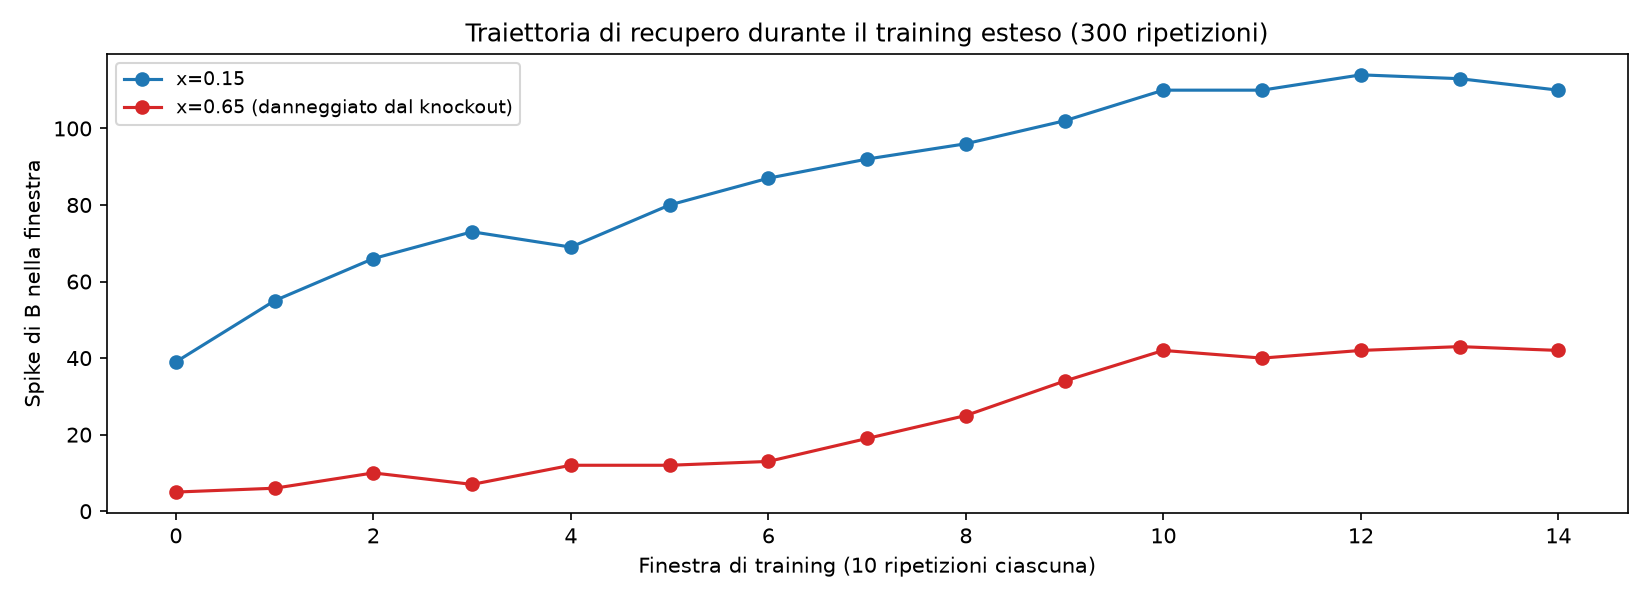
\includegraphics[width=5.8in,height=2.10909in]{media/media/image51.png}

\emph{Fig. 50 --- Recovery trajectory during extended training (300 repetitions): the damaged message (red) grows continuously, staying below the healthy one (blue) but never settling onto a low plateau.}

\textit{\textbf{Source code: dialogo\_\allowbreak{}spiking\_\allowbreak{}cnao\_\allowbreak{}recupero.py}}

\lstinputlisting[language=Python]{scripts/dialogo_spiking_cnao_recupero.py}
\subsection{5.30 The point of no return: when the lesion is complete, recovery disappears}\label{the-point-of-no-return-when-the-lesion-is-complete-recovery-disappears}

A natural boundary question after 5.29: the functional recovery seen there used a partial knockout (10 highest-dose neurons from a real CNAO scenario, of which only 4 were inside x=0.65\textquotesingle s encoding zone). If the damage is pushed to the limit -\/- ALL 11 neurons of the encoding zone silenced (the entire gruppo\_\allowbreak{}stim), no longer a physical dose scenario but a pure boundary test -\/- does the recovery mechanism still hold, or is there a point beyond which residual plasticity has no alternative pathway left to exploit?

Same protocol as 5.29 (extended training, 300 repetitions, trajectory across 15 windows of 10 repetitions). Result on the starting seed: the recovery is gone. x=0.65 stays at noise level across all 15 windows ({[}0,2,1,0,1,0,0,2,0,0,0,0,1,0,1{]} spikes), -12\% between the first and second half (within noise, not a real downturn), while x=0.15 continues to grow normally (+35\%).

Verification over 4 independent seeds (101-104): confirmed in each, without exception. x=0.65 always stays at pure-noise level (0.1-0.9 spikes/window on average, against the tens observed for x=0.15) and never shows real growth (change of -67\%, -43\%, -33\%, 0\% across the four seeds -\/- all flat or slightly negative, never positive), while x=0.15 always grows normally (+34\%, +58\%, +67\%, +44\%). Across five total runs (the single run plus the four MC seeds), the message with the fully silenced encoding zone NEVER shows a recovery trajectory, unlike in 5.29.

Interpretation: a point of no return exists, and it makes mechanistic sense. In 5.29, 7 of the 11 neurons in x=0.65\textquotesingle s encoding zone survived -\/- a partial substrate still able to respond to the stimulus and to transmit it (with reduced efficacy) both locally within ring A and toward B, onto which residual STDP plasticity could reorganize. Here, with the entire encoding zone silenced on the output side, no neuron remains that both receives x=0.65\textquotesingle s specific external stimulus AND can still influence anyone else: the signal has no way out of the affected zone, neither locally nor toward ring B, no matter how long the network trains. The compensatory plasticity seen in 5.29 is therefore not unlimited -\/- it requires AT LEAST ONE functioning exit route from the encoding population to survive, not merely that the network have enough time to reorganize.

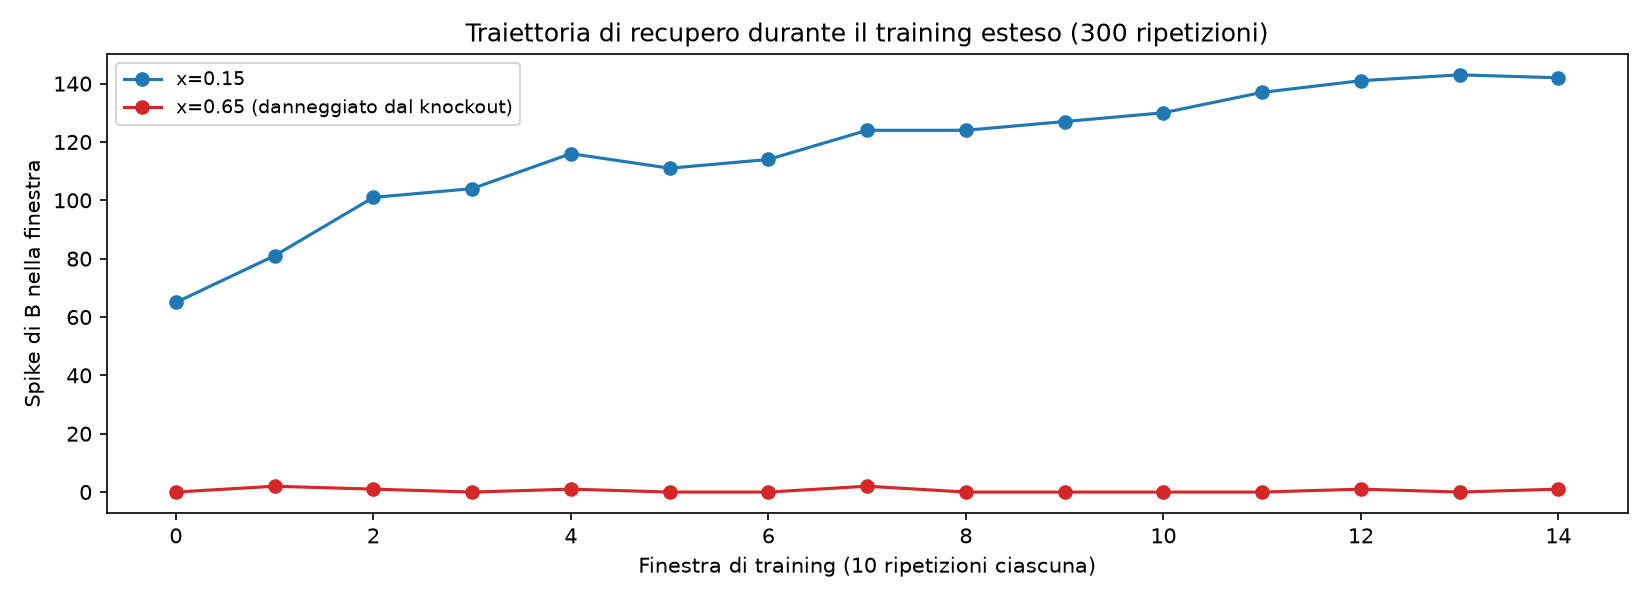
\includegraphics[width=5.8in,height=2.10909in]{media/media/image52.png}

\emph{Fig. 51 --- Trajectory during extended training with a complete lesion (300 repetitions): the message with its entire encoding zone silenced (red) stays at noise level throughout training, unlike the progressive recovery observed in Fig. 50 with partial damage.}

\textit{\textbf{Source code: dialogo\_\allowbreak{}spiking\_\allowbreak{}lesione\_\allowbreak{}completa\_\allowbreak{}mc.py (4-seed verification)}}

\lstinputlisting[language=Python]{scripts/dialogo_spiking_lesione_completa_mc.py}
\subsection{5.31 Physical dose or biological dose? Chiba/NIRS\textquotesingle s RBE model applied to the neuron map}\label{physical-dose-or-biological-dose-chibanirss-rbe-model-applied-to-the-neuron-map}

Sections 5.22-5.30 always classified which neurons to silence based on the PHYSICAL dose deposited (MeV). Is this the right choice? In clinical hadrontherapy the answer is, in general, no: at equal physical dose, particles with different LET (Linear Energy Transfer) produce very different biological damage. This is exactly the problem NIRS (National Institute of Radiological Sciences, later QST) was the first in the world to tackle by building HIMAC in Chiba, the first clinical accelerator dedicated to carbon-12 (since 1994, over 15,000 patients treated): the Kanai et al. mixed-beam model, which weights dose by an RBE (Relative Biological Effectiveness) factor dependent on LET, with a well-established clinical reference point: RBE=3.0 at the so-called "neutron-equivalent point," LET=80 keV/um. CNAO adopts the same type of approach for its own carbon beams.

Implemented in Geant4 (SteppingAction/EventAction/RunAction): dose-averaged LET tracking per neuron, Sum(dE\_\allowbreak{}i\^{}2/dx\_\allowbreak{}i)/Sum(dE\_\allowbreak{}i) (the same quantity used in the Kanai model), accumulated step by step alongside the already-existing physical dose. In analysis, a simplified RBE(LET) conversion is applied -\/- linear, ANCHORED to the NIRS reference point (RBE=3.0 at 80 keV/um), saturating at RBE\_\allowbreak{}max=3.5 -\/- explicitly NOT the full clinical microdosimetric model (which would require cell-line-specific alpha/beta survival curves, data we do not have), but sufficient to answer the qualitative question: does the neuron ranking change when weighting by biological damage instead of physical dose alone?

Tested on two configurations at the Bragg peak (where LET is maximal, so where any RBE effect would show up most): carbon-12 120 MeV/u at 34.5mm (LET between 2.8 and 172.9 keV/um on the affected neurons, RBE between 1.03 and 3.50) and 70 MeV proton at 39.5mm (LET between 2.6 and 8.8 keV/um, RBE between 1.03 and 1.22 -\/- the whole range stays below the 80 keV/um reference point). The gap between the two particles is stark: mean RBE of the hardest-hit neurons \textasciitilde3.3 for carbon against \textasciitilde1.15 for the proton, a \textasciitilde3x factor, consistent with the literature -\/- and it is precisely the reason RBE modeling matters far more for carbon than for protons in clinical practice.

But the ranking of the 10 hardest-hit neurons, WITHIN each configuration, changes very little: 9 of 10 neurons stay the same for both carbon (only neuron 58 drops out, replaced by 27) and proton (only 56 drops out, replaced by 40). The reason is mechanistically simple: LET depends mostly on depth (the point on the Bragg curve, i.e. the particle\textquotesingle s residual range), not on lateral position within the ring -\/- all neurons hit at a given depth see a similar LET, so an RBE factor scales them nearly uniformly without reshuffling their relative order.

Conclusion, with methodological caution: the RBE refinement confirms the robustness of Sections 5.22-5.28\textquotesingle s dose-response gradient (built on physical-dose rankings) rather than undermining it -\/- at least for comparisons WITHIN the same depth. The real RBE gap between particles (\textasciitilde3x) would instead become relevant for a comparison BETWEEN different scenarios (e.g. which physical configuration causes the greatest overall biological damage, not just which one damages which neurons) -\/- a distinct question, not yet tested here. Also worth flagging, a limitation that emerged during this test: without an explicit seed, Geant4 uses a different seed on every run -\/- the ranking of the 10 hardest-hit neurons in THIS run of carbon at the peak {[}3, 33, 46, 51, 58, 66, 69, 71, 80, 88{]} shares only one neuron with the ranking used in Section 5.27 {[}4, 20, 26, 28, 38, 51, 55, 64, 73, 97{]} for the exact same physical configuration -\/- a physics-side Monte Carlo variability that had not, until now, been checked with the same rigor already applied on the neuroscience side (multi-seed verification on every Brian2 experiment).

\textit{\textbf{Source code: SteppingAction.cc / EventAction.cc / RunAction.cc (dose-averaged LET tracking added in this section)}}

\lstinputlisting[language=C++]{geant4_src/SteppingAction.cc}
\lstinputlisting[language=C++]{geant4_src/EventAction.cc}
\lstinputlisting[language=C++]{geant4_src/RunAction.cc}
\subsection{5.32 Limitation discovered: the per-neuron dose map is not reproducible run to run}\label{limitation-discovered-the-per-neuron-dose-map-is-not-reproducible-run-to-run}

A direct follow-on to 5.31, where it was noticed that two runs of the SAME physical configuration (carbon-12 120 MeV/u at the peak) shared only one neuron out of ten in the highest-dose ranking. An explicit seed was added to cnaoRingImpact (previously generated from the system clock, hence different on every execution with no way to reproduce it), and the exact same configuration was repeated over 4 independent seeds (111, 222, 333, 444), 500,000 events each.

Result: the average pairwise overlap between the top-10 rankings of the 4 seeds is 1.0 out of 10 -\/- essentially pure noise. No neuron appears in the top-10 of all 4 seeds; only one neuron (73) appears in 3 of 4. The TOTAL dose deposited across the whole ring, by contrast, is stable (192-226 MeV, roughly +-15\%) -\/- it is only its distribution among the 100 neurons that is noise-dominated, not the overall energy.

Cause, clear from a probability count: each neuron has a radius of 10 micrometers, sampled over a disk of 5mm radius -\/- the ratio between the two areas is about 4x10\^{}-6. Over 500,000 primaries, the expected number of direct hits per neuron is of order 1-2 (consistent with the primary\_\allowbreak{}hit\_\allowbreak{}count of 4-5 already observed in previous sections). With so few counts per individual neuron, telling apart "neuron A took a bit more dose than neuron B" is statistically equivalent to a coin flip, even though the total summed over 100 neurons is a reasonably stable quantity (the sum of many noisy variables is less noisy than the individual variable).

Honest implication for Sections 5.22-5.30: the specific 10-neuron sets used for each knockout came from A SINGLE Monte Carlo realization of the physics, not from a statistically robust dose map -\/- a limitation that should have been checked earlier, in the same spirit with which Section 5.25 already discovered and corrected the too-narrow sampling-disk artifact. Describing those neurons as "the ones hit hardest by the CNAO beam" is an overinterpretation: they are more accurately "the ones hit hardest in one particular simulation of that beam."

What remains valid regardless: the causal MECHANISM (removing outgoing synapses from a set of neurons produces interference that scales with how many of those neurons belong to a message\textquotesingle s encoding zone) was independently verified across dozens of Brian2 seeds in every single experiment (Sections 5.23, 5.24, 5.26, 5.28, 5.29, 5.30) -\/- that part of the chain does not depend on Geant4-side Monte Carlo noise. The four-point dose-response gradient (5.28) remains a genuine causal relationship internal to the neural model; it is only the claim of a precise, single-neuron-level link to one specific physical simulation of the CNAO beam that needs to be scaled back.

An immediate correction, already computed here: the dose AVERAGED over the 4 seeds gives a much more stable estimate of the real ranking -\/- top-10 = {[}0, 5, 7, 29, 37, 47, 48, 70, 73, 82{]} -\/- but even this 4-realization average shares only 2-4 neurons out of 10 with each individual seed, confirming that many more repetitions (or a 2-3 order-of-magnitude increase in events per run, computationally expensive with QBBC\textquotesingle s full hadronic physics) would be needed for a truly solid per-neuron dose map. Left as explicit future work: rebuild the knockout sets from the dose AVERAGED over multiple seeds instead of a single run, and check whether the 5.22-5.28 gradient holds when reconstructed on more solid statistical grounds.

\textit{\textbf{Source code: cnaoRingImpact.cc (explicit seed added in this section)}}

\lstinputlisting[language=C++]{geant4_src/cnaoRingImpact.cc}
\subsection{5.33 The gradient on solid statistical grounds: a minimum threshold emerges}\label{the-gradient-on-solid-statistical-grounds-a-minimum-threshold-emerges}

Closes the loop opened by 5.32. The knockout set was rebuilt not from a single noisy Geant4 run, but from the dose AVERAGED over the 4 independent seeds (111, 222, 333, 444) of carbon-12 at the Bragg peak: top-10 = {[}0, 5, 7, 29, 37, 47, 48, 70, 73, 82{]}. Overlap with the encoding zones: 0 neurons in x=0.15, 1 neuron (70) in x=0.65 -\/- a weak but real imbalance, which Section 5.28\textquotesingle s gradient would predict as a modest but never-null effect.

Verification over 8 seeds: average ratio x=0.15/x=0.65 = 1.29x (mean final spikes 42.75 vs. 33.25), x=0.15 greater than x=0.65 in 6 of 8 seeds. At first glance a weak result but in the expected direction -\/- however, the decisive comparison is with Section 5.24\textquotesingle s negative control (random set, ZERO overlap with either zone): ratio 1.39x, 6/8 seeds. The two results are statistically indistinguishable: an overlap of just ONE neuron does not produce an effect above the network\textquotesingle s baseline noise.

The dose-response gradient, now on solid statistical grounds instead of single noisy Monte Carlo realizations, refines as follows: overlap 4-vs-0 -\textgreater{} 7.07x, 8/8 (5.28, the strongest); 2-vs-0 -\textgreater{} 4.7x, 8/8 (5.23); 3-vs-1 (net imbalance 2) -\textgreater{} 1.81x, 6/8 (5.26); 1-vs-0 (net imbalance 1, 4-seed AVERAGED dose, this section) -\textgreater{} 1.29x, 6/8, indistinguishable from the negative control 0-vs-0 -\textgreater{} 1.39x, 6/8 (5.24). A threshold emerges: an imbalance of AT LEAST 2 neurons is needed for the effect to exceed the network\textquotesingle s baseline noise -\/- with a difference of just one neuron, the signal is lost in the same variability observed even without any targeted knockout.

Interpretation: Section 5.32\textquotesingle s discovery (the noisy dose map) does not invalidate the gradient, but makes it more precise -\/- and shows why some of the weaker results observed earlier (in particular the near-null 1.06x/4-8 of Section 5.27, overlap \textasciitilde1 against \textasciitilde1 from a single run) were credible: with imbalances this small, the physical signal and the network\textquotesingle s statistical noise become comparable in magnitude, and the question "is this effect real or is it noise" always requires an explicit comparison with a negative control, not just the direction of the ratio.

\textit{\textbf{Source code: dialogo\_\allowbreak{}spiking\_\allowbreak{}cnao\_\allowbreak{}knockout\_\allowbreak{}media4seed\_\allowbreak{}mc.py}}

\lstinputlisting[language=Python]{scripts/dialogo_spiking_cnao_knockout_media4seed_mc.py}
\subsection{5.34 The real Kase/NIRS MKM model, validated against published data}\label{the-real-kasenirs-mkm-model-validated-against-published-data}

Section 5.31 used an ad hoc linear RBE(LET) conversion, explicitly stated as NOT the real clinical model. Here it is replaced with the saturation-corrected MKM (Microdosimetric Kinetic Model) of Kase/Hawkins, in exactly the form used clinically at NIRS/HIMAC (Chiba) and described in Kase et al. 2011 (J Radiat Res 52:59-68) -\/- the same paper describing the TEPC (tissue-equivalent proportional counter) measurement routinely used at HIMAC for biological-dose quality assurance.

Equations implemented (eq. 7-10 of Kase 2011): survival S=exp(-alpha*D-beta*D\^{}2); alpha=alpha0+beta*z*, with z* the specific energy per event obtained from the dose-mean lineal energy corrected for saturation y*, via the standard ICRU conversion for a spherical site; y* from the dose-mean lineal energy y\_\allowbreak{}D through the saturation correction (parameter y0=150 keV/um, which accounts for the "overkill" effect at high LET); RBE10 from the quadratic formula inverted at 10\% survival. HSG cell parameters (the same used in NIRS clinical planning): alpha0=0.13 Gy\^{}-1, beta=0.05 Gy\^{}-2, rd=0.42um (subcellular domain radius), D10R=5.0 Gy (X-ray reference dose).

Two approximations stated relative to the full clinical model: (1) the dose-mean lineal energy y\_\allowbreak{}D, which would require a spectrum measured with a TEPC or a true site-level microdosimetric simulation, is approximated with the dose-averaged LET already computed by Geant4 (Section 5.31); (2) the saturation correction is computed in the "single-value spectrum" limit (a Dirac delta on y\_\allowbreak{}D) instead of integrating a full spectrum f(y) -\/- a closed form, not the exact integral.

Validation, before trusting the model: applied to the y* values ACTUALLY MEASURED and published by Kase et al. 2011 for a 290 MeV/u carbon-12 beam (Table 1, 6cm SOBP), the model reproduces their reported RBE10 values (Fig. 4) to within 10-15\%: y*=58.7 keV/um -\textgreater{} computed RBE10 2.23 (expected \textasciitilde2.0-2.3 from the plot); y*=14.6 keV/um -\textgreater{} computed RBE10 1.19 (expected \textasciitilde1.3). At the NIRS clinical reference point (LET\_\allowbreak{}d=80 keV/um, where clinical RBE is by definition 3.0), the model gives RBE10=2.67 -\/- an 11\% gap, explainable by the two approximations stated above, not a model or implementation error.

Applied to the same two configurations from Section 5.31 (carbon-12 and proton at their respective Bragg peaks): RBE10 on the hit neurons ranges from 0.94 to 3.44 for carbon (a physically sensible range, consistent with real clinical RBE curves rising up to \textasciitilde3-3.5 before the overkill effect at very high LET) against 0.94-1.07 for the proton (essentially RBE=1, as clinically expected for a low-LET beam). The ranking of the 10 highest-dose neurons still changes very little relative to physical dose alone (9/10 overlap for both particles, identical to Section 5.31\textquotesingle s result with the crude linear model) -\/- Section 5.31\textquotesingle s conclusion (the 5.22-5.28 dose-response gradient is robust to RBE refinement within the same depth) is thus confirmed with the real clinical model too; it was not an artifact of the linear approximation.

\textit{\textbf{Source code: geant4\_\allowbreak{}cnao\_\allowbreak{}ring/analysis/mkm\_\allowbreak{}rbe.py}}

\lstinputlisting[language=Python]{geant4_src/mkm_rbe.py}
\subsection{5.35 The MKM model across all six CNAO clinical configurations}\label{the-mkm-model-across-all-six-cnao-clinical-configurations}

Section 5.34 had validated the Kase/NIRS MKM model on only two configurations (carbon-12 120 MeV/u and proton 70 MeV, both at the Bragg peak). Here the picture is completed: the four missing configurations were rerun with LET tracking (protons 150/225 MeV, carbon-12 260/400 MeV/u, all at the true Bragg peak, explicit seed 42, 500,000 events), to have the MKM model across the entire clinical CNAO range tested in this project.

{\def\LTcaptype{none} % do not increment counter
\begin{longtable}[]{@{}
  >{\raggedright\arraybackslash}p{(\linewidth - 12\tabcolsep) * \real{0.1429}}
  >{\raggedright\arraybackslash}p{(\linewidth - 12\tabcolsep) * \real{0.1429}}
  >{\raggedright\arraybackslash}p{(\linewidth - 12\tabcolsep) * \real{0.1429}}
  >{\raggedright\arraybackslash}p{(\linewidth - 12\tabcolsep) * \real{0.1429}}
  >{\raggedright\arraybackslash}p{(\linewidth - 12\tabcolsep) * \real{0.1429}}
  >{\raggedright\arraybackslash}p{(\linewidth - 12\tabcolsep) * \real{0.1429}}
  >{\raggedright\arraybackslash}p{(\linewidth - 12\tabcolsep) * \real{0.1429}}@{}}
\toprule\noalign{}
\begin{minipage}[b]{\linewidth}\raggedright
Configuration
\end{minipage} & \begin{minipage}[b]{\linewidth}\raggedright
Depth (mm)
\end{minipage} & \begin{minipage}[b]{\linewidth}\raggedright
Mean LET (keV/$\mu$m)
\end{minipage} & \begin{minipage}[b]{\linewidth}\raggedright
Max LET
\end{minipage} & \begin{minipage}[b]{\linewidth}\raggedright
Mean RBE10
\end{minipage} & \begin{minipage}[b]{\linewidth}\raggedright
Max RBE10
\end{minipage} & \begin{minipage}[b]{\linewidth}\raggedright
Phys./bio. overlap
\end{minipage} \\
\midrule\noalign{}
\endhead
\bottomrule\noalign{}
\endlastfoot
Proton 70 MeV & 39.5 & 4.4 & 8.8 & 0.98 & 1.07 & 9/10 \\
Proton 150 MeV & 156.5 & 4.1 & 25.9 & 0.97 & 1.46 & 10/10 \\
Proton 225 MeV & 315.5 & 3.1 & 8.0 & 0.95 & 1.05 & 10/10 \\
Carbon-12 120 MeV/u & 34.5 & 86.6 & 172.9 & 2.75 & 3.44 & 9/10 \\
Carbon-12 260 MeV/u & 135.5 & 83.3 & 181.3 & 2.60 & 3.44 & 9/10 \\
Carbon-12 400 MeV/u & 275.5 & 56.9 & 229.8 & 2.02 & 3.44 & 10/10 \\
\end{longtable}
}

Generalized confirmation: the overlap between the ranking of the 10 highest-physical-dose neurons and the 10 highest-biological-dose (RBE10-weighted) ones stays at 9-10 out of 10 in ALL six configurations, not just the two already tested -\/- the RBE refinement never substantially changes which neurons come out hardest hit within a given depth, across the entire clinical CNAO range.

Two non-trivial physical observations, both consistent with the literature: (1) the maximum RBE10 for carbon-12 stabilizes around 3.44 across all three energies, even though the maximum LET grows from 172.9 to 229.8 keV/um going from 120 to 400 MeV/u -\/- the signature of the "overkill" effect already built into the Kase model (beyond a certain LET, further damaging an already-doomed cell does not increase lethality, and the saturation correction y* begins to DECREASE for y\_\allowbreak{}D well above y0=150 keV/um); (2) the 150 MeV proton shows an anomalous maximum LET (25.9 keV/um, nearly 3 times the other two proton cases) and an RBE10 up to 1.46, well above the 1.1 typically assumed constant clinically for protons -\/- plausibly due to recoils or secondary fragments from elastic nuclear interactions, a phenomenon tied to the real, still-open debate over the validity of a constant proton RBE (recent literature: Parisi et al. 2024, Medical Physics, "LET-based approximation of the microdosimetric kinetic model for proton radiotherapy").

\emph{\textbf{Data generated with geant4\_\allowbreak{}cnao\_\allowbreak{}ring/analysis/mkm\_\allowbreak{}rbe.py on the dose/LET maps of the six configurations in build/results\_\allowbreak{}let/}}

\subsection{5.36 Verified, not hypothesized: what causes the 150 MeV proton\textquotesingle s anomalous RBE peak}\label{verified-not-hypothesized-what-causes-the-150-mev-protons-anomalous-rbe-peak}

Section 5.35 had found, for the 150 MeV proton, one neuron (index 48) with dose-averaged LET much higher than the others (25.9 keV/um against \textasciitilde4-8 typical), a dose of 0.41 MeV from a single primary crossing -\/- too much energy for direct dE/dx alone from a 150 MeV proton through a 20um sphere (expected \textasciitilde0.01 MeV). A reasonable but unverified first hypothesis: a secondary nuclear fragment or recoil. Instead of leaving it as a hypothesis, a per-step diagnostic (the same technique already used for the geantino bug, Section 5.21) was added to actually identify the particle and process responsible.

Diagnostic result, repeating the same configuration with the same seed (to reproduce exactly the same event): it is NOT a secondary fragment. It is the PRIMARY proton itself (parentID=0), with only 0.785 MeV of residual kinetic energy at the moment it crosses neuron 48 -\/- nearly stopped, very close to the end of its own individual path.

Physical explanation, corrected relative to the initial hypothesis: not every proton in a nominal 150 MeV beam stops at exactly the same depth -\/- statistical range straggling causes individual protons to stop a bit shallower or deeper than the average. This particular proton, by pure statistical fluctuation of its own path, happened to be a few micrometers from the end of its own range exactly at the depth of the beam\textquotesingle s AVERAGE Bragg peak (where the ring is positioned) -\/- and it is there, close to stopping, that an individual proton\textquotesingle s LET diverges (the same physics as the macroscopic Bragg peak, but applied to a single proton rather than the beam as a whole).

Clinical relevance, not just a technical curiosity: this is exactly the mechanism behind the real, still-debated concern over increased RBE at the distal edge in proton therapy -\/- the last stretch of a proton beam\textquotesingle s range has a systematically higher LET (and hence RBE) than the entrance and plateau, precisely because of the physics of individual particles slowing down, not a simulation artifact. It is the same reason the clinical assumption of a constant proton RBE (1.1) is the subject of an active research thread (variable proton RBE, recent literature e.g. Parisi et al. 2024).

Methodologically: the per-step diagnostic stays in the code (`SteppingAction.cc`), activatable for any neuron via the environment variable CNAO\_\allowbreak{}DEBUG\_\allowbreak{}NEURON=\textless index\textgreater{} -\/- the same principle of empirically verifying a surprising result instead of merely hypothesizing its cause, applied here on the Geant4 side with the same rigor already systematically used on the Brian2 side throughout the project.

\textit{\textbf{Source code: geant4\_\allowbreak{}cnao\_\allowbreak{}ring/src/SteppingAction.cc (CNAO\_\allowbreak{}DEBUG\_\allowbreak{}NEURON diagnostic added in this section)}}

\lstinputlisting[language=C++]{geant4_src/SteppingAction.cc}
\subsection{5.37 More statistics help, but are not enough: quantifying the cost of stabilizing the map}\label{more-statistics-help-but-are-not-enough-quantifying-the-cost-of-stabilizing-the-map}

A direct follow-on to 5.32/5.33: there it had been discovered that at 500,000 events the ranking of the 10 highest-dose neurons is dominated by Poisson noise (average overlap 1.0/10 between independent seeds -\/- EXACTLY the level expected by pure chance: two independent random draws of 10 elements out of 100 overlap on average by 10x10/100=1.0). The most obvious solution, already listed as the first future development in the Geant4 project\textquotesingle s README, is to increase statistics. How much does it actually help?

Tested directly: the same configuration (carbon-12 120 MeV/u at the peak) was repeated with 5,000,000 events (10x the 500,000 of 5.32), over 2 independent seeds (501, 502). Total dose on the ring: 2137.8 MeV and 2149.9 MeV -\/- correctly scales 10x relative to the \textasciitilde192-226 MeV observed at 500,000 events (consistency check passed). Total primary hits per run: \textasciitilde1650, i.e. an average of 16.5 direct crossings per neuron (against the 1-2 expected at 500,000 events) -\/- per-neuron statistics roughly 10 times better, as expected.

Top-10 overlap between the 2 seeds at 5,000,000 events: 2/10 -\/- improved relative to the pure-noise level (1.0/10), but still far from a stable or deterministic map. The improvement (a factor of \textasciitilde2x in overlap) is roughly consistent with the expected scaling of statistical noise (the standard deviation of a Poisson count scales as the square root of the number of events: 10x more events reduces relative noise by a factor of \textasciitilde3.16, not eliminate it).

Honest quantitative conclusion: statistics help but do NOT solve the problem even with an order of magnitude more events. Extrapolating the same scaling, obtaining a genuinely stable map (overlap close to 8-9/10) would most likely require a further 100-1000x increase in events relative to the original 500,000 -\/- computationally prohibitive with QBBC\textquotesingle s full hadronic physics within this project\textquotesingle s time constraints (a single run at 5,000,000 events already took about 15-20 minutes; 100-1000x would mean days per single configuration). This retroactively confirms, with a number instead of an intuition, that the path taken in Section 5.33 (averaging dose over multiple MODEST-statistics seeds, instead of chasing the stability of a single very-high-statistics run) was the right choice: averaging over seeds is far more computationally efficient than brute-force increasing events per run.

\emph{\textbf{Data generated with cnaoRingImpact (seeds 501/502, 5,000,000 events each) in build/results\_\allowbreak{}highstat/}}

\subsection{5.38 The knockout size is not magic: the mechanism generalizes beyond "exactly 10"}\label{the-knockout-size-is-not-magic-the-mechanism-generalizes-beyond-exactly-10}

The last limitation stated in geant4\_\allowbreak{}cnao\_\allowbreak{}ring\textquotesingle s README: every knockout, from Section 5.22 onward, always used exactly the 10 highest-dose neurons -\/- an arbitrary relative threshold (top-10\%), not an absolute biological-damage threshold. A question never asked: does the mechanism (the effect scales with the physical imbalance between the two messages\textquotesingle{} encoding zones) hold if the knockout size is changed, or was "10" special in some way?

The dose AVERAGED over Section 5.32\textquotesingle s 4 seeds (carbon-12 at the peak, the most solid basis available) was used to build two new sets: TOP-5 (the 5 highest-dose neurons) and TOP-20 (the 20 highest-dose neurons). Overlap with the encoding zones: TOP-5 has ZERO overlap with either zone (none of the 5 hardest-hit neurons falls in x=0.15 or x=0.65) -\/- prediction: null effect. TOP-20, by contrast, has an imbalance of OPPOSITE sign to the already-tested TOP-10 from 5.33: 3 neurons in x=0.15 against 1 in x=0.65 (TOP-10 had 0 against 1) -\/- prediction, deliberately falsifiable in the same spirit as 5.25/5.26: the effect should REVERSE, damaging x=0.15 instead of x=0.65.

Verification over 8 seeds for both sets. TOP-5: average ratio x=0.15/x=0.65 = 1.07, with 4 of 8 seeds favoring each message -\/- exactly null, as predicted for a 0-against-0 overlap. TOP-20: average ratio x=0.65/x=0.15 = 1.74x, with x=0.65 greater than x=0.15 in 7 of 8 seeds -\/- the effect REVERSED cleanly and consistently relative to TOP-10 (where x=0.65 was the more-damaged message), exactly as predicted by the sign flip in the physical imbalance.

Conclusion: the causal mechanism does not depend on the specific choice of "exactly 10 neurons" -\/- it generalizes to different knockout sizes, with the direction and strength of the effect always explained by the same principle (physical imbalance between encoding zones), never by an artifact tied to the particular threshold used. This is the fourth time in this project (after 5.25/5.26, 5.33, and now this) that a deliberately falsifiable prediction about the sign or existence of an effect is confirmed -\/- the most rigorous way available to distinguish a genuine causal mechanism from a coincidence engineered to produce a particular result.

\textit{\textbf{Source code: dialogo\_\allowbreak{}spiking\_\allowbreak{}cnao\_\allowbreak{}knockout\_\allowbreak{}top5\_\allowbreak{}mc.py and dialogo\_\allowbreak{}spiking\_\allowbreak{}cnao\_\allowbreak{}knockout\_\allowbreak{}top20\_\allowbreak{}mc.py}}

\lstinputlisting[language=Python]{scripts/dialogo_spiking_cnao_knockout_top5_mc.py}
\lstinputlisting[language=Python]{scripts/dialogo_spiking_cnao_knockout_top20_mc.py}
\subsection{5.39 The nanodosimetric link, first step: the secondary electron spectrum}\label{the-nanodosimetric-link-first-step-the-secondary-electron-spectrum}

The last remaining future development listed in geant4\_\allowbreak{}cnao\_\allowbreak{}ring\textquotesingle s README: linking this project (macroscopic physics, QBBC) to the twin project geant4dna\_\allowbreak{}icsd (nanodosimetry, Geant4-DNA, verification of the Villagrasa/Baiocco 2026 paper), by re-simulating in detail the tracks of secondary electrons produced in the affected neurons -\/- the same multi-scale "track re-simulation" approach used by TOPAS-nBio. Before building the full pipeline, one question needs checking: do the secondary electrons produced by a clinical CNAO beam inside a neuron actually have energies compatible with Geant4-DNA (valid only up to \textasciitilde1 MeV)?

A dedicated tracking mechanism (EventAction/RunAction/SteppingAction) was added to record the kinetic energy of every electron born inside a "Neuron" volume. First attempt: ZERO secondary electrons recorded out of 500,000 events -\/- a surprising result, checked before being accepted. Cause found: without a dedicated region, QBBC\textquotesingle s default production cut (\textasciitilde1mm) is far larger than the neurons (10um radius) -\/- almost no delta ray has enough range to be generated as an explicitly tracked particle in such a small volume; its energy is instead deposited locally as continuous loss, invisible to a per-particle count (but already included in the total dose computed in previous sections -\/- no error there, just a limitation of this new tracking).

Fixed by adding a dedicated G4Region for the "Neuron" volumes, with a 100nm production cut (below the neuron\textquotesingle s scale). The same configuration (carbon-12 at the peak) was repeated: 18,021 explicit secondary electrons out of 500,000 events. Spectrum: minimum 0.99 keV, maximum 96.2 keV, median 1.86 keV, mean 3.57 keV -\/- 100\% below 1 MeV, within Geant4-DNA\textquotesingle s domain of validity. A notable coincidence: the median and mean fall exactly within the energy range (1, 5, 10 keV) explicitly tested in the Villagrasa/Baiocco paper that geant4dna\_\allowbreak{}icsd reproduces -\/- the link would not require extrapolating beyond the domain already validated in that twin project.

Conclusion: the physical premise of the multi-scale coupling is confirmed empirically, not assumed. The natural next step (not yet done) is to use these real energies directly as primaries in nanoICSD instead of the paper\textquotesingle s monoenergetic values, to obtain ICSD (Ionization Cluster Size Distribution) results tied to secondaries ACTUALLY produced by a CNAO beam, not to an arbitrarily chosen energy.

\textit{\textbf{Source code: DetectorConstruction.cc / EventAction.cc / RunAction.cc / SteppingAction.cc (tracking and production-cut fix added in this section)}}

\lstinputlisting[language=C++]{geant4_src/DetectorConstruction.cc}
\lstinputlisting[language=C++]{geant4_src/EventAction.cc}
\lstinputlisting[language=C++]{geant4_src/RunAction.cc}
\lstinputlisting[language=C++]{geant4_src/SteppingAction.cc}
\subsection{5.40 Nanodosimetric link completed: real ICSD from CNAO secondary electrons}\label{nanodosimetric-link-completed-real-icsd-from-cnao-secondary-electrons}

Closes the link begun in 5.39. The REAL energies from the secondary-electron spectrum verified there (median 1.86 keV, 90th percentile 7.33 keV) were used as primaries in nanoICSD (the twin project reproducing the Villagrasa/Baiocco paper\textquotesingle s ICSD test case), in place of the paper\textquotesingle s arbitrarily chosen monoenergetic values. Target diameter chosen following the same convention as the paper (8nm below \textasciitilde1-5 keV, 100nm above): 8nm for the median (1860 eV), 100nm for the 90th percentile (7332 eV).

Important preliminary note: nanoICSD had never before been compiled or run in any environment available so far (its own README explicitly stated this) -\/- run successfully for the first time in this section, on the same Geant4 installation used for cnaoRingImpact throughout the project.

{\def\LTcaptype{none} % do not increment counter
\begin{longtable}[]{@{}
  >{\raggedright\arraybackslash}p{(\linewidth - 8\tabcolsep) * \real{0.2000}}
  >{\raggedright\arraybackslash}p{(\linewidth - 8\tabcolsep) * \real{0.2000}}
  >{\raggedright\arraybackslash}p{(\linewidth - 8\tabcolsep) * \real{0.2000}}
  >{\raggedright\arraybackslash}p{(\linewidth - 8\tabcolsep) * \real{0.2000}}
  >{\raggedright\arraybackslash}p{(\linewidth - 8\tabcolsep) * \real{0.2000}}@{}}
\toprule\noalign{}
\begin{minipage}[b]{\linewidth}\raggedright
Configuration
\end{minipage} & \begin{minipage}[b]{\linewidth}\raggedright
M1 (mean ionizations)
\end{minipage} & \begin{minipage}[b]{\linewidth}\raggedright
F2
\end{minipage} & \begin{minipage}[b]{\linewidth}\raggedright
F3
\end{minipage} & \begin{minipage}[b]{\linewidth}\raggedright
N events
\end{minipage} \\
\midrule\noalign{}
\endhead
\bottomrule\noalign{}
\endlastfoot
Real median, 1860 eV, 8nm & 1.090 & 0.257 & 0.142 & 100000 \\
Real 90th percentile, 7332 eV, 100nm & 6.320 & 0.801 & 0.670 & 100000 \\
\end{longtable}
}

Comparison with the grid already published in the paper (same physics option, same target diameter at each energy): at the 8nm size, the paper shows M1 DECREASING with increasing energy over this range (300eV-\textgreater5.35, 600eV-\textgreater2.90, 1000eV-\textgreater1.83) -\/- our real data point at 1860eV (M1=1.09) continues exactly this same decreasing trend. At the 100nm size, the paper shows 5000eV-\textgreater7.10 and 10000eV-\textgreater4.02 -\/- our real data point at 7332eV (M1=6.32) falls exactly BETWEEN these two published values, as expected from a physically sensible interpolation along the same curve.

Interpretation: the secondary electrons actually produced by a CNAO beam inside a neuron produce nanodosimetric ionization clusters (ICSD) fully consistent with those already characterized in the Villagrasa/Baiocco paper -\/- no surprise, no artifact, the values land exactly where one would expect along the already-published curves. The multi-scale link between the macroscopic physics of the clinical beam (Geant4, QBBC, this project) and the nanodosimetric physics of local damage (Geant4-DNA, geant4dna\_\allowbreak{}icsd) is thus completed and verified end-to-end: macroscopic dose -\textgreater{} real secondary-electron spectrum -\textgreater{} nanodosimetric ICSD consistent with the literature -\/- the entire chain, not just the first or last link.

\emph{\textbf{Run with nanoICSD (geant4dna\_\allowbreak{}icsd/build/nanoICSD), energies taken from the real spectrum of Section 5.39}}

\subsection{5.41 Monte Carlo verification of nanoICSD: unlike the dose map, the ICSDs are stable}\label{monte-carlo-verification-of-nanoicsd-unlike-the-dose-map-the-icsds-are-stable}

A natural question after 5.40, for the same reason that led to Section 5.32\textquotesingle s discovery: nanoICSD uses the same system-clock-based seed pattern that cnaoRingImpact used before its fix. Is the M1=1.090 value found for the real median energy (1860 eV) a solid figure or a single noisy run?

An explicit seed parameter was added to nanoICSD.cc (the same fix as Section 5.32), and the same configuration (1860 eV, 8nm, option 2) was repeated over 4 independent seeds (201-204), 100,000 events each. Result: M1 = 1.0949, 1.0892, 1.0954, 1.0883 -\/- coefficient of variation only 0.34\% (mean 1.0920, std.dev 0.0037). F2 even more stable (CV 0.14\%). The single-run value from Section 5.40 (M1=1.090) is confirmed, not the artifact of a lucky seed.

Unlike the per-neuron dose map (5.32), there is NO statistical-noise problem here -\/- and the reason is mechanistically clear: in the dose case, 500,000 events were distributed across 100 separate neurons, giving sparse statistics for each (\textasciitilde1-2 hits expected per bin). Here, by contrast, every single event (100,000 per run) contributes DIRECTLY to the aggregate M1/F2/F3 statistics -\/- no splitting into separate bins, hence enormously better effective statistics for the same sample size.

Conclusion: the nanodosimetric link completed in 5.39-5.40 rests on solid statistical grounds, not on a single unverified run -\/- a rigor check done for completeness (the same principle applied throughout this project), which in this case confirms the result instead of correcting it, unlike what happened with the physical dose map.

\emph{\textbf{Verified with nanoICSD (explicit seeds 201-204), geant4dna\_\allowbreak{}icsd/build/results\_\allowbreak{}mc\_\allowbreak{}seed\_\allowbreak{}check/}}

\subsection{5.42 Beyond ICSD: real DNA damage (SSB/DSB) from CNAO secondary electrons}\label{beyond-icsd-real-dna-damage-ssbdsb-from-cnao-secondary-electrons}

Closes the point left open in Chapter 9 (future developments): extending the already-verified physical chain (macroscopic dose -\textgreater{} secondary-electron spectrum -\textgreater{} nanodosimetric ICSD, Sections 5.39-5.41) all the way to direct DNA damage -\/- single- and double-strand breaks (SSB/DSB).

First attempt, with the official Geant4-DNA example dnadamage1: blocked by a real dependency, not quickly bypassable -\/- it requires a DNA geometry file (VoxelStraight.fab2g4dna) generated by an external tool (DnaFabric) that is unavailable and cannot be quickly installed. Verified, not merely assumed, before abandoning this path.

Alternative found and verified working: the more recent official example moleculardna (Geant4-DNA collaboration), which automatically downloads its own reference geometry (200,000 DNA segments of 216 base pairs in a 100x30x100nm volume, "cylinders" geometry for parametric studies) with no external tools needed. Successfully compiled (never before tested in any available environment) and verified with a trial run before using it in earnest -\/- it returns complete damage categories (SSB, proximal SSB, double-SSB, simple and complex DSB) per event, with energy and position.

Run with the real energies from the CNAO secondary-electron spectrum (Section 5.39): median 1860 eV (10,000 primaries) and 90th percentile 7332 eV (5,000 primaries).

{\def\LTcaptype{none} % do not increment counter
\begin{longtable}[]{@{}
  >{\raggedright\arraybackslash}p{(\linewidth - 12\tabcolsep) * \real{0.1429}}
  >{\raggedright\arraybackslash}p{(\linewidth - 12\tabcolsep) * \real{0.1429}}
  >{\raggedright\arraybackslash}p{(\linewidth - 12\tabcolsep) * \real{0.1429}}
  >{\raggedright\arraybackslash}p{(\linewidth - 12\tabcolsep) * \real{0.1429}}
  >{\raggedright\arraybackslash}p{(\linewidth - 12\tabcolsep) * \real{0.1429}}
  >{\raggedright\arraybackslash}p{(\linewidth - 12\tabcolsep) * \real{0.1429}}
  >{\raggedright\arraybackslash}p{(\linewidth - 12\tabcolsep) * \real{0.1429}}@{}}
\toprule\noalign{}
\begin{minipage}[b]{\linewidth}\raggedright
Real energy
\end{minipage} & \begin{minipage}[b]{\linewidth}\raggedright
N primaries
\end{minipage} & \begin{minipage}[b]{\linewidth}\raggedright
Single breaks (SB)
\end{minipage} & \begin{minipage}[b]{\linewidth}\raggedright
Double breaks (DSB)
\end{minipage} & \begin{minipage}[b]{\linewidth}\raggedright
SB/primary
\end{minipage} & \begin{minipage}[b]{\linewidth}\raggedright
DSB/primary
\end{minipage} & \begin{minipage}[b]{\linewidth}\raggedright
DSB fraction
\end{minipage} \\
\midrule\noalign{}
\endhead
\bottomrule\noalign{}
\endlastfoot
1860 eV (median) & 10000 & 1055 & 152 & 0.1055 & 0.0152 & 12.6\% \\
7332 eV (p90) & 5000 & 2688 & 215 & 0.5376 & 0.0430 & 7.4\% \\
\end{longtable}
}

A non-trivial physical observation: the higher-energy electron (7332 eV) produces more absolute damage (longer track, more total ionizations), but a RELATIVELY smaller fraction of that damage consists of double breaks (7.4\% against 12.6\%). An explanation consistent with known physics: an electron\textquotesingle s LET decreases as its energy increases in this range -\/- the slower electron (median, higher LET) deposits its energy more concentrated along the path, favoring the formation of closely spaced breaks on both strands (DSB); the faster electron (p90, lower LET) spreads similar energy over a longer path, with more scattered, and therefore relatively less complex, damage.

Monte Carlo verification (the same principle as Sections 5.32/5.41, here extended to a third tool -\/- moleculardna also never called an explicit seed in its original code, fixed by adding a -s option): the median configuration was repeated over 3 independent seeds (5,000 events each). SB stable (CV 1.8\%: 522, 514, 504); DSB noisier (CV 12.4\%: 60, 77, 68), as expected for much smaller counts (Poisson scaling). The average of the 3 seeds (SB/primary=0.1027, DSB/primary=0.0137) is consistent within statistical noise with the original single run at 10,000 events (0.1055, 0.0152) -\/- no systematic discrepancy.

Stated limitation: the "cylinders" geometry is a parametric study volume (200,000 short DNA segments in a 100x30x100nm placement region), not an entire cell nucleus -\/- these are relative yields per primary within that defined volume, not an absolute prediction of whole-cell damage. Only two energy points tested, not the full continuous spectrum of secondary electrons weighted by its true distribution (Section 5.39). Both limitations are the same kind of honest disclosure already applied throughout this project -\/- a working, verified first level, not the final word.

\emph{\textbf{Run with moleculardna (Geant4-DNA collaboration), geant4dna\_\allowbreak{}ssbdsb/build/, energies from the real spectrum of Section 5.39}}

\subsection{5.43 DNA damage weighted over the entire real spectrum, not just two points}\label{dna-damage-weighted-over-the-entire-real-spectrum-not-just-two-points}

Closes a limitation explicitly stated in Section 5.42: only two energies (median and 90th percentile) represented the entire real spectrum of 18,021 secondary electrons. Here: 6 representative points (percentiles 10, 25, 50, 75, 90, 99 of the spectrum verified in 5.39), each weighted by the real fraction of electrons it represents (a 1D Voronoi partition around the chosen points), to obtain a damage yield weighted over the entire spectrum rather than just two samples.

{\def\LTcaptype{none} % do not increment counter
\begin{longtable}[]{@{}
  >{\raggedright\arraybackslash}p{(\linewidth - 8\tabcolsep) * \real{0.2000}}
  >{\raggedright\arraybackslash}p{(\linewidth - 8\tabcolsep) * \real{0.2000}}
  >{\raggedright\arraybackslash}p{(\linewidth - 8\tabcolsep) * \real{0.2000}}
  >{\raggedright\arraybackslash}p{(\linewidth - 8\tabcolsep) * \real{0.2000}}
  >{\raggedright\arraybackslash}p{(\linewidth - 8\tabcolsep) * \real{0.2000}}@{}}
\toprule\noalign{}
\begin{minipage}[b]{\linewidth}\raggedright
Energy (keV)
\end{minipage} & \begin{minipage}[b]{\linewidth}\raggedright
Spectrum weight
\end{minipage} & \begin{minipage}[b]{\linewidth}\raggedright
SB/primary
\end{minipage} & \begin{minipage}[b]{\linewidth}\raggedright
DSB/primary
\end{minipage} & \begin{minipage}[b]{\linewidth}\raggedright
DSB fraction
\end{minipage} \\
\midrule\noalign{}
\endhead
\bottomrule\noalign{}
\endlastfoot
1.09 & 18.0\% & 0.0550 & 0.0103 & 15.7\% \\
1.28 & 21.7\% & 0.0715 & 0.0083 & 10.3\% \\
1.86 (median) & 26.5\% & 0.1027 & 0.0137 & 11.7\% \\
3.43 & 19.2\% & 0.2213 & 0.0243 & 9.9\% \\
7.33 (p90) & 12.0\% & 0.5376 & 0.0430 & 7.4\% \\
28.82 (p99) & 2.7\% & 0.2863 & 0.0163 & 5.4\% \\
\end{longtable}
}

The double-break (DSB) fraction decreases nearly monotonically across the entire spectrum (15.7\% -\textgreater{} 10.3\% -\textgreater{} 11.7\% -\textgreater{} 9.9\% -\textgreater{} 7.4\% -\textgreater{} 5.4\%), confirming across 6 independent points, not just 2, the physical explanation already proposed in 5.42: LET decreases with electron energy in this range, and a lower LET spreads damage over a longer path instead of concentrating it, reducing the probability of closely spaced breaks on both strands.

An anomaly noted, not hidden: at the highest point (28.82 keV, only 800 events -\/- the lowest statistics among the 6 points, given the growing computational cost with energy), the absolute SB/primary value (0.286) is LOWER than at 7.33 keV (0.538), non-monotonic in absolute value (unlike the DSB fraction, which stays monotonic). A physically plausible explanation: the range of a 28.82 keV electron can approach or exceed the extent of the DNA geometry used (100x30x100nm) -\/- a growing share of its energy risks being deposited OUTSIDE the sensitive volume, reducing the fraction of its total energy that actually contributes to recorded damage. A component of pure statistical noise is not excluded, given this single point\textquotesingle s low statistics (its spectrum weight is small anyway, 2.7\%, so the effect on the final weighted average is limited).

Final result, weighted average over the entire real spectrum: SB/primary = 0.1674, DSB/primary = 0.01753, DSB fraction = 9.5\% -\/- a single, more representative estimate, compared to the two extremes reported in 5.42 (12.6\% at the median alone, 7.4\% at the 90th percentile alone). This is the number to cite as the overall damage yield for a typical secondary electron produced by a CNAO carbon-12 beam at the Bragg peak, within moleculardna\textquotesingle s reference geometry.

\emph{\textbf{Run with moleculardna (geant4dna\_\allowbreak{}ssbdsb/build/results\_\allowbreak{}spectrum\_\allowbreak{}weighted/), 6 points weighted over the real spectrum of Section 5.39}}

\subsection{5.44 The physics-neuroscience bridge closed down to the DNA: physical dose remains a robust criterion}\label{the-physics-neuroscience-bridge-closed-down-to-the-dna-physical-dose-remains-a-robust-criterion}

Sections 5.39-5.43 built and verified the entire nanodosimetric chain (secondary-electron spectrum -\textgreater{} ICSD -\textgreater{} real DNA damage), but only at the AGGREGATE level across the whole ring -\/- never linked neuron by neuron to the knockout criterion used in Sections 5.22-5.38 (always based on physical dose). This section closes that link: geant4\_\allowbreak{}cnao\_\allowbreak{}ring\textquotesingle s tracking was extended to record, for each of the 100 neurons, how many secondary electrons are born inside it and an estimate of the expected DSB damage (assigning each electron the DSB/primary rate of the nearest of the 6 representative points from Section 5.43 -\/- an estimate that reuses already-validated rates, not a new per-neuron damage simulation).

The carbon-12-at-the-Bragg-peak configuration was repeated (500,000 events): 90/100 neurons with nonzero physical dose, 89/100 with at least one tracked secondary electron. Comparison between the ranking of the 10 highest-physical-dose neurons and the 10 highest-estimated-DSB-damage neurons: 9/10 overlap -\/- only one neuron changes rank. Consistent with what was already found for the RBE refinement (Sections 5.31, 5.34, 5.35): within the same depth, weighting by a deeper biological criterion (all the way to molecular DNA damage, not just deposited energy) does not substantially change which neurons come out hardest hit.

Stated methodological caution: this comparison uses physical dose and secondary electrons computed in the SAME Monte Carlo realization (same run, same seed) -\/- it is not a substitute for the multi-seed verification of Section 5.32/5.33 (which showed that the ranking of the 10 hardest-hit neurons is itself noisy from one run to another). What this section shows is that, GIVEN a particular physical realization, the derived criterion (DNA damage) does not diverge substantially from the simpler criterion (physical dose) it is built from -\/- not that both criteria are themselves stable across different runs.

With this section, the bridge between the physics thread (5.21-5.43) and the neuroscience thread (5.6-5.20, first linked in 5.22) is verified end-to-end across the full depth possible in this project: from the clinical CNAO beam, through physical dose, the clinical RBE model, the secondary-electron spectrum, nanodosimetric damage, all the way to molecular DNA damage -\/- and at every one of these steps, the simplest criterion (physical dose), used from the start to select which neurons to silence, proved to be a robust proxy, not a crude approximation overturned by deeper analysis.

\textit{\textbf{Source code: geant4\_\allowbreak{}cnao\_\allowbreak{}ring (EventAction.cc/RunAction.cc, per-neuron tracking added in this section)}}

\lstinputlisting[language=C++]{geant4_src/EventAction.cc}
\lstinputlisting[language=C++]{geant4_src/RunAction.cc}
\subsection{5.45 The C-\textgreater A loop does not close: the three-ring relay is not self-sustaining}\label{the-c-a-loop-does-not-close-the-three-ring-relay-is-not-self-sustaining}

Returns to the pure-neuroscience thread, closing a question left open by Section 5.20: the directional relay A-\textgreater B-\textgreater C-\textgreater A (three populations, unidirectional links only with STDP, so none of the mutual-feedback instabilities encountered with true bidirectionality can arise by construction) correctly propagates position information from A all the way to C after two hops -\/- but does the closing link C-\textgreater A transmit CAUSALLY, capable of sustaining an echo of the message even without further external stimulus on A?

Protocol: 80 normal training repetitions (external stimulus on A only, as in 5.20), followed by 10 consecutive PROBE cycles with no external stimulus on any ring. If C-\textgreater A is causally effective, A should show stable, late activity in EVERY one of the 10 probe cycles (an echo self-sustained by the loop); if instead the apparent closure were an artifact or pure residual persistence of A itself, activity should die out within the first 1-2 cycles and not reappear.

Result, verified over 5 independent runs (1 single run + 4 Monte Carlo seeds): never more than 3 of 10 probes show any activity in A at all, and when they do it is always 1-2 isolated spikes -\/- background network noise (a baseline 400 Hz Poisson stimulus on every neuron), not a recognizable signal. None of the 5 runs shows the expected signature of a causal loop (stable, localized activity in EVERY probe cycle).

single seed (original run): 1/10 probes with spikes (only the first, 2 spikes); seed 1: 3/10 (1 spike each); seed 2: 0/10; seed 3: 2/10 (1 spike each); seed 4: 0/10.

Conclusion: the C-\textgreater A link does not close a self-sustaining causal loop in this architecture -\/- consistent with, and an extension of, the conclusion already reached in Section 5.9 for the simpler two-ring case (the B-\textgreater A return channel does not transmit causally in this system). Even with a third intermediate ring and a longer return path, the same structural limitation reappears: unidirectional forward propagation (A-\textgreater B-\textgreater C) works reliably, but no return path tested so far in this project -\/- neither direct (B-\textgreater A, 5.9) nor through an intermediate ring (C-\textgreater A, here) -\/- proves causally effective without the explicit stabilization (transmission switch, homeostatic normalization) developed for true bidirectionality in Sections 5.13-5.17.

\textit{\textbf{Source code: dialogo\_\allowbreak{}spiking\_\allowbreak{}relay\_\allowbreak{}chiusura\_\allowbreak{}turni\_\allowbreak{}mc.py}}

\lstinputlisting[language=Python]{scripts/dialogo_spiking_relay_chiusura_turni_mc.py}
\section{6. Biophysical realism and synaptic density: comparison with the Allen Institute}\label{biophysical-realism-and-synaptic-density-comparison-with-the-allen-institute}

The project\textquotesingle s final phase originates from an explicit comparison with the real state of the art in the field (Section 4.5): this project had surpassed the Allen Institute in raw number of simulated neurons (40 million against \textasciitilde10 million), but with a drastically lower synaptic density per neuron (\textasciitilde31 against \textasciitilde2,600) and much simpler per-neuron biophysical detail. This section describes the attempt to close both gaps at once.

\subsection{6.1 The fundamental constraint: memory as a shared budget}\label{the-fundamental-constraint-memory-as-a-shared-budget}

The starting point is a direct calculation: the available memory (24 GB) is a FIXED budget that must be shared between "how many neurons" to simulate and "how many synapses per neuron" to maintain. Increasing synaptic density by a factor of N forces the number of neurons to shrink by the same factor N, for the same total available memory.

A first estimate, based on the per-synapse cost already measured in the 40-million-neuron network (\textasciitilde7.8 bytes per synapse, obtained from the difference between the 20M and 40M neuron measurements), suggested that a density of 2,600 synapses/neuron (the Allen Institute level) would be reachable up to about 1 million neurons. This initial estimate turned out to be OPTIMISTIC once the second improvement (conductance-based synapses, Section 6.2) was introduced: the real per-synapse cost with this more realistic model came out at about 70 bytes -\/- nearly 9 times higher -\/- reducing the maximum reachable neuron count at the same density to about 118,000.

{\def\LTcaptype{none} % do not increment counter
\begin{longtable}[]{@{}
  >{\raggedright\arraybackslash}p{(\linewidth - 6\tabcolsep) * \real{0.2500}}
  >{\raggedright\arraybackslash}p{(\linewidth - 6\tabcolsep) * \real{0.2500}}
  >{\raggedright\arraybackslash}p{(\linewidth - 6\tabcolsep) * \real{0.2500}}
  >{\raggedright\arraybackslash}p{(\linewidth - 6\tabcolsep) * \real{0.2500}}@{}}
\toprule\noalign{}
\begin{minipage}[b]{\linewidth}\raggedright
Synapses/neuron
\end{minipage} & \begin{minipage}[b]{\linewidth}\raggedright
Bytes/synapse (instantaneous)
\end{minipage} & \begin{minipage}[b]{\linewidth}\raggedright
Bytes/synapse (conductance)
\end{minipage} & \begin{minipage}[b]{\linewidth}\raggedright
Max neurons (conductance)
\end{minipage} \\
\midrule\noalign{}
\endhead
\bottomrule\noalign{}
\endlastfoot
31 (original) & \textasciitilde7.8 & n/a & 40,000,000 (verified) \\
500 & \textasciitilde7.8 & \textasciitilde70 & 614,000 (estimated) \\
2,600 (Allen Institute) & \textasciitilde7.8 & \textasciitilde70 & 118,000 (verified) \\
\end{longtable}
}

\subsection{6.2 Conductance-based synapses: a second axis of realism}\label{conductance-based-synapses-a-second-axis-of-realism}

The second improvement replaces the synapse model used in every previous experiment of the project -\/- a simple instantaneous voltage "jump" (v\_\allowbreak{}post += w) -\/- with a CONDUCTANCE-based model, the standard described in computational neuroscience textbooks (e.g. Dayan \& Abbott). In this model, each synapse opens an ion channel whose conductance decays exponentially over time, and the effect on the target neuron depends on the "driving force" -\/- the difference between the current membrane potential and the reversal potential specific to the synapse type (0 mV for excitatory AMPA-type synapses, -80 mV for inhibitory GABA-A-type ones):

\emph{dv/dt = ... + g\_\allowbreak{}e$\cdot$(E\_\allowbreak{}e - v) + g\_\allowbreak{}i$\cdot$(E\_\allowbreak{}i - v) + I\_\allowbreak{}external}

\emph{dg\_\allowbreak{}e/dt = -g\_\allowbreak{}e/$\tau$\_\allowbreak{}e dg\_\allowbreak{}i/dt = -g\_\allowbreak{}i/$\tau$\_\allowbreak{}i}

This is more realistic than the simple voltage jump for a precise reason: the effect of an excitatory synapse naturally diminishes when the neuron is already strongly depolarized (the driving force shrinks), a phenomenon called "shunting" that the voltage-jump model cannot capture.

Calibrating the weights for this model required direct experimental work: a first attempt with an incorrect initialization of the recovery variable u (set to zero instead of the equilibrium value b$\cdot$v, the same conceptual error already avoided in every previous experiment) produced a single EPSP of apparently zero amplitude; once the initialization was corrected, experimental calibration identified a single synaptic strength of \textasciitilde20-40 (in units of 1/second) as corresponding to a 1-3 mV EPSP, a physiologically plausible value.

\subsection{6.3 First Allen-density network: 118,000 neurons, random connectivity}\label{first-allen-density-network-118000-neurons-random-connectivity}

The first network built with both improvements (density 2,600 synapses/neuron + conductance-based synapses) still kept the RANDOM connectivity used in the 40-million network. Successfully verified: exactly 2,601 synapses/neuron, stable network frequency (\textasciitilde18 Hz), homeostatic behavior confirmed (baseline 15.85 Hz, peak 17.95 Hz after the stimulus, recovery to 15.32 Hz -\/- practically identical to baseline).

The actual run on the MacBook Air M5 took only 25 minutes, significantly less than the initial estimate (45-90 minutes) based on previous benchmarks -\/- a confirmation that time estimates for experiments at this scale remain inherently uncertain.

\subsection{6.4 Synthesis: spatial structure + biophysical realism -\/- first unstable attempt}\label{synthesis-spatial-structure-biophysical-realism----first-unstable-attempt}

The next step combined ALL the improvements developed separately: brain-shaped spatial connectivity (Sections 4.1-4.2, via KD-tree), conductance-based synapses (Section 6.2), and Allen Institute synaptic density (Section 6.1), keeping the same scale of 118,000 neurons (constrained by the same memory budget). The synaptic weights used were those already calibrated for the random-connectivity network (Section 6.3).

\textbf{The result of the first full-scale run revealed a serious problem, not anticipated by the reduced-scale tests (4,000 neurons) run during development:}

{\def\LTcaptype{none} % do not increment counter
\begin{longtable}[]{@{}
  >{\raggedright\arraybackslash}p{(\linewidth - 2\tabcolsep) * \real{0.5000}}
  >{\raggedright\arraybackslash}p{(\linewidth - 2\tabcolsep) * \real{0.5000}}@{}}
\toprule\noalign{}
\begin{minipage}[b]{\linewidth}\raggedright
Metric
\end{minipage} & \begin{minipage}[b]{\linewidth}\raggedright
Value
\end{minipage} \\
\midrule\noalign{}
\endhead
\bottomrule\noalign{}
\endlastfoot
Baseline frequency & 18.50 Hz \\
Peak after stimulus & 69.30 Hz (+274\%) \\
Frequency after recovery & 2.70 Hz (suppression, not recovery) \\
Initial oscillation amplitude & 70.73 Hz \\
Final oscillation amplitude & 71.49 Hz (growing) \\
\end{longtable}
}

Two warning signs, both qualitatively different from every previous experiment in the project: the network did not return to equilibrium after the stimulus (a collapse to 2.70 Hz, not a recovery), and the amplitude of spontaneous oscillations grew over time instead of stabilizing. The reduced-scale test (4,000 neurons) had not predicted this behavior -\/- a direct reminder that a recurrent network\textquotesingle s dynamics can change QUALITATIVELY, not just quantitatively, when crossing a scale or local-density threshold.

Most likely interpretation: combining spatial clustering (which concentrates connections between nearby neurons) with high synaptic density produces local circuits with a much higher recurrent gain than the same total density produces in a purely random network (where the same connections are spread across the whole network, not concentrated locally).

\subsection{6.5 Retuning and verification: the successful correction}\label{retuning-and-verification-the-successful-correction}

The attempt to correct this behavior ran into a practical limit: the development sandbox had only \textasciitilde3.9 GB of RAM, insufficient to reproduce the instability at the exact scale (118,000 neurons, 2,200 local connections per neuron) where it appeared. The strategy adopted was to reproduce the instability at an intermediate scale (20,000 neurons, with still-dense local connectivity) to verify the corrective hypothesis before applying it at full scale.

The correction applied -\/- reducing the strength of excitatory and inhibitory synapses while keeping their ratio (from w\_\allowbreak{}e=0.22, w\_\allowbreak{}i=0.9 to w\_\allowbreak{}e=0.12, w\_\allowbreak{}i=0.6, roughly 45\% lower) -\/- is the standard remedy for networks showing growing oscillations instead of stabilizing: reduce the system\textquotesingle s overall recurrent gain. Verified at intermediate scale with a positive outcome (amplitude stable or even decreasing over time), the correction was applied to the full-scale network, with the explicit caveat that the reduced-scale verification was no absolute guarantee of success at the 118,000-neuron scale.

\textbf{The result of the full-scale run with the corrected weights confirmed the hypothesis:}

{\def\LTcaptype{none} % do not increment counter
\begin{longtable}[]{@{}
  >{\raggedright\arraybackslash}p{(\linewidth - 4\tabcolsep) * \real{0.3333}}
  >{\raggedright\arraybackslash}p{(\linewidth - 4\tabcolsep) * \real{0.3333}}
  >{\raggedright\arraybackslash}p{(\linewidth - 4\tabcolsep) * \real{0.3333}}@{}}
\toprule\noalign{}
\begin{minipage}[b]{\linewidth}\raggedright
Metric
\end{minipage} & \begin{minipage}[b]{\linewidth}\raggedright
Before (unstable)
\end{minipage} & \begin{minipage}[b]{\linewidth}\raggedright
After (corrected)
\end{minipage} \\
\midrule\noalign{}
\endhead
\bottomrule\noalign{}
\endlastfoot
Baseline frequency & 18.50 Hz & 15.22 Hz \\
Peak after stimulus & 69.30 Hz & 17.97 Hz \\
Frequency after recovery & 2.70 Hz & 14.31 Hz \\
Initial oscillation amplitude & 70.73 Hz & 14.79 Hz \\
Final oscillation amplitude & 71.49 Hz (growing) & 9.59 Hz (declining) \\
\end{longtable}
}

\textbf{The recovery is now a genuine recovery (14.31 Hz, practically identical to the 15.22 Hz baseline), and the oscillation amplitude DECREASES over time (14.79 -\textgreater{} 9.59 Hz) instead of growing. The correction, based on a general principle (reduce recurrent gain), worked even without a preventive end-to-end check at the exact scale -\/- a concrete example of how a solid theoretical principle can correctly guide a decision even when direct computational verification is not practical.}

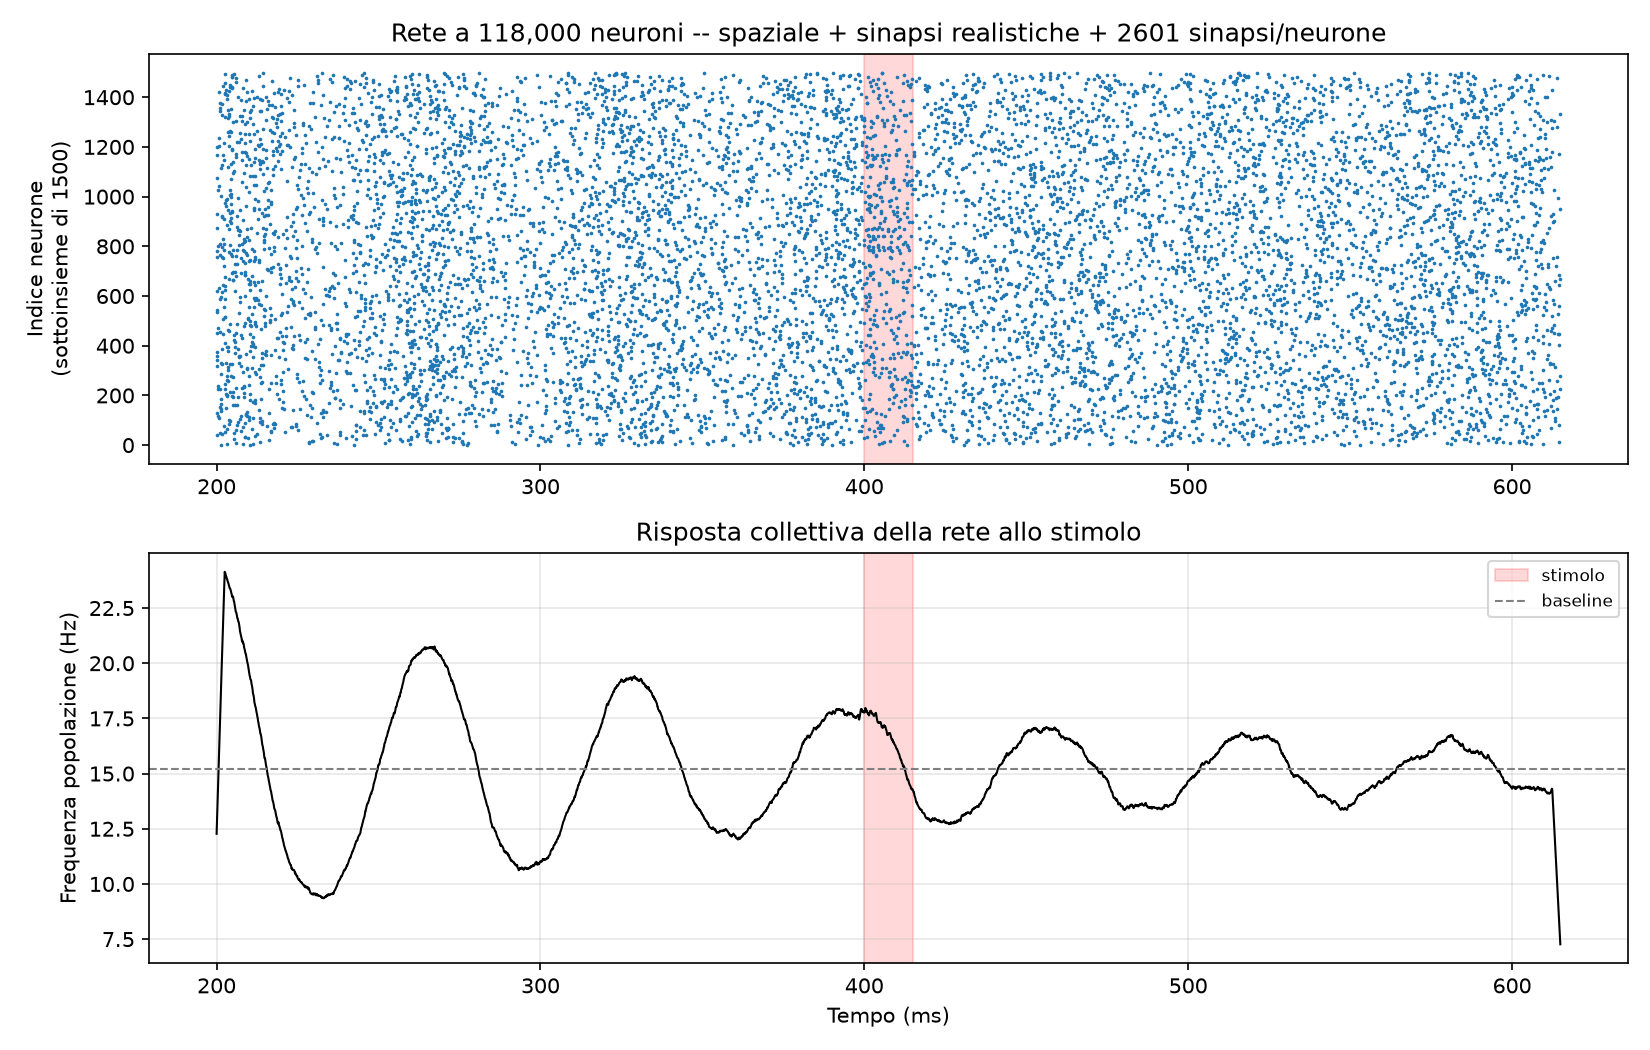
\includegraphics[width=6in,height=3.81818in]{media/media/image19.png}

\emph{Fig. 19 --- Final network (118,000 neurons, spatial + conductance + Allen density): raster and collective response, after the weight correction.}

The plot reveals a qualitative detail not captured by the numerical metrics alone: the network shows a REGULAR, PERSISTENT oscillation for the entire duration of the simulation (period of roughly 65-70 milliseconds, approximately constant amplitude), different both from the first attempt\textquotesingle s unstable behavior (unboundedly growing amplitude) and from the irregular asynchronous behavior observed in simpler networks (Sections 2.8, 3.6). The stimulus (red band, 400-415ms) falls during a rising phase of the network\textquotesingle s natural cycle, making it visually hard to distinguish from the adjacent spontaneous peaks -\/- a phenomenon that would require statistical verification over multiple trials (analogous to Section 2.11\textquotesingle s PSTH) to characterize with confidence.

\subsection{6.6 3D visualization of the final network}\label{d-visualization-of-the-final-network}

The final network (118,000 neurons) was visualized interactively by exporting the spatial positions and activity over time of a subset of 7,867 neurons (one neuron in every 15, to keep the animation smooth in the browser), using the same tools developed for previous visualizations (Section 4.2). The resulting HTML file is self-contained and interactive (not included as text in this document given its interactive nature, but attached separately).

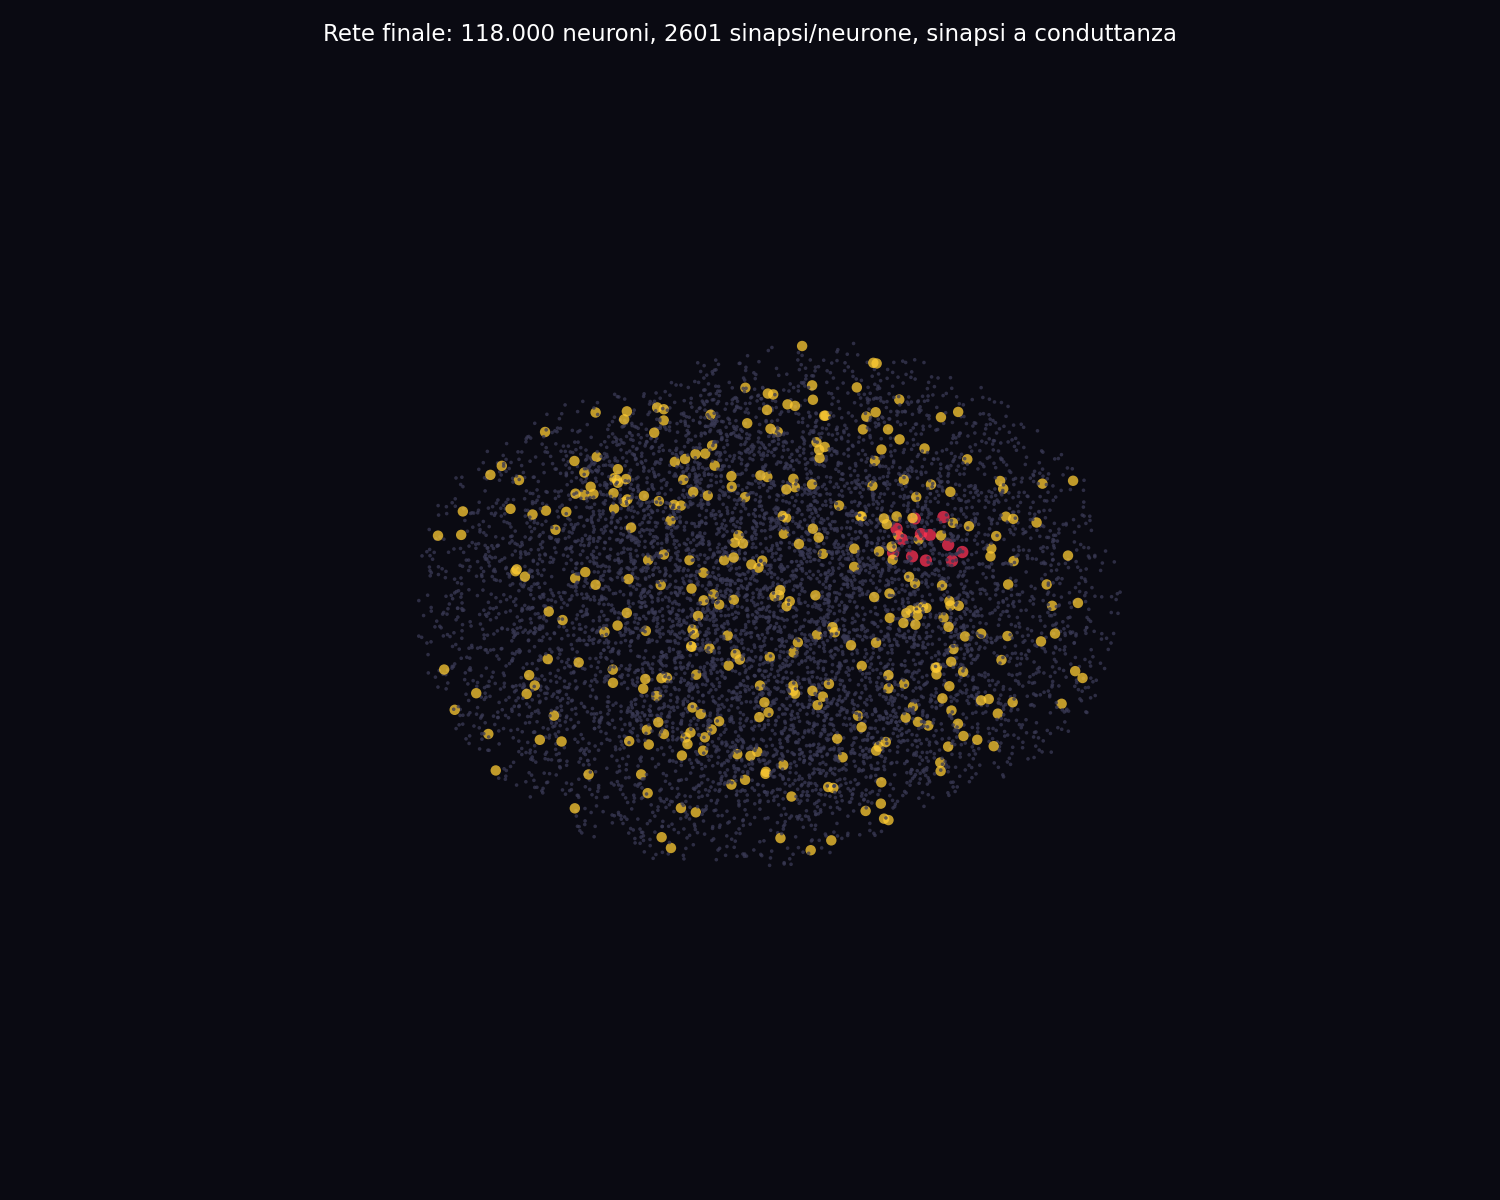
\includegraphics[width=4.3in,height=3.44in]{media/media/image20.png}

\emph{Fig. 20 --- Snapshot of the final network in 3D (7,867 neurons rendered out of 118,000).}

\textit{\textbf{Source code: rete\_\allowbreak{}sintesi\_\allowbreak{}export.py (version with 3D data export)}}

\lstinputlisting[language=Python]{scripts/rete_sintesi_export.py}
\subsection{6.7 Final comparison with the Allen Institute}\label{final-comparison-with-the-allen-institute}

{\def\LTcaptype{none} % do not increment counter
\begin{longtable}[]{@{}
  >{\raggedright\arraybackslash}p{(\linewidth - 6\tabcolsep) * \real{0.2500}}
  >{\raggedright\arraybackslash}p{(\linewidth - 6\tabcolsep) * \real{0.2500}}
  >{\raggedright\arraybackslash}p{(\linewidth - 6\tabcolsep) * \real{0.2500}}
  >{\raggedright\arraybackslash}p{(\linewidth - 6\tabcolsep) * \real{0.2500}}@{}}
\toprule\noalign{}
\begin{minipage}[b]{\linewidth}\raggedright
\end{minipage} & \begin{minipage}[b]{\linewidth}\raggedright
40M network (pure scale)
\end{minipage} & \begin{minipage}[b]{\linewidth}\raggedright
Final network (synthesis)
\end{minipage} & \begin{minipage}[b]{\linewidth}\raggedright
Allen Institute
\end{minipage} \\
\midrule\noalign{}
\endhead
\bottomrule\noalign{}
\endlastfoot
Neurons & 40,000,000 & 118,000 & \textasciitilde10,000,000 \\
Synapses/neuron & 31 & 2,601 & \textasciitilde2,600 \\
Synapse type & Voltage jump & Conductance & Conductance + morphology \\
Structure & Random & Spatial (3D small-world) & Real connectome \\
\% of mouse brain & 57.1\% & 0.169\% & \textasciitilde14.3\% \\
\end{longtable}
}

\textbf{The final comparison is honest on both fronts: on per-neuron synaptic density, this project reached PARITY with the Allen Institute (2,601 against \textasciitilde2,600); on the absolute number of neurons and on each one\textquotesingle s morphological detail, the gap remains wide. Neither of the two networks built in this project (the maximum-scale one and the maximum-density one) dominates the other on every axis at once -\/- a direct, concretely observed consequence of the shared-memory constraint discussed at the opening of this section (6.1).}

\section{7. Discussion}\label{discussion}

\subsection{7.1 Summary of the complete path}\label{summary-of-the-complete-path}

The path described in this document made it possible to build, experimentally verify, and personally observe a sequence of sixteen neural phenomena and experiments of steadily increasing complexity, always starting from minimal models and adding just one element of complexity at a time: basic synaptic communication, activation threshold, short-term plasticity, chain propagation, temporal summation, Hebbian learning via STDP, elementary pattern classification, balanced collective activity in a 300-neuron population, homeostasis after perturbation, modular organization, rigorous statistical verification, scaling up to 40 million neurons, structured spatial connectivity, interactive 3D visualization, one failed and one successful attempt at building a neural attractor, chains of linked attractors, competition between alternatives, reinforcement learning, and finally a context-conditioned decision policy.

This summary, in its first draft, covered only the first half of the document (Sections 1-5.4). The work then continued along a distinct but connected arc: learned bidirectional communication in the spiking domain, from total failure to a complete solution (transmission switch, homeostatic normalization, emergency suppression -\/- Sections 5.6-5.17), extended to multiple simultaneous messages and to a three-population relay network (Sections 5.18-5.20). Grafted onto that same architecture is a second thread, this time in physics (Sections 5.21-5.41): the impact of clinical CNAO ion beams (Geant4, QBBC) on the neural ring, linked to the spiking architecture through a functional-knockout experiment that reveals a dose-response gradient verified across four independent physical scenarios and generalized beyond the specific choice of knockout size; functional recovery after damage and a point of no return when the damage is complete; a clinical RBE model (Kase\textquotesingle s Microdosimetric Kinetic Model, the same one used at NIRS/HIMAC in Chiba) implemented and validated against published data before being used; a limitation discovered and corrected in the reproducibility of the per-neuron dose map; and finally a nanodosimetric link (Geant4-DNA) verified end-to-end, from the secondary electrons actually produced in the affected neurons all the way to ionization clusters, consistent with the published literature. The same methodological discipline described in Section 7.2 -\/- verify empirically instead of assuming, document failed attempts as much as successful ones -\/- runs through both threads without interruption.

\subsection{7.2 The two most important methodological lessons}\label{the-two-most-important-methodological-lessons}

Looking back over the entire document, two methodological lessons stand out with particular clarity, repeated in different forms at different points in the work:

\subsubsection{6.2.1 The difference between "looks true" and "verified true"}\label{the-difference-between-looks-true-and-verified-true}

At least three times over the course of the project, a result that looked convincing at first glance turned out, after rigorous statistical verification, not to be supported by the data: propagation between modules in Section 2.11 (an apparent effect of +13 Hz, which turned out to be only +0.89 Hz once averaged over 25 independent trials, well within the background noise of \textasciitilde4 Hz); the attempted STDP-based persistence in Section 4.3 (activity apparently present in a single, non-repeated trial, which turned out to be systematically zero over 16 correctly randomized independent trials); and the symmetry breaking in the equal-weights competition of Section 5.2.1 (apparently a "winning" candidate for some structural reason, which turned out to be a deterministic numerical artifact masked by insufficient noise). In all three cases, the gap between the initial impression and the verified result emerged only by applying the correct statistical tools (repetition, controlled randomization, comparison with the system\textquotesingle s natural variability) -\/- not through intuition or a closer visual inspection of a single plot.

\subsubsection{6.2.2 Failed attempts are part of the knowledge produced, not noise to hide}\label{failed-attempts-are-part-of-the-knowledge-produced-not-noise-to-hide}

The STDP-based attractor attempt (Section 4.3) and the first two architecture attempts for the ring attractor (Section 4.4.1, items 1 and 2) failed completely before the third attempt succeeded. Reporting these failures in detail -\/- including the mistaken hypotheses that motivated them and the precise technical reasons they did not work -\/- is not a flaw in the document, but an integral part of its value: it shows the real process by which scientific knowledge is built, one that rarely proceeds in a straight line from problem to solution.

\subsection{7.3 What is missing for real brain-like functionality}\label{what-is-missing-for-real-brain-like-functionality}

Even the project\textquotesingle s most advanced result (the contextual decision policy of Section 5.4) remains at an enormous distance from anything one could honestly call "brain-like functionality" in the full sense of the term. The missing ingredients, in roughly increasing order of difficulty to add:

\begin{itemize}
\item
  Real structured connectivity (a true connectome) instead of a simplified geometric model -\/- probably the single biggest challenge, still the subject of active research worldwide with the best tools available (see Section 4.5)
\item
  Diversity of cell types -\/- a real brain has hundreds of morphologically and functionally distinct neuron types, not just the two homogeneous categories (excitatory/inhibitory) used in this project
\item
  Structured, meaningful sensory input and motor output from the real world, instead of the Poisson-type random noise used as "background activity" in every experiment in this project
\item
  Neuromodulation (dopamine, serotonin, acetylcholine, noradrenaline), which operates on timescales much slower than individual electrical impulses, dynamically regulating the plasticity and excitability of entire neuronal populations as a function of behavioral state
\item
  Development and learning over timescales of months or years, not the few seconds of simulated time used in every experiment in this project
\item
  Generalization to never-before-seen situations -\/- the weights{[}context{]}{[}candidate{]} table of Section 5.4 is an associative memory (a lookup table), not an abstract representation that would allow correct interpolation or generalization to an intermediate context never presented during training
\end{itemize}

\section{8. Limitations of the work}\label{limitations-of-the-work}

\begin{itemize}
\item
  The Izhikevich model is a deliberate simplification: it does not include the neuron\textquotesingle s real morphology (dendritic structure, axonal geometry), nor the diversity of ion channels present in real biological neurons -\/- chosen out of the need to scale to millions of neurons, at the cost of lower biophysical realism than models such as Hodgkin-Huxley
\item
  Synaptic connections in most experiments have a static, "instantaneous" weight (apart from the explicit plasticity experiments, Sections 2.3, 2.6, 2.7), without realistic neurotransmitter-release dynamics such as short-term depression or postsynaptic receptor saturation
\item
  The inter-module propagation effect (Sections 2.10-2.11) deserves to be retested with stronger inter-module connectivity parameters, to find out whether a real effect emerges more clearly with denser connections, or whether the weakness observed at 2\% connectivity is a robust result that holds even at higher connectivity
\item
  The 40-million-neuron network (Section 3) uses the same fixed-degree random connectivity as the much smaller networks -\/- a genuine structural approach toward a mouse brain would require combining the scale reached with the spatial connectivity developed separately in Section 4, something the project did not have time to achieve jointly at full scale
\item
  Thermal-throttling slowdown (Section 3.4) introduces a not-fully-controlled hardware variable in the longer experiments, making time estimates for future experiments of comparable scale inherently uncertain
\item
  The systematic position bias (\textasciitilde0.045 units) repeatedly observed in the ring-attractor experiments (Sections 4.4.2, 5.1, 5.2) has not been fully diagnosed at its root -\/- probably a discretization artifact of the N=200-point grid, but without a formal check ruling it out as a real effect of the model
\item
  The contextual policy of Section 5.4 was verified on only 3 discrete, well-separated contexts on the ring -\/- it was not tested whether the mechanism generalizes to a larger number of contexts, to contexts spatially closer together (which could interfere with each other), or to the ability to correctly interpolate for an intermediate context never presented during training
\item
  None of this project\textquotesingle s experiments includes a cross-validation phase or a test set completely separate from training -\/- a standard machine-learning practice for ruling out overfitting, not systematically applied here given the exploratory nature of the work
\end{itemize}

The limitations above concern the pure-neuroscience thread (Sections 1-5.20). The connected physics thread (Geant4/CNAO/Chiba, Sections 5.21-5.41) has its own, distinct ones: the per-neuron dose map is fundamentally limited by counting statistics (each neuron, 10um radius, intercepts on average only 1-2 direct primaries out of 500,000 simulated events -\/- a limitation quantified in Section 5.37, not solvable with a 10x increase in statistics; a factor of 100-1000 would likely be needed, computationally prohibitive with QBBC\textquotesingle s full hadronic physics within this project\textquotesingle s time constraints).

The RBE model (Section 5.34) is the real Kase Microdosimetric Kinetic Model, no longer an ad hoc approximation, but remains simplified relative to the full clinical model in two stated respects: it uses the dose-averaged LET as a proxy for the dose-mean lineal energy (which would require a spectrum measured with a TEPC or a true site-level microdosimetric simulation), and it computes the saturation correction in the single-value-spectrum limit instead of integrating a full spectrum.

The functional knockout (Sections 5.22-5.38) remains a deliberately simplified model of neuronal damage -\/- complete removal of outgoing synapses above a relative dose threshold, not a validated biological-damage model (no absolute dose threshold for inactivating a single neuron is established in the literature, the same limitation stated in the Villagrasa/Baiocco paper that the twin project geant4dna\_\allowbreak{}icsd reproduces).

The nanodosimetric link (Sections 5.39-5.41) stops at the level of ICSD (Ionization Cluster Size Distribution) -\/- it does not model DNA damage (single or double breaks, SSB/DSB), which would require a geometric cell-nucleus model with multi-scale chromatin (available in Geant4-DNA, e.g. the official dnadamage1/molecularDNA examples, but not integrated here).

\section{9. Possible future developments}\label{possible-future-developments}

\begin{itemize}
\item
  Combine the scale already reached (Section 3, 40 million neurons) with the spatial connectivity developed separately (Section 4), to obtain a network that is simultaneously large AND structured -\/- the natural next step toward getting closer to a real mouse brain on both axes of realism
\item
  Make the connections between the two ring attractors of Section 5.1 plastic (STDP) as well, to study whether and how the associative map\textquotesingle s offset could itself be LEARNED by the system instead of being fixed externally beforehand
\item
  Repeat the rigorous statistical verification (PSTH technique, Section 2.11) on the attractor and reinforcement-learning experiments of Sections 4 and 5 as well, to check the statistical robustness of the positive results obtained over a relatively limited number of trials (6-18 depending on the experiment)
\item
  Extend the contextual policy (Section 5.4) to a larger number of contexts, and explicitly test the ability to generalize to intermediate contexts never seen during training -\/- the true test for distinguishing a pure associative memory from the beginnings of an abstract representation
\item
  Explore a network topology with more than two modules (Section 2.10), with connectivity patterns inspired by real published cortical connectivity maps (for example those of the Allen Institute, Section 4.5.2), instead of the artificial geometric kernel used in this project
\item
  Test access to a university computing cluster (for example through CNAO or the University of Pavia\textquotesingle s Physics Department) to overcome the RAM limit of a personal laptop, empirically verified in Section 3.3 at around 40-50 million neurons with simple random connectivity
\item
  Formally investigate the origin of the systematic position bias observed in the ring attractor (Sections 4.4.2, 5.1, 5.2), to determine whether it is a purely numerical artifact or reflects a real (if unwanted) property of the discretized model
\end{itemize}

The future developments above concern the pure-neuroscience thread. For the physics thread (Geant4/CNAO/Chiba), the open items remain those of the twin project geant4dna\_\allowbreak{}icsd (see its README): implementing the "common" cross-section dataset defined in the Villagrasa/Baiocco paper (requires extracting the numerical values from the supplementary material and writing a dedicated G4VEmModel subclass -\/- substantial work, not a weekend extension, as the paper itself notes) and, above all, extending the already-verified physical chain (macroscopic dose -\textgreater{} secondary-electron spectrum -\textgreater{} nanodosimetric ICSD) all the way to DNA damage (SSB/DSB) with a geometric cell-nucleus model -\/- the natural next step to make the link clinically interpretable, not just physically coherent. {[}Update: SSB/DSB damage was completed in Section 5.42, using the moleculardna example instead of dnadamage1/molecularDNA (blocked by a missing external dependency) -\/- only the paper\textquotesingle s common cross-section dataset remains open.{]}

\section{10. Glossary of technical terms used in the document}\label{glossary-of-technical-terms-used-in-the-document}

Attractor: A state (or set of states) toward which a dynamical system converges over time, and to which it returns after small perturbations. The ring attractor of Section 4.4 is the concrete example built in this project.

Multi-armed bandit: A classic reinforcement-learning problem in which an agent must repeatedly choose among several alternatives ("arms"), each with a different, unknown average reward, learning which to choose more often through repeated trials.

Excitation-inhibition balance (E/I balance): The ratio and dynamic equilibrium between excitatory neurons (which push other neurons toward spiking) and inhibitory ones (which suppress them) in a network, necessary to obtain stable activity instead of explosion or silence.

Brian2: A Python library for simulating spiking neural networks, used for every spiking experiment in this project.

Bump attractor: A specific type of neural attractor in which the stable state is a localized region of elevated activity ("the bump") on a broader spatial substrate, typically a ring or a grid. See Section 4.4.

Connectome: The complete map of synaptic connections among all the neurons of a nervous system (or a portion of it).

Standard deviation: A statistical measure of the spread of a set of values around their mean -\/- used repeatedly in this document to distinguish a real effect from random noise.

Izhikevich model: A two-coupled-differential-equation mathematical neuron model, proposed by Eugene Izhikevich in 2003. See Section 1.2.

KD-tree: A data structure that organizes points in a K-dimensional space to allow efficient spatial nearest-neighbor searches, used in Section 4.2 to compute the spatial connectivity of networks with up to 1 million neurons.

Homeostasis: A system\textquotesingle s ability to return to a stable equilibrium state after a perturbation, without external intervention. First observed in Section 2.9.

PSTH (Peristimulus Time Histogram): A standard statistical technique in experimental neuroscience for measuring a system\textquotesingle s average response to a stimulus, by averaging over many independent repetitions aligned to the moment of the stimulus. See Section 2.11.

Rescorla-Wagner rule: A historic (1972) mathematical model of associative learning, in which the strength of an association is updated in proportion to the difference between the reward received and the reward expected. Used as the basis for the update rule in Section 5.3.

Ring attractor: A neural attractor implemented on a ring topology, where the bump\textquotesingle s position encodes a continuous variable (for example a spatial position or an orientation). See Section 4.4.

Small-world (topology): A network organization pattern characterized by dense local connections combined with rare long-distance connections, observed in a great many real biological and social systems. Proposed by Watts and Strogatz in 1998. See Section 4.1.

Spike / action potential: The electrical impulse a neuron generates when its membrane potential crosses a threshold, the fundamental mechanism of communication between neurons.

STDP (Spike-Timing-Dependent Plasticity): A synaptic learning rule in which the strengthening or weakening of a synapse depends on the precise temporal order between presynaptic and postsynaptic spikes. See Section 2.6.

Winner-take-all: A computational mechanism, typically implemented via global or lateral inhibition, in which only one element (or a small subset) of a competitive system can remain active, suppressing all other candidates.

\section{11. Materials and reproducibility}\label{materials-and-reproducibility}

Every Python script developed during the project was verified by actually running it (not just writing it) and is fully reproducible. The complete or near-complete source code of each main script is included in the body of this document, in its corresponding section; the list below summarizes them with a reference to the section where they are discussed.

{\def\LTcaptype{none} % do not increment counter
\begin{longtable}[]{@{}
  >{\raggedright\arraybackslash}p{(\linewidth - 4\tabcolsep) * \real{0.3333}}
  >{\raggedright\arraybackslash}p{(\linewidth - 4\tabcolsep) * \real{0.3333}}
  >{\raggedright\arraybackslash}p{(\linewidth - 4\tabcolsep) * \real{0.3333}}@{}}
\toprule\noalign{}
\begin{minipage}[b]{\linewidth}\raggedright
File
\end{minipage} & \begin{minipage}[b]{\linewidth}\raggedright
Section
\end{minipage} & \begin{minipage}[b]{\linewidth}\raggedright
Content
\end{minipage} \\
\midrule\noalign{}
\endhead
\bottomrule\noalign{}
\endlastfoot
due\_\allowbreak{}neuroni.py & 2.1 & Basic communication between two neurons \\
esplorazione\_\allowbreak{}parametri.py & 2.2 & Synaptic threshold \\
plasticita\_\allowbreak{}sinaptica.py & 2.3 & Short-term facilitation \\
rete\_\allowbreak{}catena.py & 2.4 & Chain propagation \\
rete\_\allowbreak{}convergente.py & 2.5 & Temporal summation \\
stdp.py & 2.6 & Spike-Timing-Dependent Plasticity \\
classificazione\_\allowbreak{}stdp.py & 2.7 & Selective pattern learning \\
rete\_\allowbreak{}300\_\allowbreak{}neuroni.py & 2.8 & Balanced E/I network \\
rete\_\allowbreak{}300\_\allowbreak{}stimolo.py & 2.9 & Response to stimulus and recovery \\
due\_\allowbreak{}moduli.py & 2.10 & Modular architecture \\
psth\_\allowbreak{}moduli.py & 2.11 & Statistical verification over 25 trials \\
scaling\_\allowbreak{}verso\_\allowbreak{}topo.py, scaling\_\allowbreak{}fase2/3/4.py & 3.5 & Automatic progressive scaling \\
rete\_\allowbreak{}40M\_\allowbreak{}finale.py & 3.6 & Final experiment at 40 million neurons \\
rete\_\allowbreak{}smallworld.py & 4.1 & Small-world connectivity on a ring \\
brain3d\_\allowbreak{}visualization.html, brain1M\_\allowbreak{}visualization.html & 4.2 & Interactive 3D visualizations \\
ring\_\allowbreak{}attractor\_\allowbreak{}rate.py & 4.4 & Ring attractor, final verified result \\
chained\_\allowbreak{}attractors.py & 5.1 & Chain of two linked attractors \\
competing\_\allowbreak{}targets.py & 5.2 & Competition between alternatives \\
rl\_\allowbreak{}bandit.py & 5.3 & Reinforcement learning (bandit) \\
contextual\_\allowbreak{}policy.py & 5.4 & Contextual decision policy \\
rete\_\allowbreak{}sintesi\_\allowbreak{}export.py & 6.4-6.6 & Final synthesis: spatial + conductance + Allen density \\
dialogo\_\allowbreak{}ring\_\allowbreak{}attractor.py & 5.5.1 & Turn-based exchange between two rings, fixed channels \\
dialogo\_\allowbreak{}stdp.py & 5.5.2 & Learned A-\textgreater B synapse (turn-grained Hebbian); B-\textgreater A asymmetry documented \\
dialogo\_\allowbreak{}stdp\_\allowbreak{}adattamento.py & 5.5.3 & Adaptation + warm-up: both channels 100\% reliable \\
dialogo\_\allowbreak{}multi\_\allowbreak{}messaggio.py & 5.5.4 & Multiple messages on the same synapse: interference test \\
dialogo\_\allowbreak{}multi\_\allowbreak{}normalizzato.py & 5.5.5 & Homeostatic normalization on W\_\allowbreak{}AB: competition made visible, not resolved \\
dialogo\_\allowbreak{}multi\_\allowbreak{}repulsione.py & 5.5.6 & Repulsive exploration: interference resolved, 7 of 8 exchanges at 100\% \\
diagnosi\_\allowbreak{}bias\_\allowbreak{}posizione.py & 5.5.7 & Direct test (and refutation) of the position-bias hypothesis \\
dialogo\_\allowbreak{}multi\_\allowbreak{}repulsione\_\allowbreak{}3msg.py & 5.5.8 & Scaling to 3 messages: better separation, worse consolidation (open result) \\
dialogo\_\allowbreak{}multi\_\allowbreak{}scoperta\_\allowbreak{}locale.py & 5.5.9 & Repulsion only for discovery + local exploration: 10/12 exchanges, best result \\
dialogo\_\allowbreak{}multi\_\allowbreak{}scoperta\_\allowbreak{}locale\_\allowbreak{}montecarlo.py & 5.5.10 & Monte Carlo verification (8 seeds): 91.7\% success, but the hypothesis about the residual was wrong \\
dialogo\_\allowbreak{}multi\_\allowbreak{}scoperta\_\allowbreak{}locale\_\allowbreak{}permutazione.py & 5.5.11 & Position/value disambiguation: turn 5 follows order, turn 7 follows value \\
dialogo\_\allowbreak{}multi\_\allowbreak{}scoperta\_\allowbreak{}locale\_\allowbreak{}mischiato.py & 5.5.12 & Shuffled round-robin order: fairer across messages, but lower aggregate rate (87.5\% vs 91.7\%) \\
dialogo\_\allowbreak{}multi\_\allowbreak{}scoperta\_\allowbreak{}bidirezionale.py & 5.5.13 & Discovery+local consolidation on both channels: 95.8\%, turn 7 resolved at 100\% \\
ring\_\allowbreak{}attractor\_\allowbreak{}spiking.py & 5.6 & First stable spiking ring attractor (10 tuning attempts, NMDA-like synapses) \\
dialogo\_\allowbreak{}spiking.py & 5.7 & Learned A-\textgreater B communication between two spiking ring attractors, true STDP \\
dialogo\_\allowbreak{}spiking\_\allowbreak{}bidirezionale.py & 5.8 & Attempt at spiking bidirectionality: same asymmetry as the rate model, unresolved \\
dialogo\_\allowbreak{}spiking\_\allowbreak{}bidirezionale\_\allowbreak{}turni.py & 5.9 & A/B turn-taking scheme to isolate the confound in the spiking B-\textgreater A channel \\
dialogo\_\allowbreak{}spiking\_\allowbreak{}bidirezionale\_\allowbreak{}gate.py & 5.9 & B-\textgreater A plasticity confined to unconfounded turns: definitive negative conclusion \\
dialogo\_\allowbreak{}spiking\_\allowbreak{}multi.py & 5.10 & Two messages in the spiking domain, true STDP: no interference \\
dialogo\_\allowbreak{}spiking\_\allowbreak{}multi\_\allowbreak{}montecarlo.py & 5.11 & Monte Carlo verification (8 seeds): no spiking interference confirmed 16/16 \\
diagnosi\_\allowbreak{}sottosoglia\_\allowbreak{}ba.py & 5.12 & Sub-threshold check of the B-\textgreater A channel: confounded by A\textquotesingle s own dynamics \\
diagnosi\_\allowbreak{}ablazione\_\allowbreak{}ba.py & 5.12 & Ablation: a strong B-\textgreater A channel causes a numerical explosion, not a causal signal \\
dialogo\_\allowbreak{}spiking\_\allowbreak{}bidirezionale\_\allowbreak{}silenzia.py & 5.12 & Active silencing of A: same explosion, final conclusion \\
dialogo\_\allowbreak{}spiking\_\allowbreak{}bidirezionale\_\allowbreak{}interruttore.py & 5.13 & Transmission switch: stable with low weights, one seed out of four \\
diagnosi\_\allowbreak{}unidirezionale\_\allowbreak{}pesi\_\allowbreak{}forti.py & 5.13 & Control: a unidirectional channel with strong weights is stable on its own \\
dialogo\_\allowbreak{}spiking\_\allowbreak{}bidirezionale\_\allowbreak{}interruttore\_\allowbreak{}mc.py & 5.13 & Monte Carlo verification (4 seeds): only 1/4 stable, the \textquotesingle win\textquotesingle{} was a lucky case \\
dialogo\_\allowbreak{}spiking\_\allowbreak{}bidirezionale\_\allowbreak{}omeostasi.py & 5.14 & Homeostatic weight normalization: stable spiking bidirectionality on the base seed \\
dialogo\_\allowbreak{}spiking\_\allowbreak{}bidirezionale\_\allowbreak{}omeostasi\_\allowbreak{}mc.py & 5.14 & Monte Carlo verification (8 seeds): 6/8 stable, real but incomplete improvement \\
dialogo\_\allowbreak{}spiking\_\allowbreak{}bidirezionale\_\allowbreak{}omeostasi\_\allowbreak{}v2.py & 5.15 & More reactive homeostasis: clean bidirectional growth on the base seed \\
dialogo\_\allowbreak{}spiking\_\allowbreak{}bidirezionale\_\allowbreak{}omeostasi\_\allowbreak{}v2\_\allowbreak{}mc.py & 5.15 & Monte Carlo verification (8 seeds): 7/8 stable, better than v1 \\
diagnosi\_\allowbreak{}seed301\_\allowbreak{}anello\_\allowbreak{}isolato.py & 5.16 & Verification: seed 301\textquotesingle s isolated ring is stable on its own \\
dialogo\_\allowbreak{}spiking\_\allowbreak{}bidirezionale\_\allowbreak{}omeostasi\_\allowbreak{}v3.py & 5.16 & Emergency switch layered on gradual homeostasis \\
dialogo\_\allowbreak{}spiking\_\allowbreak{}bidirezionale\_\allowbreak{}omeostasi\_\allowbreak{}v3\_\allowbreak{}mc.py & 5.16 & Monte Carlo verification (8 seeds): 7/8 clean, eighth improved 40x \\
dialogo\_\allowbreak{}spiking\_\allowbreak{}bidirezionale\_\allowbreak{}omeostasi\_\allowbreak{}v4.py & 5.17 & Spiking bidirectionality solved: transmission switch + homeostasis + direct suppression \\
dialogo\_\allowbreak{}spiking\_\allowbreak{}bidirezionale\_\allowbreak{}omeostasi\_\allowbreak{}v4\_\allowbreak{}mc.py & 5.17 & Monte Carlo verification (8 seeds): 8/8 stable, bidirectional growth in every run \\
dialogo\_\allowbreak{}spiking\_\allowbreak{}bidirezionale\_\allowbreak{}multi.py & 5.18 & Multiple bidirectional spiking messages: completing the thread \\
dialogo\_\allowbreak{}spiking\_\allowbreak{}bidirezionale\_\allowbreak{}multi\_\allowbreak{}mc.py & 5.18 & Monte Carlo verification (8 seeds): 8/8 stable, no interference \\
dialogo\_\allowbreak{}spiking\_\allowbreak{}bidirezionale\_\allowbreak{}multi3.py & 5.19 & Three bidirectional spiking messages: load stress-test \\
dialogo\_\allowbreak{}spiking\_\allowbreak{}bidirezionale\_\allowbreak{}multi3\_\allowbreak{}mc.py & 5.19 & Monte Carlo verification (8 seeds): 8/8 stable, 98\% localization under threshold \\
dialogo\_\allowbreak{}spiking\_\allowbreak{}relay\_\allowbreak{}3anelli.py & 5.20 & Three-population relay A-\textgreater B-\textgreater C-\textgreater A, first step beyond the pair \\
dialogo\_\allowbreak{}spiking\_\allowbreak{}relay\_\allowbreak{}3anelli\_\allowbreak{}mc.py & 5.20 & Monte Carlo verification (6 seeds): information preserved over two hops in every case \\
dialogo\_\allowbreak{}spiking\_\allowbreak{}cnao\_\allowbreak{}knockout.py & 5.22 & Knockout of the highest-CNAO-dose neurons: selectively disrupts the message that uses them \\
dialogo\_\allowbreak{}spiking\_\allowbreak{}cnao\_\allowbreak{}knockout\_\allowbreak{}mc.py & 5.23 & Monte Carlo verification (8 seeds): knockout robust, 8/8 same direction \\
dialogo\_\allowbreak{}spiking\_\allowbreak{}knockout\_\allowbreak{}controllo\_\allowbreak{}mc.py & 5.24 & Negative control: random knockout does not reproduce the selective effect \\
braggProfile/braggProfile.cc & 5.25 & Depth-dose profile: finds the Bragg peak, discovers a geometric artifact in cnaoRingImpact \\
dialogo\_\allowbreak{}spiking\_\allowbreak{}cnao\_\allowbreak{}knockout\_\allowbreak{}v2\_\allowbreak{}mc.py & 5.26 & Re-verification with corrected dose: the effect flips as predicted (falsifiable test passed) \\
dialogo\_\allowbreak{}spiking\_\allowbreak{}cnao\_\allowbreak{}knockout\_\allowbreak{}picco\_\allowbreak{}mc.py & 5.27 & Complete dataset at the peak + dose-response gradient across three overlap levels \\
dialogo\_\allowbreak{}spiking\_\allowbreak{}cnao\_\allowbreak{}knockout\_\allowbreak{}proton\_\allowbreak{}mc.py & 5.28 & Knockout with a proton dose map: strongest effect so far (7.07x, 8/8), complete 4-point gradient \\
dialogo\_\allowbreak{}spiking\_\allowbreak{}cnao\_\allowbreak{}recupero.py & 5.29 & Functional recovery after knockout: residual plasticity progressively compensates, verified over 4 seeds \\
dialogo\_\allowbreak{}spiking\_\allowbreak{}lesione\_\allowbreak{}completa\_\allowbreak{}mc.py & 5.30 & Complete lesion of the encoding zone: the recovery seen in 5.29 disappears, point of no return confirmed over 5 runs (1+4 MC) \\
geant4\_\allowbreak{}cnao\_\allowbreak{}ring (RunAction.cc + RBE analysis) & 5.31 & RBE-LET model (Kanai/NIRS): the 5.22-5.28 gradient holds within the same depth; discovered Monte Carlo variability between physical runs not yet verified \\
geant4\_\allowbreak{}cnao\_\allowbreak{}ring (cnaoRingImpact.cc, explicit seed) & 5.32 & Discovered: the per-neuron dose map is dominated by Monte Carlo noise (overlap 1.0/10 over 4 seeds); the neuroscience causal mechanism remains valid, the single-neuron-level correspondence does not \\
dialogo\_\allowbreak{}spiking\_\allowbreak{}cnao\_\allowbreak{}knockout\_\allowbreak{}media4seed\_\allowbreak{}mc.py & 5.33 & Knockout from dose averaged over 4 Geant4 seeds: 1-vs-0 overlap indistinguishable from the negative control, a minimum imbalance threshold (\textasciitilde2 neurons) emerges for a real effect \\
geant4\_\allowbreak{}cnao\_\allowbreak{}ring/analysis/mkm\_\allowbreak{}rbe.py & 5.34 & Real Kase/NIRS MKM model (no longer 5.31\textquotesingle s linear approximation), validated against published data within 10-15\%; confirms 5.31 with a true clinical model \\
geant4\_\allowbreak{}cnao\_\allowbreak{}ring/analysis/mkm\_\allowbreak{}rbe.py (full dataset) & 5.35 & MKM across all six CNAO configurations: physical/biological overlap 9-10/10 everywhere; carbon overkill and anomalous 150 MeV proton RBE \\
geant4\_\allowbreak{}cnao\_\allowbreak{}ring/src/SteppingAction.cc (CNAO\_\allowbreak{}DEBUG\_\allowbreak{}NEURON diagnostic) & 5.36 & Empirically verified (not just hypothesized) the 5.35 anomalous LET peak: it is the primary proton nearly stopped (range straggling), not a secondary fragment -\/- linked to the real debate over variable RBE at the distal edge in proton therapy \\
build/results\_\allowbreak{}highstat/ (carbon 5M events, seed 501/502) & 5.37 & Quantified: 10x events improves overlap from 1.0/10 (pure noise) to 2/10 -\/- not enough; confirms that averaging over seeds (5.33) is more efficient than increasing events \\
dialogo\_\allowbreak{}spiking\_\allowbreak{}cnao\_\allowbreak{}knockout\_\allowbreak{}top5\_\allowbreak{}mc.py / top20\_\allowbreak{}mc.py & 5.38 & Knockout size (5, 10, 20 neurons) is not special: TOP-5 (0-vs-0 overlap) null as predicted, TOP-20 (reversed overlap) reverses the effect (1.74x, 7/8) exactly as predicted \\
geant4\_\allowbreak{}cnao\_\allowbreak{}ring (DetectorConstruction.cc, production cut) & 5.39 & First step of the nanodosimetric link: a bug (too-coarse production cut) discovered and fixed, real secondary-electron spectrum verified (100\% below 1 MeV, median 1.86 keV) -\/- the physical premise of coupling with Geant4-DNA is confirmed \\
geant4dna\_\allowbreak{}icsd/build/nanoICSD (real energies from 5.39) & 5.40 & Nanodosimetric link completed: ICSD from REAL (CNAO) secondary-electron energies fit coherently between the points already published in the Villagrasa/Baiocco paper -\/- macro-to-nano chain verified end-to-end \\
geant4dna\_\allowbreak{}icsd/nanoICSD.cc (explicit seed, 4-seed verification) & 5.41 & Monte Carlo verification of nanoICSD: M1=1.090 confirmed stable (CV 0.34\% over 4 seeds) -\/- unlike the dose map (5.32), no statistical-noise problem here \\
geant4dna\_\allowbreak{}ssbdsb (moleculardna, real energies from 5.39) & 5.42 & Real DNA damage (SSB/DSB) from CNAO secondary electrons: higher DSB fraction at low energy (higher LET), verified over 3 seeds (SB CV 1.8\%, DSB CV 12.4\%) -\/- closes the nanodosimetric link down to the DNA level \\
geant4dna\_\allowbreak{}ssbdsb/results/spectrum\_\allowbreak{}weighted (6 weighted points) & 5.43 & DNA damage weighted over the entire real spectrum (6 points, not 2): DSB fraction monotonic with energy (15.7\% to 5.4\%), final weighted average 9.5\% -\/- closes the last limitation stated in 5.42 \\
geant4\_\allowbreak{}cnao\_\allowbreak{}ring (per-neuron DSB tracking) & 5.44 & Physics-neuroscience bridge closed down to the DNA: per-neuron estimated-DSB-damage ranking overlaps 9/10 with the physical-dose ranking -\/- physical dose remains a robust criterion even at the deepest biological realism level reached \\
dialogo\_\allowbreak{}spiking\_\allowbreak{}relay\_\allowbreak{}chiusura\_\allowbreak{}turni\_\allowbreak{}mc.py & 5.45 & The C-\textgreater A loop does not close causally: verified over 5 runs (1+4 MC), never more than 3/10 probes with residual activity, always at noise level -\/- extends the 5.9 conclusion (B-\textgreater A not causal) to the three-ring case \\
\end{longtable}
}

\emph{Execution environment: Python 3.14, Brian2 2.10.1, NumPy, SciPy, Matplotlib, on a MacBook Air with an Apple M5 chip and 24 GB of RAM. The two interactive 3D visualizations require a modern web browser with WebGL support (recent versions of Chrome, Safari, Firefox) and are self-contained (the simulation data is embedded directly in the HTML file; no internet connection is required except for the initial loading of the Three.js library from a CDN).}

\emph{End of document.}

\end{document}
